\documentclass[twoside]{book}

% Packages required by doxygen
\usepackage{calc}
\usepackage{doxygen}
\usepackage{graphicx}
\usepackage[utf8]{inputenc}
\usepackage{makeidx}
\usepackage{multicol}
\usepackage{multirow}
\usepackage{fixltx2e}
\PassOptionsToPackage{warn}{textcomp}
\usepackage{textcomp}
\usepackage[nointegrals]{wasysym}
\usepackage[table]{xcolor}

% Font selection
\usepackage[T1]{fontenc}
\usepackage{mathptmx}
\usepackage[scaled=.90]{helvet}
\usepackage{courier}
\usepackage{amssymb}
\usepackage{sectsty}
\renewcommand{\familydefault}{\sfdefault}
\allsectionsfont{%
  \fontseries{bc}\selectfont%
  \color{darkgray}%
}
\renewcommand{\DoxyLabelFont}{%
  \fontseries{bc}\selectfont%
  \color{darkgray}%
}
\newcommand{\+}{\discretionary{\mbox{\scriptsize$\hookleftarrow$}}{}{}}

% Page & text layout
\usepackage{geometry}
\geometry{%
  a4paper,%
  top=2.5cm,%
  bottom=2.5cm,%
  left=2.5cm,%
  right=2.5cm%
}
\tolerance=750
\hfuzz=15pt
\hbadness=750
\setlength{\emergencystretch}{15pt}
\setlength{\parindent}{0cm}
\setlength{\parskip}{0.2cm}
\makeatletter
\renewcommand{\paragraph}{%
  \@startsection{paragraph}{4}{0ex}{-1.0ex}{1.0ex}{%
    \normalfont\normalsize\bfseries\SS@parafont%
  }%
}
\renewcommand{\subparagraph}{%
  \@startsection{subparagraph}{5}{0ex}{-1.0ex}{1.0ex}{%
    \normalfont\normalsize\bfseries\SS@subparafont%
  }%
}
\makeatother

% Headers & footers
\usepackage{fancyhdr}
\pagestyle{fancyplain}
\fancyhead[LE]{\fancyplain{}{\bfseries\thepage}}
\fancyhead[CE]{\fancyplain{}{}}
\fancyhead[RE]{\fancyplain{}{\bfseries\leftmark}}
\fancyhead[LO]{\fancyplain{}{\bfseries\rightmark}}
\fancyhead[CO]{\fancyplain{}{}}
\fancyhead[RO]{\fancyplain{}{\bfseries\thepage}}
\fancyfoot[LE]{\fancyplain{}{}}
\fancyfoot[CE]{\fancyplain{}{}}
\fancyfoot[RE]{\fancyplain{}{\bfseries\scriptsize Generated on Thu May 29 2014 21\+:57\+:24 for H\+A\+L by Doxygen }}
\fancyfoot[LO]{\fancyplain{}{\bfseries\scriptsize Generated on Thu May 29 2014 21\+:57\+:24 for H\+A\+L by Doxygen }}
\fancyfoot[CO]{\fancyplain{}{}}
\fancyfoot[RO]{\fancyplain{}{}}
\renewcommand{\footrulewidth}{0.4pt}
\renewcommand{\chaptermark}[1]{%
  \markboth{#1}{}%
}
\renewcommand{\sectionmark}[1]{%
  \markright{\thesection\ #1}%
}

% Indices & bibliography
\usepackage{natbib}
\usepackage[titles]{tocloft}
\setcounter{tocdepth}{3}
\setcounter{secnumdepth}{5}
\makeindex

% Hyperlinks (required, but should be loaded last)
\usepackage{ifpdf}
\ifpdf
  \usepackage[pdftex,pagebackref=true]{hyperref}
\else
  \usepackage[ps2pdf,pagebackref=true]{hyperref}
\fi
\hypersetup{%
  colorlinks=true,%
  linkcolor=blue,%
  citecolor=blue,%
  unicode%
}

% Custom commands
\newcommand{\clearemptydoublepage}{%
  \newpage{\pagestyle{empty}\cleardoublepage}%
}


%===== C O N T E N T S =====

\begin{document}

% Titlepage & ToC
\hypersetup{pageanchor=false,
             bookmarks=true,
             bookmarksnumbered=true,
             pdfencoding=unicode
            }
\pagenumbering{roman}
\begin{titlepage}
\vspace*{7cm}
\begin{center}%
{\Large H\+A\+L }\\
\vspace*{1cm}
{\large Generated by Doxygen 1.8.7}\\
\vspace*{0.5cm}
{\small Thu May 29 2014 21:57:24}\\
\end{center}
\end{titlepage}
\clearemptydoublepage
\tableofcontents
\clearemptydoublepage
\pagenumbering{arabic}
\hypersetup{pageanchor=true}

%--- Begin generated contents ---
\chapter{Welcome, to the H\+A\+L code reference.}
\label{index}\hypertarget{index}{}\hypertarget{index_intro_sec}{}\section{Introduction}\label{index_intro_sec}
This a custom R\-O\-O\-T library that provides a framework for physics analysis. It contains several functions and classes that aid in analyzing high energy physics data. To aid in the compilation of all the source code, a macro entitled {\ttfamily Compile\-Source.\-C} can be executed from the command line. All functions and classes are available in python from the {\ttfamily lib/\-H\-A\-L.\-py} module. Furthermore, everything lives in the 'H\-A\-L' namespace. H\-A\-L stands for\par
 H -\/ H.\-E.\-P.\par
 A -\/ Analysis\par
 L -\/ Library\par
 Of course, this is also a thinly veiled reference to the villian in the classic \char`\"{}2001\-: A Space Odyssey.\char`\"{} But, I personally think this bit of software is far less pernicious 
\chapter{Todo List}
\label{todo}
\hypertarget{todo}{}

\begin{DoxyRefList}
\item[\label{todo__todo000001}%
\hypertarget{todo__todo000001}{}%
Namespace \hyperlink{namespace_h_a_l}{H\+A\+L} ]Generic Algorithms\+: Add chi-\/squared minimization algorithm 

Generic Algorithms\+: Add parent selection algorithm 

Generic Algorithms\+: Add merging algorithm 

Generic Algorithms\+: Add monitor for User\+Data algorithm 

Generic Algorithms\+: Add parent/child traversal algorithms 

Generic Algorithms\+: Make error messages more informative 

Generic Algorithms\+: Add chi-\/squared minimization algorithm 

Generic Algorithms\+: Add parent selection algorithm 

Generic Algorithms\+: Add merging algorithm 

Generic Algorithms\+: Add monitor for User\+Data algorithm 

Generic Algorithms\+: Add parent/child traversal algorithms 

Generic Algorithms\+: Make error messages more informative 

Generic Algorithms\+: Add chi-\/squared minimization algorithm 

Generic Algorithms\+: Add parent selection algorithm 

Generic Algorithms\+: Add merging algorithm 

Generic Algorithms\+: Add monitor for User\+Data algorithm 

Generic Algorithms\+: Add parent/child traversal algorithms 

Generic Algorithms\+: Make error messages more informative 

Generic Algorithms\+: Make error messages more informative 

Generic Algorithms\+: Add chi-\/squared minimization algorithm 

Generic Algorithms\+: Add parent selection algorithm 

Generic Algorithms\+: Add merging algorithm 

Generic Algorithms\+: Add monitor for User\+Data algorithm 

Generic Algorithms\+: Add parent/child traversal algorithms 

Generic Algorithms\+: Make error messages more informative 

Generic Algorithms\+: Add chi-\/squared minimization algorithm 

Generic Algorithms\+: Add parent selection algorithm 

Generic Algorithms\+: Add merging algorithm 

Generic Algorithms\+: Add monitor for User\+Data algorithm 

Generic Algorithms\+: Add parent/child traversal algorithms 

Generic Algorithms\+: Make error messages more informative 

Generic Algorithms\+: Add chi-\/squared minimization algorithm 

Generic Algorithms\+: Add parent selection algorithm 

Generic Algorithms\+: Add merging algorithm 

Generic Algorithms\+: Add monitor for User\+Data algorithm 

Generic Algorithms\+: Add parent/child traversal algorithms 

Generic Algorithms\+: Make error messages more informative 

Generic Algorithms\+: Add chi-\/squared minimization algorithm 

Generic Algorithms\+: Add parent selection algorithm 

Generic Algorithms\+: Add merging algorithm 

Generic Algorithms\+: Add monitor for User\+Data algorithm 

Generic Algorithms\+: Add parent/child traversal algorithms 

Generic Algorithms\+: Make error messages more informative 

Generic Algorithms\+: Add chi-\/squared minimization algorithm 

Generic Algorithms\+: Add parent selection algorithm 

Generic Algorithms\+: Add merging algorithm 

Generic Algorithms\+: Add monitor for User\+Data algorithm 

Generic Algorithms\+: Add parent/child traversal algorithms 

Generic Algorithms\+: Make error messages more informative 

Generic Algorithms\+: Add chi-\/squared minimization algorithm 

Generic Algorithms\+: Add parent selection algorithm 

Generic Algorithms\+: Add merging algorithm 

Generic Algorithms\+: Add monitor for User\+Data algorithm 

Generic Algorithms\+: Add parent/child traversal algorithms 

Generic Algorithms\+: Make error messages more informative 

Generic Algorithms\+: Add chi-\/squared minimization algorithm 

Generic Algorithms\+: Add parent selection algorithm 

Generic Algorithms\+: Add merging algorithm 

Generic Algorithms\+: Add monitor for User\+Data algorithm 

Generic Algorithms\+: Add parent/child traversal algorithms 

Generic Algorithms\+: Make error messages more informative 

Generic Algorithms\+: Add chi-\/squared minimization algorithm 

Generic Algorithms\+: Add parent selection algorithm 

Generic Algorithms\+: Add merging algorithm 

Generic Algorithms\+: Add monitor for User\+Data algorithm 

Generic Algorithms\+: Add parent/child traversal algorithms 

Generic Algorithms\+: Make error messages more informative 
\end{DoxyRefList}
\chapter{Namespace Index}
\section{Namespace List}
Here is a list of all documented namespaces with brief descriptions\-:\begin{DoxyCompactList}
\item\contentsline{section}{\hyperlink{namespace_h_a_l}{H\-A\-L} }{\pageref{namespace_h_a_l}}{}
\end{DoxyCompactList}

\chapter{Hierarchical Index}
\section{Class Hierarchy}
This inheritance list is sorted roughly, but not completely, alphabetically\-:\begin{DoxyCompactList}
\item \contentsline{section}{H\-A\-L\-:\-:Algorithm}{\pageref{class_h_a_l_1_1_algorithm}}{}
\begin{DoxyCompactList}
\item \contentsline{section}{H\-A\-L\-:\-:Cut\-Algorithm}{\pageref{class_h_a_l_1_1_cut_algorithm}}{}
\item \contentsline{section}{H\-A\-L\-:\-:F\-A0000}{\pageref{class_h_a_l_1_1_f_a0000}}{}
\item \contentsline{section}{H\-A\-L\-:\-:Import\-T\-L\-V\-Algo}{\pageref{class_h_a_l_1_1_import_t_l_v_algo}}{}
\begin{DoxyCompactList}
\item \contentsline{section}{H\-A\-L\-:\-:I\-A0000}{\pageref{class_h_a_l_1_1_i_a0000}}{}
\item \contentsline{section}{H\-A\-L\-:\-:I\-A0001}{\pageref{class_h_a_l_1_1_i_a0001}}{}
\item \contentsline{section}{H\-A\-L\-:\-:I\-A0002}{\pageref{class_h_a_l_1_1_i_a0002}}{}
\item \contentsline{section}{H\-A\-L\-:\-:I\-A0010}{\pageref{class_h_a_l_1_1_i_a0010}}{}
\item \contentsline{section}{H\-A\-L\-:\-:I\-A0011}{\pageref{class_h_a_l_1_1_i_a0011}}{}
\item \contentsline{section}{H\-A\-L\-:\-:I\-A0012}{\pageref{class_h_a_l_1_1_i_a0012}}{}
\item \contentsline{section}{H\-A\-L\-:\-:I\-A0020}{\pageref{class_h_a_l_1_1_i_a0020}}{}
\item \contentsline{section}{H\-A\-L\-:\-:I\-A0021}{\pageref{class_h_a_l_1_1_i_a0021}}{}
\item \contentsline{section}{H\-A\-L\-:\-:I\-A0022}{\pageref{class_h_a_l_1_1_i_a0022}}{}
\end{DoxyCompactList}
\item \contentsline{section}{H\-A\-L\-:\-:Reconstruction\-Algorithm}{\pageref{class_h_a_l_1_1_reconstruction_algorithm}}{}
\begin{DoxyCompactList}
\item \contentsline{section}{H\-A\-L\-:\-:Python\-Reconstruction\-Algorithm}{\pageref{class_h_a_l_1_1_python_reconstruction_algorithm}}{}
\end{DoxyCompactList}
\end{DoxyCompactList}
\item \contentsline{section}{H\-A\-L\-:\-:Analysis}{\pageref{class_h_a_l_1_1_analysis}}{}
\item \contentsline{section}{H\-A\-L\-:\-:Cut\-Optimizer}{\pageref{class_h_a_l_1_1_cut_optimizer}}{}
\item exception\begin{DoxyCompactList}
\item \contentsline{section}{H\-A\-L\-:\-:H\-A\-L\-Exception}{\pageref{class_h_a_l_1_1_h_a_l_exception}}{}
\end{DoxyCompactList}
\item \contentsline{section}{H\-A\-L\-:\-:Integrator}{\pageref{class_h_a_l_1_1_integrator}}{}
\item \contentsline{section}{H\-A\-L\-:\-:Interp\-Base}{\pageref{class_h_a_l_1_1_interp_base}}{}
\begin{DoxyCompactList}
\item \contentsline{section}{H\-A\-L\-:\-:Poly\-Interp}{\pageref{class_h_a_l_1_1_poly_interp}}{}
\end{DoxyCompactList}
\item \contentsline{section}{H\-A\-L\-:\-:Poly2\-D\-Interp}{\pageref{class_h_a_l_1_1_poly2_d_interp}}{}
\item T\-Named\begin{DoxyCompactList}
\item \contentsline{section}{H\-A\-L\-:\-:Analysis\-Data}{\pageref{class_h_a_l_1_1_analysis_data}}{}
\begin{DoxyCompactList}
\item \contentsline{section}{H\-A\-L\-:\-:Analysis\-Tree\-Writer}{\pageref{class_h_a_l_1_1_analysis_tree_writer}}{}
\end{DoxyCompactList}
\item \contentsline{section}{H\-A\-L\-:\-:Analysis\-Tree\-Reader}{\pageref{class_h_a_l_1_1_analysis_tree_reader}}{}
\end{DoxyCompactList}
\item T\-Selector\begin{DoxyCompactList}
\item \contentsline{section}{H\-A\-L\-:\-:Analysis\-Selector}{\pageref{class_h_a_l_1_1_analysis_selector}}{}
\end{DoxyCompactList}
\end{DoxyCompactList}

\chapter{Class Index}
\section{Class List}
Here are the classes, structs, unions and interfaces with brief descriptions\+:\begin{DoxyCompactList}
\item\contentsline{section}{\hyperlink{class_h_a_l_1_1_algorithm}{H\+A\+L\+::\+Algorithm} }{\pageref{class_h_a_l_1_1_algorithm}}{}
\item\contentsline{section}{\hyperlink{class_h_a_l_1_1_analysis}{H\+A\+L\+::\+Analysis} }{\pageref{class_h_a_l_1_1_analysis}}{}
\item\contentsline{section}{\hyperlink{class_h_a_l_1_1_analysis_data}{H\+A\+L\+::\+Analysis\+Data} }{\pageref{class_h_a_l_1_1_analysis_data}}{}
\item\contentsline{section}{\hyperlink{class_h_a_l_1_1_analysis_selector}{H\+A\+L\+::\+Analysis\+Selector} }{\pageref{class_h_a_l_1_1_analysis_selector}}{}
\item\contentsline{section}{\hyperlink{class_h_a_l_1_1_analysis_tree_reader}{H\+A\+L\+::\+Analysis\+Tree\+Reader} }{\pageref{class_h_a_l_1_1_analysis_tree_reader}}{}
\item\contentsline{section}{\hyperlink{class_h_a_l_1_1_analysis_tree_writer}{H\+A\+L\+::\+Analysis\+Tree\+Writer} }{\pageref{class_h_a_l_1_1_analysis_tree_writer}}{}
\item\contentsline{section}{\hyperlink{class_h_a_l_1_1_algorithms_1_1_attach_attribute}{H\+A\+L\+::\+Algorithms\+::\+Attach\+Attribute} \\*\hyperlink{class_h_a_l_1_1_algorithm}{Algorithm} that attaches a decimal value to an existing set of particles }{\pageref{class_h_a_l_1_1_algorithms_1_1_attach_attribute}}{}
\item\contentsline{section}{\hyperlink{class_h_a_l_1_1_algorithms_1_1_cut}{H\+A\+L\+::\+Algorithms\+::\+Cut} \\*Generic algorithm class that cuts on particle multiplicity, bool, integer, counting, and decimal values }{\pageref{class_h_a_l_1_1_algorithms_1_1_cut}}{}
\item\contentsline{section}{\hyperlink{class_h_a_l_1_1_cut_algorithm}{H\+A\+L\+::\+Cut\+Algorithm} }{\pageref{class_h_a_l_1_1_cut_algorithm}}{}
\item\contentsline{section}{\hyperlink{class_h_a_l_1_1_cut_optimizer}{H\+A\+L\+::\+Cut\+Optimizer} }{\pageref{class_h_a_l_1_1_cut_optimizer}}{}
\item\contentsline{section}{\hyperlink{class_h_a_l_1_1_algorithms_1_1_empty_cut}{H\+A\+L\+::\+Algorithms\+::\+Empty\+Cut} \\*Generic algorithm class that serves as a baseline algorithm for any subsequent \hyperlink{class_h_a_l_1_1_algorithms_1_1_cut}{Cut} algorithms }{\pageref{class_h_a_l_1_1_algorithms_1_1_empty_cut}}{}
\item\contentsline{section}{\hyperlink{class_h_a_l_1_1_generic_data}{H\+A\+L\+::\+Generic\+Data} }{\pageref{class_h_a_l_1_1_generic_data}}{}
\item\contentsline{section}{\hyperlink{class_h_a_l_1_1_generic_particle}{H\+A\+L\+::\+Generic\+Particle} }{\pageref{class_h_a_l_1_1_generic_particle}}{}
\item\contentsline{section}{\hyperlink{class_h_a_l_1_1_h_a_l_exception}{H\+A\+L\+::\+H\+A\+L\+Exception} }{\pageref{class_h_a_l_1_1_h_a_l_exception}}{}
\item\contentsline{section}{\hyperlink{class_h_a_l_1_1_algorithms_1_1_import_bool_value}{H\+A\+L\+::\+Algorithms\+::\+Import\+Bool\+Value$<$ Value\+Getter $>$} \\*\hyperlink{class_h_a_l_1_1_algorithm}{Algorithm} that stores a boolean value from information in a T\+Tree }{\pageref{class_h_a_l_1_1_algorithms_1_1_import_bool_value}}{}
\item\contentsline{section}{\hyperlink{class_h_a_l_1_1_algorithms_1_1_import_counting_value}{H\+A\+L\+::\+Algorithms\+::\+Import\+Counting\+Value$<$ Value\+Getter $>$} \\*\hyperlink{class_h_a_l_1_1_algorithm}{Algorithm} that stores a counting value from information in a T\+Tree }{\pageref{class_h_a_l_1_1_algorithms_1_1_import_counting_value}}{}
\item\contentsline{section}{\hyperlink{class_h_a_l_1_1_algorithms_1_1_import_decimal_value}{H\+A\+L\+::\+Algorithms\+::\+Import\+Decimal\+Value$<$ Value\+Getter $>$} \\*\hyperlink{class_h_a_l_1_1_algorithm}{Algorithm} that stores a decimal value from information in a T\+Tree }{\pageref{class_h_a_l_1_1_algorithms_1_1_import_decimal_value}}{}
\item\contentsline{section}{\hyperlink{class_h_a_l_1_1_algorithms_1_1_import_integer_value}{H\+A\+L\+::\+Algorithms\+::\+Import\+Integer\+Value$<$ Value\+Getter $>$} \\*\hyperlink{class_h_a_l_1_1_algorithm}{Algorithm} that stores an integer value from information in a T\+Tree }{\pageref{class_h_a_l_1_1_algorithms_1_1_import_integer_value}}{}
\item\contentsline{section}{\hyperlink{class_h_a_l_1_1_algorithms_1_1_import_particle}{H\+A\+L\+::\+Algorithms\+::\+Import\+Particle} \\*\hyperlink{class_h_a_l_1_1_algorithm}{Algorithm} that builds particles from information in a T\+Tree }{\pageref{class_h_a_l_1_1_algorithms_1_1_import_particle}}{}
\item\contentsline{section}{\hyperlink{class_h_a_l_1_1_integrator}{H\+A\+L\+::\+Integrator} }{\pageref{class_h_a_l_1_1_integrator}}{}
\item\contentsline{section}{\hyperlink{class_h_a_l_1_1_interp_base}{H\+A\+L\+::\+Interp\+Base} }{\pageref{class_h_a_l_1_1_interp_base}}{}
\item\contentsline{section}{\hyperlink{class_h_a_l_1_1_algorithms_1_1_min_chi_squared_selection}{H\+A\+L\+::\+Algorithms\+::\+Min\+Chi\+Squared\+Selection} \\*\hyperlink{class_h_a_l_1_1_algorithm}{Algorithm} that performs a chi-\/squared minimization }{\pageref{class_h_a_l_1_1_algorithms_1_1_min_chi_squared_selection}}{}
\item\contentsline{section}{\hyperlink{class_h_a_l_1_1_algorithms_1_1_monitor_algorithm}{H\+A\+L\+::\+Algorithms\+::\+Monitor\+Algorithm} \\*Generic algorithm class that prints the content of an algorithm to a given ostream }{\pageref{class_h_a_l_1_1_algorithms_1_1_monitor_algorithm}}{}
\item\contentsline{section}{\hyperlink{class_h_a_l_1_1_algorithms_1_1_monitor_user_data}{H\+A\+L\+::\+Algorithms\+::\+Monitor\+User\+Data} }{\pageref{class_h_a_l_1_1_algorithms_1_1_monitor_user_data}}{}
\item\contentsline{section}{\hyperlink{class_h_a_l_1_1_algorithms_1_1_particle_rank_selection}{H\+A\+L\+::\+Algorithms\+::\+Particle\+Rank\+Selection} \\*\hyperlink{class_h_a_l_1_1_algorithm}{Algorithm} that selects the particle with the highest or lowest property }{\pageref{class_h_a_l_1_1_algorithms_1_1_particle_rank_selection}}{}
\item\contentsline{section}{\hyperlink{class_h_a_l_1_1_poly2_d_interp}{H\+A\+L\+::\+Poly2\+D\+Interp} }{\pageref{class_h_a_l_1_1_poly2_d_interp}}{}
\item\contentsline{section}{\hyperlink{class_h_a_l_1_1_poly_interp}{H\+A\+L\+::\+Poly\+Interp} }{\pageref{class_h_a_l_1_1_poly_interp}}{}
\item\contentsline{section}{\hyperlink{class_h_a_l_1_1_python_algorithm}{H\+A\+L\+::\+Python\+Algorithm} }{\pageref{class_h_a_l_1_1_python_algorithm}}{}
\item\contentsline{section}{\hyperlink{class_h_a_l_1_1_algorithms_1_1_select_particle}{H\+A\+L\+::\+Algorithms\+::\+Select\+Particle} \\*\hyperlink{class_h_a_l_1_1_algorithm}{Algorithm} that selects particles with specified properties }{\pageref{class_h_a_l_1_1_algorithms_1_1_select_particle}}{}
\item\contentsline{section}{\hyperlink{class_h_a_l_1_1_algorithms_1_1_select_ref_particle}{H\+A\+L\+::\+Algorithms\+::\+Select\+Ref\+Particle} \\*Generic algorithm class that selects particles with respect to a set of reference particles }{\pageref{class_h_a_l_1_1_algorithms_1_1_select_ref_particle}}{}
\item\contentsline{section}{\hyperlink{class_h_a_l_1_1_algorithms_1_1_store_particle}{H\+A\+L\+::\+Algorithms\+::\+Store\+Particle} \\*Generic algorithm class that stores the properties of particles to a T\+Tree }{\pageref{class_h_a_l_1_1_algorithms_1_1_store_particle}}{}
\item\contentsline{section}{\hyperlink{class_h_a_l_1_1_algorithms_1_1_vec_add_reco}{H\+A\+L\+::\+Algorithms\+::\+Vec\+Add\+Reco} \\*Generic algorithm class that combines tuples of particles from any number of alogrithms }{\pageref{class_h_a_l_1_1_algorithms_1_1_vec_add_reco}}{}
\end{DoxyCompactList}

\chapter{File Index}
\section{File List}
Here is a list of all documented files with brief descriptions\+:\begin{DoxyCompactList}
\item\contentsline{section}{/\+Users/jhetherly/src/root\+\_\+\+H\+A\+L/include/{\bfseries H\+A\+L.\+h} }{\pageref{_h_a_l_8h}}{}
\item\contentsline{section}{/\+Users/jhetherly/src/root\+\_\+\+H\+A\+L/include/\+H\+A\+L/{\bfseries Algorithm.\+h} }{\pageref{_algorithm_8h}}{}
\item\contentsline{section}{/\+Users/jhetherly/src/root\+\_\+\+H\+A\+L/include/\+H\+A\+L/\hyperlink{_algorithms_8h}{Algorithms.\+h} }{\pageref{_algorithms_8h}}{}
\item\contentsline{section}{/\+Users/jhetherly/src/root\+\_\+\+H\+A\+L/include/\+H\+A\+L/{\bfseries Analysis.\+h} }{\pageref{_analysis_8h}}{}
\item\contentsline{section}{/\+Users/jhetherly/src/root\+\_\+\+H\+A\+L/include/\+H\+A\+L/{\bfseries Analysis\+Data.\+h} }{\pageref{_analysis_data_8h}}{}
\item\contentsline{section}{/\+Users/jhetherly/src/root\+\_\+\+H\+A\+L/include/\+H\+A\+L/{\bfseries Analysis\+Selector.\+h} }{\pageref{_analysis_selector_8h}}{}
\item\contentsline{section}{/\+Users/jhetherly/src/root\+\_\+\+H\+A\+L/include/\+H\+A\+L/{\bfseries Analysis\+Tree\+Reader.\+h} }{\pageref{_analysis_tree_reader_8h}}{}
\item\contentsline{section}{/\+Users/jhetherly/src/root\+\_\+\+H\+A\+L/include/\+H\+A\+L/{\bfseries Analysis\+Tree\+Writer.\+h} }{\pageref{_analysis_tree_writer_8h}}{}
\item\contentsline{section}{/\+Users/jhetherly/src/root\+\_\+\+H\+A\+L/include/\+H\+A\+L/{\bfseries Analysis\+Utils.\+h} }{\pageref{_analysis_utils_8h}}{}
\item\contentsline{section}{/\+Users/jhetherly/src/root\+\_\+\+H\+A\+L/include/\+H\+A\+L/{\bfseries Common.\+h} }{\pageref{_common_8h}}{}
\item\contentsline{section}{/\+Users/jhetherly/src/root\+\_\+\+H\+A\+L/include/\+H\+A\+L/{\bfseries Cut\+Algorithm.\+h} }{\pageref{_cut_algorithm_8h}}{}
\item\contentsline{section}{/\+Users/jhetherly/src/root\+\_\+\+H\+A\+L/include/\+H\+A\+L/{\bfseries Cut\+Optimizer.\+h} }{\pageref{_cut_optimizer_8h}}{}
\item\contentsline{section}{/\+Users/jhetherly/src/root\+\_\+\+H\+A\+L/include/\+H\+A\+L/{\bfseries Exceptions.\+h} }{\pageref{_exceptions_8h}}{}
\item\contentsline{section}{/\+Users/jhetherly/src/root\+\_\+\+H\+A\+L/include/\+H\+A\+L/{\bfseries Generic\+Data.\+h} }{\pageref{_generic_data_8h}}{}
\item\contentsline{section}{/\+Users/jhetherly/src/root\+\_\+\+H\+A\+L/include/\+H\+A\+L/{\bfseries Generic\+Particle.\+h} }{\pageref{_generic_particle_8h}}{}
\item\contentsline{section}{/\+Users/jhetherly/src/root\+\_\+\+H\+A\+L/include/\+H\+A\+L/{\bfseries H\+A\+L\+\_\+\+Link\+Def.\+h} }{\pageref{_h_a_l___link_def_8h}}{}
\item\contentsline{section}{/\+Users/jhetherly/src/root\+\_\+\+H\+A\+L/include/\+H\+A\+L/{\bfseries Integrator.\+h} }{\pageref{_integrator_8h}}{}
\item\contentsline{section}{/\+Users/jhetherly/src/root\+\_\+\+H\+A\+L/include/\+H\+A\+L/{\bfseries Interpolator.\+h} }{\pageref{_interpolator_8h}}{}
\item\contentsline{section}{/\+Users/jhetherly/src/root\+\_\+\+H\+A\+L/include/\+H\+A\+L/{\bfseries Plot\+Utils.\+h} }{\pageref{_plot_utils_8h}}{}
\item\contentsline{section}{/\+Users/jhetherly/src/root\+\_\+\+H\+A\+L/include/\+H\+A\+L/\hyperlink{_python_algorithm_8h}{Python\+Algorithm.\+h} }{\pageref{_python_algorithm_8h}}{}
\end{DoxyCompactList}

\chapter{Namespace Documentation}
\hypertarget{namespace_h_a_l}{\section{H\-A\-L Namespace Reference}
\label{namespace_h_a_l}\index{H\-A\-L@{H\-A\-L}}
}
\subsection*{Classes}
\begin{DoxyCompactItemize}
\item 
class \hyperlink{class_h_a_l_1_1_algorithm}{Algorithm}
\item 
class \hyperlink{class_h_a_l_1_1_analysis}{Analysis}
\item 
class \hyperlink{class_h_a_l_1_1_analysis_data}{Analysis\-Data}
\item 
class \hyperlink{class_h_a_l_1_1_analysis_selector}{Analysis\-Selector}
\item 
class \hyperlink{class_h_a_l_1_1_analysis_tree_reader}{Analysis\-Tree\-Reader}
\item 
class \hyperlink{class_h_a_l_1_1_analysis_tree_writer}{Analysis\-Tree\-Writer}
\item 
class \hyperlink{class_h_a_l_1_1_cut_algorithm}{Cut\-Algorithm}
\item 
class \hyperlink{class_h_a_l_1_1_cut_optimizer}{Cut\-Optimizer}
\item 
class \hyperlink{class_h_a_l_1_1_h_a_l_exception}{H\-A\-L\-Exception}
\item 
class \hyperlink{class_h_a_l_1_1_generic_data}{Generic\-Data}
\item 
class \hyperlink{class_h_a_l_1_1_generic_particle}{Generic\-Particle}
\item 
class \hyperlink{class_h_a_l_1_1_integrator}{Integrator}
\item 
class \hyperlink{class_h_a_l_1_1_interp_base}{Interp\-Base}
\item 
class \hyperlink{class_h_a_l_1_1_poly_interp}{Poly\-Interp}
\item 
class \hyperlink{class_h_a_l_1_1_poly2_d_interp}{Poly2\-D\-Interp}
\item 
class \hyperlink{class_h_a_l_1_1_python_algorithm}{Python\-Algorithm}
\end{DoxyCompactItemize}
\subsection*{Typedefs}
\begin{DoxyCompactItemize}
\item 
\hypertarget{namespace_h_a_l_a8e90b3570f12960529bfa31c5f4975ee}{typedef \hyperlink{class_h_a_l_1_1_generic_particle}{Generic\-Particle} {\bfseries Particle}}\label{namespace_h_a_l_a8e90b3570f12960529bfa31c5f4975ee}

\item 
\hypertarget{namespace_h_a_l_af40898da7d6a44a415de9012b3764210}{typedef \hyperlink{class_h_a_l_1_1_generic_particle}{Particle} $\ast$ {\bfseries Particle\-Ptr}}\label{namespace_h_a_l_af40898da7d6a44a415de9012b3764210}

\item 
\hypertarget{namespace_h_a_l_a775ef811d38552a0ee603d80b77da9ab}{typedef std\-::vector$<$ \hyperlink{class_h_a_l_1_1_generic_particle}{Particle\-Ptr} $>$ {\bfseries Particle\-Ptrs}}\label{namespace_h_a_l_a775ef811d38552a0ee603d80b77da9ab}

\item 
\hypertarget{namespace_h_a_l_acea038eb6c89dbf396060ed07b79059e}{typedef Particle\-Ptrs\-::iterator {\bfseries Particle\-Ptrs\-It}}\label{namespace_h_a_l_acea038eb6c89dbf396060ed07b79059e}

\item 
\hypertarget{namespace_h_a_l_a86a0d42ec6c4857f7f83138fe1dff490}{typedef \\*
Particle\-Ptrs\-::const\-\_\-iterator {\bfseries Particle\-Ptrs\-Const\-It}}\label{namespace_h_a_l_a86a0d42ec6c4857f7f83138fe1dff490}

\end{DoxyCompactItemize}
\subsection*{Functions}
\begin{DoxyCompactItemize}
\item 
\hypertarget{namespace_h_a_l_aff015dfdeff19d0696ae1b3d6fecf49a}{T\-Lorentz\-Vector $\ast$ {\bfseries make\-T\-L\-V\-From\-Pt\-Eta\-Phi\-E} (double p\-T, double eta, double phi, double e)}\label{namespace_h_a_l_aff015dfdeff19d0696ae1b3d6fecf49a}

\item 
\hypertarget{namespace_h_a_l_a8b1948d67b09632a981e5c39eebb4470}{T\-Lorentz\-Vector $\ast$ {\bfseries make\-T\-L\-V\-From\-Pt\-Eta\-Phi\-M} (double p\-T, double eta, double phi, double m)}\label{namespace_h_a_l_a8b1948d67b09632a981e5c39eebb4470}

\item 
\hypertarget{namespace_h_a_l_abb1838fcb707a37ea7541d0dde9d9032}{T\-H1 $\ast$ {\bfseries get\-T\-H1\-From\-File\-Name} (T\-String file\-\_\-name, T\-String histo\-\_\-name)}\label{namespace_h_a_l_abb1838fcb707a37ea7541d0dde9d9032}

\item 
\hypertarget{namespace_h_a_l_a7f4c7ad70074df44a822af96ea4e1b1c}{T\-Array\-I $\ast$ {\bfseries get\-Next\-Combination} (Int\-\_\-t size, Int\-\_\-t n, T\-Array\-I $\ast$indices=N\-U\-L\-L)}\label{namespace_h_a_l_a7f4c7ad70074df44a822af96ea4e1b1c}

\item 
\hypertarget{namespace_h_a_l_a659c783b14f06a4ada3e27926587270c}{std\-::ostream \& {\bfseries operator$<$$<$} (std\-::ostream \&os, \hyperlink{class_h_a_l_1_1_generic_data}{H\-A\-L\-::\-Generic\-Data} \&data)}\label{namespace_h_a_l_a659c783b14f06a4ada3e27926587270c}

\item 
\hypertarget{namespace_h_a_l_a54ec71617e0c3cb17f5060d8481d61bc}{std\-::ostream \& {\bfseries operator$<$$<$} (std\-::ostream \&os, const \hyperlink{class_h_a_l_1_1_generic_particle}{H\-A\-L\-::\-Generic\-Particle} \&particle)}\label{namespace_h_a_l_a54ec71617e0c3cb17f5060d8481d61bc}

\item 
{\footnotesize template$<$class T $>$ }\\T $\ast$ \hyperlink{namespace_h_a_l_afa5eba945570c465a048a363bf4393ae}{build\-T\-H1} (T\-String name, T\-String title=\char`\"{}\char`\"{}, Int\-\_\-t nbins=10, Double\-\_\-t lowbin=0, Double\-\_\-t highbin=10, T\-String xtitle=\char`\"{}\char`\"{}, T\-String ytitle=\char`\"{}\char`\"{})
\item 
T\-H1\-D $\ast$ \hyperlink{namespace_h_a_l_af95b935ec6a0d83d3361e2e6dac98466}{build\-T\-H1\-D} (T\-String name, T\-String title=\char`\"{}\char`\"{}, Int\-\_\-t nbins=10, Double\-\_\-t lowbin=0, Double\-\_\-t highbin=10, T\-String xtitle=\char`\"{}\char`\"{}, T\-String ytitle=\char`\"{}\char`\"{})
\item 
T\-H1\-F $\ast$ \hyperlink{namespace_h_a_l_a4f865f55ea949ac6b2dbd6091976f2ff}{build\-T\-H1\-F} (T\-String name, T\-String title=\char`\"{}\char`\"{}, Int\-\_\-t nbins=10, Double\-\_\-t lowbin=0, Double\-\_\-t highbin=10, T\-String xtitle=\char`\"{}\char`\"{}, T\-String ytitle=\char`\"{}\char`\"{})
\item 
T\-H1\-I $\ast$ \hyperlink{namespace_h_a_l_a696367177984e51ef10f0e764771c443}{build\-T\-H1\-I} (T\-String name, T\-String title=\char`\"{}\char`\"{}, Int\-\_\-t nbins=10, Double\-\_\-t lowbin=0, Double\-\_\-t highbin=10, T\-String xtitle=\char`\"{}\char`\"{}, T\-String ytitle=\char`\"{}\char`\"{})
\item 
T\-H1\-C $\ast$ \hyperlink{namespace_h_a_l_aecb2c6913e187ade28fdd059bb9c0ed1}{build\-T\-H1\-C} (T\-String name, T\-String title=\char`\"{}\char`\"{}, Int\-\_\-t nbins=10, Double\-\_\-t lowbin=0, Double\-\_\-t highbin=10, T\-String xtitle=\char`\"{}\char`\"{}, T\-String ytitle=\char`\"{}\char`\"{})
\item 
T\-H1\-S $\ast$ \hyperlink{namespace_h_a_l_ab6b1c43a147b298e85cb687d847e7773}{build\-T\-H1\-S} (T\-String name, T\-String title=\char`\"{}\char`\"{}, Int\-\_\-t nbins=10, Double\-\_\-t lowbin=0, Double\-\_\-t highbin=10, T\-String xtitle=\char`\"{}\char`\"{}, T\-String ytitle=\char`\"{}\char`\"{})
\item 
{\footnotesize template$<$class T $>$ }\\T $\ast$ \hyperlink{namespace_h_a_l_a60c11c0b80005ea4220a2e4904530f62}{build\-T\-H2} (T\-String name, T\-String title=\char`\"{}\char`\"{}, Int\-\_\-t nxbins=10, Double\-\_\-t lowxbin=0, Double\-\_\-t highxbin=10, Int\-\_\-t nybins=10, Double\-\_\-t lowybin=0, Double\-\_\-t highybin=10, T\-String xtitle=\char`\"{}\char`\"{}, T\-String ytitle=\char`\"{}\char`\"{}, T\-String ztitle=\char`\"{}\char`\"{})
\item 
T\-H2\-D $\ast$ \hyperlink{namespace_h_a_l_aeb630f07e99d3e1f7c2963e733fb1994}{build\-T\-H2\-D} (T\-String name, T\-String title=\char`\"{}\char`\"{}, Int\-\_\-t nxbins=10, Double\-\_\-t lowxbin=0, Double\-\_\-t highxbin=10, Int\-\_\-t nybins=10, Double\-\_\-t lowybin=0, Double\-\_\-t highybin=10, T\-String xtitle=\char`\"{}\char`\"{}, T\-String ytitle=\char`\"{}\char`\"{}, T\-String ztitle=\char`\"{}\char`\"{})
\item 
T\-H2\-F $\ast$ \hyperlink{namespace_h_a_l_a5943318187a6b7f012ababfb95056ac0}{build\-T\-H2\-F} (T\-String name, T\-String title=\char`\"{}\char`\"{}, Int\-\_\-t nxbins=10, Double\-\_\-t lowxbin=0, Double\-\_\-t highxbin=10, Int\-\_\-t nybins=10, Double\-\_\-t lowybin=0, Double\-\_\-t highybin=10, T\-String xtitle=\char`\"{}\char`\"{}, T\-String ytitle=\char`\"{}\char`\"{}, T\-String ztitle=\char`\"{}\char`\"{})
\item 
T\-H2\-C $\ast$ \hyperlink{namespace_h_a_l_a59fdb2d6800cc9438744400700453c0b}{build\-T\-H2\-C} (T\-String name, T\-String title=\char`\"{}\char`\"{}, Int\-\_\-t nxbins=10, Double\-\_\-t lowxbin=0, Double\-\_\-t highxbin=10, Int\-\_\-t nybins=10, Double\-\_\-t lowybin=0, Double\-\_\-t highybin=10, T\-String xtitle=\char`\"{}\char`\"{}, T\-String ytitle=\char`\"{}\char`\"{}, T\-String ztitle=\char`\"{}\char`\"{})
\item 
T\-H2\-I $\ast$ \hyperlink{namespace_h_a_l_ae41203cecd0351be222b3fc729b3c8dc}{build\-T\-H2\-I} (T\-String name, T\-String title=\char`\"{}\char`\"{}, Int\-\_\-t nxbins=10, Double\-\_\-t lowxbin=0, Double\-\_\-t highxbin=10, Int\-\_\-t nybins=10, Double\-\_\-t lowybin=0, Double\-\_\-t highybin=10, T\-String xtitle=\char`\"{}\char`\"{}, T\-String ytitle=\char`\"{}\char`\"{}, T\-String ztitle=\char`\"{}\char`\"{})
\item 
T\-H2\-S $\ast$ \hyperlink{namespace_h_a_l_a8e459c6c5a2375f74f89987abefdee23}{build\-T\-H2\-S} (T\-String name, T\-String title=\char`\"{}\char`\"{}, Int\-\_\-t nxbins=10, Double\-\_\-t lowxbin=0, Double\-\_\-t highxbin=10, Int\-\_\-t nybins=10, Double\-\_\-t lowybin=0, Double\-\_\-t highybin=10, T\-String xtitle=\char`\"{}\char`\"{}, T\-String ytitle=\char`\"{}\char`\"{}, T\-String ztitle=\char`\"{}\char`\"{})
\item 
{\footnotesize template$<$class T $>$ }\\T $\ast$ \hyperlink{namespace_h_a_l_a02169d3addb34058f91af082963a56ef}{build\-T\-H3} (T\-String name, T\-String title=\char`\"{}\char`\"{}, Int\-\_\-t nxbins=10, Double\-\_\-t lowxbin=0, Double\-\_\-t highxbin=10, Int\-\_\-t nybins=10, Double\-\_\-t lowybin=0, Double\-\_\-t highybin=10, Int\-\_\-t nzbins=10, Double\-\_\-t lowzbin=0, Double\-\_\-t highzbin=10, T\-String xtitle=\char`\"{}\char`\"{}, T\-String ytitle=\char`\"{}\char`\"{}, T\-String ztitle=\char`\"{}\char`\"{})
\item 
T\-H3\-D $\ast$ \hyperlink{namespace_h_a_l_a67a00482fa3655efa73942e6970aa392}{build\-T\-H3\-D} (T\-String name, T\-String title=\char`\"{}\char`\"{}, Int\-\_\-t nxbins=10, Double\-\_\-t lowxbin=0, Double\-\_\-t highxbin=10, Int\-\_\-t nybins=10, Double\-\_\-t lowybin=0, Double\-\_\-t highybin=10, Int\-\_\-t nzbins=10, Double\-\_\-t lowzbin=0, Double\-\_\-t highzbin=10, T\-String xtitle=\char`\"{}\char`\"{}, T\-String ytitle=\char`\"{}\char`\"{}, T\-String ztitle=\char`\"{}\char`\"{})
\item 
T\-H3\-F $\ast$ \hyperlink{namespace_h_a_l_a6baf4beab40b4609a74ee985a3419f30}{build\-T\-H3\-F} (T\-String name, T\-String title=\char`\"{}\char`\"{}, Int\-\_\-t nxbins=10, Double\-\_\-t lowxbin=0, Double\-\_\-t highxbin=10, Int\-\_\-t nybins=10, Double\-\_\-t lowybin=0, Double\-\_\-t highybin=10, Int\-\_\-t nzbins=10, Double\-\_\-t lowzbin=0, Double\-\_\-t highzbin=10, T\-String xtitle=\char`\"{}\char`\"{}, T\-String ytitle=\char`\"{}\char`\"{}, T\-String ztitle=\char`\"{}\char`\"{})
\item 
T\-H3\-C $\ast$ \hyperlink{namespace_h_a_l_a2c6de3d3a250b42b193d2765171369cf}{build\-T\-H3\-C} (T\-String name, T\-String title=\char`\"{}\char`\"{}, Int\-\_\-t nxbins=10, Double\-\_\-t lowxbin=0, Double\-\_\-t highxbin=10, Int\-\_\-t nybins=10, Double\-\_\-t lowybin=0, Double\-\_\-t highybin=10, Int\-\_\-t nzbins=10, Double\-\_\-t lowzbin=0, Double\-\_\-t highzbin=10, T\-String xtitle=\char`\"{}\char`\"{}, T\-String ytitle=\char`\"{}\char`\"{}, T\-String ztitle=\char`\"{}\char`\"{})
\item 
T\-H3\-I $\ast$ \hyperlink{namespace_h_a_l_a38c9c193d1c35ee5435212eb15139e94}{build\-T\-H3\-I} (T\-String name, T\-String title=\char`\"{}\char`\"{}, Int\-\_\-t nxbins=10, Double\-\_\-t lowxbin=0, Double\-\_\-t highxbin=10, Int\-\_\-t nybins=10, Double\-\_\-t lowybin=0, Double\-\_\-t highybin=10, Int\-\_\-t nzbins=10, Double\-\_\-t lowzbin=0, Double\-\_\-t highzbin=10, T\-String xtitle=\char`\"{}\char`\"{}, T\-String ytitle=\char`\"{}\char`\"{}, T\-String ztitle=\char`\"{}\char`\"{})
\item 
T\-H3\-S $\ast$ \hyperlink{namespace_h_a_l_a6b6e1a59282418554b685f5bc92f30a6}{build\-T\-H3\-S} (T\-String name, T\-String title=\char`\"{}\char`\"{}, Int\-\_\-t nxbins=10, Double\-\_\-t lowxbin=0, Double\-\_\-t highxbin=10, Int\-\_\-t nybins=10, Double\-\_\-t lowybin=0, Double\-\_\-t highybin=10, Int\-\_\-t nzbins=10, Double\-\_\-t lowzbin=0, Double\-\_\-t highzbin=10, T\-String xtitle=\char`\"{}\char`\"{}, T\-String ytitle=\char`\"{}\char`\"{}, T\-String ztitle=\char`\"{}\char`\"{})
\item 
void \hyperlink{namespace_h_a_l_a12ef73e23316a2312276a7d1eee541bc}{standard\-Legend\-Format} (T\-Legend $\ast$l, Int\-\_\-t shadow=0, Color\-\_\-t fill=0, Int\-\_\-t text\-Align=22)
\item 
void \hyperlink{namespace_h_a_l_afcd03337b0d38ae35041d4ec4155c18a}{standard\-Histogram\-Stack\-Format} (T\-H\-Stack $\ast$s, T\-String xlabel, T\-String ylabel, Double\-\_\-t min\-Axis, Double\-\_\-t max\-Axis, Double\-\_\-t bin\-Width=5.\-0, Double\-\_\-t line\-Width=0.\-5)
\end{DoxyCompactItemize}


\subsection{Detailed Description}
\begin{DoxyRefDesc}{Todo}
\item[\hyperlink{todo__todo000001}{Todo}]Generic Algorithms\-: Add chi-\/squared minimization algorithm 

Generic Algorithms\-: Add parent selection algorithm 

Generic Algorithms\-: Add merging algorithm 

Generic Algorithms\-: Add monitor for User\-Data algorithm 

Generic Algorithms\-: Add augmenting algorithms 

Generic Algorithms\-: Add parent/child traversal algorithms 

Generic Algorithms\-: Make error messages more informative \end{DoxyRefDesc}


\subsection{Function Documentation}
\hypertarget{namespace_h_a_l_afa5eba945570c465a048a363bf4393ae}{\index{H\-A\-L@{H\-A\-L}!build\-T\-H1@{build\-T\-H1}}
\index{build\-T\-H1@{build\-T\-H1}!HAL@{H\-A\-L}}
\subsubsection[{build\-T\-H1}]{\setlength{\rightskip}{0pt plus 5cm}template$<$class T $>$ T$\ast$ H\-A\-L\-::build\-T\-H1 (
\begin{DoxyParamCaption}
\item[{T\-String}]{name, }
\item[{T\-String}]{title = {\ttfamily \char`\"{}\char`\"{}}, }
\item[{Int\-\_\-t}]{nbins = {\ttfamily 10}, }
\item[{Double\-\_\-t}]{lowbin = {\ttfamily 0}, }
\item[{Double\-\_\-t}]{highbin = {\ttfamily 10}, }
\item[{T\-String}]{xtitle = {\ttfamily \char`\"{}\char`\"{}}, }
\item[{T\-String}]{ytitle = {\ttfamily \char`\"{}\char`\"{}}}
\end{DoxyParamCaption}
)}}\label{namespace_h_a_l_afa5eba945570c465a048a363bf4393ae}
Create a T\-H1 object \hypertarget{namespace_h_a_l_aecb2c6913e187ade28fdd059bb9c0ed1}{\index{H\-A\-L@{H\-A\-L}!build\-T\-H1\-C@{build\-T\-H1\-C}}
\index{build\-T\-H1\-C@{build\-T\-H1\-C}!HAL@{H\-A\-L}}
\subsubsection[{build\-T\-H1\-C}]{\setlength{\rightskip}{0pt plus 5cm}T\-H1\-C$\ast$ H\-A\-L\-::build\-T\-H1\-C (
\begin{DoxyParamCaption}
\item[{T\-String}]{name, }
\item[{T\-String}]{title = {\ttfamily \char`\"{}\char`\"{}}, }
\item[{Int\-\_\-t}]{nbins = {\ttfamily 10}, }
\item[{Double\-\_\-t}]{lowbin = {\ttfamily 0}, }
\item[{Double\-\_\-t}]{highbin = {\ttfamily 10}, }
\item[{T\-String}]{xtitle = {\ttfamily \char`\"{}\char`\"{}}, }
\item[{T\-String}]{ytitle = {\ttfamily \char`\"{}\char`\"{}}}
\end{DoxyParamCaption}
)}}\label{namespace_h_a_l_aecb2c6913e187ade28fdd059bb9c0ed1}
Create a T\-H1\-C object Caution\-: user's responsibility to delete returned object \hypertarget{namespace_h_a_l_af95b935ec6a0d83d3361e2e6dac98466}{\index{H\-A\-L@{H\-A\-L}!build\-T\-H1\-D@{build\-T\-H1\-D}}
\index{build\-T\-H1\-D@{build\-T\-H1\-D}!HAL@{H\-A\-L}}
\subsubsection[{build\-T\-H1\-D}]{\setlength{\rightskip}{0pt plus 5cm}T\-H1\-D$\ast$ H\-A\-L\-::build\-T\-H1\-D (
\begin{DoxyParamCaption}
\item[{T\-String}]{name, }
\item[{T\-String}]{title = {\ttfamily \char`\"{}\char`\"{}}, }
\item[{Int\-\_\-t}]{nbins = {\ttfamily 10}, }
\item[{Double\-\_\-t}]{lowbin = {\ttfamily 0}, }
\item[{Double\-\_\-t}]{highbin = {\ttfamily 10}, }
\item[{T\-String}]{xtitle = {\ttfamily \char`\"{}\char`\"{}}, }
\item[{T\-String}]{ytitle = {\ttfamily \char`\"{}\char`\"{}}}
\end{DoxyParamCaption}
)}}\label{namespace_h_a_l_af95b935ec6a0d83d3361e2e6dac98466}
Create a T\-H1\-D object Caution\-: user's responsibility to delete returned object \hypertarget{namespace_h_a_l_a4f865f55ea949ac6b2dbd6091976f2ff}{\index{H\-A\-L@{H\-A\-L}!build\-T\-H1\-F@{build\-T\-H1\-F}}
\index{build\-T\-H1\-F@{build\-T\-H1\-F}!HAL@{H\-A\-L}}
\subsubsection[{build\-T\-H1\-F}]{\setlength{\rightskip}{0pt plus 5cm}T\-H1\-F$\ast$ H\-A\-L\-::build\-T\-H1\-F (
\begin{DoxyParamCaption}
\item[{T\-String}]{name, }
\item[{T\-String}]{title = {\ttfamily \char`\"{}\char`\"{}}, }
\item[{Int\-\_\-t}]{nbins = {\ttfamily 10}, }
\item[{Double\-\_\-t}]{lowbin = {\ttfamily 0}, }
\item[{Double\-\_\-t}]{highbin = {\ttfamily 10}, }
\item[{T\-String}]{xtitle = {\ttfamily \char`\"{}\char`\"{}}, }
\item[{T\-String}]{ytitle = {\ttfamily \char`\"{}\char`\"{}}}
\end{DoxyParamCaption}
)}}\label{namespace_h_a_l_a4f865f55ea949ac6b2dbd6091976f2ff}
Create a T\-H1\-F object Caution\-: user's responsibility to delete returned object \hypertarget{namespace_h_a_l_a696367177984e51ef10f0e764771c443}{\index{H\-A\-L@{H\-A\-L}!build\-T\-H1\-I@{build\-T\-H1\-I}}
\index{build\-T\-H1\-I@{build\-T\-H1\-I}!HAL@{H\-A\-L}}
\subsubsection[{build\-T\-H1\-I}]{\setlength{\rightskip}{0pt plus 5cm}T\-H1\-I$\ast$ H\-A\-L\-::build\-T\-H1\-I (
\begin{DoxyParamCaption}
\item[{T\-String}]{name, }
\item[{T\-String}]{title = {\ttfamily \char`\"{}\char`\"{}}, }
\item[{Int\-\_\-t}]{nbins = {\ttfamily 10}, }
\item[{Double\-\_\-t}]{lowbin = {\ttfamily 0}, }
\item[{Double\-\_\-t}]{highbin = {\ttfamily 10}, }
\item[{T\-String}]{xtitle = {\ttfamily \char`\"{}\char`\"{}}, }
\item[{T\-String}]{ytitle = {\ttfamily \char`\"{}\char`\"{}}}
\end{DoxyParamCaption}
)}}\label{namespace_h_a_l_a696367177984e51ef10f0e764771c443}
Create a T\-H1\-I object Caution\-: user's responsibility to delete returned object \hypertarget{namespace_h_a_l_ab6b1c43a147b298e85cb687d847e7773}{\index{H\-A\-L@{H\-A\-L}!build\-T\-H1\-S@{build\-T\-H1\-S}}
\index{build\-T\-H1\-S@{build\-T\-H1\-S}!HAL@{H\-A\-L}}
\subsubsection[{build\-T\-H1\-S}]{\setlength{\rightskip}{0pt plus 5cm}T\-H1\-S$\ast$ H\-A\-L\-::build\-T\-H1\-S (
\begin{DoxyParamCaption}
\item[{T\-String}]{name, }
\item[{T\-String}]{title = {\ttfamily \char`\"{}\char`\"{}}, }
\item[{Int\-\_\-t}]{nbins = {\ttfamily 10}, }
\item[{Double\-\_\-t}]{lowbin = {\ttfamily 0}, }
\item[{Double\-\_\-t}]{highbin = {\ttfamily 10}, }
\item[{T\-String}]{xtitle = {\ttfamily \char`\"{}\char`\"{}}, }
\item[{T\-String}]{ytitle = {\ttfamily \char`\"{}\char`\"{}}}
\end{DoxyParamCaption}
)}}\label{namespace_h_a_l_ab6b1c43a147b298e85cb687d847e7773}
Create a T\-H1\-S object Caution\-: user's responsibility to delete returned object \hypertarget{namespace_h_a_l_a60c11c0b80005ea4220a2e4904530f62}{\index{H\-A\-L@{H\-A\-L}!build\-T\-H2@{build\-T\-H2}}
\index{build\-T\-H2@{build\-T\-H2}!HAL@{H\-A\-L}}
\subsubsection[{build\-T\-H2}]{\setlength{\rightskip}{0pt plus 5cm}template$<$class T $>$ T$\ast$ H\-A\-L\-::build\-T\-H2 (
\begin{DoxyParamCaption}
\item[{T\-String}]{name, }
\item[{T\-String}]{title = {\ttfamily \char`\"{}\char`\"{}}, }
\item[{Int\-\_\-t}]{nxbins = {\ttfamily 10}, }
\item[{Double\-\_\-t}]{lowxbin = {\ttfamily 0}, }
\item[{Double\-\_\-t}]{highxbin = {\ttfamily 10}, }
\item[{Int\-\_\-t}]{nybins = {\ttfamily 10}, }
\item[{Double\-\_\-t}]{lowybin = {\ttfamily 0}, }
\item[{Double\-\_\-t}]{highybin = {\ttfamily 10}, }
\item[{T\-String}]{xtitle = {\ttfamily \char`\"{}\char`\"{}}, }
\item[{T\-String}]{ytitle = {\ttfamily \char`\"{}\char`\"{}}, }
\item[{T\-String}]{ztitle = {\ttfamily \char`\"{}\char`\"{}}}
\end{DoxyParamCaption}
)}}\label{namespace_h_a_l_a60c11c0b80005ea4220a2e4904530f62}
Create a T\-H2 object \hypertarget{namespace_h_a_l_a59fdb2d6800cc9438744400700453c0b}{\index{H\-A\-L@{H\-A\-L}!build\-T\-H2\-C@{build\-T\-H2\-C}}
\index{build\-T\-H2\-C@{build\-T\-H2\-C}!HAL@{H\-A\-L}}
\subsubsection[{build\-T\-H2\-C}]{\setlength{\rightskip}{0pt plus 5cm}T\-H2\-C$\ast$ H\-A\-L\-::build\-T\-H2\-C (
\begin{DoxyParamCaption}
\item[{T\-String}]{name, }
\item[{T\-String}]{title = {\ttfamily \char`\"{}\char`\"{}}, }
\item[{Int\-\_\-t}]{nxbins = {\ttfamily 10}, }
\item[{Double\-\_\-t}]{lowxbin = {\ttfamily 0}, }
\item[{Double\-\_\-t}]{highxbin = {\ttfamily 10}, }
\item[{Int\-\_\-t}]{nybins = {\ttfamily 10}, }
\item[{Double\-\_\-t}]{lowybin = {\ttfamily 0}, }
\item[{Double\-\_\-t}]{highybin = {\ttfamily 10}, }
\item[{T\-String}]{xtitle = {\ttfamily \char`\"{}\char`\"{}}, }
\item[{T\-String}]{ytitle = {\ttfamily \char`\"{}\char`\"{}}, }
\item[{T\-String}]{ztitle = {\ttfamily \char`\"{}\char`\"{}}}
\end{DoxyParamCaption}
)}}\label{namespace_h_a_l_a59fdb2d6800cc9438744400700453c0b}
Create a T\-H2\-C object Caution\-: user's responsibility to delete returned object \hypertarget{namespace_h_a_l_aeb630f07e99d3e1f7c2963e733fb1994}{\index{H\-A\-L@{H\-A\-L}!build\-T\-H2\-D@{build\-T\-H2\-D}}
\index{build\-T\-H2\-D@{build\-T\-H2\-D}!HAL@{H\-A\-L}}
\subsubsection[{build\-T\-H2\-D}]{\setlength{\rightskip}{0pt plus 5cm}T\-H2\-D$\ast$ H\-A\-L\-::build\-T\-H2\-D (
\begin{DoxyParamCaption}
\item[{T\-String}]{name, }
\item[{T\-String}]{title = {\ttfamily \char`\"{}\char`\"{}}, }
\item[{Int\-\_\-t}]{nxbins = {\ttfamily 10}, }
\item[{Double\-\_\-t}]{lowxbin = {\ttfamily 0}, }
\item[{Double\-\_\-t}]{highxbin = {\ttfamily 10}, }
\item[{Int\-\_\-t}]{nybins = {\ttfamily 10}, }
\item[{Double\-\_\-t}]{lowybin = {\ttfamily 0}, }
\item[{Double\-\_\-t}]{highybin = {\ttfamily 10}, }
\item[{T\-String}]{xtitle = {\ttfamily \char`\"{}\char`\"{}}, }
\item[{T\-String}]{ytitle = {\ttfamily \char`\"{}\char`\"{}}, }
\item[{T\-String}]{ztitle = {\ttfamily \char`\"{}\char`\"{}}}
\end{DoxyParamCaption}
)}}\label{namespace_h_a_l_aeb630f07e99d3e1f7c2963e733fb1994}
Create a T\-H2\-D object Caution\-: user's responsibility to delete returned object \hypertarget{namespace_h_a_l_a5943318187a6b7f012ababfb95056ac0}{\index{H\-A\-L@{H\-A\-L}!build\-T\-H2\-F@{build\-T\-H2\-F}}
\index{build\-T\-H2\-F@{build\-T\-H2\-F}!HAL@{H\-A\-L}}
\subsubsection[{build\-T\-H2\-F}]{\setlength{\rightskip}{0pt plus 5cm}T\-H2\-F$\ast$ H\-A\-L\-::build\-T\-H2\-F (
\begin{DoxyParamCaption}
\item[{T\-String}]{name, }
\item[{T\-String}]{title = {\ttfamily \char`\"{}\char`\"{}}, }
\item[{Int\-\_\-t}]{nxbins = {\ttfamily 10}, }
\item[{Double\-\_\-t}]{lowxbin = {\ttfamily 0}, }
\item[{Double\-\_\-t}]{highxbin = {\ttfamily 10}, }
\item[{Int\-\_\-t}]{nybins = {\ttfamily 10}, }
\item[{Double\-\_\-t}]{lowybin = {\ttfamily 0}, }
\item[{Double\-\_\-t}]{highybin = {\ttfamily 10}, }
\item[{T\-String}]{xtitle = {\ttfamily \char`\"{}\char`\"{}}, }
\item[{T\-String}]{ytitle = {\ttfamily \char`\"{}\char`\"{}}, }
\item[{T\-String}]{ztitle = {\ttfamily \char`\"{}\char`\"{}}}
\end{DoxyParamCaption}
)}}\label{namespace_h_a_l_a5943318187a6b7f012ababfb95056ac0}
Create a T\-H2\-F object Caution\-: user's responsibility to delete returned object \hypertarget{namespace_h_a_l_ae41203cecd0351be222b3fc729b3c8dc}{\index{H\-A\-L@{H\-A\-L}!build\-T\-H2\-I@{build\-T\-H2\-I}}
\index{build\-T\-H2\-I@{build\-T\-H2\-I}!HAL@{H\-A\-L}}
\subsubsection[{build\-T\-H2\-I}]{\setlength{\rightskip}{0pt plus 5cm}T\-H2\-I$\ast$ H\-A\-L\-::build\-T\-H2\-I (
\begin{DoxyParamCaption}
\item[{T\-String}]{name, }
\item[{T\-String}]{title = {\ttfamily \char`\"{}\char`\"{}}, }
\item[{Int\-\_\-t}]{nxbins = {\ttfamily 10}, }
\item[{Double\-\_\-t}]{lowxbin = {\ttfamily 0}, }
\item[{Double\-\_\-t}]{highxbin = {\ttfamily 10}, }
\item[{Int\-\_\-t}]{nybins = {\ttfamily 10}, }
\item[{Double\-\_\-t}]{lowybin = {\ttfamily 0}, }
\item[{Double\-\_\-t}]{highybin = {\ttfamily 10}, }
\item[{T\-String}]{xtitle = {\ttfamily \char`\"{}\char`\"{}}, }
\item[{T\-String}]{ytitle = {\ttfamily \char`\"{}\char`\"{}}, }
\item[{T\-String}]{ztitle = {\ttfamily \char`\"{}\char`\"{}}}
\end{DoxyParamCaption}
)}}\label{namespace_h_a_l_ae41203cecd0351be222b3fc729b3c8dc}
Create a T\-H2\-I object Caution\-: user's responsibility to delete returned object \hypertarget{namespace_h_a_l_a8e459c6c5a2375f74f89987abefdee23}{\index{H\-A\-L@{H\-A\-L}!build\-T\-H2\-S@{build\-T\-H2\-S}}
\index{build\-T\-H2\-S@{build\-T\-H2\-S}!HAL@{H\-A\-L}}
\subsubsection[{build\-T\-H2\-S}]{\setlength{\rightskip}{0pt plus 5cm}T\-H2\-S$\ast$ H\-A\-L\-::build\-T\-H2\-S (
\begin{DoxyParamCaption}
\item[{T\-String}]{name, }
\item[{T\-String}]{title = {\ttfamily \char`\"{}\char`\"{}}, }
\item[{Int\-\_\-t}]{nxbins = {\ttfamily 10}, }
\item[{Double\-\_\-t}]{lowxbin = {\ttfamily 0}, }
\item[{Double\-\_\-t}]{highxbin = {\ttfamily 10}, }
\item[{Int\-\_\-t}]{nybins = {\ttfamily 10}, }
\item[{Double\-\_\-t}]{lowybin = {\ttfamily 0}, }
\item[{Double\-\_\-t}]{highybin = {\ttfamily 10}, }
\item[{T\-String}]{xtitle = {\ttfamily \char`\"{}\char`\"{}}, }
\item[{T\-String}]{ytitle = {\ttfamily \char`\"{}\char`\"{}}, }
\item[{T\-String}]{ztitle = {\ttfamily \char`\"{}\char`\"{}}}
\end{DoxyParamCaption}
)}}\label{namespace_h_a_l_a8e459c6c5a2375f74f89987abefdee23}
Create a T\-H2\-S object Caution\-: user's responsibility to delete returned object \hypertarget{namespace_h_a_l_a02169d3addb34058f91af082963a56ef}{\index{H\-A\-L@{H\-A\-L}!build\-T\-H3@{build\-T\-H3}}
\index{build\-T\-H3@{build\-T\-H3}!HAL@{H\-A\-L}}
\subsubsection[{build\-T\-H3}]{\setlength{\rightskip}{0pt plus 5cm}template$<$class T $>$ T$\ast$ H\-A\-L\-::build\-T\-H3 (
\begin{DoxyParamCaption}
\item[{T\-String}]{name, }
\item[{T\-String}]{title = {\ttfamily \char`\"{}\char`\"{}}, }
\item[{Int\-\_\-t}]{nxbins = {\ttfamily 10}, }
\item[{Double\-\_\-t}]{lowxbin = {\ttfamily 0}, }
\item[{Double\-\_\-t}]{highxbin = {\ttfamily 10}, }
\item[{Int\-\_\-t}]{nybins = {\ttfamily 10}, }
\item[{Double\-\_\-t}]{lowybin = {\ttfamily 0}, }
\item[{Double\-\_\-t}]{highybin = {\ttfamily 10}, }
\item[{Int\-\_\-t}]{nzbins = {\ttfamily 10}, }
\item[{Double\-\_\-t}]{lowzbin = {\ttfamily 0}, }
\item[{Double\-\_\-t}]{highzbin = {\ttfamily 10}, }
\item[{T\-String}]{xtitle = {\ttfamily \char`\"{}\char`\"{}}, }
\item[{T\-String}]{ytitle = {\ttfamily \char`\"{}\char`\"{}}, }
\item[{T\-String}]{ztitle = {\ttfamily \char`\"{}\char`\"{}}}
\end{DoxyParamCaption}
)}}\label{namespace_h_a_l_a02169d3addb34058f91af082963a56ef}
Create a T\-H3 object \hypertarget{namespace_h_a_l_a2c6de3d3a250b42b193d2765171369cf}{\index{H\-A\-L@{H\-A\-L}!build\-T\-H3\-C@{build\-T\-H3\-C}}
\index{build\-T\-H3\-C@{build\-T\-H3\-C}!HAL@{H\-A\-L}}
\subsubsection[{build\-T\-H3\-C}]{\setlength{\rightskip}{0pt plus 5cm}T\-H3\-C$\ast$ H\-A\-L\-::build\-T\-H3\-C (
\begin{DoxyParamCaption}
\item[{T\-String}]{name, }
\item[{T\-String}]{title = {\ttfamily \char`\"{}\char`\"{}}, }
\item[{Int\-\_\-t}]{nxbins = {\ttfamily 10}, }
\item[{Double\-\_\-t}]{lowxbin = {\ttfamily 0}, }
\item[{Double\-\_\-t}]{highxbin = {\ttfamily 10}, }
\item[{Int\-\_\-t}]{nybins = {\ttfamily 10}, }
\item[{Double\-\_\-t}]{lowybin = {\ttfamily 0}, }
\item[{Double\-\_\-t}]{highybin = {\ttfamily 10}, }
\item[{Int\-\_\-t}]{nzbins = {\ttfamily 10}, }
\item[{Double\-\_\-t}]{lowzbin = {\ttfamily 0}, }
\item[{Double\-\_\-t}]{highzbin = {\ttfamily 10}, }
\item[{T\-String}]{xtitle = {\ttfamily \char`\"{}\char`\"{}}, }
\item[{T\-String}]{ytitle = {\ttfamily \char`\"{}\char`\"{}}, }
\item[{T\-String}]{ztitle = {\ttfamily \char`\"{}\char`\"{}}}
\end{DoxyParamCaption}
)}}\label{namespace_h_a_l_a2c6de3d3a250b42b193d2765171369cf}
Create a T\-H3\-C object Caution\-: user's responsibility to delete returned object \hypertarget{namespace_h_a_l_a67a00482fa3655efa73942e6970aa392}{\index{H\-A\-L@{H\-A\-L}!build\-T\-H3\-D@{build\-T\-H3\-D}}
\index{build\-T\-H3\-D@{build\-T\-H3\-D}!HAL@{H\-A\-L}}
\subsubsection[{build\-T\-H3\-D}]{\setlength{\rightskip}{0pt plus 5cm}T\-H3\-D$\ast$ H\-A\-L\-::build\-T\-H3\-D (
\begin{DoxyParamCaption}
\item[{T\-String}]{name, }
\item[{T\-String}]{title = {\ttfamily \char`\"{}\char`\"{}}, }
\item[{Int\-\_\-t}]{nxbins = {\ttfamily 10}, }
\item[{Double\-\_\-t}]{lowxbin = {\ttfamily 0}, }
\item[{Double\-\_\-t}]{highxbin = {\ttfamily 10}, }
\item[{Int\-\_\-t}]{nybins = {\ttfamily 10}, }
\item[{Double\-\_\-t}]{lowybin = {\ttfamily 0}, }
\item[{Double\-\_\-t}]{highybin = {\ttfamily 10}, }
\item[{Int\-\_\-t}]{nzbins = {\ttfamily 10}, }
\item[{Double\-\_\-t}]{lowzbin = {\ttfamily 0}, }
\item[{Double\-\_\-t}]{highzbin = {\ttfamily 10}, }
\item[{T\-String}]{xtitle = {\ttfamily \char`\"{}\char`\"{}}, }
\item[{T\-String}]{ytitle = {\ttfamily \char`\"{}\char`\"{}}, }
\item[{T\-String}]{ztitle = {\ttfamily \char`\"{}\char`\"{}}}
\end{DoxyParamCaption}
)}}\label{namespace_h_a_l_a67a00482fa3655efa73942e6970aa392}
Create a T\-H3\-D object Caution\-: user's responsibility to delete returned object \hypertarget{namespace_h_a_l_a6baf4beab40b4609a74ee985a3419f30}{\index{H\-A\-L@{H\-A\-L}!build\-T\-H3\-F@{build\-T\-H3\-F}}
\index{build\-T\-H3\-F@{build\-T\-H3\-F}!HAL@{H\-A\-L}}
\subsubsection[{build\-T\-H3\-F}]{\setlength{\rightskip}{0pt plus 5cm}T\-H3\-F$\ast$ H\-A\-L\-::build\-T\-H3\-F (
\begin{DoxyParamCaption}
\item[{T\-String}]{name, }
\item[{T\-String}]{title = {\ttfamily \char`\"{}\char`\"{}}, }
\item[{Int\-\_\-t}]{nxbins = {\ttfamily 10}, }
\item[{Double\-\_\-t}]{lowxbin = {\ttfamily 0}, }
\item[{Double\-\_\-t}]{highxbin = {\ttfamily 10}, }
\item[{Int\-\_\-t}]{nybins = {\ttfamily 10}, }
\item[{Double\-\_\-t}]{lowybin = {\ttfamily 0}, }
\item[{Double\-\_\-t}]{highybin = {\ttfamily 10}, }
\item[{Int\-\_\-t}]{nzbins = {\ttfamily 10}, }
\item[{Double\-\_\-t}]{lowzbin = {\ttfamily 0}, }
\item[{Double\-\_\-t}]{highzbin = {\ttfamily 10}, }
\item[{T\-String}]{xtitle = {\ttfamily \char`\"{}\char`\"{}}, }
\item[{T\-String}]{ytitle = {\ttfamily \char`\"{}\char`\"{}}, }
\item[{T\-String}]{ztitle = {\ttfamily \char`\"{}\char`\"{}}}
\end{DoxyParamCaption}
)}}\label{namespace_h_a_l_a6baf4beab40b4609a74ee985a3419f30}
Create a T\-H3\-F object Caution\-: user's responsibility to delete returned object \hypertarget{namespace_h_a_l_a38c9c193d1c35ee5435212eb15139e94}{\index{H\-A\-L@{H\-A\-L}!build\-T\-H3\-I@{build\-T\-H3\-I}}
\index{build\-T\-H3\-I@{build\-T\-H3\-I}!HAL@{H\-A\-L}}
\subsubsection[{build\-T\-H3\-I}]{\setlength{\rightskip}{0pt plus 5cm}T\-H3\-I$\ast$ H\-A\-L\-::build\-T\-H3\-I (
\begin{DoxyParamCaption}
\item[{T\-String}]{name, }
\item[{T\-String}]{title = {\ttfamily \char`\"{}\char`\"{}}, }
\item[{Int\-\_\-t}]{nxbins = {\ttfamily 10}, }
\item[{Double\-\_\-t}]{lowxbin = {\ttfamily 0}, }
\item[{Double\-\_\-t}]{highxbin = {\ttfamily 10}, }
\item[{Int\-\_\-t}]{nybins = {\ttfamily 10}, }
\item[{Double\-\_\-t}]{lowybin = {\ttfamily 0}, }
\item[{Double\-\_\-t}]{highybin = {\ttfamily 10}, }
\item[{Int\-\_\-t}]{nzbins = {\ttfamily 10}, }
\item[{Double\-\_\-t}]{lowzbin = {\ttfamily 0}, }
\item[{Double\-\_\-t}]{highzbin = {\ttfamily 10}, }
\item[{T\-String}]{xtitle = {\ttfamily \char`\"{}\char`\"{}}, }
\item[{T\-String}]{ytitle = {\ttfamily \char`\"{}\char`\"{}}, }
\item[{T\-String}]{ztitle = {\ttfamily \char`\"{}\char`\"{}}}
\end{DoxyParamCaption}
)}}\label{namespace_h_a_l_a38c9c193d1c35ee5435212eb15139e94}
Create a T\-H3\-I object Caution\-: user's responsibility to delete returned object \hypertarget{namespace_h_a_l_a6b6e1a59282418554b685f5bc92f30a6}{\index{H\-A\-L@{H\-A\-L}!build\-T\-H3\-S@{build\-T\-H3\-S}}
\index{build\-T\-H3\-S@{build\-T\-H3\-S}!HAL@{H\-A\-L}}
\subsubsection[{build\-T\-H3\-S}]{\setlength{\rightskip}{0pt plus 5cm}T\-H3\-S$\ast$ H\-A\-L\-::build\-T\-H3\-S (
\begin{DoxyParamCaption}
\item[{T\-String}]{name, }
\item[{T\-String}]{title = {\ttfamily \char`\"{}\char`\"{}}, }
\item[{Int\-\_\-t}]{nxbins = {\ttfamily 10}, }
\item[{Double\-\_\-t}]{lowxbin = {\ttfamily 0}, }
\item[{Double\-\_\-t}]{highxbin = {\ttfamily 10}, }
\item[{Int\-\_\-t}]{nybins = {\ttfamily 10}, }
\item[{Double\-\_\-t}]{lowybin = {\ttfamily 0}, }
\item[{Double\-\_\-t}]{highybin = {\ttfamily 10}, }
\item[{Int\-\_\-t}]{nzbins = {\ttfamily 10}, }
\item[{Double\-\_\-t}]{lowzbin = {\ttfamily 0}, }
\item[{Double\-\_\-t}]{highzbin = {\ttfamily 10}, }
\item[{T\-String}]{xtitle = {\ttfamily \char`\"{}\char`\"{}}, }
\item[{T\-String}]{ytitle = {\ttfamily \char`\"{}\char`\"{}}, }
\item[{T\-String}]{ztitle = {\ttfamily \char`\"{}\char`\"{}}}
\end{DoxyParamCaption}
)}}\label{namespace_h_a_l_a6b6e1a59282418554b685f5bc92f30a6}
Create a T\-H3\-S object Caution\-: user's responsibility to delete returned object \hypertarget{namespace_h_a_l_afcd03337b0d38ae35041d4ec4155c18a}{\index{H\-A\-L@{H\-A\-L}!standard\-Histogram\-Stack\-Format@{standard\-Histogram\-Stack\-Format}}
\index{standard\-Histogram\-Stack\-Format@{standard\-Histogram\-Stack\-Format}!HAL@{H\-A\-L}}
\subsubsection[{standard\-Histogram\-Stack\-Format}]{\setlength{\rightskip}{0pt plus 5cm}void H\-A\-L\-::standard\-Histogram\-Stack\-Format (
\begin{DoxyParamCaption}
\item[{T\-H\-Stack $\ast$}]{s, }
\item[{T\-String}]{xlabel, }
\item[{T\-String}]{ylabel, }
\item[{Double\-\_\-t}]{min\-Axis, }
\item[{Double\-\_\-t}]{max\-Axis, }
\item[{Double\-\_\-t}]{bin\-Width = {\ttfamily 5.0}, }
\item[{Double\-\_\-t}]{line\-Width = {\ttfamily 0.5}}
\end{DoxyParamCaption}
)}}\label{namespace_h_a_l_afcd03337b0d38ae35041d4ec4155c18a}
Format a stack of histograms ($<$= 9) \hypertarget{namespace_h_a_l_a12ef73e23316a2312276a7d1eee541bc}{\index{H\-A\-L@{H\-A\-L}!standard\-Legend\-Format@{standard\-Legend\-Format}}
\index{standard\-Legend\-Format@{standard\-Legend\-Format}!HAL@{H\-A\-L}}
\subsubsection[{standard\-Legend\-Format}]{\setlength{\rightskip}{0pt plus 5cm}void H\-A\-L\-::standard\-Legend\-Format (
\begin{DoxyParamCaption}
\item[{T\-Legend $\ast$}]{l, }
\item[{Int\-\_\-t}]{shadow = {\ttfamily 0}, }
\item[{Color\-\_\-t}]{fill = {\ttfamily 0}, }
\item[{Int\-\_\-t}]{text\-Align = {\ttfamily 22}}
\end{DoxyParamCaption}
)}}\label{namespace_h_a_l_a12ef73e23316a2312276a7d1eee541bc}
Format a T\-Legend object 
\chapter{Class Documentation}
\hypertarget{class_h_a_l_1_1_algorithm}{\section{H\+A\+L\+:\+:Algorithm Class Reference}
\label{class_h_a_l_1_1_algorithm}\index{H\+A\+L\+::\+Algorithm@{H\+A\+L\+::\+Algorithm}}
}
Inheritance diagram for H\+A\+L\+:\+:Algorithm\+:\begin{figure}[H]
\begin{center}
\leavevmode
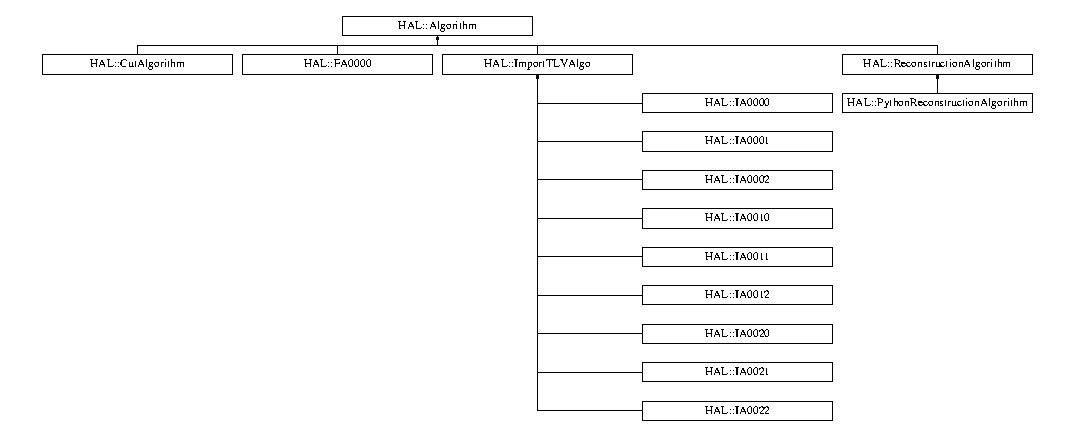
\includegraphics[height=12.000000cm]{class_h_a_l_1_1_algorithm}
\end{center}
\end{figure}
\subsection*{Public Member Functions}
\begin{DoxyCompactItemize}
\item 
\hypertarget{class_h_a_l_1_1_algorithm_a50506c07b5959ecd740f5683bf50ea93}{{\bfseries Algorithm} (T\+String name=\char`\"{}\char`\"{}, T\+String title=\char`\"{}\char`\"{})}\label{class_h_a_l_1_1_algorithm_a50506c07b5959ecd740f5683bf50ea93}

\item 
\hypertarget{class_h_a_l_1_1_algorithm_a77b66292cc2f8e021ed819daebbd7c51}{{\bfseries Algorithm} (const \hyperlink{class_h_a_l_1_1_algorithm}{Algorithm} \&algo)}\label{class_h_a_l_1_1_algorithm_a77b66292cc2f8e021ed819daebbd7c51}

\item 
\hypertarget{class_h_a_l_1_1_algorithm_a6e6834d936897cd573ce858d9b26150e}{void {\bfseries Add} (\hyperlink{class_h_a_l_1_1_algorithm}{Algorithm} $\ast$algo)}\label{class_h_a_l_1_1_algorithm_a6e6834d936897cd573ce858d9b26150e}

\item 
\hypertarget{class_h_a_l_1_1_algorithm_aaadc2f897f854c3808753fe8bdc88507}{void {\bfseries ls} ()}\label{class_h_a_l_1_1_algorithm_aaadc2f897f854c3808753fe8bdc88507}

\item 
\hypertarget{class_h_a_l_1_1_algorithm_ac6dda46e3df39cc169aaf95ced0507df}{void {\bfseries Counter\+Summary} ()}\label{class_h_a_l_1_1_algorithm_ac6dda46e3df39cc169aaf95ced0507df}

\item 
\hypertarget{class_h_a_l_1_1_algorithm_ae989038537a82ae182821bf32036a15b}{void {\bfseries Cut\+Report} ()}\label{class_h_a_l_1_1_algorithm_ae989038537a82ae182821bf32036a15b}

\item 
\hypertarget{class_h_a_l_1_1_algorithm_a5a25656c41939992b7a701f9f6c22476}{void {\bfseries Delete\+Algos} ()}\label{class_h_a_l_1_1_algorithm_a5a25656c41939992b7a701f9f6c22476}

\item 
\hypertarget{class_h_a_l_1_1_algorithm_a7815cd340c0800cd2b5567814bbcc40a}{void {\bfseries Set\+Name} (T\+String name)}\label{class_h_a_l_1_1_algorithm_a7815cd340c0800cd2b5567814bbcc40a}

\item 
\hypertarget{class_h_a_l_1_1_algorithm_aa225c7fa0c6fdef7a2807c3eaa225d83}{void {\bfseries Set\+Title} (T\+String title)}\label{class_h_a_l_1_1_algorithm_aa225c7fa0c6fdef7a2807c3eaa225d83}

\item 
\hypertarget{class_h_a_l_1_1_algorithm_ae30243bd1c0691a003d33ba6b02518cc}{void {\bfseries Set\+Output\+File\+Name} (T\+String filename)}\label{class_h_a_l_1_1_algorithm_ae30243bd1c0691a003d33ba6b02518cc}

\item 
\hypertarget{class_h_a_l_1_1_algorithm_a0b2b7e0a90824e7c2ed31fd8fc299d61}{void {\bfseries Abort} ()}\label{class_h_a_l_1_1_algorithm_a0b2b7e0a90824e7c2ed31fd8fc299d61}

\item 
\hypertarget{class_h_a_l_1_1_algorithm_a77516eeeffb62ed507616ddd006e023c}{void {\bfseries Clean\+Algos} ()}\label{class_h_a_l_1_1_algorithm_a77516eeeffb62ed507616ddd006e023c}

\item 
\hypertarget{class_h_a_l_1_1_algorithm_a64a01d69f068ef29f19057d9f4c1b172}{void {\bfseries Execute\+Algo} (Option\+\_\+t $\ast$option=\char`\"{}0\char`\"{})}\label{class_h_a_l_1_1_algorithm_a64a01d69f068ef29f19057d9f4c1b172}

\item 
\hypertarget{class_h_a_l_1_1_algorithm_aaf9d9ecdf99c327ec4de93cd5930d3c4}{void {\bfseries Execute\+Algos} (Option\+\_\+t $\ast$option)}\label{class_h_a_l_1_1_algorithm_aaf9d9ecdf99c327ec4de93cd5930d3c4}

\item 
\hypertarget{class_h_a_l_1_1_algorithm_aeb9b42850a64b3c25e7035e04c68a508}{void {\bfseries Initialize\+Algo} (Option\+\_\+t $\ast$option)}\label{class_h_a_l_1_1_algorithm_aeb9b42850a64b3c25e7035e04c68a508}

\item 
\hypertarget{class_h_a_l_1_1_algorithm_af988397097b2a83fae058744d3a909a6}{void {\bfseries Begin\+Algo} (Option\+\_\+t $\ast$option)}\label{class_h_a_l_1_1_algorithm_af988397097b2a83fae058744d3a909a6}

\item 
\hypertarget{class_h_a_l_1_1_algorithm_a82cc758128d3745ba8c91f38c4aa4d15}{void {\bfseries Slave\+Begin\+Algo} (Option\+\_\+t $\ast$option)}\label{class_h_a_l_1_1_algorithm_a82cc758128d3745ba8c91f38c4aa4d15}

\item 
\hypertarget{class_h_a_l_1_1_algorithm_a205e6c98e7b7dfca647edadaa1d159e8}{void {\bfseries Notify\+Algo} (Option\+\_\+t $\ast$option)}\label{class_h_a_l_1_1_algorithm_a205e6c98e7b7dfca647edadaa1d159e8}

\item 
\hypertarget{class_h_a_l_1_1_algorithm_ae9b629cebefe6ac8629dd6a2e66d05d6}{void {\bfseries Slave\+Terminate\+Algo} (Option\+\_\+t $\ast$option)}\label{class_h_a_l_1_1_algorithm_ae9b629cebefe6ac8629dd6a2e66d05d6}

\item 
\hypertarget{class_h_a_l_1_1_algorithm_a085a431010582d5040e51ef91e1140f1}{void {\bfseries Terminate\+Algo} (Option\+\_\+t $\ast$option)}\label{class_h_a_l_1_1_algorithm_a085a431010582d5040e51ef91e1140f1}

\item 
\hypertarget{class_h_a_l_1_1_algorithm_a7fd35cf6dc1962b58e48905b178c1747}{void {\bfseries Add\+Data} (T\+String name, T\+Object $\ast$obj)}\label{class_h_a_l_1_1_algorithm_a7fd35cf6dc1962b58e48905b178c1747}

\item 
\hypertarget{class_h_a_l_1_1_algorithm_ae9b228550b42524824f7119604df1add}{T\+Object $\ast$ {\bfseries Get\+Data} (T\+String name)}\label{class_h_a_l_1_1_algorithm_ae9b228550b42524824f7119604df1add}

\item 
\hypertarget{class_h_a_l_1_1_algorithm_a6609ea9ac6dbc42adb5b110a41201c9a}{Bool\+\_\+t {\bfseries Check\+Data} (T\+String name)}\label{class_h_a_l_1_1_algorithm_a6609ea9ac6dbc42adb5b110a41201c9a}

\item 
\hypertarget{class_h_a_l_1_1_algorithm_af0211270f880699c5a260754bbaa9640}{void {\bfseries Delete\+Data} (T\+String name)}\label{class_h_a_l_1_1_algorithm_af0211270f880699c5a260754bbaa9640}

\item 
\hypertarget{class_h_a_l_1_1_algorithm_aaae65cc70d75b35bbf4a4c987ee5fb46}{void {\bfseries Assign\+Data\+List} (T\+List $\ast$list)}\label{class_h_a_l_1_1_algorithm_aaae65cc70d75b35bbf4a4c987ee5fb46}

\item 
\hypertarget{class_h_a_l_1_1_algorithm_ae80d02cd08ddc48a82f217af77ffde20}{\hyperlink{class_h_a_l_1_1_analysis_tree_reader}{Analysis\+Tree\+Reader} $\ast$ {\bfseries Get\+Raw\+Data} ()}\label{class_h_a_l_1_1_algorithm_ae80d02cd08ddc48a82f217af77ffde20}

\item 
\hypertarget{class_h_a_l_1_1_algorithm_ae9b7d3532acfaed9b502bd462bd22c94}{\hyperlink{class_h_a_l_1_1_analysis_data}{Analysis\+Data} $\ast$ {\bfseries Get\+User\+Data} ()}\label{class_h_a_l_1_1_algorithm_ae9b7d3532acfaed9b502bd462bd22c94}

\item 
\hypertarget{class_h_a_l_1_1_algorithm_af6233cfbe13ce76207a98b12d4da6f16}{\hyperlink{class_h_a_l_1_1_analysis_tree_writer}{Analysis\+Tree\+Writer} $\ast$ {\bfseries Get\+User\+Output} ()}\label{class_h_a_l_1_1_algorithm_af6233cfbe13ce76207a98b12d4da6f16}

\item 
\hypertarget{class_h_a_l_1_1_algorithm_a0a3b6fa6eb3cf0063187c2b442f64ae8}{T\+String {\bfseries Get\+Name} ()}\label{class_h_a_l_1_1_algorithm_a0a3b6fa6eb3cf0063187c2b442f64ae8}

\item 
\hypertarget{class_h_a_l_1_1_algorithm_a9245bfda990ffdbde86cc56bcacd5b72}{T\+String {\bfseries Get\+Title} ()}\label{class_h_a_l_1_1_algorithm_a9245bfda990ffdbde86cc56bcacd5b72}

\item 
\hypertarget{class_h_a_l_1_1_algorithm_abcc3c96084def439a83bdeb0a86cb1ae}{T\+String {\bfseries Get\+Output\+File\+Name} ()}\label{class_h_a_l_1_1_algorithm_abcc3c96084def439a83bdeb0a86cb1ae}

\item 
\hypertarget{class_h_a_l_1_1_algorithm_ad5a29ecf5e77004fdd807352a15fc730}{void {\bfseries Increase\+Counter} (long long n=1)}\label{class_h_a_l_1_1_algorithm_ad5a29ecf5e77004fdd807352a15fc730}

\item 
\hypertarget{class_h_a_l_1_1_algorithm_ad155a2508e2329c4be12fbe5ec55734a}{long long {\bfseries Get\+Counter} ()}\label{class_h_a_l_1_1_algorithm_ad155a2508e2329c4be12fbe5ec55734a}

\end{DoxyCompactItemize}
\subsection*{Protected Member Functions}
\begin{DoxyCompactItemize}
\item 
\hypertarget{class_h_a_l_1_1_algorithm_a6273512af97092a7e50955cb69776d82}{virtual void {\bfseries Begin} (Option\+\_\+t $\ast$=\char`\"{}\char`\"{})}\label{class_h_a_l_1_1_algorithm_a6273512af97092a7e50955cb69776d82}

\item 
\hypertarget{class_h_a_l_1_1_algorithm_a468feb5807252729c62cce7db7d60b1d}{virtual void {\bfseries Slave\+Begin} (Option\+\_\+t $\ast$=\char`\"{}\char`\"{})}\label{class_h_a_l_1_1_algorithm_a468feb5807252729c62cce7db7d60b1d}

\item 
\hypertarget{class_h_a_l_1_1_algorithm_abe2da2ce6a2d3ccfb492d8afd1d07331}{virtual void {\bfseries Init} (Option\+\_\+t $\ast$=\char`\"{}\char`\"{})}\label{class_h_a_l_1_1_algorithm_abe2da2ce6a2d3ccfb492d8afd1d07331}

\item 
\hypertarget{class_h_a_l_1_1_algorithm_acbbfee57e6c71ab04047dca6636f2c4f}{virtual void {\bfseries Notify} (Option\+\_\+t $\ast$=\char`\"{}\char`\"{})}\label{class_h_a_l_1_1_algorithm_acbbfee57e6c71ab04047dca6636f2c4f}

\item 
\hypertarget{class_h_a_l_1_1_algorithm_a438c5c54698aa014b660474d08703bc2}{virtual void {\bfseries Exec} (Option\+\_\+t $\ast$=\char`\"{}\char`\"{})}\label{class_h_a_l_1_1_algorithm_a438c5c54698aa014b660474d08703bc2}

\item 
\hypertarget{class_h_a_l_1_1_algorithm_a2a26a5549e92efaa968763ac51e6758a}{virtual void {\bfseries Clear} (Option\+\_\+t $\ast$=\char`\"{}\char`\"{})}\label{class_h_a_l_1_1_algorithm_a2a26a5549e92efaa968763ac51e6758a}

\item 
\hypertarget{class_h_a_l_1_1_algorithm_a9735cc4d7ef34d440aff116c8dbf5cbb}{virtual void {\bfseries Slave\+Terminate} (Option\+\_\+t $\ast$=\char`\"{}\char`\"{})}\label{class_h_a_l_1_1_algorithm_a9735cc4d7ef34d440aff116c8dbf5cbb}

\item 
\hypertarget{class_h_a_l_1_1_algorithm_ab974f3b6336b7b1002c72c04ad2b59cb}{virtual void {\bfseries Terminate} (Option\+\_\+t $\ast$=\char`\"{}\char`\"{})}\label{class_h_a_l_1_1_algorithm_ab974f3b6336b7b1002c72c04ad2b59cb}

\end{DoxyCompactItemize}
\subsection*{Protected Attributes}
\begin{DoxyCompactItemize}
\item 
\hypertarget{class_h_a_l_1_1_algorithm_aacc4824bcc223fc86f0f57662393e56c}{T\+List $\ast$ {\bfseries f\+Data\+List}}\label{class_h_a_l_1_1_algorithm_aacc4824bcc223fc86f0f57662393e56c}

\item 
\hypertarget{class_h_a_l_1_1_algorithm_a15bbd1834a2413957b2946e051584d49}{T\+String {\bfseries f\+Algorithm\+Type}}\label{class_h_a_l_1_1_algorithm_a15bbd1834a2413957b2946e051584d49}

\item 
\hypertarget{class_h_a_l_1_1_algorithm_a91a834bebb25ccc2e4324fcaf51bf294}{long long {\bfseries f\+Counter}}\label{class_h_a_l_1_1_algorithm_a91a834bebb25ccc2e4324fcaf51bf294}

\end{DoxyCompactItemize}


The documentation for this class was generated from the following file\+:\begin{DoxyCompactItemize}
\item 
/\+Users/jhetherly/src/root\+\_\+\+H\+A\+L/include/\+H\+A\+L/Algorithm.\+h\end{DoxyCompactItemize}

\hypertarget{class_h_a_l_1_1_analysis}{\section{H\-A\-L\-:\-:Analysis Class Reference}
\label{class_h_a_l_1_1_analysis}\index{H\-A\-L\-::\-Analysis@{H\-A\-L\-::\-Analysis}}
}
\subsection*{Public Member Functions}
\begin{DoxyCompactItemize}
\item 
\hypertarget{class_h_a_l_1_1_analysis_ab95bfff098f6a9543d444078cef3be91}{{\bfseries Analysis} (T\-String name=\char`\"{}\char`\"{}, T\-String title=\char`\"{}\char`\"{}, T\-String tree\-Name=\char`\"{}\char`\"{})}\label{class_h_a_l_1_1_analysis_ab95bfff098f6a9543d444078cef3be91}

\item 
\hypertarget{class_h_a_l_1_1_analysis_ac7e8314701f2b10f684d3b795031299e}{void {\bfseries Add\-Reco\-Algo} (\hyperlink{class_h_a_l_1_1_algorithm}{Algorithm} $\ast$r)}\label{class_h_a_l_1_1_analysis_ac7e8314701f2b10f684d3b795031299e}

\item 
\hypertarget{class_h_a_l_1_1_analysis_a4cdeca8d55dbfcc19261baedca02e424}{void {\bfseries Add\-Cut\-Algo} (\hyperlink{class_h_a_l_1_1_algorithm}{Algorithm} $\ast$c)}\label{class_h_a_l_1_1_analysis_a4cdeca8d55dbfcc19261baedca02e424}

\item 
\hypertarget{class_h_a_l_1_1_analysis_af755ad7b542eb634144c99b1d142519c}{void {\bfseries Print\-Analysis\-Flow} ()}\label{class_h_a_l_1_1_analysis_af755ad7b542eb634144c99b1d142519c}

\item 
\hypertarget{class_h_a_l_1_1_analysis_a56e97ef132e10b2a5f96c71c5145127b}{void {\bfseries Set\-Tree\-Object\-Name} (T\-String name)}\label{class_h_a_l_1_1_analysis_a56e97ef132e10b2a5f96c71c5145127b}

\item 
\hypertarget{class_h_a_l_1_1_analysis_abcbdb0f6cad2060cf3f6bca7d0eb9ada}{void {\bfseries Set\-Analysis\-Name} (T\-String name)}\label{class_h_a_l_1_1_analysis_abcbdb0f6cad2060cf3f6bca7d0eb9ada}

\item 
\hypertarget{class_h_a_l_1_1_analysis_ab4ecf4f7c5c29027ac3eb3e3a2e3a780}{void {\bfseries Set\-Analysis\-Title} (T\-String title)}\label{class_h_a_l_1_1_analysis_ab4ecf4f7c5c29027ac3eb3e3a2e3a780}

\item 
\hypertarget{class_h_a_l_1_1_analysis_a540cf522be42290e16d6ac0c7dbff0ba}{Int\-\_\-t {\bfseries Add\-Files} (T\-String fnames, Long64\-\_\-t nentries=1234567890)}\label{class_h_a_l_1_1_analysis_a540cf522be42290e16d6ac0c7dbff0ba}

\item 
\hypertarget{class_h_a_l_1_1_analysis_af8fccc1f3c27d6402ecad559648b7ff0}{Int\-\_\-t {\bfseries Add\-Files} (T\-Chain $\ast$fchain)}\label{class_h_a_l_1_1_analysis_af8fccc1f3c27d6402ecad559648b7ff0}

\item 
\hypertarget{class_h_a_l_1_1_analysis_a9e6b12787599c0c36f576350e2e93b8d}{void {\bfseries Set\-Output\-File\-Name} (T\-String fname)}\label{class_h_a_l_1_1_analysis_a9e6b12787599c0c36f576350e2e93b8d}

\item 
\hypertarget{class_h_a_l_1_1_analysis_a50f84d17528b7ba7621c65696dd81e75}{void {\bfseries Set\-Output\-Tree\-Name} (T\-String tname)}\label{class_h_a_l_1_1_analysis_a50f84d17528b7ba7621c65696dd81e75}

\item 
\hypertarget{class_h_a_l_1_1_analysis_a6461758cc06f7a334a487d857172983a}{void {\bfseries Set\-Output\-Tree\-Description} (T\-String tdescription)}\label{class_h_a_l_1_1_analysis_a6461758cc06f7a334a487d857172983a}

\item 
\hypertarget{class_h_a_l_1_1_analysis_afccfbae795035cfe75578fa805aefa93}{void {\bfseries Print\-Tree} (Option\-\_\-t $\ast$option=\char`\"{}\char`\"{})}\label{class_h_a_l_1_1_analysis_afccfbae795035cfe75578fa805aefa93}

\item 
\hypertarget{class_h_a_l_1_1_analysis_a7c6603a4cc7b74591f5c0427f59023d5}{const char $\ast$ {\bfseries Get\-Leaf\-Type} (T\-String leafname)}\label{class_h_a_l_1_1_analysis_a7c6603a4cc7b74591f5c0427f59023d5}

\item 
\hypertarget{class_h_a_l_1_1_analysis_a8410426a53f7828270531f1ec56340b8}{const char $\ast$ {\bfseries Get\-Leaf\-Type} (T\-String branchname, T\-String leafname)}\label{class_h_a_l_1_1_analysis_a8410426a53f7828270531f1ec56340b8}

\item 
\hypertarget{class_h_a_l_1_1_analysis_a6e11fa65e712377587ed4b6a1a62c8aa}{void {\bfseries Map\-Branch} (T\-String branchname, T\-String nickname)}\label{class_h_a_l_1_1_analysis_a6e11fa65e712377587ed4b6a1a62c8aa}

\item 
\hypertarget{class_h_a_l_1_1_analysis_a4278a2e961076913371dec71da389701}{Long64\-\_\-t {\bfseries Process} (Option\-\_\-t $\ast$option=\char`\"{}\char`\"{}, Long64\-\_\-t nentries=1234567890, Long64\-\_\-t firstentry=0)}\label{class_h_a_l_1_1_analysis_a4278a2e961076913371dec71da389701}

\end{DoxyCompactItemize}


The documentation for this class was generated from the following file\-:\begin{DoxyCompactItemize}
\item 
/\-Users/jhetherly/src/root\-\_\-\-H\-A\-L/include/\-H\-A\-L/Analysis.\-h\end{DoxyCompactItemize}

\hypertarget{class_h_a_l_1_1_analysis_data}{\section{H\-A\-L\-:\-:Analysis\-Data Class Reference}
\label{class_h_a_l_1_1_analysis_data}\index{H\-A\-L\-::\-Analysis\-Data@{H\-A\-L\-::\-Analysis\-Data}}
}
Inheritance diagram for H\-A\-L\-:\-:Analysis\-Data\-:\begin{figure}[H]
\begin{center}
\leavevmode
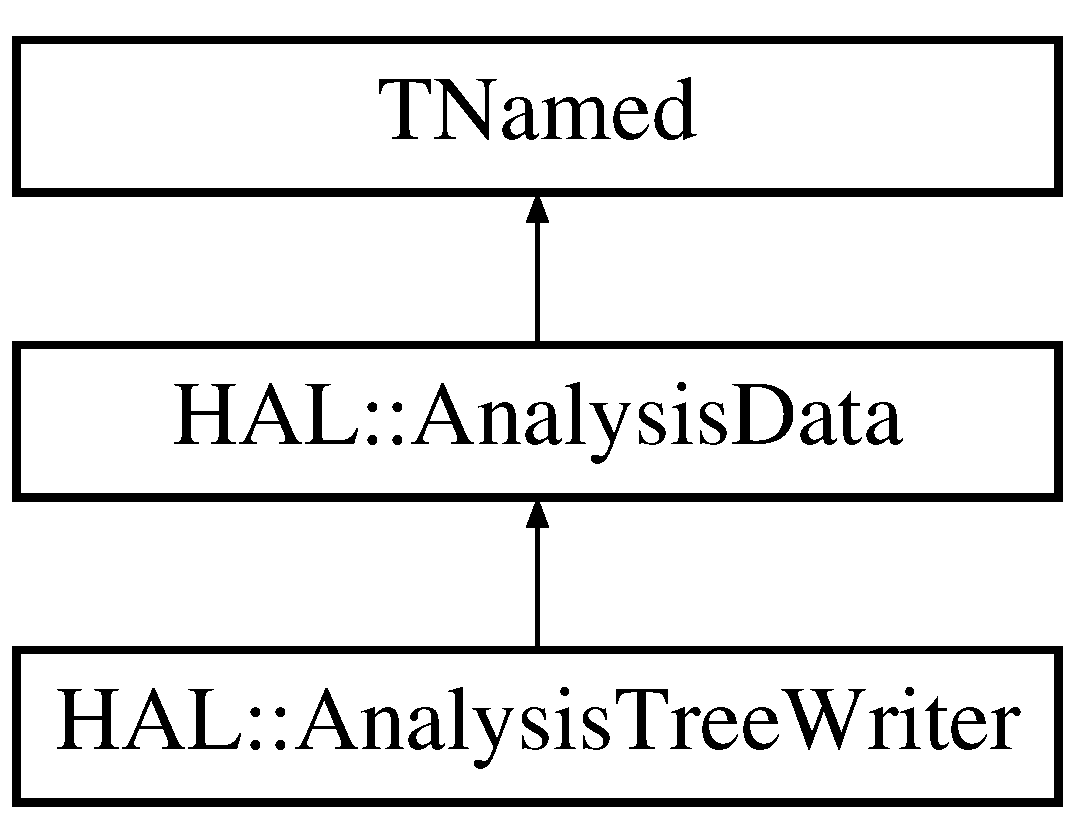
\includegraphics[height=3.000000cm]{class_h_a_l_1_1_analysis_data}
\end{center}
\end{figure}
\subsection*{Public Member Functions}
\begin{DoxyCompactItemize}
\item 
\hypertarget{class_h_a_l_1_1_analysis_data_a3870a72f6b39f3b4509b2498d285d94a}{virtual void {\bfseries Set\-Value} (const T\-String \&, const bool \&)}\label{class_h_a_l_1_1_analysis_data_a3870a72f6b39f3b4509b2498d285d94a}

\item 
\hypertarget{class_h_a_l_1_1_analysis_data_af74aff588a73f1c4d0a5e5ecbad14efb}{virtual void {\bfseries Set\-Value} (const T\-String \&, const long double \&)}\label{class_h_a_l_1_1_analysis_data_af74aff588a73f1c4d0a5e5ecbad14efb}

\item 
\hypertarget{class_h_a_l_1_1_analysis_data_ae88cc39a2594cf0bb969e3626cf17412}{virtual void {\bfseries Set\-Value} (const T\-String n, const double \&v)}\label{class_h_a_l_1_1_analysis_data_ae88cc39a2594cf0bb969e3626cf17412}

\item 
\hypertarget{class_h_a_l_1_1_analysis_data_a3953675a3b647f8c87eb214e25940d77}{virtual void {\bfseries Set\-Value} (const T\-String \&n, const float \&v)}\label{class_h_a_l_1_1_analysis_data_a3953675a3b647f8c87eb214e25940d77}

\item 
\hypertarget{class_h_a_l_1_1_analysis_data_ad18a729c4979bacc30d32e0802520236}{virtual void {\bfseries Set\-Value} (const T\-String \&, const long long \&)}\label{class_h_a_l_1_1_analysis_data_ad18a729c4979bacc30d32e0802520236}

\item 
\hypertarget{class_h_a_l_1_1_analysis_data_a2d3510dc4ee329387906e8738061b6b4}{virtual void {\bfseries Set\-Value} (const T\-String \&n, const short \&v)}\label{class_h_a_l_1_1_analysis_data_a2d3510dc4ee329387906e8738061b6b4}

\item 
\hypertarget{class_h_a_l_1_1_analysis_data_af8f2df54ad897dce65aa6224cac0af7c}{virtual void {\bfseries Set\-Value} (const T\-String \&n, const long \&v)}\label{class_h_a_l_1_1_analysis_data_af8f2df54ad897dce65aa6224cac0af7c}

\item 
\hypertarget{class_h_a_l_1_1_analysis_data_a697cb757197048cbcc5716bb32499c60}{virtual void {\bfseries Set\-Value} (const T\-String \&n, const int \&v)}\label{class_h_a_l_1_1_analysis_data_a697cb757197048cbcc5716bb32499c60}

\item 
\hypertarget{class_h_a_l_1_1_analysis_data_ae248b4f6c90034c9a41f8f8618ed89b8}{virtual void {\bfseries Set\-Value} (const T\-String \&n, const signed char \&v)}\label{class_h_a_l_1_1_analysis_data_ae248b4f6c90034c9a41f8f8618ed89b8}

\item 
\hypertarget{class_h_a_l_1_1_analysis_data_a0d21eebe0e1566531fa5c736f2cc6ed2}{virtual void {\bfseries Set\-Value} (const T\-String \&, const unsigned long long \&)}\label{class_h_a_l_1_1_analysis_data_a0d21eebe0e1566531fa5c736f2cc6ed2}

\item 
\hypertarget{class_h_a_l_1_1_analysis_data_a08be235fce5fd10cfafc592a2d9c1448}{virtual void {\bfseries Set\-Value} (const T\-String \&n, const unsigned short \&v)}\label{class_h_a_l_1_1_analysis_data_a08be235fce5fd10cfafc592a2d9c1448}

\item 
\hypertarget{class_h_a_l_1_1_analysis_data_af9cca2f941fef23004516aefc0d9c00d}{virtual void {\bfseries Set\-Value} (const T\-String \&n, const unsigned long \&v)}\label{class_h_a_l_1_1_analysis_data_af9cca2f941fef23004516aefc0d9c00d}

\item 
\hypertarget{class_h_a_l_1_1_analysis_data_adac44d46dc879cda67371131c18cf233}{virtual void {\bfseries Set\-Value} (const T\-String \&n, const unsigned int \&v)}\label{class_h_a_l_1_1_analysis_data_adac44d46dc879cda67371131c18cf233}

\item 
\hypertarget{class_h_a_l_1_1_analysis_data_ab3237d1010394bff323821642ea2380c}{virtual void {\bfseries Set\-Value} (const T\-String \&n, const unsigned char \&v)}\label{class_h_a_l_1_1_analysis_data_ab3237d1010394bff323821642ea2380c}

\item 
\hypertarget{class_h_a_l_1_1_analysis_data_a3fcb628c26524a1cc11db49295581d2d}{virtual void {\bfseries Set\-Value} (const T\-String \&n, const std\-::string \&v)}\label{class_h_a_l_1_1_analysis_data_a3fcb628c26524a1cc11db49295581d2d}

\item 
\hypertarget{class_h_a_l_1_1_analysis_data_acb8dd69db78b9d748ad4966584c7fa78}{virtual void {\bfseries Set\-Value} (const T\-String \&n, const T\-String \&v)}\label{class_h_a_l_1_1_analysis_data_acb8dd69db78b9d748ad4966584c7fa78}

\item 
\hypertarget{class_h_a_l_1_1_analysis_data_a7ffd3d35192f72eeadb3274a9bf8694d}{virtual void {\bfseries Set\-Value} (const T\-String \&n, const char \&v)}\label{class_h_a_l_1_1_analysis_data_a7ffd3d35192f72eeadb3274a9bf8694d}

\item 
\hypertarget{class_h_a_l_1_1_analysis_data_ac30be252a2ee9afe72db28b4cc2160da}{virtual void {\bfseries Set\-Value} (const T\-String \&, T\-Object $\ast$)}\label{class_h_a_l_1_1_analysis_data_ac30be252a2ee9afe72db28b4cc2160da}

\item 
\hypertarget{class_h_a_l_1_1_analysis_data_a12ad774235747ddc93efe315b22bf9e6}{virtual void {\bfseries Set\-Value} (const T\-String \&, const bool \&, const long long \&)}\label{class_h_a_l_1_1_analysis_data_a12ad774235747ddc93efe315b22bf9e6}

\item 
\hypertarget{class_h_a_l_1_1_analysis_data_a2628f2b892533b16f0a991bee3e0054b}{virtual void {\bfseries Set\-Value} (const T\-String \&, const long double \&, const long long \&)}\label{class_h_a_l_1_1_analysis_data_a2628f2b892533b16f0a991bee3e0054b}

\item 
\hypertarget{class_h_a_l_1_1_analysis_data_a59a7de41ba6832fb70f97b4c1e275fd3}{virtual void {\bfseries Set\-Value} (const T\-String \&n, const double \&v, const long long \&i)}\label{class_h_a_l_1_1_analysis_data_a59a7de41ba6832fb70f97b4c1e275fd3}

\item 
\hypertarget{class_h_a_l_1_1_analysis_data_a69059a19ae4a37a01eedfa98c537c487}{virtual void {\bfseries Set\-Value} (const T\-String \&n, const float \&v, const long long \&i)}\label{class_h_a_l_1_1_analysis_data_a69059a19ae4a37a01eedfa98c537c487}

\item 
\hypertarget{class_h_a_l_1_1_analysis_data_aad5a01dc8b2510bdcb47854a3cdaba0d}{virtual void {\bfseries Set\-Value} (const T\-String \&, const long long \&, const long long \&)}\label{class_h_a_l_1_1_analysis_data_aad5a01dc8b2510bdcb47854a3cdaba0d}

\item 
\hypertarget{class_h_a_l_1_1_analysis_data_adfb861d9e83e6880e54d11447b7047be}{virtual void {\bfseries Set\-Value} (const T\-String \&n, const short \&v, const long long \&i)}\label{class_h_a_l_1_1_analysis_data_adfb861d9e83e6880e54d11447b7047be}

\item 
\hypertarget{class_h_a_l_1_1_analysis_data_ac01b1d8a623777b81d5969d2b553a003}{virtual void {\bfseries Set\-Value} (const T\-String \&n, const long \&v, const long long \&i)}\label{class_h_a_l_1_1_analysis_data_ac01b1d8a623777b81d5969d2b553a003}

\item 
\hypertarget{class_h_a_l_1_1_analysis_data_aaddff4f1a41b2311b5f59a4eb4eb7a41}{virtual void {\bfseries Set\-Value} (const T\-String \&n, const int \&v, const long long \&i)}\label{class_h_a_l_1_1_analysis_data_aaddff4f1a41b2311b5f59a4eb4eb7a41}

\item 
\hypertarget{class_h_a_l_1_1_analysis_data_acea99cc8c68cf2a9d5f82da7e0d33202}{virtual void {\bfseries Set\-Value} (const T\-String \&n, const signed char \&v, const long long \&i)}\label{class_h_a_l_1_1_analysis_data_acea99cc8c68cf2a9d5f82da7e0d33202}

\item 
\hypertarget{class_h_a_l_1_1_analysis_data_a20938ad3fcd255b41f894e44b3e363f8}{virtual void {\bfseries Set\-Value} (const T\-String \&, const unsigned long long \&, const long long \&)}\label{class_h_a_l_1_1_analysis_data_a20938ad3fcd255b41f894e44b3e363f8}

\item 
\hypertarget{class_h_a_l_1_1_analysis_data_a8d61e54fe6022a58837468e1059a7e80}{virtual void {\bfseries Set\-Value} (const T\-String \&n, const unsigned short \&v, const long long \&i)}\label{class_h_a_l_1_1_analysis_data_a8d61e54fe6022a58837468e1059a7e80}

\item 
\hypertarget{class_h_a_l_1_1_analysis_data_a2af1428a8feebf6769cb30dd656d4b1e}{virtual void {\bfseries Set\-Value} (const T\-String \&n, const unsigned long \&v, const long long \&i)}\label{class_h_a_l_1_1_analysis_data_a2af1428a8feebf6769cb30dd656d4b1e}

\item 
\hypertarget{class_h_a_l_1_1_analysis_data_a446ed8d103e405b5028a9cebeae11bdf}{virtual void {\bfseries Set\-Value} (const T\-String \&n, const unsigned int \&v, const long long \&i)}\label{class_h_a_l_1_1_analysis_data_a446ed8d103e405b5028a9cebeae11bdf}

\item 
\hypertarget{class_h_a_l_1_1_analysis_data_af11d8522043ee9ddebea6beddfafdb1f}{virtual void {\bfseries Set\-Value} (const T\-String \&n, const unsigned char \&v, const long long \&i)}\label{class_h_a_l_1_1_analysis_data_af11d8522043ee9ddebea6beddfafdb1f}

\item 
\hypertarget{class_h_a_l_1_1_analysis_data_a2c1fe18ae83a39d8278630896e3b20cf}{virtual void {\bfseries Set\-Value} (const T\-String \&, const std\-::string \&, const long long \&)}\label{class_h_a_l_1_1_analysis_data_a2c1fe18ae83a39d8278630896e3b20cf}

\item 
\hypertarget{class_h_a_l_1_1_analysis_data_a985317d132d7c150e61f869db7fa8197}{virtual void {\bfseries Set\-Value} (const T\-String \&n, const T\-String \&v, const long long \&i)}\label{class_h_a_l_1_1_analysis_data_a985317d132d7c150e61f869db7fa8197}

\item 
\hypertarget{class_h_a_l_1_1_analysis_data_ae67a81418f6b826dd9b04f4c1e6f6f43}{virtual void {\bfseries Set\-Value} (const T\-String \&n, const char \&v, const long long \&i)}\label{class_h_a_l_1_1_analysis_data_ae67a81418f6b826dd9b04f4c1e6f6f43}

\item 
\hypertarget{class_h_a_l_1_1_analysis_data_adb01a8781d1c24a520bcc1b2518b64d2}{virtual void {\bfseries Set\-Value} (const T\-String \&, T\-Object $\ast$, const long long \&)}\label{class_h_a_l_1_1_analysis_data_adb01a8781d1c24a520bcc1b2518b64d2}

\item 
\hypertarget{class_h_a_l_1_1_analysis_data_a8d9a745e5e829f20b1e2e5fd5651b5cb}{virtual void {\bfseries Set\-Value} (const T\-String \&, const bool \&, const long long \&, const long long \&)}\label{class_h_a_l_1_1_analysis_data_a8d9a745e5e829f20b1e2e5fd5651b5cb}

\item 
\hypertarget{class_h_a_l_1_1_analysis_data_ad81a9423de201ecd3993c69c4cbefe6c}{virtual void {\bfseries Set\-Value} (const T\-String \&, const long double \&, const long long \&, const long long \&)}\label{class_h_a_l_1_1_analysis_data_ad81a9423de201ecd3993c69c4cbefe6c}

\item 
\hypertarget{class_h_a_l_1_1_analysis_data_a53d8939f8a64262857f13025f1f040da}{virtual void {\bfseries Set\-Value} (const T\-String \&n, const double \&v, const long long \&i, const long long \&j)}\label{class_h_a_l_1_1_analysis_data_a53d8939f8a64262857f13025f1f040da}

\item 
\hypertarget{class_h_a_l_1_1_analysis_data_a0089459ec31db3ea3c5dd974502ba651}{virtual void {\bfseries Set\-Value} (const T\-String \&n, const float \&v, const long long \&i, const long long \&j)}\label{class_h_a_l_1_1_analysis_data_a0089459ec31db3ea3c5dd974502ba651}

\item 
\hypertarget{class_h_a_l_1_1_analysis_data_a04aaec235f3100f4324bc502764fe00f}{virtual void {\bfseries Set\-Value} (const T\-String \&, const long long \&, const long long \&, const long long \&)}\label{class_h_a_l_1_1_analysis_data_a04aaec235f3100f4324bc502764fe00f}

\item 
\hypertarget{class_h_a_l_1_1_analysis_data_ad17c472ec1b6a6a0259c26bc5e1d68a9}{virtual void {\bfseries Set\-Value} (const T\-String \&n, const short \&v, const long long \&i, const long long \&j)}\label{class_h_a_l_1_1_analysis_data_ad17c472ec1b6a6a0259c26bc5e1d68a9}

\item 
\hypertarget{class_h_a_l_1_1_analysis_data_a4ab8550b85c33c0d04fcc381c845a5c4}{virtual void {\bfseries Set\-Value} (const T\-String \&n, const long \&v, const long long \&i, const long long \&j)}\label{class_h_a_l_1_1_analysis_data_a4ab8550b85c33c0d04fcc381c845a5c4}

\item 
\hypertarget{class_h_a_l_1_1_analysis_data_a9e7eea804e43369c4a4a8c3b1dacad37}{virtual void {\bfseries Set\-Value} (const T\-String \&n, const int \&v, const long long \&i, const long long \&j)}\label{class_h_a_l_1_1_analysis_data_a9e7eea804e43369c4a4a8c3b1dacad37}

\item 
\hypertarget{class_h_a_l_1_1_analysis_data_aebc6089b43396b0f19c1e06862be5448}{virtual void {\bfseries Set\-Value} (const T\-String \&n, const signed char \&v, const long long \&i, const long long \&j)}\label{class_h_a_l_1_1_analysis_data_aebc6089b43396b0f19c1e06862be5448}

\item 
\hypertarget{class_h_a_l_1_1_analysis_data_ae89756ae4ac0bf7cffbd22fbb54a2ec0}{virtual void {\bfseries Set\-Value} (const T\-String \&, const unsigned long long \&, const long long \&, const long long \&)}\label{class_h_a_l_1_1_analysis_data_ae89756ae4ac0bf7cffbd22fbb54a2ec0}

\item 
\hypertarget{class_h_a_l_1_1_analysis_data_a3f98354687b412c2fb8e84615211d314}{virtual void {\bfseries Set\-Value} (const T\-String \&n, const unsigned short \&v, const long long \&i, const long long \&j)}\label{class_h_a_l_1_1_analysis_data_a3f98354687b412c2fb8e84615211d314}

\item 
\hypertarget{class_h_a_l_1_1_analysis_data_af569db19521306fa14e85bd9d784a17f}{virtual void {\bfseries Set\-Value} (const T\-String \&n, const unsigned long \&v, const long long \&i, const long long \&j)}\label{class_h_a_l_1_1_analysis_data_af569db19521306fa14e85bd9d784a17f}

\item 
\hypertarget{class_h_a_l_1_1_analysis_data_a9c57d185dc584fdfb7f38b86e5f47f53}{virtual void {\bfseries Set\-Value} (const T\-String \&n, const unsigned int \&v, const long long \&i, const long long \&j)}\label{class_h_a_l_1_1_analysis_data_a9c57d185dc584fdfb7f38b86e5f47f53}

\item 
\hypertarget{class_h_a_l_1_1_analysis_data_a976258cc088753ba46ddad2b89bec07a}{virtual void {\bfseries Set\-Value} (const T\-String \&n, const unsigned char \&v, const long long \&i, const long long \&j)}\label{class_h_a_l_1_1_analysis_data_a976258cc088753ba46ddad2b89bec07a}

\item 
\hypertarget{class_h_a_l_1_1_analysis_data_a3782d0d87d85a96370d1c1b26523bc7e}{virtual void {\bfseries Set\-Value} (const T\-String \&, const std\-::string \&, const long long \&, const long long \&)}\label{class_h_a_l_1_1_analysis_data_a3782d0d87d85a96370d1c1b26523bc7e}

\item 
\hypertarget{class_h_a_l_1_1_analysis_data_a6cc252333af3e3c425ad4a184f286816}{virtual void {\bfseries Set\-Value} (const T\-String \&n, const T\-String \&v, const long long \&i, const long long \&j)}\label{class_h_a_l_1_1_analysis_data_a6cc252333af3e3c425ad4a184f286816}

\item 
\hypertarget{class_h_a_l_1_1_analysis_data_a7ce85e90fa181f17d72476422da24a48}{virtual void {\bfseries Set\-Value} (const T\-String \&n, const char \&v, const long long \&i, const long long \&j)}\label{class_h_a_l_1_1_analysis_data_a7ce85e90fa181f17d72476422da24a48}

\item 
\hypertarget{class_h_a_l_1_1_analysis_data_aedeeb6d1ff74a47232f5cb33edfbd88c}{virtual void {\bfseries Set\-Value} (const T\-String \&, T\-Object $\ast$, const long long \&, const long long \&)}\label{class_h_a_l_1_1_analysis_data_aedeeb6d1ff74a47232f5cb33edfbd88c}

\item 
\hypertarget{class_h_a_l_1_1_analysis_data_a281cfe7bf707071ac81004f415842f50}{bool {\bfseries Get\-Bool} (const T\-String \&, const long long \&i=-\/1, const long long \&j=-\/1)}\label{class_h_a_l_1_1_analysis_data_a281cfe7bf707071ac81004f415842f50}

\item 
\hypertarget{class_h_a_l_1_1_analysis_data_aab51c395613c253b5bdd019eb72a78dc}{long double {\bfseries Get\-Decimal} (const T\-String \&, const long long \&i=-\/1, const long long \&j=-\/1)}\label{class_h_a_l_1_1_analysis_data_aab51c395613c253b5bdd019eb72a78dc}

\item 
\hypertarget{class_h_a_l_1_1_analysis_data_a4695a073f8dc031fd3f0c0c2d6d4a64e}{long long {\bfseries Get\-Integer} (const T\-String \&, const long long \&i=-\/1, const long long \&j=-\/1)}\label{class_h_a_l_1_1_analysis_data_a4695a073f8dc031fd3f0c0c2d6d4a64e}

\item 
\hypertarget{class_h_a_l_1_1_analysis_data_af7d47f613b3745eae74b59e82d718b5b}{unsigned long long {\bfseries Get\-Counting} (const T\-String \&, const long long \&i=-\/1, const long long \&j=-\/1)}\label{class_h_a_l_1_1_analysis_data_af7d47f613b3745eae74b59e82d718b5b}

\item 
\hypertarget{class_h_a_l_1_1_analysis_data_a983d806a18f7d81bf7b0405375442e9d}{T\-String {\bfseries Get\-String} (const T\-String \&, const long long \&i=-\/1, const long long \&j=-\/1)}\label{class_h_a_l_1_1_analysis_data_a983d806a18f7d81bf7b0405375442e9d}

\item 
\hypertarget{class_h_a_l_1_1_analysis_data_af1d5b191d8ccec6fb120a7debee1a474}{T\-Object $\ast$ {\bfseries Get\-T\-Object} (const T\-String \&, const long long \&i=-\/1, const long long \&j=-\/1)}\label{class_h_a_l_1_1_analysis_data_af1d5b191d8ccec6fb120a7debee1a474}

\item 
\hypertarget{class_h_a_l_1_1_analysis_data_a88485900b08fc820b2021234699d72d9}{bool {\bfseries Exists} (const T\-String \&n, const long long \&i=-\/1, const long long \&j=-\/1)}\label{class_h_a_l_1_1_analysis_data_a88485900b08fc820b2021234699d72d9}

\item 
\hypertarget{class_h_a_l_1_1_analysis_data_a493762f931219f8a720d06a263a4ad23}{unsigned {\bfseries Type\-Dim} (std\-::string n)}\label{class_h_a_l_1_1_analysis_data_a493762f931219f8a720d06a263a4ad23}

\item 
\hypertarget{class_h_a_l_1_1_analysis_data_ab0c4af2c4db8ebe38fd883ed0a2c2a72}{unsigned {\bfseries Type\-Dim} (const T\-String \&n)}\label{class_h_a_l_1_1_analysis_data_ab0c4af2c4db8ebe38fd883ed0a2c2a72}

\item 
\hypertarget{class_h_a_l_1_1_analysis_data_ae12492f13299eabe287205392489a4c4}{std\-::vector$<$ T\-String $>$ {\bfseries Get\-Similar\-Names} (const T\-String \&n, unsigned min\-\_\-dim)}\label{class_h_a_l_1_1_analysis_data_ae12492f13299eabe287205392489a4c4}

\item 
\hypertarget{class_h_a_l_1_1_analysis_data_a02f185a0bb593efe8f1e1605a8db7212}{void {\bfseries Copy\-Values} (const T\-String \&from, const T\-String \&to)}\label{class_h_a_l_1_1_analysis_data_a02f185a0bb593efe8f1e1605a8db7212}

\item 
\hypertarget{class_h_a_l_1_1_analysis_data_a44bfe71b3f3c88ce664e6d7b3bd9b111}{void {\bfseries Swap\-Values} (const T\-String \&n, long long i, long long j)}\label{class_h_a_l_1_1_analysis_data_a44bfe71b3f3c88ce664e6d7b3bd9b111}

\item 
\hypertarget{class_h_a_l_1_1_analysis_data_add418841a62be11aad64044e7eda5ffb}{void {\bfseries Reset} ()}\label{class_h_a_l_1_1_analysis_data_add418841a62be11aad64044e7eda5ffb}

\item 
\hypertarget{class_h_a_l_1_1_analysis_data_a39276ed7623a74cf6468fa9a69079e07}{void {\bfseries Remove\-Name\-And\-Data} (const T\-String \&)}\label{class_h_a_l_1_1_analysis_data_a39276ed7623a74cf6468fa9a69079e07}

\item 
\hypertarget{class_h_a_l_1_1_analysis_data_a35cbc682e6090bf2540ac62de07db82f}{void {\bfseries Remove\-Data} (const T\-String \&)}\label{class_h_a_l_1_1_analysis_data_a35cbc682e6090bf2540ac62de07db82f}

\item 
\hypertarget{class_h_a_l_1_1_analysis_data_a9e60f6b78b29280597ac991cf378f4f3}{void {\bfseries Remove\-All\-Associated\-Data} (const T\-String \&)}\label{class_h_a_l_1_1_analysis_data_a9e60f6b78b29280597ac991cf378f4f3}

\item 
\hypertarget{class_h_a_l_1_1_analysis_data_a0d63364d678190ac69e46922ad445b8a}{{\bfseries Class\-Def\-N\-V} (\hyperlink{class_h_a_l_1_1_analysis_data}{Analysis\-Data}, 0)}\label{class_h_a_l_1_1_analysis_data_a0d63364d678190ac69e46922ad445b8a}

\end{DoxyCompactItemize}
\subsection*{Public Attributes}
\begin{DoxyCompactItemize}
\item 
\hypertarget{class_h_a_l_1_1_analysis_data_adc7232f1a112de23d2b557740422ec9f}{std\-::map$<$ std\-::string, bool, \\*
internal\-::string\-\_\-cmp $>$ {\bfseries f\-Bool\-Map}}\label{class_h_a_l_1_1_analysis_data_adc7232f1a112de23d2b557740422ec9f}

\item 
\hypertarget{class_h_a_l_1_1_analysis_data_a79170e31902d40d73d6838b816e74dc8}{std\-::map$<$ std\-::string, long \\*
double, internal\-::string\-\_\-cmp $>$ {\bfseries f\-Decimal\-Map}}\label{class_h_a_l_1_1_analysis_data_a79170e31902d40d73d6838b816e74dc8}

\item 
\hypertarget{class_h_a_l_1_1_analysis_data_a5487671b851b8ce89298d7f770ab8f34}{std\-::map$<$ std\-::string, long \\*
long, internal\-::string\-\_\-cmp $>$ {\bfseries f\-Integer\-Map}}\label{class_h_a_l_1_1_analysis_data_a5487671b851b8ce89298d7f770ab8f34}

\item 
\hypertarget{class_h_a_l_1_1_analysis_data_a6f29542f7f2cd7e7377c56ac54592dd5}{std\-::map$<$ std\-::string, \\*
unsigned long long, \\*
internal\-::string\-\_\-cmp $>$ {\bfseries f\-Counting\-Map}}\label{class_h_a_l_1_1_analysis_data_a6f29542f7f2cd7e7377c56ac54592dd5}

\item 
\hypertarget{class_h_a_l_1_1_analysis_data_a3256b3efc77655ba25cc34a6986c00d5}{std\-::map$<$ std\-::string, \\*
std\-::string, \\*
internal\-::string\-\_\-cmp $>$ {\bfseries f\-String\-Map}}\label{class_h_a_l_1_1_analysis_data_a3256b3efc77655ba25cc34a6986c00d5}

\item 
\hypertarget{class_h_a_l_1_1_analysis_data_a913d66198c57cc2bd9f0e3e5d904e33f}{std\-::map$<$ std\-::string, T\-Object \\*
$\ast$, internal\-::string\-\_\-cmp $>$ {\bfseries f\-T\-Object\-Map}}\label{class_h_a_l_1_1_analysis_data_a913d66198c57cc2bd9f0e3e5d904e33f}

\item 
\hypertarget{class_h_a_l_1_1_analysis_data_a61184b1f5c3fe3a707ca6636ae9e13b0}{std\-::map$<$ std\-::string, \\*
std\-::map$<$ long long, bool $>$\\*
, internal\-::string\-\_\-cmp $>$ {\bfseries f\-Bool\-Int\-Map}}\label{class_h_a_l_1_1_analysis_data_a61184b1f5c3fe3a707ca6636ae9e13b0}

\item 
\hypertarget{class_h_a_l_1_1_analysis_data_af0f5c30034eba37c74179ea605623317}{std\-::map$<$ std\-::string, \\*
std\-::map$<$ long long, long \\*
double $>$, internal\-::string\-\_\-cmp $>$ {\bfseries f\-Decimal\-Int\-Map}}\label{class_h_a_l_1_1_analysis_data_af0f5c30034eba37c74179ea605623317}

\item 
\hypertarget{class_h_a_l_1_1_analysis_data_a62e023cb60a954070f043edd7dd77f75}{std\-::map$<$ std\-::string, \\*
std\-::map$<$ long long, long long $>$\\*
, internal\-::string\-\_\-cmp $>$ {\bfseries f\-Integer\-Int\-Map}}\label{class_h_a_l_1_1_analysis_data_a62e023cb60a954070f043edd7dd77f75}

\item 
\hypertarget{class_h_a_l_1_1_analysis_data_aa4f71b630137b5723ded88314a9301a0}{std\-::map$<$ std\-::string, \\*
std\-::map$<$ long long, unsigned \\*
long long $>$\\*
, internal\-::string\-\_\-cmp $>$ {\bfseries f\-Counting\-Int\-Map}}\label{class_h_a_l_1_1_analysis_data_aa4f71b630137b5723ded88314a9301a0}

\item 
\hypertarget{class_h_a_l_1_1_analysis_data_a68da09e7d00969715c53c1286d480c27}{std\-::map$<$ std\-::string, \\*
std\-::map$<$ long long, \\*
std\-::string $>$\\*
, internal\-::string\-\_\-cmp $>$ {\bfseries f\-String\-Int\-Map}}\label{class_h_a_l_1_1_analysis_data_a68da09e7d00969715c53c1286d480c27}

\item 
\hypertarget{class_h_a_l_1_1_analysis_data_a30331566889aaa845bd3edd475211cfc}{std\-::map$<$ std\-::string, \\*
std\-::map$<$ long long, T\-Object $\ast$ $>$\\*
, internal\-::string\-\_\-cmp $>$ {\bfseries f\-T\-Object\-Int\-Map}}\label{class_h_a_l_1_1_analysis_data_a30331566889aaa845bd3edd475211cfc}

\item 
\hypertarget{class_h_a_l_1_1_analysis_data_a4d6c6e21427e94fe1a53f524cf0fbbc5}{std\-::map$<$ std\-::string, \\*
std\-::map$<$ long long, std\-::map\\*
$<$ long long, bool $>$\\*
 $>$, internal\-::string\-\_\-cmp $>$ {\bfseries f\-Bool\-Int\-Int\-Map}}\label{class_h_a_l_1_1_analysis_data_a4d6c6e21427e94fe1a53f524cf0fbbc5}

\item 
\hypertarget{class_h_a_l_1_1_analysis_data_a48a5faced1a93d3f912b95314b0eb9f2}{std\-::map$<$ std\-::string, \\*
std\-::map$<$ long long, std\-::map\\*
$<$ long long, long double $>$\\*
 $>$, internal\-::string\-\_\-cmp $>$ {\bfseries f\-Decimal\-Int\-Int\-Map}}\label{class_h_a_l_1_1_analysis_data_a48a5faced1a93d3f912b95314b0eb9f2}

\item 
\hypertarget{class_h_a_l_1_1_analysis_data_ae0a0427f6204ac11136c141f56a8bb03}{std\-::map$<$ std\-::string, \\*
std\-::map$<$ long long, std\-::map\\*
$<$ long long, long long $>$\\*
 $>$, internal\-::string\-\_\-cmp $>$ {\bfseries f\-Integer\-Int\-Int\-Map}}\label{class_h_a_l_1_1_analysis_data_ae0a0427f6204ac11136c141f56a8bb03}

\item 
\hypertarget{class_h_a_l_1_1_analysis_data_ad50906057dfe2e1cda6756218f549201}{std\-::map$<$ std\-::string, \\*
std\-::map$<$ long long, std\-::map\\*
$<$ long long, unsigned long \\*
long $>$ $>$, internal\-::string\-\_\-cmp $>$ {\bfseries f\-Counting\-Int\-Int\-Map}}\label{class_h_a_l_1_1_analysis_data_ad50906057dfe2e1cda6756218f549201}

\item 
\hypertarget{class_h_a_l_1_1_analysis_data_ac06bbfebb1b319a3b17407c3a5bc17c2}{std\-::map$<$ std\-::string, \\*
std\-::map$<$ long long, std\-::map\\*
$<$ long long, std\-::string $>$\\*
 $>$, internal\-::string\-\_\-cmp $>$ {\bfseries f\-String\-Int\-Int\-Map}}\label{class_h_a_l_1_1_analysis_data_ac06bbfebb1b319a3b17407c3a5bc17c2}

\item 
\hypertarget{class_h_a_l_1_1_analysis_data_ac743254719039aa3af1d33b6a2558499}{std\-::map$<$ std\-::string, \\*
std\-::map$<$ long long, std\-::map\\*
$<$ long long, T\-Object $\ast$ $>$\\*
 $>$, internal\-::string\-\_\-cmp $>$ {\bfseries f\-T\-Object\-Int\-Int\-Map}}\label{class_h_a_l_1_1_analysis_data_ac743254719039aa3af1d33b6a2558499}

\end{DoxyCompactItemize}


The documentation for this class was generated from the following file\-:\begin{DoxyCompactItemize}
\item 
/\-Users/jhetherly/src/root\-\_\-\-H\-A\-L/include/\-H\-A\-L/Analysis\-Data.\-h\end{DoxyCompactItemize}

\hypertarget{class_h_a_l_1_1_analysis_selector}{\section{H\+A\+L\+:\+:Analysis\+Selector Class Reference}
\label{class_h_a_l_1_1_analysis_selector}\index{H\+A\+L\+::\+Analysis\+Selector@{H\+A\+L\+::\+Analysis\+Selector}}
}
Inheritance diagram for H\+A\+L\+:\+:Analysis\+Selector\+:\begin{figure}[H]
\begin{center}
\leavevmode
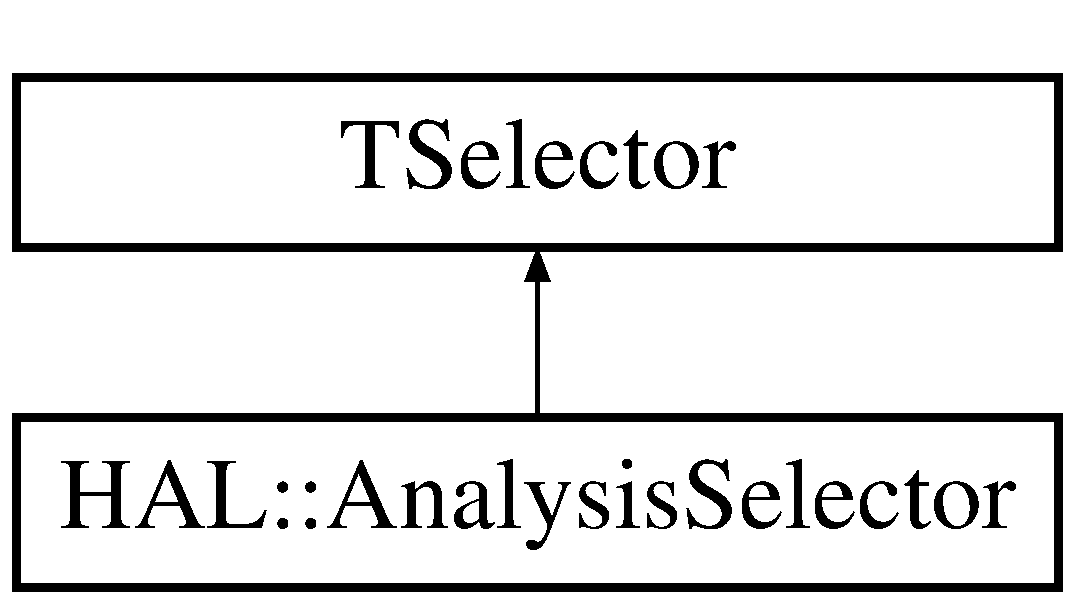
\includegraphics[height=2.000000cm]{class_h_a_l_1_1_analysis_selector}
\end{center}
\end{figure}
\subsection*{Public Member Functions}
\begin{DoxyCompactItemize}
\item 
\hypertarget{class_h_a_l_1_1_analysis_selector_a0e69d567472b846500e3758d0e1cafd3}{{\bfseries Analysis\+Selector} (\hyperlink{class_h_a_l_1_1_algorithm}{Algorithm} $\ast$af, T\+Tree $\ast$=0)}\label{class_h_a_l_1_1_analysis_selector_a0e69d567472b846500e3758d0e1cafd3}

\item 
\hypertarget{class_h_a_l_1_1_analysis_selector_a674eacd53bc6d9b2b82d5769ecf4c965}{virtual Int\+\_\+t {\bfseries Version} () const }\label{class_h_a_l_1_1_analysis_selector_a674eacd53bc6d9b2b82d5769ecf4c965}

\item 
\hypertarget{class_h_a_l_1_1_analysis_selector_aee810e2db449acf3c75cf0c7ed085318}{virtual void {\bfseries Begin} (T\+Tree $\ast$tree)}\label{class_h_a_l_1_1_analysis_selector_aee810e2db449acf3c75cf0c7ed085318}

\item 
\hypertarget{class_h_a_l_1_1_analysis_selector_a47feee7290d251295e65bc69b4e5b982}{virtual void {\bfseries Slave\+Begin} (T\+Tree $\ast$tree)}\label{class_h_a_l_1_1_analysis_selector_a47feee7290d251295e65bc69b4e5b982}

\item 
\hypertarget{class_h_a_l_1_1_analysis_selector_a73f70c38aab67b59e030bfa3e5182d3c}{virtual void {\bfseries Init} (T\+Tree $\ast$tree)}\label{class_h_a_l_1_1_analysis_selector_a73f70c38aab67b59e030bfa3e5182d3c}

\item 
\hypertarget{class_h_a_l_1_1_analysis_selector_a5ce023e4ee2bbc1d6ea0437175258195}{virtual Bool\+\_\+t {\bfseries Notify} ()}\label{class_h_a_l_1_1_analysis_selector_a5ce023e4ee2bbc1d6ea0437175258195}

\item 
\hypertarget{class_h_a_l_1_1_analysis_selector_ad89da1b73776f3acd5e8200d51438e47}{virtual Bool\+\_\+t {\bfseries Process} (Long64\+\_\+t entry)}\label{class_h_a_l_1_1_analysis_selector_ad89da1b73776f3acd5e8200d51438e47}

\item 
\hypertarget{class_h_a_l_1_1_analysis_selector_ae34c9fc9d657cea4c277306043997440}{virtual Int\+\_\+t {\bfseries Get\+Entry} (Long64\+\_\+t entry, Int\+\_\+t getall=0)}\label{class_h_a_l_1_1_analysis_selector_ae34c9fc9d657cea4c277306043997440}

\item 
\hypertarget{class_h_a_l_1_1_analysis_selector_a8e8f2ff599b95b4ea1437080f7a243e2}{virtual void {\bfseries Set\+Option} (const char $\ast$option)}\label{class_h_a_l_1_1_analysis_selector_a8e8f2ff599b95b4ea1437080f7a243e2}

\item 
\hypertarget{class_h_a_l_1_1_analysis_selector_a6c5b330612cbb40740a1773322f1bd4c}{virtual void {\bfseries Set\+Object} (T\+Object $\ast$obj)}\label{class_h_a_l_1_1_analysis_selector_a6c5b330612cbb40740a1773322f1bd4c}

\item 
\hypertarget{class_h_a_l_1_1_analysis_selector_a2ad21fe9c786a8b8ed9d2f2ed03b18dd}{virtual void {\bfseries Set\+Input\+List} (T\+List $\ast$input)}\label{class_h_a_l_1_1_analysis_selector_a2ad21fe9c786a8b8ed9d2f2ed03b18dd}

\item 
\hypertarget{class_h_a_l_1_1_analysis_selector_af839fdbf6d731039f3dfe2a28435cfa0}{virtual T\+List $\ast$ {\bfseries Get\+Output\+List} () const }\label{class_h_a_l_1_1_analysis_selector_af839fdbf6d731039f3dfe2a28435cfa0}

\item 
\hypertarget{class_h_a_l_1_1_analysis_selector_a83767cc68a8016682064a673b4cd3a81}{virtual void {\bfseries Slave\+Terminate} ()}\label{class_h_a_l_1_1_analysis_selector_a83767cc68a8016682064a673b4cd3a81}

\item 
\hypertarget{class_h_a_l_1_1_analysis_selector_a8b660b6a333cdefd12e1829389fbf0cd}{virtual void {\bfseries Terminate} ()}\label{class_h_a_l_1_1_analysis_selector_a8b660b6a333cdefd12e1829389fbf0cd}

\item 
\hypertarget{class_h_a_l_1_1_analysis_selector_a65b63a6f47a198031436edbea7818b1b}{void {\bfseries Set\+Output\+File\+Name} (T\+String fname)}\label{class_h_a_l_1_1_analysis_selector_a65b63a6f47a198031436edbea7818b1b}

\item 
\hypertarget{class_h_a_l_1_1_analysis_selector_a03cb0fb32fb595a20183a10651811a10}{void {\bfseries Set\+Output\+Tree\+Name} (T\+String tname)}\label{class_h_a_l_1_1_analysis_selector_a03cb0fb32fb595a20183a10651811a10}

\item 
\hypertarget{class_h_a_l_1_1_analysis_selector_ab1610526942d045e9bc1b2e4006575a5}{void {\bfseries Set\+Output\+Tree\+Description} (T\+String tdescription)}\label{class_h_a_l_1_1_analysis_selector_ab1610526942d045e9bc1b2e4006575a5}

\item 
\hypertarget{class_h_a_l_1_1_analysis_selector_a1e12ce6668b8f66ee0590dab7d9a6904}{void {\bfseries Set\+Message\+Period} (unsigned p=0)}\label{class_h_a_l_1_1_analysis_selector_a1e12ce6668b8f66ee0590dab7d9a6904}

\end{DoxyCompactItemize}
\subsection*{Public Attributes}
\begin{DoxyCompactItemize}
\item 
\hypertarget{class_h_a_l_1_1_analysis_selector_a7634b6d0eb916c352968a1a6acd7f3d2}{\hyperlink{class_h_a_l_1_1_algorithm}{Algorithm} $\ast$ {\bfseries f\+Analysis\+Flow}}\label{class_h_a_l_1_1_analysis_selector_a7634b6d0eb916c352968a1a6acd7f3d2}

\item 
\hypertarget{class_h_a_l_1_1_analysis_selector_a37f6980439f0b1e94db036220eacef8f}{T\+Tree $\ast$ {\bfseries f\+Chain}}\label{class_h_a_l_1_1_analysis_selector_a37f6980439f0b1e94db036220eacef8f}

\item 
\hypertarget{class_h_a_l_1_1_analysis_selector_a4d6e0e029b502012c4bf6d4f1618625c}{T\+Map $\ast$ \hyperlink{class_h_a_l_1_1_analysis_selector_a4d6e0e029b502012c4bf6d4f1618625c}{f\+Branch\+Map}}\label{class_h_a_l_1_1_analysis_selector_a4d6e0e029b502012c4bf6d4f1618625c}

\begin{DoxyCompactList}\small\item\em pointer to the analyzed T\+Tree or T\+Chain \end{DoxyCompactList}\end{DoxyCompactItemize}


The documentation for this class was generated from the following file\+:\begin{DoxyCompactItemize}
\item 
/\+Users/jhetherly/src/\+H\+A\+L-\/\+R\+O\+O\+T/include/\+H\+A\+L/Analysis\+Selector.\+h\end{DoxyCompactItemize}

\hypertarget{class_h_a_l_1_1_analysis_tree_reader}{\section{H\+A\+L\+:\+:Analysis\+Tree\+Reader Class Reference}
\label{class_h_a_l_1_1_analysis_tree_reader}\index{H\+A\+L\+::\+Analysis\+Tree\+Reader@{H\+A\+L\+::\+Analysis\+Tree\+Reader}}
}


Class for the easy extraction of data from a T\+Tree.  




{\ttfamily \#include $<$Analysis\+Tree\+Reader.\+h$>$}

Inheritance diagram for H\+A\+L\+:\+:Analysis\+Tree\+Reader\+:\begin{figure}[H]
\begin{center}
\leavevmode
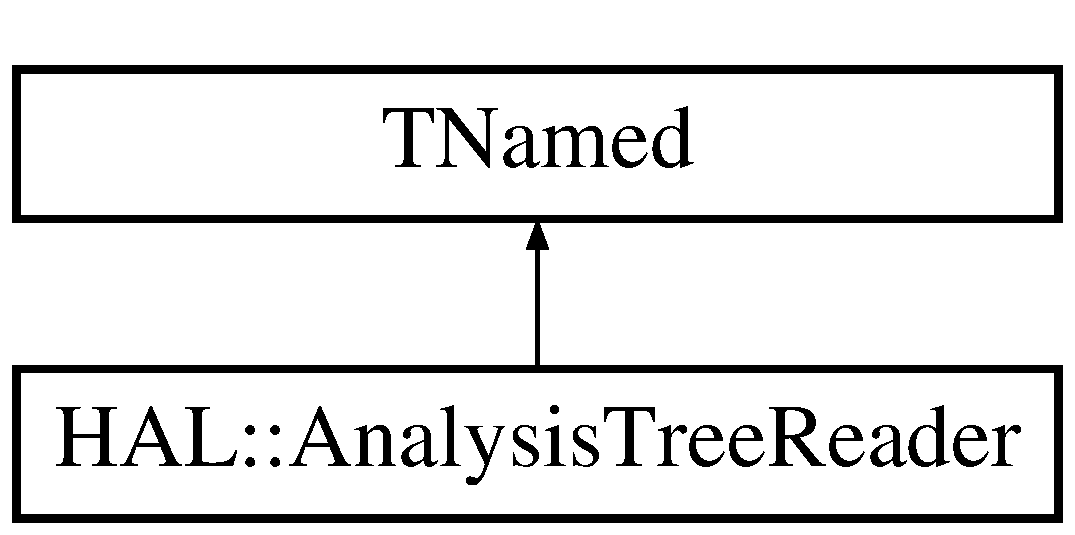
\includegraphics[height=2.000000cm]{class_h_a_l_1_1_analysis_tree_reader}
\end{center}
\end{figure}
\subsection*{Public Member Functions}
\begin{DoxyCompactItemize}
\item 
\hypertarget{class_h_a_l_1_1_analysis_tree_reader_ac00ba35d0b860566482e32c1dfd04827}{{\bfseries Analysis\+Tree\+Reader} (T\+Tree $\ast$tree=0)}\label{class_h_a_l_1_1_analysis_tree_reader_ac00ba35d0b860566482e32c1dfd04827}

\item 
\hypertarget{class_h_a_l_1_1_analysis_tree_reader_a031181c782d3620d271a92cef995d998}{void {\bfseries Set\+Tree} (T\+Tree $\ast$tree)}\label{class_h_a_l_1_1_analysis_tree_reader_a031181c782d3620d271a92cef995d998}

\item 
\hypertarget{class_h_a_l_1_1_analysis_tree_reader_a1a9c8bc30141df5fab1163f006fb08e3}{void {\bfseries Set\+Entry} (Long64\+\_\+t entry)}\label{class_h_a_l_1_1_analysis_tree_reader_a1a9c8bc30141df5fab1163f006fb08e3}

\item 
\hypertarget{class_h_a_l_1_1_analysis_tree_reader_a6fcf94a452ec53b66d9e0e49062d4e44}{Long64\+\_\+t {\bfseries Get\+Entry\+Number} ()}\label{class_h_a_l_1_1_analysis_tree_reader_a6fcf94a452ec53b66d9e0e49062d4e44}

\item 
\hypertarget{class_h_a_l_1_1_analysis_tree_reader_a6ad8933bd6c8cc2b17179c96fd3bfcb1}{T\+Tree $\ast$ {\bfseries Get\+Tree} ()}\label{class_h_a_l_1_1_analysis_tree_reader_a6ad8933bd6c8cc2b17179c96fd3bfcb1}

\item 
\hypertarget{class_h_a_l_1_1_analysis_tree_reader_a85f301e0ef78fdf1f239b36a030fb023}{T\+String {\bfseries Get\+Branch\+Name} (const T\+String \&name)}\label{class_h_a_l_1_1_analysis_tree_reader_a85f301e0ef78fdf1f239b36a030fb023}

\item 
\hypertarget{class_h_a_l_1_1_analysis_tree_reader_ab17ea6c10da56d9282d60d9507e01ef9}{void {\bfseries Init} ()}\label{class_h_a_l_1_1_analysis_tree_reader_ab17ea6c10da56d9282d60d9507e01ef9}

\item 
\hypertarget{class_h_a_l_1_1_analysis_tree_reader_adfe7aa4110b150fb1c7e80580a775a82}{Bool\+\_\+t {\bfseries Notify} ()}\label{class_h_a_l_1_1_analysis_tree_reader_adfe7aa4110b150fb1c7e80580a775a82}

\item 
\hypertarget{class_h_a_l_1_1_analysis_tree_reader_ae3dcc57b2cc27431e89edd341b300eb6}{void {\bfseries Set\+Branch\+Map} (T\+Map $\ast$m)}\label{class_h_a_l_1_1_analysis_tree_reader_ae3dcc57b2cc27431e89edd341b300eb6}

\item 
\hypertarget{class_h_a_l_1_1_analysis_tree_reader_afa371719adcfa583fe29ea0f468b9ea8}{bool {\bfseries Check\+Branch\+Map\+Nickname} (const T\+String \&name)}\label{class_h_a_l_1_1_analysis_tree_reader_afa371719adcfa583fe29ea0f468b9ea8}

\item 
\hypertarget{class_h_a_l_1_1_analysis_tree_reader_aa4dae5db1c660155760ded68007cdd6d}{unsigned int {\bfseries Get\+Rank} (const T\+String \&branchname)}\label{class_h_a_l_1_1_analysis_tree_reader_aa4dae5db1c660155760ded68007cdd6d}

\item 
\hypertarget{class_h_a_l_1_1_analysis_tree_reader_a1a8c741c6b2ae788b98d596c12543724}{unsigned int {\bfseries Get\+Dim} (const T\+String \&branchname, const long long \&idx\+\_\+1=-\/1)}\label{class_h_a_l_1_1_analysis_tree_reader_a1a8c741c6b2ae788b98d596c12543724}

\item 
\hypertarget{class_h_a_l_1_1_analysis_tree_reader_a8a76466f4746d4764b0fa97416182267}{bool {\bfseries Get\+Bool} (const T\+String \&branchname, const long long \&idx\+\_\+1=-\/1, const long long \&idx\+\_\+2=-\/1)}\label{class_h_a_l_1_1_analysis_tree_reader_a8a76466f4746d4764b0fa97416182267}

\item 
\hypertarget{class_h_a_l_1_1_analysis_tree_reader_a6b2e01f1075ed295513a268258d3d559}{long long {\bfseries Get\+Integer} (const T\+String \&branchname, const long long \&idx\+\_\+1=-\/1, const long long \&idx\+\_\+2=-\/1)}\label{class_h_a_l_1_1_analysis_tree_reader_a6b2e01f1075ed295513a268258d3d559}

\item 
\hypertarget{class_h_a_l_1_1_analysis_tree_reader_aa4d264484021ba0912f6254aeacc784f}{unsigned long long {\bfseries Get\+Counting} (const T\+String \&branchname, const long long \&idx\+\_\+1=-\/1, const long long \&idx\+\_\+2=-\/1)}\label{class_h_a_l_1_1_analysis_tree_reader_aa4d264484021ba0912f6254aeacc784f}

\item 
\hypertarget{class_h_a_l_1_1_analysis_tree_reader_a4a3dd2065768228ab817575307c4691e}{long double {\bfseries Get\+Decimal} (const T\+String \&branchname, const long long \&idx\+\_\+1=-\/1, const long long \&idx\+\_\+2=-\/1)}\label{class_h_a_l_1_1_analysis_tree_reader_a4a3dd2065768228ab817575307c4691e}

\item 
\hypertarget{class_h_a_l_1_1_analysis_tree_reader_a75c0fe7d907ac8f1792ff496e4cf0b73}{T\+String {\bfseries Get\+String} (const T\+String \&branchname, const long long \&idx\+\_\+1=-\/1, const long long \&idx\+\_\+2=-\/1)}\label{class_h_a_l_1_1_analysis_tree_reader_a75c0fe7d907ac8f1792ff496e4cf0b73}

\item 
\hypertarget{class_h_a_l_1_1_analysis_tree_reader_ad44870dd8478b8d404ede307726f2db6}{T\+Obj\+Array \& {\bfseries Get\+Obj\+Array} (const T\+String \&branchname, const long long \&idx\+\_\+1=-\/1)}\label{class_h_a_l_1_1_analysis_tree_reader_ad44870dd8478b8d404ede307726f2db6}

\item 
\hypertarget{class_h_a_l_1_1_analysis_tree_reader_ae9115ce6bba555009b6b21eca20339c9}{T\+Clones\+Array \& {\bfseries Get\+Clones\+Array} (const T\+String \&branchname, const long long \&idx\+\_\+1=-\/1)}\label{class_h_a_l_1_1_analysis_tree_reader_ae9115ce6bba555009b6b21eca20339c9}

\item 
\hypertarget{class_h_a_l_1_1_analysis_tree_reader_af010b9fafb8bd7f06efcaa46d1360253}{T\+Ref \& {\bfseries Get\+Ref} (const T\+String \&branchname, const long long \&idx\+\_\+1=-\/1, const long long \&idx\+\_\+2=-\/1)}\label{class_h_a_l_1_1_analysis_tree_reader_af010b9fafb8bd7f06efcaa46d1360253}

\item 
\hypertarget{class_h_a_l_1_1_analysis_tree_reader_a66bc43933f69938b94dd8caf5277395c}{T\+Ref\+Array \& {\bfseries Get\+Ref\+Array} (const T\+String \&branchname, const long long \&idx\+\_\+1=-\/1)}\label{class_h_a_l_1_1_analysis_tree_reader_a66bc43933f69938b94dd8caf5277395c}

\item 
\hypertarget{class_h_a_l_1_1_analysis_tree_reader_ad8be72de7b7f4ae5ced82c636ac91dd1}{{\bfseries Class\+Def} (\hyperlink{class_h_a_l_1_1_analysis_tree_reader}{Analysis\+Tree\+Reader}, 0)}\label{class_h_a_l_1_1_analysis_tree_reader_ad8be72de7b7f4ae5ced82c636ac91dd1}

\end{DoxyCompactItemize}
\subsection*{Friends}
\begin{DoxyCompactItemize}
\item 
\hypertarget{class_h_a_l_1_1_analysis_tree_reader_a3da00472573022c08436f19e0a48d8de}{class {\bfseries internal\+::\+Branch\+Manager}}\label{class_h_a_l_1_1_analysis_tree_reader_a3da00472573022c08436f19e0a48d8de}

\end{DoxyCompactItemize}


\subsection{Detailed Description}
Class for the easy extraction of data from a T\+Tree. 

This class allows for the easy retrieval of data stored in a T\+Tree. Through normal function calls the user can access data stored as scalars, C-\/arrays, S\+T\+L vectors, 2\+D C-\/arrays, and S\+T\+L vectors of vectors. A listing of the allowable types is given below. If a class that is stored in the T\+Tree can be decomposed in 'Make\+Class\+Mode,' this class can read it as well. The user should not need to worry about allocating memory or setting branch addresses. There are hard limits to the lengths of a C-\/array and 2\+D C-\/array that can be read. They are 10000 and 10000x100 respectively. If \hyperlink{namespace_h_a_l}{H\+A\+L} is compiled with R\+O\+O\+T version 6 or later, this restriction is lifted.~\newline
{\itshape Data Types That Can be Read\+:} \begin{TabularC}{6}
\hline
\rowcolor{lightgray}\PBS\centering {\bf Boolean }&\PBS\centering {\bf Integer }&\PBS\centering {\bf Counting }&\PBS\centering {\bf Decimal }&\PBS\centering {\bf String }&\PBS\centering {\bf Misc  }\\\cline{1-6}
\PBS\centering bool/\+Bool\+\_\+t &\PBS\centering int/\+Int\+\_\+t &\PBS\centering unsigned int/\+U\+Int\+\_\+t &\PBS\centering float/\+Float\+\_\+t/\+Float16\+\_\+t/\+Real\+\_\+t &\PBS\centering char/\+Char\+\_\+t/\+Text\+\_\+t &\PBS\centering T\+Obj\+Array \\\cline{1-6}
\PBS\centering &\PBS\centering short/\+Short\+\_\+t &\PBS\centering unsigned short/\+U\+Short\+\_\+t &\PBS\centering double/\+Double\+\_\+t/\+Double32\+\_\+t &\PBS\centering char$\ast$ &\PBS\centering T\+Clones\+Array \\\cline{1-6}
\PBS\centering &\PBS\centering long/\+Long\+\_\+t &\PBS\centering unsigned long/\+U\+Long\+\_\+t &\PBS\centering long double/\+Long\+Double\+\_\+t &\PBS\centering T\+String &\PBS\centering T\+Ref \\\cline{1-6}
\PBS\centering &\PBS\centering long long/\+Long64\+\_\+t &\PBS\centering unsigned long long/\+U\+Long64\+\_\+t &\PBS\centering &\PBS\centering T\+Obj\+String &\PBS\centering T\+Ref\+Array \\\cline{1-6}
\PBS\centering &\PBS\centering signed char &\PBS\centering unsigned char &\PBS\centering &\PBS\centering std\+::string &\PBS\centering T\+Ref\+Array \\\cline{1-6}
\end{TabularC}


The documentation for this class was generated from the following file\+:\begin{DoxyCompactItemize}
\item 
/\+Users/jhetherly/src/\+H\+A\+L-\/\+R\+O\+O\+T/include/\+H\+A\+L/\hyperlink{_analysis_tree_reader_8h}{Analysis\+Tree\+Reader.\+h}\end{DoxyCompactItemize}

\hypertarget{class_h_a_l_1_1_analysis_tree_writer}{\section{H\-A\-L\-:\-:Analysis\-Tree\-Writer Class Reference}
\label{class_h_a_l_1_1_analysis_tree_writer}\index{H\-A\-L\-::\-Analysis\-Tree\-Writer@{H\-A\-L\-::\-Analysis\-Tree\-Writer}}
}
Inheritance diagram for H\-A\-L\-:\-:Analysis\-Tree\-Writer\-:\begin{figure}[H]
\begin{center}
\leavevmode
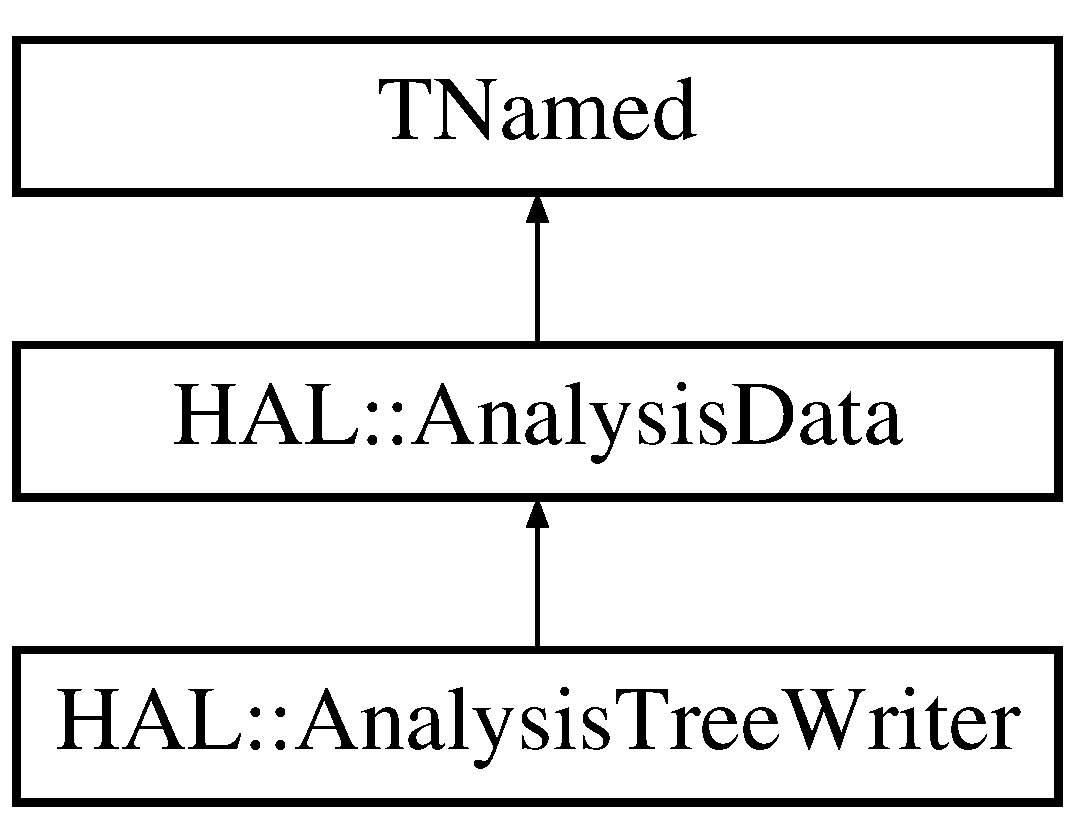
\includegraphics[height=3.000000cm]{class_h_a_l_1_1_analysis_tree_writer}
\end{center}
\end{figure}
\subsection*{Public Member Functions}
\begin{DoxyCompactItemize}
\item 
\hypertarget{class_h_a_l_1_1_analysis_tree_writer_a84bd5498078ffc6e67d5265b907705d5}{{\bfseries Analysis\-Tree\-Writer} (const T\-String \&ofile)}\label{class_h_a_l_1_1_analysis_tree_writer_a84bd5498078ffc6e67d5265b907705d5}

\item 
\hypertarget{class_h_a_l_1_1_analysis_tree_writer_a54d51c4078ebaeedd2ce02ac73945a78}{void {\bfseries Set\-Tree\-Name} (const T\-String \&tname)}\label{class_h_a_l_1_1_analysis_tree_writer_a54d51c4078ebaeedd2ce02ac73945a78}

\item 
\hypertarget{class_h_a_l_1_1_analysis_tree_writer_aec457c9a3f813a0ed455e1e4933ddb7f}{void {\bfseries Set\-Tree\-Description} (const T\-String \&tdescription)}\label{class_h_a_l_1_1_analysis_tree_writer_aec457c9a3f813a0ed455e1e4933ddb7f}

\item 
\hypertarget{class_h_a_l_1_1_analysis_tree_writer_a7e27d118b04eeba4c7fe66185c07434b}{void {\bfseries Set\-Tree\-For\-Branch} (const T\-String \&tree, const T\-String \&branch)}\label{class_h_a_l_1_1_analysis_tree_writer_a7e27d118b04eeba4c7fe66185c07434b}

\item 
\hypertarget{class_h_a_l_1_1_analysis_tree_writer_a91582d11e58a4b8d84d4ff35123a3ad3}{T\-String {\bfseries Get\-Tree\-For\-Branch} (const T\-String \&branch)}\label{class_h_a_l_1_1_analysis_tree_writer_a91582d11e58a4b8d84d4ff35123a3ad3}

\item 
\hypertarget{class_h_a_l_1_1_analysis_tree_writer_a2bc77354335ee48351205af7804356fc}{void {\bfseries Increment\-Count} ()}\label{class_h_a_l_1_1_analysis_tree_writer_a2bc77354335ee48351205af7804356fc}

\item 
\hypertarget{class_h_a_l_1_1_analysis_tree_writer_af49d85d3524d21a7da1a27d0a029239d}{void {\bfseries Write\-Data} ()}\label{class_h_a_l_1_1_analysis_tree_writer_af49d85d3524d21a7da1a27d0a029239d}

\item 
\hypertarget{class_h_a_l_1_1_analysis_tree_writer_af8dfdc6182004a8931d9c0f8926ae330}{virtual void {\bfseries Set\-Value} (const T\-String \&n, const bool \&v)}\label{class_h_a_l_1_1_analysis_tree_writer_af8dfdc6182004a8931d9c0f8926ae330}

\item 
\hypertarget{class_h_a_l_1_1_analysis_tree_writer_a85b8b7790bb9392ed1d865daab3248d7}{virtual void {\bfseries Set\-Value} (const T\-String \&n, const bool \&v, const long long \&i)}\label{class_h_a_l_1_1_analysis_tree_writer_a85b8b7790bb9392ed1d865daab3248d7}

\item 
\hypertarget{class_h_a_l_1_1_analysis_tree_writer_a2e68fdea10ca87aebab5332c2b680286}{virtual void {\bfseries Set\-Value} (const T\-String \&n, const long double \&v)}\label{class_h_a_l_1_1_analysis_tree_writer_a2e68fdea10ca87aebab5332c2b680286}

\item 
\hypertarget{class_h_a_l_1_1_analysis_tree_writer_ae4fbd939b2edfc2c3859ca24f635a475}{virtual void {\bfseries Set\-Value} (const T\-String \&n, const long double \&v, const long long \&i)}\label{class_h_a_l_1_1_analysis_tree_writer_ae4fbd939b2edfc2c3859ca24f635a475}

\item 
\hypertarget{class_h_a_l_1_1_analysis_tree_writer_a73bed978557c7222f4c88b71c1b74424}{virtual void {\bfseries Set\-Value} (const T\-String \&n, const long long \&v)}\label{class_h_a_l_1_1_analysis_tree_writer_a73bed978557c7222f4c88b71c1b74424}

\item 
\hypertarget{class_h_a_l_1_1_analysis_tree_writer_abc1b0d49980dfe48e99cf3c03f271bb3}{virtual void {\bfseries Set\-Value} (const T\-String \&n, const long long \&v, const long long \&i)}\label{class_h_a_l_1_1_analysis_tree_writer_abc1b0d49980dfe48e99cf3c03f271bb3}

\item 
\hypertarget{class_h_a_l_1_1_analysis_tree_writer_ad7fc39378d544f275cbb19145def8fbf}{virtual void {\bfseries Set\-Value} (const T\-String \&n, const unsigned long long \&v)}\label{class_h_a_l_1_1_analysis_tree_writer_ad7fc39378d544f275cbb19145def8fbf}

\item 
\hypertarget{class_h_a_l_1_1_analysis_tree_writer_ae71437812731ea60b3375c771ff912e1}{virtual void {\bfseries Set\-Value} (const T\-String \&n, const unsigned long long \&v, const long long \&i)}\label{class_h_a_l_1_1_analysis_tree_writer_ae71437812731ea60b3375c771ff912e1}

\item 
\hypertarget{class_h_a_l_1_1_analysis_tree_writer_a77da0342b01b89846c418b825d3a9d99}{{\bfseries Class\-Def\-N\-V} (\hyperlink{class_h_a_l_1_1_analysis_tree_writer}{Analysis\-Tree\-Writer}, 0)}\label{class_h_a_l_1_1_analysis_tree_writer_a77da0342b01b89846c418b825d3a9d99}

\end{DoxyCompactItemize}
\subsection*{Additional Inherited Members}


The documentation for this class was generated from the following file\-:\begin{DoxyCompactItemize}
\item 
/\-Users/jhetherly/src/root\-\_\-\-H\-A\-L/include/\-H\-A\-L/Analysis\-Tree\-Writer.\-h\end{DoxyCompactItemize}

\hypertarget{class_h_a_l_1_1_algorithms_1_1_attach_attribute}{\section{H\+A\+L\+:\+:Algorithms\+:\+:Attach\+Attribute Class Reference}
\label{class_h_a_l_1_1_algorithms_1_1_attach_attribute}\index{H\+A\+L\+::\+Algorithms\+::\+Attach\+Attribute@{H\+A\+L\+::\+Algorithms\+::\+Attach\+Attribute}}
}


Generic algorithm class that attaches a decimal value from a T\+Tree to an existing particle.  




{\ttfamily \#include $<$Algorithms.\+h$>$}

Inheritance diagram for H\+A\+L\+:\+:Algorithms\+:\+:Attach\+Attribute\+:\begin{figure}[H]
\begin{center}
\leavevmode
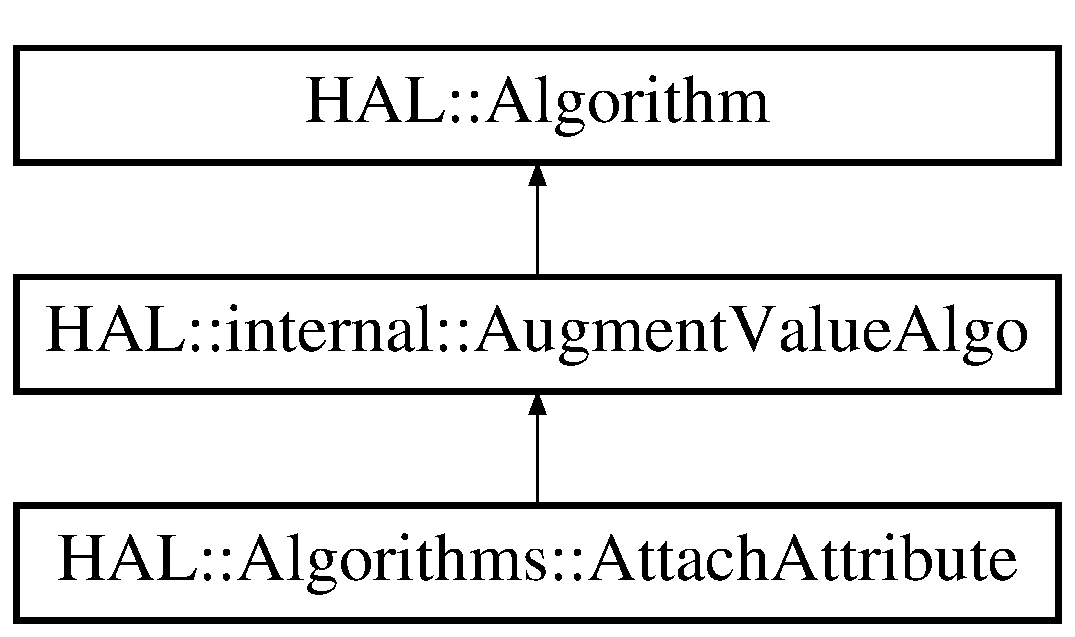
\includegraphics[height=3.000000cm]{class_h_a_l_1_1_algorithms_1_1_attach_attribute}
\end{center}
\end{figure}
\subsection*{Public Member Functions}
\begin{DoxyCompactItemize}
\item 
\hyperlink{class_h_a_l_1_1_algorithms_1_1_attach_attribute_a0c161228d7ba4e6b987d4d9d37375dde}{Attach\+Attribute} (T\+String name, T\+String title, T\+String input, T\+String attribute\+\_\+name)
\begin{DoxyCompactList}\small\item\em Constructor. \end{DoxyCompactList}\end{DoxyCompactItemize}
\subsection*{Protected Member Functions}
\begin{DoxyCompactItemize}
\item 
\hypertarget{class_h_a_l_1_1_algorithms_1_1_attach_attribute_afc87e37a8075b9486c1ec8b46c38b401}{virtual void {\bfseries Store\+Value} (\hyperlink{class_h_a_l_1_1_analysis_tree_reader}{H\+A\+L\+::\+Analysis\+Tree\+Reader} $\ast$, \hyperlink{class_h_a_l_1_1_generic_particle}{H\+A\+L\+::\+Particle\+Ptr}, long long)}\label{class_h_a_l_1_1_algorithms_1_1_attach_attribute_afc87e37a8075b9486c1ec8b46c38b401}

\end{DoxyCompactItemize}


\subsection{Detailed Description}
Generic algorithm class that attaches a decimal value from a T\+Tree to an existing particle. 

This algorithm imports the information to store a decimal value from a specified branch in a set of pre-\/existing particles. The input particles are irreversibly, non-\/destructively modified. This algorithm needs one branch map to locate the value to attach. The output from this algorithm may be accessed by either this algorithm's name or the name of the input algorithm.~\newline
~\newline
{\bfseries Explaination of the branch map\+:}~\newline
The required map is just one that points to the relavent value. $<$name$>$ refers to the name given to this algorithm's constructor.~\newline
{\itshape Required Branch Map\+:} \begin{TabularC}{2}
\hline
\rowcolor{lightgray}{\bf }&\PBS\centering {\bf Value  }\\\cline{1-2}
&\PBS\centering $<$name$>$\+:value \\\cline{1-2}
\end{TabularC}
{\bfseries Example\+:}~\newline
In your analysis file, do the following to attach charge to each muon (the easier way would be through \hyperlink{class_h_a_l_1_1_algorithms_1_1_import_particle}{Import\+Particle})\+:


\begin{DoxyCode}
\hyperlink{class_h_a_l_1_1_analysis}{HAL::Analysis} a(\textcolor{stringliteral}{"sample analysis"}, \textcolor{stringliteral}{""}, \textcolor{stringliteral}{"truth"});

a.AddAlgo(\textcolor{keyword}{new} \hyperlink{class_h_a_l_1_1_algorithms_1_1_import_particle}{HAL::Algorithms::ImportParticle}(\textcolor{stringliteral}{"muons"}, \textcolor{stringliteral}{"import basic muons"})
      );

a.AddAlgo(\textcolor{keyword}{new} \hyperlink{class_h_a_l_1_1_algorithms_1_1_attach_attribute}{HAL::Algorithms::AttachAttribute}(\textcolor{stringliteral}{"muon charge att"}, \textcolor{stringliteral}{"attach
       charge to muons"}, 
                                               \textcolor{stringliteral}{"muons"}, 
                                               \textcolor{stringliteral}{"muon charge"}));

\textcolor{comment}{//...}

a.MapBranch(\textcolor{stringliteral}{"mu\_charge"}, \textcolor{stringliteral}{"muon charge att:value"});
\end{DoxyCode}
 

\subsection{Constructor \& Destructor Documentation}
\hypertarget{class_h_a_l_1_1_algorithms_1_1_attach_attribute_a0c161228d7ba4e6b987d4d9d37375dde}{\index{H\+A\+L\+::\+Algorithms\+::\+Attach\+Attribute@{H\+A\+L\+::\+Algorithms\+::\+Attach\+Attribute}!Attach\+Attribute@{Attach\+Attribute}}
\index{Attach\+Attribute@{Attach\+Attribute}!H\+A\+L\+::\+Algorithms\+::\+Attach\+Attribute@{H\+A\+L\+::\+Algorithms\+::\+Attach\+Attribute}}
\subsubsection[{Attach\+Attribute}]{\setlength{\rightskip}{0pt plus 5cm}H\+A\+L\+::\+Algorithms\+::\+Attach\+Attribute\+::\+Attach\+Attribute (
\begin{DoxyParamCaption}
\item[{T\+String}]{name, }
\item[{T\+String}]{title, }
\item[{T\+String}]{input, }
\item[{T\+String}]{attribute\+\_\+name}
\end{DoxyParamCaption}
)\hspace{0.3cm}{\ttfamily [inline]}}}\label{class_h_a_l_1_1_algorithms_1_1_attach_attribute_a0c161228d7ba4e6b987d4d9d37375dde}


Constructor. 

Initializes the algorithm 
\begin{DoxyParams}[1]{Parameters}
\mbox{\tt in}  & {\em name} & Name of the algorithm. This can be used as the input to other algorithms. \\
\hline
\mbox{\tt in}  & {\em title} & Description of the algorithm. Can be an empty string. \\
\hline
\mbox{\tt in}  & {\em input} & Name of algorithm to attach values to. \\
\hline
\mbox{\tt in}  & {\em attribute\+\_\+name} & Name to give the attribute. \\
\hline
\end{DoxyParams}
\begin{DoxySeeAlso}{See also}
\hyperlink{class_h_a_l_1_1_algorithms_1_1_import_particle}{Import\+Particle}, \hyperlink{class_h_a_l_1_1_algorithms_1_1_select_particle}{Select\+Particle} 
\end{DoxySeeAlso}


The documentation for this class was generated from the following file\+:\begin{DoxyCompactItemize}
\item 
/\+Users/jhetherly/src/root\+\_\+\+H\+A\+L/include/\+H\+A\+L/\hyperlink{_algorithms_8h}{Algorithms.\+h}\end{DoxyCompactItemize}

\hypertarget{class_h_a_l_1_1_algorithms_1_1_cut}{\section{H\+A\+L\+:\+:Algorithms\+:\+:Cut Class Reference}
\label{class_h_a_l_1_1_algorithms_1_1_cut}\index{H\+A\+L\+::\+Algorithms\+::\+Cut@{H\+A\+L\+::\+Algorithms\+::\+Cut}}
}


Generic algorithm class that cuts on particle multiplicity, bool, integer, counting, and decimal values.  




{\ttfamily \#include $<$Algorithms.\+h$>$}

Inheritance diagram for H\+A\+L\+:\+:Algorithms\+:\+:Cut\+:\begin{figure}[H]
\begin{center}
\leavevmode
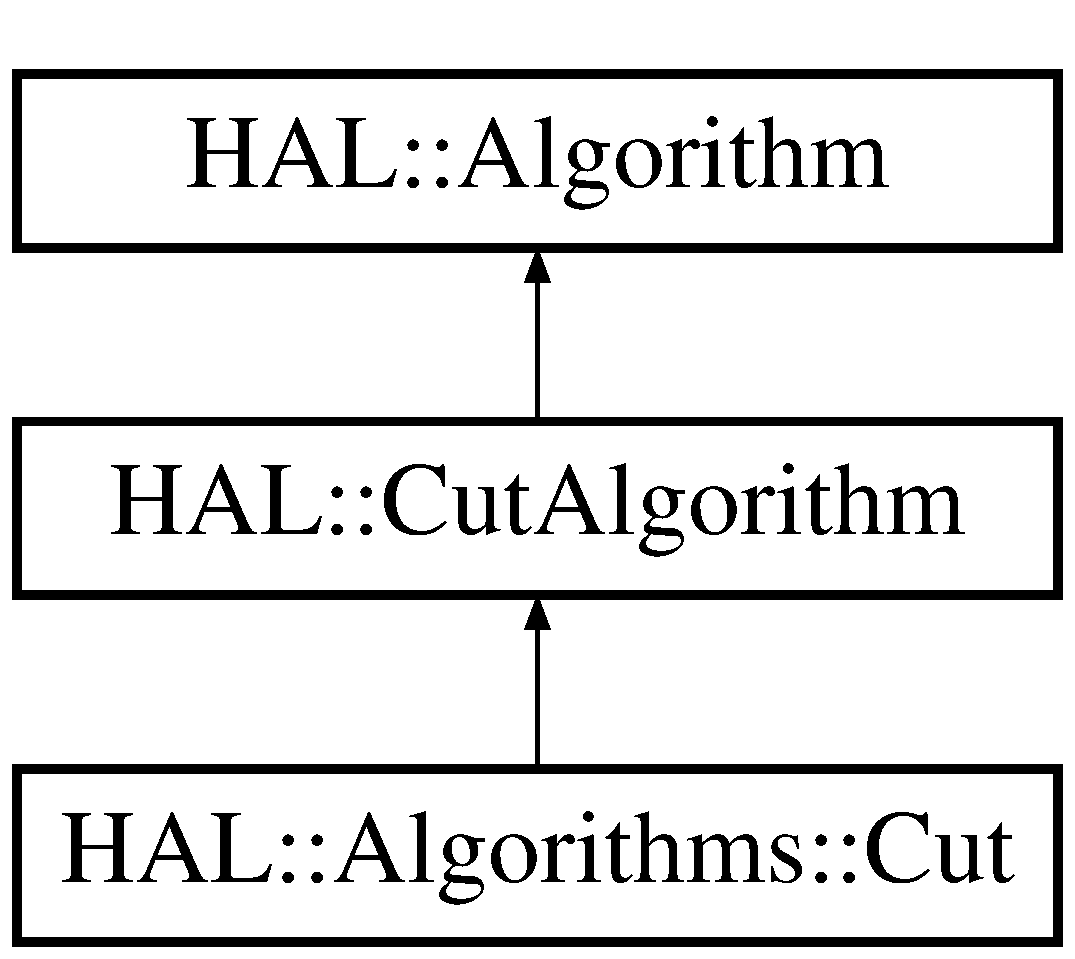
\includegraphics[height=3.000000cm]{class_h_a_l_1_1_algorithms_1_1_cut}
\end{center}
\end{figure}
\subsection*{Public Member Functions}
\begin{DoxyCompactItemize}
\item 
\hyperlink{class_h_a_l_1_1_algorithms_1_1_cut_a91f1ee2770d1a90d503cd1b6300dbce2}{Cut} (T\+String name, T\+String title, T\+String logic, long long ncuts,...)
\begin{DoxyCompactList}\small\item\em Constructor. \end{DoxyCompactList}\end{DoxyCompactItemize}
\subsection*{Protected Member Functions}
\begin{DoxyCompactItemize}
\item 
\hypertarget{class_h_a_l_1_1_algorithms_1_1_cut_aa1257616a4912852aa4ce2eb849e2ead}{virtual void {\bfseries Exec} (Option\+\_\+t $\ast$)}\label{class_h_a_l_1_1_algorithms_1_1_cut_aa1257616a4912852aa4ce2eb849e2ead}

\end{DoxyCompactItemize}
\subsection*{Additional Inherited Members}


\subsection{Detailed Description}
Generic algorithm class that cuts on particle multiplicity, bool, integer, counting, and decimal values. 

This algorithm provides a general mechanism to cut on several different algorithms. An important aspect of this algorithm is its ability to either \char`\"{}and\char`\"{} or \char`\"{}or\char`\"{} different predicates together. Combined with the proper selection algorithms, a cut on particle multiplicity is sufficient for most situations. The relational operators and types needed to specify a cut are listed below.~\newline
{\itshape Available Types of Cuts\+:} \begin{TabularC}{5}
\hline
\rowcolor{lightgray}\PBS\centering {\bf Boolean }&\PBS\centering {\bf Integer }&\PBS\centering {\bf Counting }&\PBS\centering {\bf Decimal }&\PBS\centering {\bf Particle Multiplicity  }\\\cline{1-5}
\PBS\centering bool &\PBS\centering integer &\PBS\centering counting &\PBS\centering decimal &\PBS\centering particle \\\cline{1-5}
\end{TabularC}
{\itshape Available Logical Relationships\+:} \begin{TabularC}{6}
\hline
\rowcolor{lightgray}\PBS\centering {\bf Equal }&\PBS\centering {\bf Not Equal }&\PBS\centering {\bf Greater Than }&\PBS\centering {\bf Greater Than or Equal To }&\PBS\centering {\bf Less Than }&\PBS\centering {\bf Less Than or Equal To  }\\\cline{1-6}
\PBS\centering == &\PBS\centering != &\PBS\centering $>$ &\PBS\centering $>$= &\PBS\centering $<$ &\PBS\centering $<$= \\\cline{1-6}
\end{TabularC}
{\itshape Note\+:} = may also be used in place of ==.~\newline
~\newline
{\bfseries Example\+:}~\newline
In your analysis file, do the following to create a cut\+:


\begin{DoxyCode}
\hyperlink{class_h_a_l_1_1_analysis}{HAL::Analysis} a(\textcolor{stringliteral}{"sample analysis"}, \textcolor{stringliteral}{""}, \textcolor{stringliteral}{"truth"});

\textcolor{comment}{//...}

a.AddAlgo(\textcolor{keyword}{new} \hyperlink{class_h_a_l_1_1_algorithms_1_1_import_particle}{HAL::Algorithms::ImportParticle}(\textcolor{stringliteral}{"jets"}, \textcolor{stringliteral}{"import basic jet
       objects"}));
a.AddAlgo(\textcolor{keyword}{new} \hyperlink{class_h_a_l_1_1_algorithms_1_1_import_particle}{HAL::Algorithms::ImportParticle}(\textcolor{stringliteral}{"mc"}, \textcolor{stringliteral}{"import basic Monte
       Carlo objects"}));

a.AddAlgo(\textcolor{keyword}{new} \hyperlink{class_h_a_l_1_1_algorithms_1_1_empty_cut}{HAL::Algorithms::EmptyCut}(\textcolor{stringliteral}{"number of events"}, \textcolor{stringliteral}{"baseline event number
      "}));

a.AddAlgo(\textcolor{keyword}{new} \hyperlink{class_h_a_l_1_1_algorithms_1_1_select_particle}{HAL::Algorithms::SelectParticle}(\textcolor{stringliteral}{"mc\_neutrinos"}, \textcolor{stringliteral}{"filter on mc
       id to get neutrinos"}, 
                                              \textcolor{stringliteral}{"mc"},
                                              \textcolor{stringliteral}{"id"}, 6,
                                              -16, -14, -12, 12, 14, 16));

a.AddAlgo(\textcolor{keyword}{new} \hyperlink{class_h_a_l_1_1_algorithms_1_1_particle_rank_selection}{HAL::Algorithms::ParticleRankSelection}(\textcolor{stringliteral}{"leading pt jet"}
      , \textcolor{stringliteral}{"find highest pt jet"}, 
                                                     \textcolor{stringliteral}{"jets"},
                                                     1, \textcolor{stringliteral}{"pt"}));
a.AddAlgo(\textcolor{keyword}{new} \hyperlink{class_h_a_l_1_1_algorithms_1_1_particle_rank_selection}{HAL::Algorithms::ParticleRankSelection}(\textcolor{stringliteral}{"subleading pt
       jet"}, \textcolor{stringliteral}{"find 2nd highest pt jet"}, 
                                                     \textcolor{stringliteral}{"jets"},
                                                     2, \textcolor{stringliteral}{"pt"}));

a.AddAlgo(\textcolor{keyword}{new} \hyperlink{class_h_a_l_1_1_algorithms_1_1_vec_add_reco}{HAL::Algorithms::VecAddReco}(\textcolor{stringliteral}{"di-jet"}, \textcolor{stringliteral}{"reconstruct a di-jet object
       from highest pt"}, 
                                          2, \textcolor{stringliteral}{"leading pt jet"}, \textcolor{stringliteral}{"subleading pt jet"}));

a.AddAlgo(\textcolor{keyword}{new} \hyperlink{class_h_a_l_1_1_algorithms_1_1_cut}{HAL::Algorithms::Cut}(\textcolor{stringliteral}{"di-jet and neutrino cut"}, \textcolor{stringliteral}{"make sure dijet and
       neutrino(s) exist"}, 
                                   \textcolor{stringliteral}{"and"}, 2,
                                   \textcolor{stringliteral}{"mc\_neutrinos"}, \textcolor{stringliteral}{"particle"}, \textcolor{stringliteral}{">="}, 1,
                                   \textcolor{stringliteral}{"di-jet"}, \textcolor{stringliteral}{"particle"}, \textcolor{stringliteral}{"=="}, 1));
\end{DoxyCode}
 

\subsection{Constructor \& Destructor Documentation}
\hypertarget{class_h_a_l_1_1_algorithms_1_1_cut_a91f1ee2770d1a90d503cd1b6300dbce2}{\index{H\+A\+L\+::\+Algorithms\+::\+Cut@{H\+A\+L\+::\+Algorithms\+::\+Cut}!Cut@{Cut}}
\index{Cut@{Cut}!H\+A\+L\+::\+Algorithms\+::\+Cut@{H\+A\+L\+::\+Algorithms\+::\+Cut}}
\subsubsection[{Cut}]{\setlength{\rightskip}{0pt plus 5cm}H\+A\+L\+::\+Algorithms\+::\+Cut\+::\+Cut (
\begin{DoxyParamCaption}
\item[{T\+String}]{name, }
\item[{T\+String}]{title, }
\item[{T\+String}]{logic, }
\item[{long long}]{ncuts, }
\item[{}]{...}
\end{DoxyParamCaption}
)}}\label{class_h_a_l_1_1_algorithms_1_1_cut_a91f1ee2770d1a90d503cd1b6300dbce2}


Constructor. 

Initializes the algorithm. The variable length argument at the end should conform to the following rules\+:~\newline

\begin{DoxyItemize}
\item It should be given in sets of four.
\item The first should be the name of the algorithm to cut
\item The second should be the type of cut
\item The third should be the relational operator
\item The fourth should be the value of the algorithm
\end{DoxyItemize}


\begin{DoxyParams}[1]{Parameters}
\mbox{\tt in}  & {\em name} & Name of the algorithm. This can be used as the input to other algorithms. \\
\hline
\mbox{\tt in}  & {\em title} & Description of the algorithm. Can be an empty string. \\
\hline
\mbox{\tt in}  & {\em logic} & Determines how to logically string together the cuts. Can be \char`\"{}and\char`\"{} or \char`\"{}or.\char`\"{} \\
\hline
\mbox{\tt in}  & {\em ncuts} & Number of cuts to make. \\
\hline
\mbox{\tt in}  & {\em ...} & Set of four values per cut as explained above. \\
\hline
\end{DoxyParams}
\begin{DoxySeeAlso}{See also}
\hyperlink{class_h_a_l_1_1_algorithms_1_1_empty_cut}{Empty\+Cut} 
\end{DoxySeeAlso}


The documentation for this class was generated from the following file\+:\begin{DoxyCompactItemize}
\item 
/\+Users/jhetherly/src/root\+\_\+\+H\+A\+L/include/\+H\+A\+L/\hyperlink{_algorithms_8h}{Algorithms.\+h}\end{DoxyCompactItemize}

\hypertarget{class_h_a_l_1_1_cut_algorithm}{\section{H\+A\+L\+:\+:Cut\+Algorithm Class Reference}
\label{class_h_a_l_1_1_cut_algorithm}\index{H\+A\+L\+::\+Cut\+Algorithm@{H\+A\+L\+::\+Cut\+Algorithm}}
}
Inheritance diagram for H\+A\+L\+:\+:Cut\+Algorithm\+:\begin{figure}[H]
\begin{center}
\leavevmode
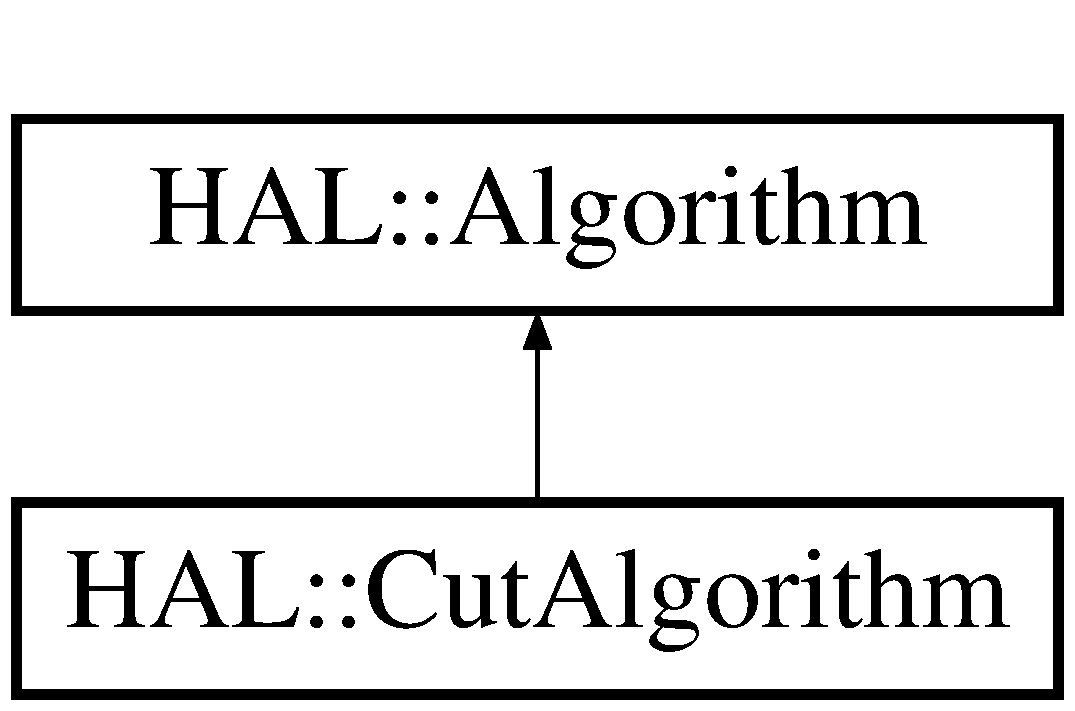
\includegraphics[height=3.000000cm]{class_h_a_l_1_1_cut_algorithm}
\end{center}
\end{figure}
\subsection*{Public Member Functions}
\begin{DoxyCompactItemize}
\item 
\hypertarget{class_h_a_l_1_1_cut_algorithm_a7009161a2b8463fddb9d6336cb2ef669}{{\bfseries Cut\+Algorithm} (T\+String name=\char`\"{}\char`\"{}, T\+String title=\char`\"{}\char`\"{})}\label{class_h_a_l_1_1_cut_algorithm_a7009161a2b8463fddb9d6336cb2ef669}

\end{DoxyCompactItemize}
\subsection*{Protected Member Functions}
\begin{DoxyCompactItemize}
\item 
\hypertarget{class_h_a_l_1_1_cut_algorithm_ad41a2ea5664562c3331f85bcc85317be}{void {\bfseries Passed} ()}\label{class_h_a_l_1_1_cut_algorithm_ad41a2ea5664562c3331f85bcc85317be}

\end{DoxyCompactItemize}
\subsection*{Additional Inherited Members}


The documentation for this class was generated from the following file\+:\begin{DoxyCompactItemize}
\item 
/\+Users/jhetherly/src/\+H\+A\+L-\/\+R\+O\+O\+T/include/\+H\+A\+L/Cut\+Algorithm.\+h\end{DoxyCompactItemize}

\hypertarget{class_h_a_l_1_1_cut_optimizer}{\section{H\+A\+L\+:\+:Cut\+Optimizer Class Reference}
\label{class_h_a_l_1_1_cut_optimizer}\index{H\+A\+L\+::\+Cut\+Optimizer@{H\+A\+L\+::\+Cut\+Optimizer}}
}
\subsection*{Public Member Functions}
\begin{DoxyCompactItemize}
\item 
\hypertarget{class_h_a_l_1_1_cut_optimizer_a7f1be065a4ec07a1e8cfee59dc0b80d1}{{\bfseries Cut\+Optimizer} (T\+F2 $\ast$st=N\+U\+L\+L)}\label{class_h_a_l_1_1_cut_optimizer_a7f1be065a4ec07a1e8cfee59dc0b80d1}

\item 
\hypertarget{class_h_a_l_1_1_cut_optimizer_a89082c3ec2719462ba90b3677119a1c6}{void {\bfseries Set\+Fitness\+Function} (T\+F2 $\ast$st=N\+U\+L\+L)}\label{class_h_a_l_1_1_cut_optimizer_a89082c3ec2719462ba90b3677119a1c6}

\item 
\hypertarget{class_h_a_l_1_1_cut_optimizer_a35eab754a13b06da0526fdf9900cc6eb}{T\+F2 $\ast$ {\bfseries Get\+Fitness\+Function} ()}\label{class_h_a_l_1_1_cut_optimizer_a35eab754a13b06da0526fdf9900cc6eb}

\item 
\hypertarget{class_h_a_l_1_1_cut_optimizer_a7055834b45ab96cbe30d335f7cd6f26d}{T\+Matrix\+D $\ast$ {\bfseries Optimize} (T\+H1 $\ast$sig, T\+H1 $\ast$bkg, Int\+\_\+t n, T\+String side=\char`\"{}both\char`\"{}, Int\+\_\+t rebin=1, Double\+\_\+t x\+\_\+min=T\+Math\+::\+Quiet\+Na\+N(), Double\+\_\+t x\+\_\+max=T\+Math\+::\+Quiet\+Na\+N())}\label{class_h_a_l_1_1_cut_optimizer_a7055834b45ab96cbe30d335f7cd6f26d}

\end{DoxyCompactItemize}


The documentation for this class was generated from the following file\+:\begin{DoxyCompactItemize}
\item 
/\+Users/jhetherly/src/\+H\+A\+L-\/\+R\+O\+O\+T/include/\+H\+A\+L/Cut\+Optimizer.\+h\end{DoxyCompactItemize}

\hypertarget{class_h_a_l_1_1_algorithms_1_1_empty_cut}{\section{H\-A\-L\-:\-:Algorithms\-:\-:Empty\-Cut Class Reference}
\label{class_h_a_l_1_1_algorithms_1_1_empty_cut}\index{H\-A\-L\-::\-Algorithms\-::\-Empty\-Cut@{H\-A\-L\-::\-Algorithms\-::\-Empty\-Cut}}
}


Generic algorithm class that serves as a baseline algorithm for any subsequent \hyperlink{class_h_a_l_1_1_algorithms_1_1_cut}{Cut} algorithms.  




{\ttfamily \#include $<$Algorithms.\-h$>$}

Inheritance diagram for H\-A\-L\-:\-:Algorithms\-:\-:Empty\-Cut\-:\begin{figure}[H]
\begin{center}
\leavevmode
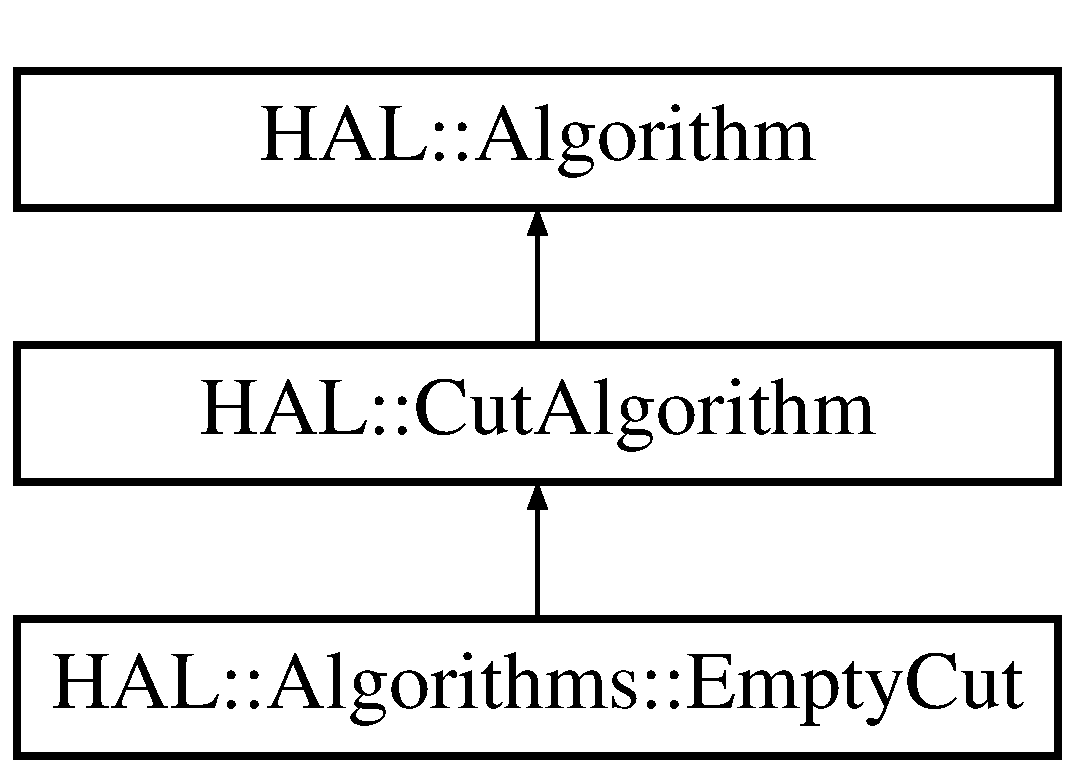
\includegraphics[height=3.000000cm]{class_h_a_l_1_1_algorithms_1_1_empty_cut}
\end{center}
\end{figure}
\subsection*{Public Member Functions}
\begin{DoxyCompactItemize}
\item 
\hyperlink{class_h_a_l_1_1_algorithms_1_1_empty_cut_a07eb3faf7e5ee7f913065cb01622cd8f}{Empty\-Cut} (T\-String name, T\-String title)
\begin{DoxyCompactList}\small\item\em Constructor. \end{DoxyCompactList}\end{DoxyCompactItemize}
\subsection*{Protected Member Functions}
\begin{DoxyCompactItemize}
\item 
\hypertarget{class_h_a_l_1_1_algorithms_1_1_empty_cut_a39235392c1b3a0f8253114dbcdf0a8a6}{virtual void {\bfseries Exec} (Option\-\_\-t $\ast$)}\label{class_h_a_l_1_1_algorithms_1_1_empty_cut_a39235392c1b3a0f8253114dbcdf0a8a6}

\end{DoxyCompactItemize}
\subsection*{Additional Inherited Members}


\subsection{Detailed Description}
Generic algorithm class that serves as a baseline algorithm for any subsequent \hyperlink{class_h_a_l_1_1_algorithms_1_1_cut}{Cut} algorithms. 

This algorithm passes all events. It can serve as a baseline cut in an analysis. {\bfseries Example\-:}\par
 In your analysis file, do the following to create a baseline cut\-:


\begin{DoxyCode}
\hyperlink{class_h_a_l_1_1_analysis}{HAL::Analysis} a(\textcolor{stringliteral}{"sample analysis"}, \textcolor{stringliteral}{""}, \textcolor{stringliteral}{"truth"});

a.AddAlgo(\textcolor{keyword}{new} \hyperlink{class_h_a_l_1_1_algorithms_1_1_empty_cut}{HAL::Algorithms::EmptyCut}(\textcolor{stringliteral}{"number of events"}, \textcolor{stringliteral}{"baseline event number
      "}));
\end{DoxyCode}
 

\subsection{Constructor \& Destructor Documentation}
\hypertarget{class_h_a_l_1_1_algorithms_1_1_empty_cut_a07eb3faf7e5ee7f913065cb01622cd8f}{\index{H\-A\-L\-::\-Algorithms\-::\-Empty\-Cut@{H\-A\-L\-::\-Algorithms\-::\-Empty\-Cut}!Empty\-Cut@{Empty\-Cut}}
\index{Empty\-Cut@{Empty\-Cut}!HAL::Algorithms::EmptyCut@{H\-A\-L\-::\-Algorithms\-::\-Empty\-Cut}}
\subsubsection[{Empty\-Cut}]{\setlength{\rightskip}{0pt plus 5cm}H\-A\-L\-::\-Algorithms\-::\-Empty\-Cut\-::\-Empty\-Cut (
\begin{DoxyParamCaption}
\item[{T\-String}]{name, }
\item[{T\-String}]{title}
\end{DoxyParamCaption}
)\hspace{0.3cm}{\ttfamily [inline]}}}\label{class_h_a_l_1_1_algorithms_1_1_empty_cut_a07eb3faf7e5ee7f913065cb01622cd8f}


Constructor. 

Initializes the algorithm 
\begin{DoxyParams}[1]{Parameters}
\mbox{\tt in}  & {\em name} & Name of the algorithm. This can be used as the input to other algorithms. \\
\hline
\mbox{\tt in}  & {\em title} & Description of the algorithm. Can be an empty string. \\
\hline
\end{DoxyParams}
\begin{DoxySeeAlso}{See Also}
\hyperlink{class_h_a_l_1_1_algorithms_1_1_cut}{Cut} 
\end{DoxySeeAlso}


The documentation for this class was generated from the following file\-:\begin{DoxyCompactItemize}
\item 
/\-Users/jhetherly/src/root\-\_\-\-H\-A\-L/include/\-H\-A\-L/\hyperlink{_algorithms_8h}{Algorithms.\-h}\end{DoxyCompactItemize}

\hypertarget{class_h_a_l_1_1_generic_data}{\section{H\-A\-L\-:\-:Generic\-Data Class Reference}
\label{class_h_a_l_1_1_generic_data}\index{H\-A\-L\-::\-Generic\-Data@{H\-A\-L\-::\-Generic\-Data}}
}
Inheritance diagram for H\-A\-L\-:\-:Generic\-Data\-:\begin{figure}[H]
\begin{center}
\leavevmode
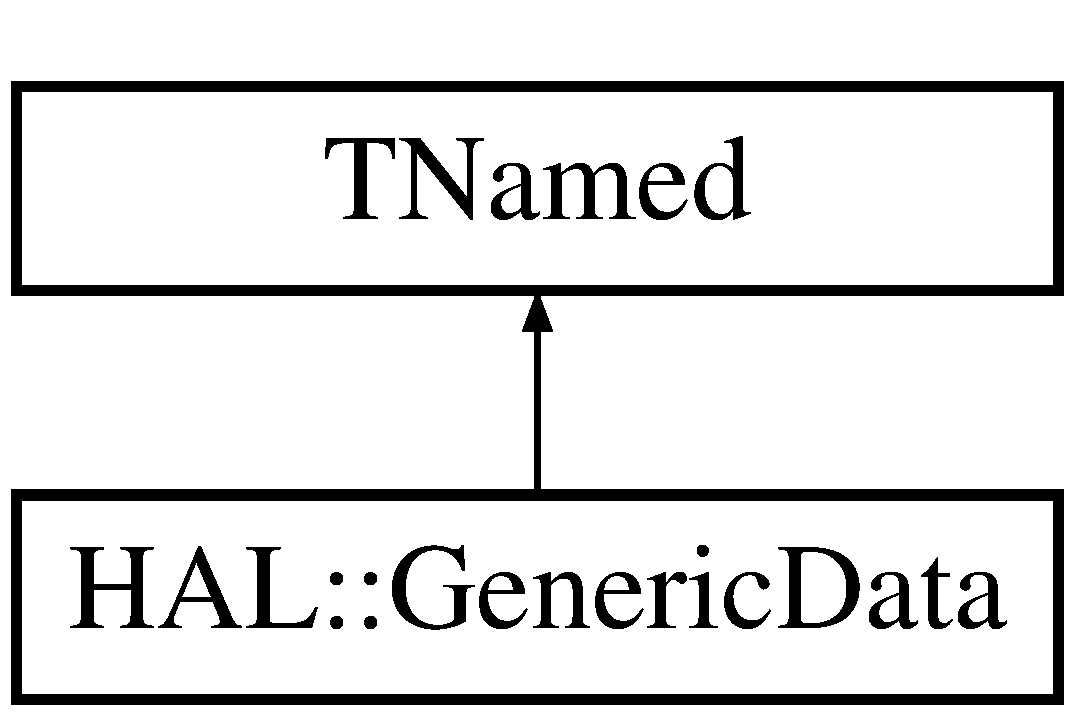
\includegraphics[height=2.000000cm]{class_h_a_l_1_1_generic_data}
\end{center}
\end{figure}
\subsection*{Public Member Functions}
\begin{DoxyCompactItemize}
\item 
\hypertarget{class_h_a_l_1_1_generic_data_ab2966008650b9dd6268688b26efac4ca}{{\bfseries Generic\-Data} (const T\-String \&name, bool is\-\_\-owner=false)}\label{class_h_a_l_1_1_generic_data_ab2966008650b9dd6268688b26efac4ca}

\item 
\hypertarget{class_h_a_l_1_1_generic_data_a0fc1d60fb890078bc42110602aad77a4}{{\bfseries Generic\-Data} (const \hyperlink{class_h_a_l_1_1_generic_data}{Generic\-Data} \&data)}\label{class_h_a_l_1_1_generic_data_a0fc1d60fb890078bc42110602aad77a4}

\item 
\hypertarget{class_h_a_l_1_1_generic_data_abbc23d840eb192ab59fb01645ae33d51}{void {\bfseries Set\-Ref\-Name} (const T\-String \&name)}\label{class_h_a_l_1_1_generic_data_abbc23d840eb192ab59fb01645ae33d51}

\item 
\hypertarget{class_h_a_l_1_1_generic_data_a3a19cd023aa97a81882f04e633fedbe5}{void {\bfseries Set\-Ref\-Type} (const T\-String \&type)}\label{class_h_a_l_1_1_generic_data_a3a19cd023aa97a81882f04e633fedbe5}

\item 
\hypertarget{class_h_a_l_1_1_generic_data_aca471249ad858ca39c41c66aa505ccb7}{void {\bfseries Add\-Particle} (\hyperlink{class_h_a_l_1_1_generic_particle}{Particle\-Ptr} particle)}\label{class_h_a_l_1_1_generic_data_aca471249ad858ca39c41c66aa505ccb7}

\item 
\hypertarget{class_h_a_l_1_1_generic_data_ac706724c448857289357f788eff350d7}{void {\bfseries Set\-Particles} (const T\-String \&name, Particle\-Ptrs \&particles)}\label{class_h_a_l_1_1_generic_data_ac706724c448857289357f788eff350d7}

\item 
\hypertarget{class_h_a_l_1_1_generic_data_a91b0d760e71de318a15b02bb8492035a}{T\-String {\bfseries Get\-Ref\-Name} ()}\label{class_h_a_l_1_1_generic_data_a91b0d760e71de318a15b02bb8492035a}

\item 
\hypertarget{class_h_a_l_1_1_generic_data_a4ed8d5cf423876674eddd941e5c93890}{T\-String {\bfseries Get\-Ref\-Type} ()}\label{class_h_a_l_1_1_generic_data_a4ed8d5cf423876674eddd941e5c93890}

\item 
\hypertarget{class_h_a_l_1_1_generic_data_a4956f4b4014bc1a7d32ad7399d622cba}{\hyperlink{class_h_a_l_1_1_generic_particle}{Particle\-Ptr} {\bfseries Get\-Particle} (const long long \&index)}\label{class_h_a_l_1_1_generic_data_a4956f4b4014bc1a7d32ad7399d622cba}

\item 
\hypertarget{class_h_a_l_1_1_generic_data_a601843b8bfda4d43a99cd46069b19d6c}{Particle\-Ptrs\-It {\bfseries Get\-Particle\-Begin} ()}\label{class_h_a_l_1_1_generic_data_a601843b8bfda4d43a99cd46069b19d6c}

\item 
\hypertarget{class_h_a_l_1_1_generic_data_a98b91768f0b886ac87611be8c7c490cd}{Particle\-Ptrs\-It {\bfseries Get\-Particle\-End} ()}\label{class_h_a_l_1_1_generic_data_a98b91768f0b886ac87611be8c7c490cd}

\item 
\hypertarget{class_h_a_l_1_1_generic_data_a88a50155c0cdc7dd76d681dcfb45dfc4}{Particle\-Ptrs \& {\bfseries Get\-Particles} (const T\-String \&name)}\label{class_h_a_l_1_1_generic_data_a88a50155c0cdc7dd76d681dcfb45dfc4}

\item 
\hypertarget{class_h_a_l_1_1_generic_data_a265c6f842139f2f7c8a12ff82962a15d}{bool {\bfseries Is\-Owner} ()}\label{class_h_a_l_1_1_generic_data_a265c6f842139f2f7c8a12ff82962a15d}

\item 
\hypertarget{class_h_a_l_1_1_generic_data_a444b2f7bd6c6e8ba6d585088f194928f}{T\-String {\bfseries Get\-Owner} ()}\label{class_h_a_l_1_1_generic_data_a444b2f7bd6c6e8ba6d585088f194928f}

\item 
\hypertarget{class_h_a_l_1_1_generic_data_a05638e168b83e998c8d1c1b58cfef9d2}{bool {\bfseries Has\-Particles} (const T\-String \&name)}\label{class_h_a_l_1_1_generic_data_a05638e168b83e998c8d1c1b58cfef9d2}

\item 
\hypertarget{class_h_a_l_1_1_generic_data_a521637ed1d84af87cf0ef5432893576f}{size\-\_\-t {\bfseries Get\-N\-Particles} ()}\label{class_h_a_l_1_1_generic_data_a521637ed1d84af87cf0ef5432893576f}

\item 
\hypertarget{class_h_a_l_1_1_generic_data_a0d2533aa45faf37a56b820f2b3a0d7d5}{size\-\_\-t {\bfseries Get\-N\-Particles} (const T\-String \&name)}\label{class_h_a_l_1_1_generic_data_a0d2533aa45faf37a56b820f2b3a0d7d5}

\item 
\hypertarget{class_h_a_l_1_1_generic_data_a737f93b6a0d228a7a7b8146cf6e151ea}{{\bfseries Class\-Def} (\hyperlink{class_h_a_l_1_1_generic_data}{Generic\-Data}, 0)}\label{class_h_a_l_1_1_generic_data_a737f93b6a0d228a7a7b8146cf6e151ea}

\end{DoxyCompactItemize}
\subsection*{Friends}
\begin{DoxyCompactItemize}
\item 
\hypertarget{class_h_a_l_1_1_generic_data_ad3342706941e18f58dc3a39a63ccfd7c}{std\-::ostream \& {\bfseries operator$<$$<$} (std\-::ostream \&os, \hyperlink{class_h_a_l_1_1_generic_data}{Generic\-Data} \&data)}\label{class_h_a_l_1_1_generic_data_ad3342706941e18f58dc3a39a63ccfd7c}

\end{DoxyCompactItemize}


The documentation for this class was generated from the following file\-:\begin{DoxyCompactItemize}
\item 
/\-Users/jhetherly/src/root\-\_\-\-H\-A\-L/include/\-H\-A\-L/Generic\-Data.\-h\end{DoxyCompactItemize}

\hypertarget{class_h_a_l_1_1_generic_particle}{\section{H\+A\+L\+:\+:Generic\+Particle Class Reference}
\label{class_h_a_l_1_1_generic_particle}\index{H\+A\+L\+::\+Generic\+Particle@{H\+A\+L\+::\+Generic\+Particle}}
}
Inheritance diagram for H\+A\+L\+:\+:Generic\+Particle\+:\begin{figure}[H]
\begin{center}
\leavevmode
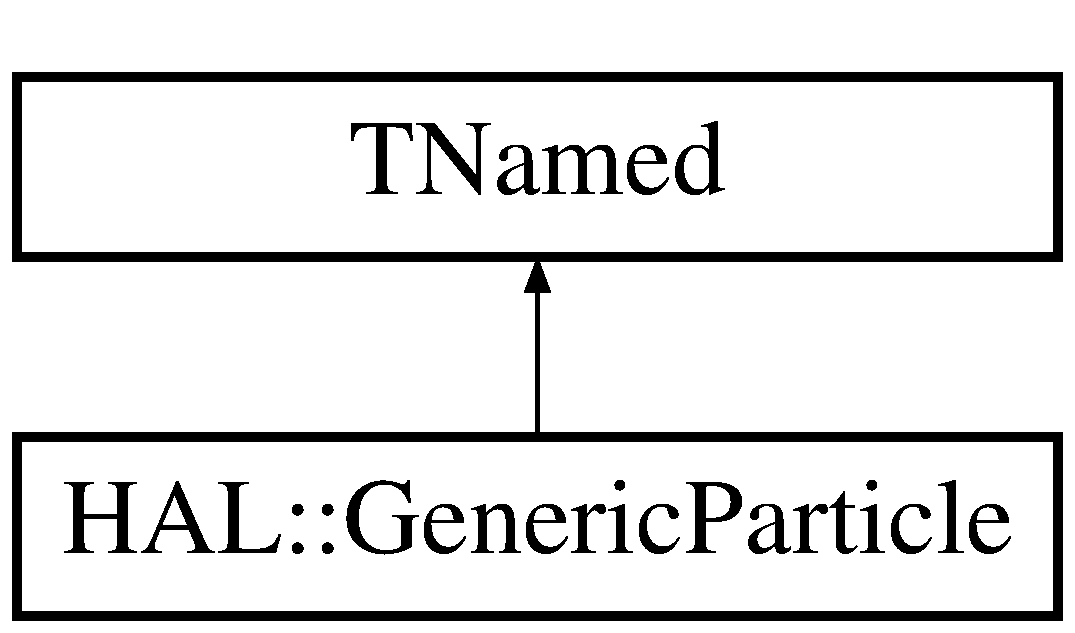
\includegraphics[height=2.000000cm]{class_h_a_l_1_1_generic_particle}
\end{center}
\end{figure}
\subsection*{Public Member Functions}
\begin{DoxyCompactItemize}
\item 
\hypertarget{class_h_a_l_1_1_generic_particle_add9ff51f2413528b2b00df1a4b7d67a5}{{\bfseries Generic\+Particle} (const T\+String \&owner, const T\+String \&origin=\char`\"{}\char`\"{}, const T\+String \&name=\char`\"{}\char`\"{})}\label{class_h_a_l_1_1_generic_particle_add9ff51f2413528b2b00df1a4b7d67a5}

\item 
\hypertarget{class_h_a_l_1_1_generic_particle_a1e9e01f96e31e980b2c31af42bb1c514}{{\bfseries Generic\+Particle} (const \hyperlink{class_h_a_l_1_1_generic_particle}{Generic\+Particle} \&particle)}\label{class_h_a_l_1_1_generic_particle_a1e9e01f96e31e980b2c31af42bb1c514}

\item 
\hypertarget{class_h_a_l_1_1_generic_particle_aca5a97bce5a002bd84259a417965f96e}{void {\bfseries Set\+Owner} (const T\+String \&owner)}\label{class_h_a_l_1_1_generic_particle_aca5a97bce5a002bd84259a417965f96e}

\item 
\hypertarget{class_h_a_l_1_1_generic_particle_a91b82bc5204850ab0d40163ed103ee12}{void {\bfseries Set\+Origin} (const T\+String \&origin)}\label{class_h_a_l_1_1_generic_particle_a91b82bc5204850ab0d40163ed103ee12}

\item 
\hypertarget{class_h_a_l_1_1_generic_particle_ae752a3a3a41281887a2ee988957cc6d9}{void {\bfseries Set\+Owner\+Index} (const size\+\_\+t \&oi)}\label{class_h_a_l_1_1_generic_particle_ae752a3a3a41281887a2ee988957cc6d9}

\item 
\hypertarget{class_h_a_l_1_1_generic_particle_a81d7aa1fd86d8f1d7e78286f32840e90}{void {\bfseries Set\+Origin\+Index} (const size\+\_\+t \&oi)}\label{class_h_a_l_1_1_generic_particle_a81d7aa1fd86d8f1d7e78286f32840e90}

\item 
\hypertarget{class_h_a_l_1_1_generic_particle_aa125325fe47360c75036732b90ca2c5b}{void {\bfseries Set\+I\+D} (const int \&id)}\label{class_h_a_l_1_1_generic_particle_aa125325fe47360c75036732b90ca2c5b}

\item 
\hypertarget{class_h_a_l_1_1_generic_particle_a06e76eefefa12e67947c8e3cfd0ab401}{void {\bfseries Set\+Charge} (const float \&charge)}\label{class_h_a_l_1_1_generic_particle_a06e76eefefa12e67947c8e3cfd0ab401}

\item 
\hypertarget{class_h_a_l_1_1_generic_particle_a985b92b525a1b6c2199b3c797dae153d}{void {\bfseries Set\+P} (T\+Lorentz\+Vector $\ast$p)}\label{class_h_a_l_1_1_generic_particle_a985b92b525a1b6c2199b3c797dae153d}

\item 
\hypertarget{class_h_a_l_1_1_generic_particle_a29a1b6d060a5bd6d4a2d5b638629016e}{void {\bfseries Set\+Vector} (T\+Lorentz\+Vector $\ast$vec)}\label{class_h_a_l_1_1_generic_particle_a29a1b6d060a5bd6d4a2d5b638629016e}

\item 
\hypertarget{class_h_a_l_1_1_generic_particle_aacce9b75bb12d4a0b2ad69d9784527d9}{void {\bfseries Set\+Attribute} (const T\+String \&name, const long double \&value)}\label{class_h_a_l_1_1_generic_particle_aacce9b75bb12d4a0b2ad69d9784527d9}

\item 
\hypertarget{class_h_a_l_1_1_generic_particle_a779773d398f0555bfe65295e16494156}{void {\bfseries Set\+Particle} (const T\+String \&name, \hyperlink{class_h_a_l_1_1_generic_particle}{Generic\+Particle} $\ast$particle, const long long \&index=-\/1)}\label{class_h_a_l_1_1_generic_particle_a779773d398f0555bfe65295e16494156}

\item 
\hypertarget{class_h_a_l_1_1_generic_particle_aa30c8bf16ffb744999e05e062b647c45}{void {\bfseries Set\+Particles} (const T\+String \&name, std\+::vector$<$ \hyperlink{class_h_a_l_1_1_generic_particle}{Generic\+Particle} $\ast$ $>$ \&particles)}\label{class_h_a_l_1_1_generic_particle_aa30c8bf16ffb744999e05e062b647c45}

\item 
\hypertarget{class_h_a_l_1_1_generic_particle_a1eb591edadc5dff045b70d4a4aedba2e}{T\+String {\bfseries Get\+Owner} ()}\label{class_h_a_l_1_1_generic_particle_a1eb591edadc5dff045b70d4a4aedba2e}

\item 
\hypertarget{class_h_a_l_1_1_generic_particle_a712c5e92caba83c8c1f0566d860d6a1e}{T\+String {\bfseries Get\+Origin} ()}\label{class_h_a_l_1_1_generic_particle_a712c5e92caba83c8c1f0566d860d6a1e}

\item 
\hypertarget{class_h_a_l_1_1_generic_particle_a971d9c0b255cb94b70ea29907842af71}{size\+\_\+t {\bfseries Get\+Owner\+Index} ()}\label{class_h_a_l_1_1_generic_particle_a971d9c0b255cb94b70ea29907842af71}

\item 
\hypertarget{class_h_a_l_1_1_generic_particle_a6b38ac523f31d45da86d153913a25643}{size\+\_\+t {\bfseries Get\+Origin\+Index} ()}\label{class_h_a_l_1_1_generic_particle_a6b38ac523f31d45da86d153913a25643}

\item 
\hypertarget{class_h_a_l_1_1_generic_particle_adb269fa3b951f48d41d46f29501849a0}{int {\bfseries Get\+I\+D} ()}\label{class_h_a_l_1_1_generic_particle_adb269fa3b951f48d41d46f29501849a0}

\item 
\hypertarget{class_h_a_l_1_1_generic_particle_a2f681e1590dd3644844d99267c8f74ed}{float {\bfseries Get\+Charge} ()}\label{class_h_a_l_1_1_generic_particle_a2f681e1590dd3644844d99267c8f74ed}

\item 
\hypertarget{class_h_a_l_1_1_generic_particle_a113c67f6413960990c922e2c5bf63455}{T\+Lorentz\+Vector $\ast$ {\bfseries Get\+P} ()}\label{class_h_a_l_1_1_generic_particle_a113c67f6413960990c922e2c5bf63455}

\item 
\hypertarget{class_h_a_l_1_1_generic_particle_a22f27923168040b2f8273b909830a7fa}{T\+Lorentz\+Vector $\ast$ {\bfseries Get\+Vector} ()}\label{class_h_a_l_1_1_generic_particle_a22f27923168040b2f8273b909830a7fa}

\item 
\hypertarget{class_h_a_l_1_1_generic_particle_aa0dcd8725c4ca8c7c927b79fa6565e6b}{long double {\bfseries Get\+Attribute} (const T\+String \&name)}\label{class_h_a_l_1_1_generic_particle_aa0dcd8725c4ca8c7c927b79fa6565e6b}

\item 
\hypertarget{class_h_a_l_1_1_generic_particle_ac592f263b62437d8176156c640d2d59d}{std\+::map$<$ T\+String, long double, \\*
H\+A\+L\+::internal\+::string\+\_\+cmp $>$ \& {\bfseries Get\+Attributes} ()}\label{class_h_a_l_1_1_generic_particle_ac592f263b62437d8176156c640d2d59d}

\item 
\hypertarget{class_h_a_l_1_1_generic_particle_aa6f6dd45c53b81bdcda0daf9872d3dd6}{\hyperlink{class_h_a_l_1_1_generic_particle}{Particle\+Ptr} {\bfseries Get\+Particle} (const T\+String \&name, const long long \&index)}\label{class_h_a_l_1_1_generic_particle_aa6f6dd45c53b81bdcda0daf9872d3dd6}

\item 
\hypertarget{class_h_a_l_1_1_generic_particle_ae82f028aef354682aaded70b93da06de}{Particle\+Ptrs \& {\bfseries Get\+Particles} (const T\+String \&name)}\label{class_h_a_l_1_1_generic_particle_ae82f028aef354682aaded70b93da06de}

\item 
\hypertarget{class_h_a_l_1_1_generic_particle_a09766ae2f607206b0bb623855f5d11d2}{bool {\bfseries Has\+Attribute} (const T\+String \&name)}\label{class_h_a_l_1_1_generic_particle_a09766ae2f607206b0bb623855f5d11d2}

\item 
\hypertarget{class_h_a_l_1_1_generic_particle_ac0f562c1225127b099ef7df56ae3177d}{bool {\bfseries Has\+Particles} (const T\+String \&name)}\label{class_h_a_l_1_1_generic_particle_ac0f562c1225127b099ef7df56ae3177d}

\item 
\hypertarget{class_h_a_l_1_1_generic_particle_afddc36ec1e6dad1c155449386ea716b6}{size\+\_\+t {\bfseries Get\+N\+Particles} (const T\+String \&name)}\label{class_h_a_l_1_1_generic_particle_afddc36ec1e6dad1c155449386ea716b6}

\item 
\hypertarget{class_h_a_l_1_1_generic_particle_a968d9fb1e1800b48182055ec8df38e39}{bool {\bfseries Has\+Same\+Particles} (const T\+String \&name, \hyperlink{class_h_a_l_1_1_generic_particle}{Particle\+Ptr} particle)}\label{class_h_a_l_1_1_generic_particle_a968d9fb1e1800b48182055ec8df38e39}

\item 
\hypertarget{class_h_a_l_1_1_generic_particle_ad23fc850d01f55da3b3c27366504289e}{{\bfseries Class\+Def} (\hyperlink{class_h_a_l_1_1_generic_particle}{Generic\+Particle}, 0)}\label{class_h_a_l_1_1_generic_particle_ad23fc850d01f55da3b3c27366504289e}

\end{DoxyCompactItemize}
\subsection*{Friends}
\begin{DoxyCompactItemize}
\item 
\hypertarget{class_h_a_l_1_1_generic_particle_a21417ca06cb919c843aa8c97cd734c1e}{std\+::ostream \& {\bfseries operator$<$$<$} (std\+::ostream \&os, const \hyperlink{class_h_a_l_1_1_generic_particle}{Generic\+Particle} \&particle)}\label{class_h_a_l_1_1_generic_particle_a21417ca06cb919c843aa8c97cd734c1e}

\end{DoxyCompactItemize}


The documentation for this class was generated from the following file\+:\begin{DoxyCompactItemize}
\item 
/\+Users/jhetherly/src/\+H\+A\+L-\/\+R\+O\+O\+T/include/\+H\+A\+L/Generic\+Particle.\+h\end{DoxyCompactItemize}

\hypertarget{class_h_a_l_1_1_h_a_l_exception}{\section{H\+A\+L\+:\+:H\+A\+L\+Exception Class Reference}
\label{class_h_a_l_1_1_h_a_l_exception}\index{H\+A\+L\+::\+H\+A\+L\+Exception@{H\+A\+L\+::\+H\+A\+L\+Exception}}
}
Inheritance diagram for H\+A\+L\+:\+:H\+A\+L\+Exception\+:\begin{figure}[H]
\begin{center}
\leavevmode
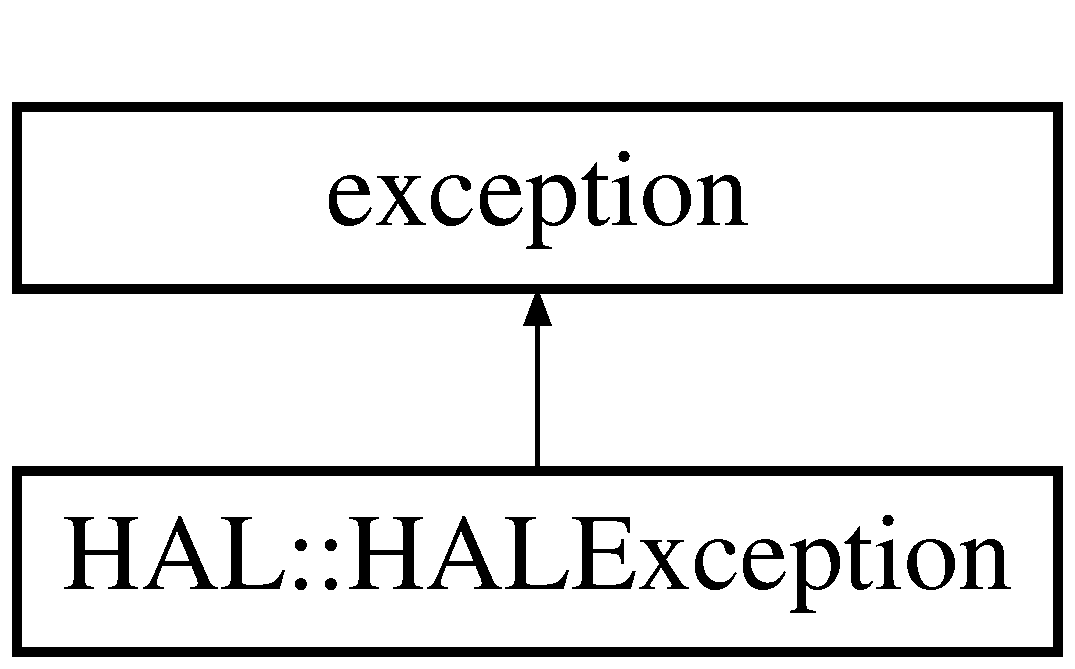
\includegraphics[height=2.000000cm]{class_h_a_l_1_1_h_a_l_exception}
\end{center}
\end{figure}
\subsection*{Public Member Functions}
\begin{DoxyCompactItemize}
\item 
\hypertarget{class_h_a_l_1_1_h_a_l_exception_a4f6662db7819d278a642abc8edf6b064}{{\bfseries H\+A\+L\+Exception} (T\+String m)}\label{class_h_a_l_1_1_h_a_l_exception_a4f6662db7819d278a642abc8edf6b064}

\item 
\hypertarget{class_h_a_l_1_1_h_a_l_exception_aaf6b8a29e7bb09721dd7aaa7b7a9b078}{virtual const char $\ast$ {\bfseries what} () const   throw ()}\label{class_h_a_l_1_1_h_a_l_exception_aaf6b8a29e7bb09721dd7aaa7b7a9b078}

\end{DoxyCompactItemize}


The documentation for this class was generated from the following file\+:\begin{DoxyCompactItemize}
\item 
/\+Users/jhetherly/src/\+H\+A\+L-\/\+R\+O\+O\+T/include/\+H\+A\+L/Exceptions.\+h\end{DoxyCompactItemize}

\hypertarget{class_h_a_l_1_1_algorithms_1_1_import_bool_value}{\section{H\+A\+L\+:\+:Algorithms\+:\+:Import\+Bool\+Value$<$ Value\+Getter $>$ Class Template Reference}
\label{class_h_a_l_1_1_algorithms_1_1_import_bool_value}\index{H\+A\+L\+::\+Algorithms\+::\+Import\+Bool\+Value$<$ Value\+Getter $>$@{H\+A\+L\+::\+Algorithms\+::\+Import\+Bool\+Value$<$ Value\+Getter $>$}}
}


\hyperlink{class_h_a_l_1_1_algorithm}{Algorithm} that stores a boolean value from information in a T\+Tree.  




{\ttfamily \#include $<$Import\+Value.\+h$>$}

Inheritance diagram for H\+A\+L\+:\+:Algorithms\+:\+:Import\+Bool\+Value$<$ Value\+Getter $>$\+:\begin{figure}[H]
\begin{center}
\leavevmode
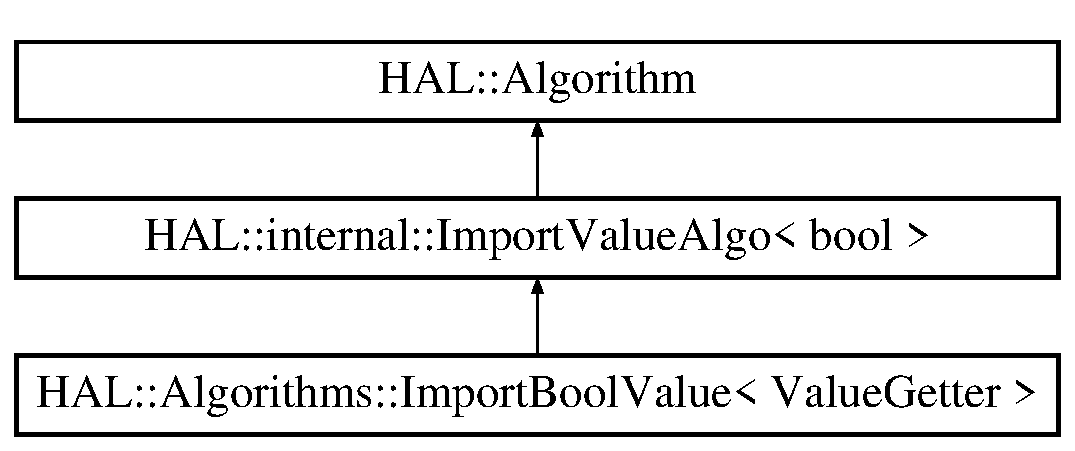
\includegraphics[height=3.000000cm]{class_h_a_l_1_1_algorithms_1_1_import_bool_value}
\end{center}
\end{figure}
\subsection*{Public Member Functions}
\begin{DoxyCompactItemize}
\item 
\hyperlink{class_h_a_l_1_1_algorithms_1_1_import_bool_value_a06b77726d1cfcd155fb7e28ee304a917}{Import\+Bool\+Value} (T\+String name, T\+String title)
\begin{DoxyCompactList}\small\item\em Constructor. \end{DoxyCompactList}\end{DoxyCompactItemize}
\subsection*{Protected Member Functions}
\begin{DoxyCompactItemize}
\item 
\hypertarget{class_h_a_l_1_1_algorithms_1_1_import_bool_value_a71a3ae1f800a947904fdf0d1c7af4c17}{virtual bool {\bfseries Get\+Value} ()}\label{class_h_a_l_1_1_algorithms_1_1_import_bool_value_a71a3ae1f800a947904fdf0d1c7af4c17}

\end{DoxyCompactItemize}
\subsection*{Protected Attributes}
\begin{DoxyCompactItemize}
\item 
\hypertarget{class_h_a_l_1_1_algorithms_1_1_import_bool_value_a8113934acb2bd48e34891d956f52c497}{Value\+Getter $\ast$ {\bfseries f\+Value\+Getter\+Ptr}}\label{class_h_a_l_1_1_algorithms_1_1_import_bool_value_a8113934acb2bd48e34891d956f52c497}

\end{DoxyCompactItemize}


\subsection{Detailed Description}
\subsubsection*{template$<$class Value\+Getter = H\+A\+L\+::\+Analysis\+Tree\+Reader$>$class H\+A\+L\+::\+Algorithms\+::\+Import\+Bool\+Value$<$ Value\+Getter $>$}

\hyperlink{class_h_a_l_1_1_algorithm}{Algorithm} that stores a boolean value from information in a T\+Tree. 

This algorithm imports the information to store a boolean value from a specified branch in a T\+Tree. The value from this algorithm is stored in a \hyperlink{class_h_a_l_1_1_generic_data}{Generic\+Data} object in the User\+Data under the algorithm's name and $<$name$>$\+:value.~\newline
~\newline
{\bfseries Explaination of the branch map\+:}~\newline
The required map is just one that points to the relavent boolean value. $<$name$>$ refers to the name given to this algorithm's constructor.~\newline
{\itshape Required Branch Map\+:} \begin{TabularC}{2}
\hline
\rowcolor{lightgray}{\bf }&\PBS\centering {\bf Boolean value  }\\\cline{1-2}
&\PBS\centering $<$name$>$\+:bool \\\cline{1-2}
\end{TabularC}
{\bfseries Note\+:} A custom value fetching class may be passed as a template arguement. This class must have constructor that accepts the T\+Tree as an arguement and overloads the () operator that accepts the entry number as an arguement. For example\+: 
\begin{DoxyCode}
\textcolor{preprocessor}{#include "TTreeReader.h"} \textcolor{comment}{// ROOT 6 tree reading class}
\textcolor{keyword}{class }MyTreeReader \{
\textcolor{keyword}{public}:
 \textcolor{comment}{// Needs a constructor like this}
 MyTreeReader (TTree *t) : tr(t), value(tr, \textcolor{stringliteral}{"my\_branch"}) \{\}
 \textcolor{comment}{// Needs operator() overloaded like this}
 \textcolor{keywordtype}{bool} operator (Long64\_t entry) \{
   tr.SetEntry(entry);
   \textcolor{keywordflow}{return} value;
 \}
\textcolor{keyword}{private}:
 TTreeReader tr;
 TTreeReaderValue<Bool\_t> value;
\};
\end{DoxyCode}
 {\bfseries Examples\+:}~\newline
In your analysis file, do the following to import a trigger flag\+:


\begin{DoxyCode}
\hyperlink{class_h_a_l_1_1_analysis}{HAL::Analysis} a(\textcolor{stringliteral}{"sample analysis"}, \textcolor{stringliteral}{""}, \textcolor{stringliteral}{"truth"});

a.AddAlgo(\textcolor{keyword}{new} \hyperlink{class_h_a_l_1_1_algorithms_1_1_import_bool_value}{HAL::Algorithms::ImportBool}(\textcolor{stringliteral}{"lepton trigger"}, \textcolor{stringliteral}{"import the lepton
       trigger"}));

\textcolor{comment}{//...}

a.MapBranch(\textcolor{stringliteral}{"some\_trigger\_branch"}, \textcolor{stringliteral}{"lepton trigger:bool"});
\end{DoxyCode}
 To import a value with a custom tree reading class, do the following\+:


\begin{DoxyCode}
\textcolor{preprocessor}{#include "MyTreeReader.h"}
\hyperlink{class_h_a_l_1_1_analysis}{HAL::Analysis} a(\textcolor{stringliteral}{"sample analysis"}, \textcolor{stringliteral}{""}, \textcolor{stringliteral}{"truth"});

a.AddAlgo(\textcolor{keyword}{new} \hyperlink{class_h_a_l_1_1_algorithms_1_1_import_bool_value}{HAL::Algorithms::ImportBoolValue<MyTreeReader>}(\textcolor{stringliteral}{
      "lepton trigger"}, 
                                                             \textcolor{stringliteral}{"import the lepton trigger"}));
\end{DoxyCode}
 

\subsection{Constructor \& Destructor Documentation}
\hypertarget{class_h_a_l_1_1_algorithms_1_1_import_bool_value_a06b77726d1cfcd155fb7e28ee304a917}{\index{H\+A\+L\+::\+Algorithms\+::\+Import\+Bool\+Value@{H\+A\+L\+::\+Algorithms\+::\+Import\+Bool\+Value}!Import\+Bool\+Value@{Import\+Bool\+Value}}
\index{Import\+Bool\+Value@{Import\+Bool\+Value}!H\+A\+L\+::\+Algorithms\+::\+Import\+Bool\+Value@{H\+A\+L\+::\+Algorithms\+::\+Import\+Bool\+Value}}
\subsubsection[{Import\+Bool\+Value}]{\setlength{\rightskip}{0pt plus 5cm}template$<$class Value\+Getter  = H\+A\+L\+::\+Analysis\+Tree\+Reader$>$ {\bf H\+A\+L\+::\+Algorithms\+::\+Import\+Bool\+Value}$<$ Value\+Getter $>$\+::{\bf Import\+Bool\+Value} (
\begin{DoxyParamCaption}
\item[{T\+String}]{name, }
\item[{T\+String}]{title}
\end{DoxyParamCaption}
)}}\label{class_h_a_l_1_1_algorithms_1_1_import_bool_value_a06b77726d1cfcd155fb7e28ee304a917}


Constructor. 

Initializes the algorithm 
\begin{DoxyParams}[1]{Parameters}
\mbox{\tt in}  & {\em name} & Name of the algorithm. This can be used as the input to other algorithms. \\
\hline
\mbox{\tt in}  & {\em title} & Description of the algorithm. Can be an empty string. \\
\hline
\end{DoxyParams}
\begin{DoxySeeAlso}{See also}
\hyperlink{class_h_a_l_1_1_algorithms_1_1_import_particle}{Import\+Particle}, Import\+Integer, Import\+Counting, Import\+Decimal 
\end{DoxySeeAlso}


The documentation for this class was generated from the following file\+:\begin{DoxyCompactItemize}
\item 
/\+Users/jhetherly/src/\+H\+A\+L-\/\+R\+O\+O\+T/include/\+H\+A\+L/\+Algorithms/\hyperlink{_import_value_8h}{Import\+Value.\+h}\end{DoxyCompactItemize}

\hypertarget{class_h_a_l_1_1_algorithms_1_1_import_counting_value}{\section{H\+A\+L\+:\+:Algorithms\+:\+:Import\+Counting\+Value$<$ Value\+Getter $>$ Class Template Reference}
\label{class_h_a_l_1_1_algorithms_1_1_import_counting_value}\index{H\+A\+L\+::\+Algorithms\+::\+Import\+Counting\+Value$<$ Value\+Getter $>$@{H\+A\+L\+::\+Algorithms\+::\+Import\+Counting\+Value$<$ Value\+Getter $>$}}
}


\hyperlink{class_h_a_l_1_1_algorithm}{Algorithm} that stores a counting value from information in a T\+Tree.  




{\ttfamily \#include $<$Import\+Value.\+h$>$}

Inheritance diagram for H\+A\+L\+:\+:Algorithms\+:\+:Import\+Counting\+Value$<$ Value\+Getter $>$\+:\begin{figure}[H]
\begin{center}
\leavevmode
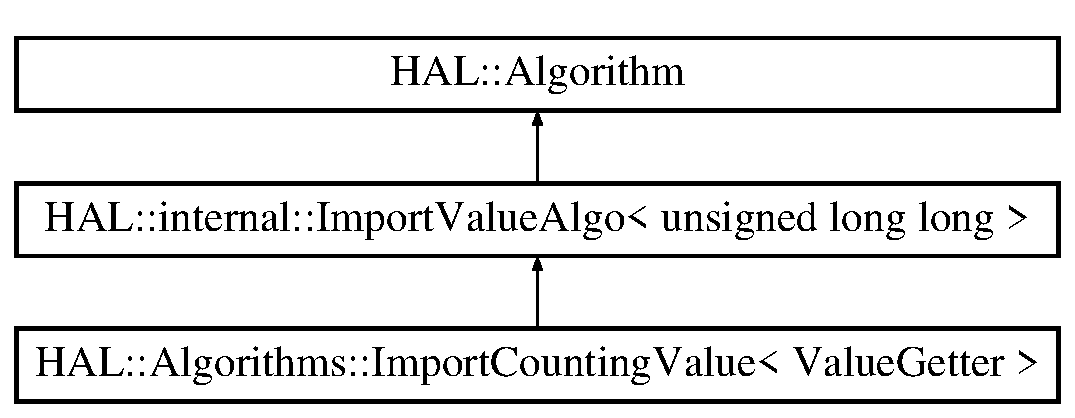
\includegraphics[height=3.000000cm]{class_h_a_l_1_1_algorithms_1_1_import_counting_value}
\end{center}
\end{figure}
\subsection*{Public Member Functions}
\begin{DoxyCompactItemize}
\item 
\hyperlink{class_h_a_l_1_1_algorithms_1_1_import_counting_value_a9abeea49a97ffe789dc1e70a2436b027}{Import\+Counting\+Value} (T\+String name, T\+String title)
\begin{DoxyCompactList}\small\item\em Constructor. \end{DoxyCompactList}\end{DoxyCompactItemize}
\subsection*{Protected Member Functions}
\begin{DoxyCompactItemize}
\item 
\hypertarget{class_h_a_l_1_1_algorithms_1_1_import_counting_value_ae56b3039650722c791d2635039937f59}{virtual unsigned long long {\bfseries Get\+Value} ()}\label{class_h_a_l_1_1_algorithms_1_1_import_counting_value_ae56b3039650722c791d2635039937f59}

\item 
\hypertarget{class_h_a_l_1_1_algorithms_1_1_import_counting_value_a55d90364aba22128a661036ee6554b08}{{\footnotesize template$<$$>$ }\\unsigned long long {\bfseries Get\+Value} ()}\label{class_h_a_l_1_1_algorithms_1_1_import_counting_value_a55d90364aba22128a661036ee6554b08}

\end{DoxyCompactItemize}
\subsection*{Protected Attributes}
\begin{DoxyCompactItemize}
\item 
\hypertarget{class_h_a_l_1_1_algorithms_1_1_import_counting_value_ab93d369be3c197cadce57e1d5eb8a47e}{Value\+Getter $\ast$ {\bfseries f\+Value\+Getter\+Ptr}}\label{class_h_a_l_1_1_algorithms_1_1_import_counting_value_ab93d369be3c197cadce57e1d5eb8a47e}

\end{DoxyCompactItemize}


\subsection{Detailed Description}
\subsubsection*{template$<$class Value\+Getter = H\+A\+L\+::\+Analysis\+Tree\+Reader$>$class H\+A\+L\+::\+Algorithms\+::\+Import\+Counting\+Value$<$ Value\+Getter $>$}

\hyperlink{class_h_a_l_1_1_algorithm}{Algorithm} that stores a counting value from information in a T\+Tree. 

This algorithm imports the information to store a counting value from a specified branch in a T\+Tree. The value from this algorithm is stored in a \hyperlink{class_h_a_l_1_1_generic_data}{Generic\+Data} object in the User\+Data under the algorithm's name and $<$name$>$\+:value.~\newline
~\newline
{\bfseries Explaination of the branch map\+:}~\newline
The required map is just one that points to the relavent counting value. $<$name$>$ refers to the name given to this algorithm's constructor.~\newline
{\itshape Required Branch Map\+:} \begin{TabularC}{2}
\hline
\rowcolor{lightgray}{\bf }&\PBS\centering {\bf Counting value  }\\\cline{1-2}
&\PBS\centering $<$name$>$\+:counting \\\cline{1-2}
\end{TabularC}
{\bfseries Note\+:} A custom value fetching class may be passed as a template arguement. This class must have constructor that accepts the T\+Tree as an arguement and overloads the () operator that accepts the entry number as an arguement. For example\+: 
\begin{DoxyCode}
\textcolor{preprocessor}{#include "TTreeReader.h"} \textcolor{comment}{// ROOT 6 tree reading class}
\textcolor{preprocessor}{#include "TTreeReaderValue.h"}

\textcolor{keyword}{class }MyTreeReader \{
\textcolor{keyword}{public}:
 \textcolor{comment}{// Needs a constructor like this}
 MyTreeReader (TTree *t) : tr(t), value(tr, \textcolor{stringliteral}{"my\_branch"}) \{\}
 \textcolor{comment}{// Needs operator() overloaded like this}
 \textcolor{keywordtype}{unsigned} \textcolor{keywordtype}{long} \textcolor{keywordtype}{long} operator (Long64\_t entry) \{
   tr.SetEntry(entry);
   \textcolor{keywordflow}{return} *value;
 \}
\textcolor{keyword}{private}:
 TTreeReader tr;
 TTreeReaderValue<UInt\_t> value;
\};
\end{DoxyCode}
 {\bfseries Example\+:}~\newline
In your analysis file, do the following for a counting value\+:


\begin{DoxyCode}
\hyperlink{class_h_a_l_1_1_analysis}{HAL::Analysis} a(\textcolor{stringliteral}{"sample analysis"}, \textcolor{stringliteral}{""}, \textcolor{stringliteral}{"truth"});

a.AddAlgo(\textcolor{keyword}{new} HAL::Algorithms::ImportCounting(\textcolor{stringliteral}{"counting value"}, \textcolor{stringliteral}{"import a counting value"}));

\textcolor{comment}{//...}

a.MapBranch(\textcolor{stringliteral}{"some\_counting\_branch"}, \textcolor{stringliteral}{"counting value:counting"});
\end{DoxyCode}
 To import a value with a custom tree reading class, do the following\+:


\begin{DoxyCode}
\textcolor{preprocessor}{#include "MyTreeReader.h"}
\hyperlink{class_h_a_l_1_1_analysis}{HAL::Analysis} a(\textcolor{stringliteral}{"sample analysis"}, \textcolor{stringliteral}{""}, \textcolor{stringliteral}{"truth"});

a.AddAlgo(\textcolor{keyword}{new} \hyperlink{class_h_a_l_1_1_algorithms_1_1_import_counting_value}{HAL::Algorithms::ImportCountingValue<MyTreeReader>}
      (\textcolor{stringliteral}{"counting value"}, 
                                                                 \textcolor{stringliteral}{"import an counting value"}));
\end{DoxyCode}
 

\subsection{Constructor \& Destructor Documentation}
\hypertarget{class_h_a_l_1_1_algorithms_1_1_import_counting_value_a9abeea49a97ffe789dc1e70a2436b027}{\index{H\+A\+L\+::\+Algorithms\+::\+Import\+Counting\+Value@{H\+A\+L\+::\+Algorithms\+::\+Import\+Counting\+Value}!Import\+Counting\+Value@{Import\+Counting\+Value}}
\index{Import\+Counting\+Value@{Import\+Counting\+Value}!H\+A\+L\+::\+Algorithms\+::\+Import\+Counting\+Value@{H\+A\+L\+::\+Algorithms\+::\+Import\+Counting\+Value}}
\subsubsection[{Import\+Counting\+Value}]{\setlength{\rightskip}{0pt plus 5cm}template$<$class Value\+Getter $>$ {\bf H\+A\+L\+::\+Algorithms\+::\+Import\+Counting\+Value}$<$ Value\+Getter $>$\+::{\bf Import\+Counting\+Value} (
\begin{DoxyParamCaption}
\item[{T\+String}]{name, }
\item[{T\+String}]{title}
\end{DoxyParamCaption}
)}}\label{class_h_a_l_1_1_algorithms_1_1_import_counting_value_a9abeea49a97ffe789dc1e70a2436b027}


Constructor. 

Initializes the algorithm 
\begin{DoxyParams}[1]{Parameters}
\mbox{\tt in}  & {\em name} & Name of the algorithm. This can be used as the input to other algorithms. \\
\hline
\mbox{\tt in}  & {\em title} & Description of the algorithm. Can be an empty string. \\
\hline
\end{DoxyParams}
\begin{DoxySeeAlso}{See also}
Import\+Bool, Import\+Integer, \hyperlink{class_h_a_l_1_1_algorithms_1_1_import_particle}{Import\+Particle}, Import\+Decimal 
\end{DoxySeeAlso}


The documentation for this class was generated from the following file\+:\begin{DoxyCompactItemize}
\item 
/\+Users/jhetherly/src/\+H\+A\+L-\/\+R\+O\+O\+T/include/\+H\+A\+L/\+Algorithms/\hyperlink{_import_value_8h}{Import\+Value.\+h}\end{DoxyCompactItemize}

\hypertarget{class_h_a_l_1_1_algorithms_1_1_import_decimal_value}{\section{H\+A\+L\+:\+:Algorithms\+:\+:Import\+Decimal\+Value$<$ Value\+Getter $>$ Class Template Reference}
\label{class_h_a_l_1_1_algorithms_1_1_import_decimal_value}\index{H\+A\+L\+::\+Algorithms\+::\+Import\+Decimal\+Value$<$ Value\+Getter $>$@{H\+A\+L\+::\+Algorithms\+::\+Import\+Decimal\+Value$<$ Value\+Getter $>$}}
}


\hyperlink{class_h_a_l_1_1_algorithm}{Algorithm} that stores a decimal value from information in a T\+Tree.  




{\ttfamily \#include $<$Import\+Value.\+h$>$}

Inheritance diagram for H\+A\+L\+:\+:Algorithms\+:\+:Import\+Decimal\+Value$<$ Value\+Getter $>$\+:\begin{figure}[H]
\begin{center}
\leavevmode
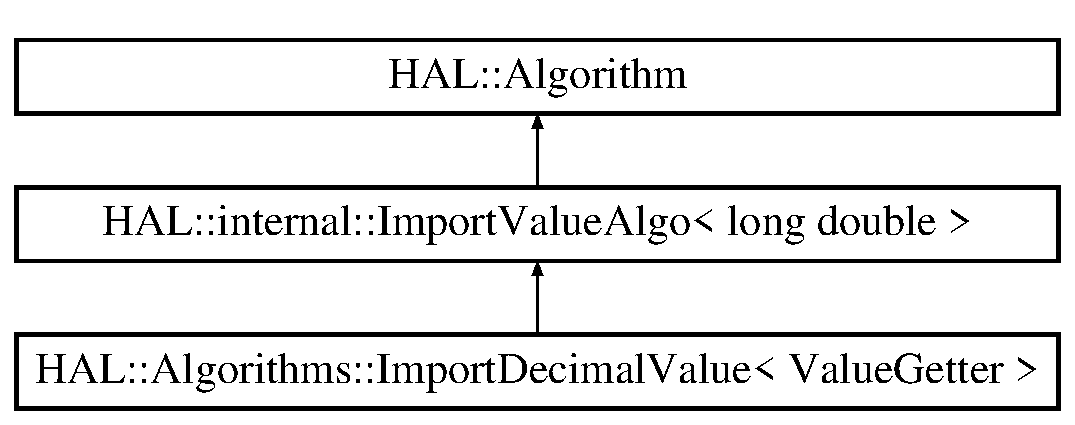
\includegraphics[height=3.000000cm]{class_h_a_l_1_1_algorithms_1_1_import_decimal_value}
\end{center}
\end{figure}
\subsection*{Public Member Functions}
\begin{DoxyCompactItemize}
\item 
\hyperlink{class_h_a_l_1_1_algorithms_1_1_import_decimal_value_aa1f2c9f13b324cbef3d8632b64e21419}{Import\+Decimal\+Value} (T\+String name, T\+String title)
\begin{DoxyCompactList}\small\item\em Constructor. \end{DoxyCompactList}\end{DoxyCompactItemize}
\subsection*{Protected Member Functions}
\begin{DoxyCompactItemize}
\item 
\hypertarget{class_h_a_l_1_1_algorithms_1_1_import_decimal_value_aaa975cb712b925aae8dd1a4ed7acfa41}{virtual long double {\bfseries Get\+Value} ()}\label{class_h_a_l_1_1_algorithms_1_1_import_decimal_value_aaa975cb712b925aae8dd1a4ed7acfa41}

\end{DoxyCompactItemize}
\subsection*{Protected Attributes}
\begin{DoxyCompactItemize}
\item 
\hypertarget{class_h_a_l_1_1_algorithms_1_1_import_decimal_value_abd097dd9e4459fe8c726305e602f1def}{Value\+Getter $\ast$ {\bfseries f\+Value\+Getter\+Ptr}}\label{class_h_a_l_1_1_algorithms_1_1_import_decimal_value_abd097dd9e4459fe8c726305e602f1def}

\end{DoxyCompactItemize}


\subsection{Detailed Description}
\subsubsection*{template$<$class Value\+Getter = H\+A\+L\+::\+Analysis\+Tree\+Reader$>$class H\+A\+L\+::\+Algorithms\+::\+Import\+Decimal\+Value$<$ Value\+Getter $>$}

\hyperlink{class_h_a_l_1_1_algorithm}{Algorithm} that stores a decimal value from information in a T\+Tree. 

This algorithm imports the information to store a decimal value from a specified branch in a T\+Tree. The value from this algorithm is stored in a \hyperlink{class_h_a_l_1_1_generic_data}{Generic\+Data} object in the User\+Data under the algorithm's name and $<$name$>$\+:value.~\newline
~\newline
{\bfseries Explaination of the branch map\+:}~\newline
The required map is just one that points to the relavent decimal value. $<$name$>$ refers to the name given to this algorithm's constructor.~\newline
{\itshape Required Branch Map\+:} \begin{TabularC}{2}
\hline
\rowcolor{lightgray}{\bf }&\PBS\centering {\bf Decimal value  }\\\cline{1-2}
&\PBS\centering $<$name$>$\+:decimal \\\cline{1-2}
\end{TabularC}
{\bfseries Note\+:} A custom value fetching class may be passed as a template arguement. This class must have constructor that accepts the T\+Tree as an arguement and overloads the () operator that accepts the entry number as an arguement. For example\+: 
\begin{DoxyCode}
\textcolor{preprocessor}{#include "TTreeReader.h"} \textcolor{comment}{// ROOT 6 tree reading class}
\textcolor{keyword}{class }MyTreeReader \{
\textcolor{keyword}{public}:
 \textcolor{comment}{// Needs a constructor like this}
 MyTreeReader (TTree *t) : tr(t), value(tr, \textcolor{stringliteral}{"my\_branch"}) \{\}
 \textcolor{comment}{// Needs operator() overloaded like this}
 \textcolor{keywordtype}{long} \textcolor{keywordtype}{double} operator (Long64\_t entry) \{
   tr.SetEntry(entry);
   \textcolor{keywordflow}{return} value;
 \}
\textcolor{keyword}{private}:
 TTreeReader tr;
 TTreeReaderValue<Float\_t> value;
\};
\end{DoxyCode}
 {\bfseries Example\+:}~\newline
In your analysis file, do the following for a decimal value\+:


\begin{DoxyCode}
\hyperlink{class_h_a_l_1_1_analysis}{HAL::Analysis} a(\textcolor{stringliteral}{"sample analysis"}, \textcolor{stringliteral}{""}, \textcolor{stringliteral}{"truth"});

a.AddAlgo(\textcolor{keyword}{new} \hyperlink{class_h_a_l_1_1_algorithms_1_1_import_decimal_value}{HAL::Algorithms::ImportDecimal}(\textcolor{stringliteral}{"decimal value"}, \textcolor{stringliteral}{"import a
       decimal value"}));

\textcolor{comment}{//...}

a.MapBranch(\textcolor{stringliteral}{"some\_decimal\_branch"}, \textcolor{stringliteral}{"decimal value:decimal"});
\end{DoxyCode}
 To import a value with a custom tree reading class, do the following\+:


\begin{DoxyCode}
\textcolor{preprocessor}{#include "MyTreeReader.h"}
\hyperlink{class_h_a_l_1_1_analysis}{HAL::Analysis} a(\textcolor{stringliteral}{"sample analysis"}, \textcolor{stringliteral}{""}, \textcolor{stringliteral}{"truth"});

a.AddAlgo(\textcolor{keyword}{new} \hyperlink{class_h_a_l_1_1_algorithms_1_1_import_decimal_value}{HAL::Algorithms::ImportDecimalValue<MyTreeReader>}
      (\textcolor{stringliteral}{"decimal value"}, 
                                                                \textcolor{stringliteral}{"import an decimal value"}));
\end{DoxyCode}
 

\subsection{Constructor \& Destructor Documentation}
\hypertarget{class_h_a_l_1_1_algorithms_1_1_import_decimal_value_aa1f2c9f13b324cbef3d8632b64e21419}{\index{H\+A\+L\+::\+Algorithms\+::\+Import\+Decimal\+Value@{H\+A\+L\+::\+Algorithms\+::\+Import\+Decimal\+Value}!Import\+Decimal\+Value@{Import\+Decimal\+Value}}
\index{Import\+Decimal\+Value@{Import\+Decimal\+Value}!H\+A\+L\+::\+Algorithms\+::\+Import\+Decimal\+Value@{H\+A\+L\+::\+Algorithms\+::\+Import\+Decimal\+Value}}
\subsubsection[{Import\+Decimal\+Value}]{\setlength{\rightskip}{0pt plus 5cm}template$<$class Value\+Getter  = H\+A\+L\+::\+Analysis\+Tree\+Reader$>$ {\bf H\+A\+L\+::\+Algorithms\+::\+Import\+Decimal\+Value}$<$ Value\+Getter $>$\+::{\bf Import\+Decimal\+Value} (
\begin{DoxyParamCaption}
\item[{T\+String}]{name, }
\item[{T\+String}]{title}
\end{DoxyParamCaption}
)}}\label{class_h_a_l_1_1_algorithms_1_1_import_decimal_value_aa1f2c9f13b324cbef3d8632b64e21419}


Constructor. 

Initializes the algorithm 
\begin{DoxyParams}[1]{Parameters}
\mbox{\tt in}  & {\em name} & Name of the algorithm. This can be used as the input to other algorithms. \\
\hline
\mbox{\tt in}  & {\em title} & Description of the algorithm. Can be an empty string. \\
\hline
\end{DoxyParams}
\begin{DoxySeeAlso}{See also}
Import\+Bool, Import\+Integer, Import\+Counting, \hyperlink{class_h_a_l_1_1_algorithms_1_1_import_particle}{Import\+Particle} 
\end{DoxySeeAlso}


The documentation for this class was generated from the following file\+:\begin{DoxyCompactItemize}
\item 
/\+Users/jhetherly/src/\+H\+A\+L-\/\+R\+O\+O\+T/include/\+H\+A\+L/\+Algorithms/\hyperlink{_import_value_8h}{Import\+Value.\+h}\end{DoxyCompactItemize}

\hypertarget{class_h_a_l_1_1_algorithms_1_1_import_integer_value}{\section{H\+A\+L\+:\+:Algorithms\+:\+:Import\+Integer\+Value$<$ Value\+Getter $>$ Class Template Reference}
\label{class_h_a_l_1_1_algorithms_1_1_import_integer_value}\index{H\+A\+L\+::\+Algorithms\+::\+Import\+Integer\+Value$<$ Value\+Getter $>$@{H\+A\+L\+::\+Algorithms\+::\+Import\+Integer\+Value$<$ Value\+Getter $>$}}
}


\hyperlink{class_h_a_l_1_1_algorithm}{Algorithm} that stores an integer value from information in a T\+Tree.  




{\ttfamily \#include $<$Import\+Value.\+h$>$}

Inheritance diagram for H\+A\+L\+:\+:Algorithms\+:\+:Import\+Integer\+Value$<$ Value\+Getter $>$\+:\begin{figure}[H]
\begin{center}
\leavevmode
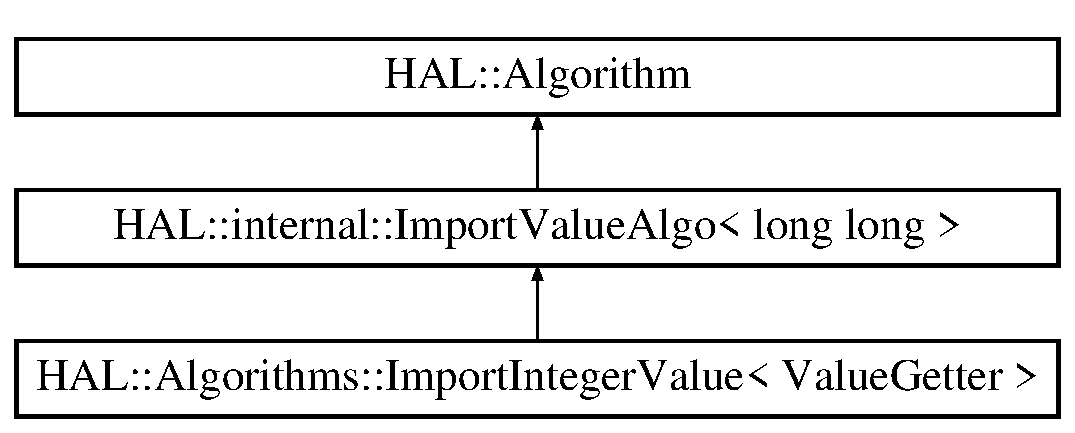
\includegraphics[height=3.000000cm]{class_h_a_l_1_1_algorithms_1_1_import_integer_value}
\end{center}
\end{figure}
\subsection*{Public Member Functions}
\begin{DoxyCompactItemize}
\item 
\hyperlink{class_h_a_l_1_1_algorithms_1_1_import_integer_value_a19a3f6712ad9a986d98c6da3a9b196ec}{Import\+Integer\+Value} (T\+String name, T\+String title)
\begin{DoxyCompactList}\small\item\em Constructor. \end{DoxyCompactList}\end{DoxyCompactItemize}
\subsection*{Protected Member Functions}
\begin{DoxyCompactItemize}
\item 
\hypertarget{class_h_a_l_1_1_algorithms_1_1_import_integer_value_a48b6c6c4e7471ce8aa79f1ed20f7d306}{virtual long long {\bfseries Get\+Value} ()}\label{class_h_a_l_1_1_algorithms_1_1_import_integer_value_a48b6c6c4e7471ce8aa79f1ed20f7d306}

\end{DoxyCompactItemize}
\subsection*{Protected Attributes}
\begin{DoxyCompactItemize}
\item 
\hypertarget{class_h_a_l_1_1_algorithms_1_1_import_integer_value_af6ad5771bb63a3e813583f428095e831}{Value\+Getter $\ast$ {\bfseries f\+Value\+Getter\+Ptr}}\label{class_h_a_l_1_1_algorithms_1_1_import_integer_value_af6ad5771bb63a3e813583f428095e831}

\end{DoxyCompactItemize}


\subsection{Detailed Description}
\subsubsection*{template$<$class Value\+Getter = H\+A\+L\+::\+Analysis\+Tree\+Reader$>$class H\+A\+L\+::\+Algorithms\+::\+Import\+Integer\+Value$<$ Value\+Getter $>$}

\hyperlink{class_h_a_l_1_1_algorithm}{Algorithm} that stores an integer value from information in a T\+Tree. 

This algorithm imports the information to store an integer value from a specified branch in a T\+Tree. The value from this algorithm is stored in a \hyperlink{class_h_a_l_1_1_generic_data}{Generic\+Data} object in the User\+Data under the algorithm's name and $<$name$>$\+:value.~\newline
~\newline
{\bfseries Explaination of the branch map\+:}~\newline
The required map is just one that points to the relavent integer value. $<$name$>$ refers to the name given to this algorithm's constructor.~\newline
{\itshape Required Branch Map\+:} \begin{TabularC}{2}
\hline
\rowcolor{lightgray}{\bf }&\PBS\centering {\bf Integer value  }\\\cline{1-2}
&\PBS\centering $<$name$>$\+:integer \\\cline{1-2}
\end{TabularC}
{\bfseries Note\+:} A custom value fetching class may be passed as a template arguement. This class must have constructor that accepts the T\+Tree as an arguement and overloads the () operator that accepts the entry number as an arguement. For example\+: 
\begin{DoxyCode}
\textcolor{preprocessor}{#include "TTreeReader.h"} \textcolor{comment}{// ROOT 6 tree reading class}
\textcolor{keyword}{class }MyTreeReader \{
\textcolor{keyword}{public}:
 \textcolor{comment}{// Needs a constructor like this}
 MyTreeReader (TTree *t) : tr(t), value(tr, \textcolor{stringliteral}{"my\_branch"}) \{\}
 \textcolor{comment}{// Needs operator() overloaded like this}
 \textcolor{keywordtype}{long} \textcolor{keywordtype}{long} operator (Long64\_t entry) \{
   tr.SetEntry(entry);
   \textcolor{keywordflow}{return} value;
 \}
\textcolor{keyword}{private}:
 TTreeReader tr;
 TTreeReaderValue<Int\_t> value;
\};
\end{DoxyCode}
 {\bfseries Example\+:}~\newline
In your analysis file, do the following for an integer value\+:


\begin{DoxyCode}
\hyperlink{class_h_a_l_1_1_analysis}{HAL::Analysis} a(\textcolor{stringliteral}{"sample analysis"}, \textcolor{stringliteral}{""}, \textcolor{stringliteral}{"truth"});

a.AddAlgo(\textcolor{keyword}{new} \hyperlink{class_h_a_l_1_1_algorithms_1_1_import_integer_value}{HAL::Algorithms::ImportInteger}(\textcolor{stringliteral}{"integer value"}, \textcolor{stringliteral}{"import an
       integer value"}));

\textcolor{comment}{//...}

a.MapBranch(\textcolor{stringliteral}{"some\_integer\_branch"}, \textcolor{stringliteral}{"integer value:integer"});
\end{DoxyCode}
 To import a value with a custom tree reading class, do the following\+:


\begin{DoxyCode}
\textcolor{preprocessor}{#include "MyTreeReader.h"}
\hyperlink{class_h_a_l_1_1_analysis}{HAL::Analysis} a(\textcolor{stringliteral}{"sample analysis"}, \textcolor{stringliteral}{""}, \textcolor{stringliteral}{"truth"});

a.AddAlgo(\textcolor{keyword}{new} \hyperlink{class_h_a_l_1_1_algorithms_1_1_import_integer_value}{HAL::Algorithms::ImportIntegerValue<MyTreeReader>}
      (\textcolor{stringliteral}{"integer value"}, 
                                                                \textcolor{stringliteral}{"import an integer value"}));
\end{DoxyCode}
 

\subsection{Constructor \& Destructor Documentation}
\hypertarget{class_h_a_l_1_1_algorithms_1_1_import_integer_value_a19a3f6712ad9a986d98c6da3a9b196ec}{\index{H\+A\+L\+::\+Algorithms\+::\+Import\+Integer\+Value@{H\+A\+L\+::\+Algorithms\+::\+Import\+Integer\+Value}!Import\+Integer\+Value@{Import\+Integer\+Value}}
\index{Import\+Integer\+Value@{Import\+Integer\+Value}!H\+A\+L\+::\+Algorithms\+::\+Import\+Integer\+Value@{H\+A\+L\+::\+Algorithms\+::\+Import\+Integer\+Value}}
\subsubsection[{Import\+Integer\+Value}]{\setlength{\rightskip}{0pt plus 5cm}template$<$class Value\+Getter  = H\+A\+L\+::\+Analysis\+Tree\+Reader$>$ {\bf H\+A\+L\+::\+Algorithms\+::\+Import\+Integer\+Value}$<$ Value\+Getter $>$\+::{\bf Import\+Integer\+Value} (
\begin{DoxyParamCaption}
\item[{T\+String}]{name, }
\item[{T\+String}]{title}
\end{DoxyParamCaption}
)}}\label{class_h_a_l_1_1_algorithms_1_1_import_integer_value_a19a3f6712ad9a986d98c6da3a9b196ec}


Constructor. 

Initializes the algorithm 
\begin{DoxyParams}[1]{Parameters}
\mbox{\tt in}  & {\em name} & Name of the algorithm. This can be used as the input to other algorithms. \\
\hline
\mbox{\tt in}  & {\em title} & Description of the algorithm. Can be an empty string. \\
\hline
\end{DoxyParams}
\begin{DoxySeeAlso}{See also}
Import\+Bool, \hyperlink{class_h_a_l_1_1_algorithms_1_1_import_particle}{Import\+Particle}, Import\+Counting, Import\+Decimal 
\end{DoxySeeAlso}


The documentation for this class was generated from the following file\+:\begin{DoxyCompactItemize}
\item 
/\+Users/jhetherly/src/\+H\+A\+L-\/\+R\+O\+O\+T/include/\+H\+A\+L/\+Algorithms/\hyperlink{_import_value_8h}{Import\+Value.\+h}\end{DoxyCompactItemize}

\hypertarget{class_h_a_l_1_1_algorithms_1_1_import_particle}{\section{H\-A\-L\-:\-:Algorithms\-:\-:Import\-Particle Class Reference}
\label{class_h_a_l_1_1_algorithms_1_1_import_particle}\index{H\-A\-L\-::\-Algorithms\-::\-Import\-Particle@{H\-A\-L\-::\-Algorithms\-::\-Import\-Particle}}
}


Generic algorithm class that builds particles from information in a T\-Tree.  




{\ttfamily \#include $<$Algorithms.\-h$>$}

Inheritance diagram for H\-A\-L\-:\-:Algorithms\-:\-:Import\-Particle\-:\begin{figure}[H]
\begin{center}
\leavevmode
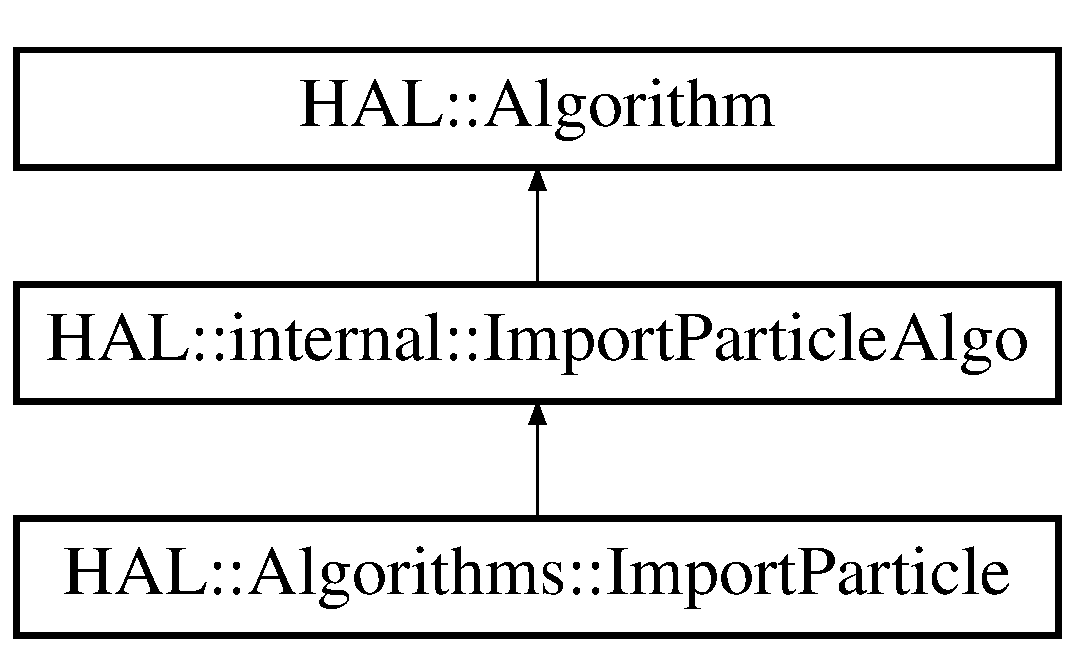
\includegraphics[height=3.000000cm]{class_h_a_l_1_1_algorithms_1_1_import_particle}
\end{center}
\end{figure}
\subsection*{Public Member Functions}
\begin{DoxyCompactItemize}
\item 
\hyperlink{class_h_a_l_1_1_algorithms_1_1_import_particle_ab42dcac49ed8ae1f565346ec7372c7a5}{Import\-Particle} (T\-String name, T\-String title, unsigned n\-\_\-max=0)
\begin{DoxyCompactList}\small\item\em Constructor. \end{DoxyCompactList}\end{DoxyCompactItemize}
\subsection*{Protected Member Functions}
\begin{DoxyCompactItemize}
\item 
\hypertarget{class_h_a_l_1_1_algorithms_1_1_import_particle_a1e5924b9deb6c7d1c1d1734b8cb510cb}{virtual void {\bfseries Exec} (Option\-\_\-t $\ast$)}\label{class_h_a_l_1_1_algorithms_1_1_import_particle_a1e5924b9deb6c7d1c1d1734b8cb510cb}

\item 
\hypertarget{class_h_a_l_1_1_algorithms_1_1_import_particle_abad1a5a9b44becfae4e4a7113edc80eb}{virtual T\-Lorentz\-Vector $\ast$ {\bfseries Make\-T\-L\-V} (unsigned)}\label{class_h_a_l_1_1_algorithms_1_1_import_particle_abad1a5a9b44becfae4e4a7113edc80eb}

\end{DoxyCompactItemize}
\subsection*{Additional Inherited Members}


\subsection{Detailed Description}
Generic algorithm class that builds particles from information in a T\-Tree. 

This algorithm imports the information to build particles from specified branches in a T\-Tree. It may use the branches to build particles with either full 4-\/vector momentum or transverse momentum. It can optionally read in the charge, particle I\-D, and number of particles to import. It determines how to read in the particles through the specified branch maps given to the \hyperlink{class_h_a_l_1_1_analysis}{Analysis} object. It can also determine how many particles to read in based on whether you give a number to read, branchmap to scan, or implicitly gather it from the length of the other required branches. The necessary branch maps are given below. The particles from this algorithm are stored in a \hyperlink{class_h_a_l_1_1_generic_data}{Generic\-Data} object in the User\-Data under the algorithm's name.\par
\par
 {\bfseries Explaination of the branch maps\-:}\par
 The required maps are those needed to construct the T\-Lorentz\-Vectors, either complete vectors or just transverse vectors. Any set of the branch maps given below will do. $<$name$>$ refers to the name given to this algorithm's constructor.\par
 {\itshape Required Branch Maps\-:} \begin{TabularC}{6}
\hline
\rowcolor{lightgray}\PBS\centering {\bf Cartesian components }&\PBS\centering {\bf $ p_T,\eta,\phi,E$ }&\PBS\centering {\bf $ p_T,\eta,\phi,m$ }&\PBS\centering {\bf Transverse Cartesian }&\PBS\centering {\bf $ p_T,\phi$ }&\PBS\centering {\bf $ E_T,\phi$ }\\\cline{1-6}
\PBS\centering $<$name$>$\-:x0 &\PBS\centering $<$name$>$\-:pt &\PBS\centering $<$name$>$\-:pt &\PBS\centering $<$name$>$\-:x1 &\PBS\centering $<$name$>$\-:pt &\PBS\centering $<$name$>$\-:et \\\cline{1-6}
\PBS\centering $<$name$>$\-:x1 &\PBS\centering $<$name$>$\-:eta &\PBS\centering $<$name$>$\-:eta &\PBS\centering $<$name$>$\-:x2 &\PBS\centering $<$name$>$\-:phi &\PBS\centering $<$name$>$\-:phi \\\cline{1-6}
\PBS\centering $<$name$>$\-:x2 &\PBS\centering $<$name$>$\-:phi &\PBS\centering $<$name$>$\-:phi &\PBS\centering &\PBS\centering &\PBS\centering \\\cline{1-6}
\PBS\centering $<$name$>$\-:x3 &\PBS\centering $<$name$>$\-:e &\PBS\centering $<$name$>$\-:m &\PBS\centering &\PBS\centering &\PBS\centering \\\cline{1-6}
\end{TabularC}
{\itshape Optional Branch Maps\-:} \begin{TabularC}{3}
\hline
\rowcolor{lightgray}\PBS\centering {\bf Number of particle }&\PBS\centering {\bf Charge }&\PBS\centering {\bf I\-D }\\\cline{1-3}
\PBS\centering $<$name$>$\-:nentries &\PBS\centering $<$name$>$\-:charge &\PBS\centering $<$name$>$\-:id \\\cline{1-3}
\end{TabularC}
{\bfseries Examples\-:}\par
 In your analysis file, do the following to import Monte Carlo particles with complete 4-\/vectors\-:


\begin{DoxyCode}
\hyperlink{class_h_a_l_1_1_analysis}{HAL::Analysis} a(\textcolor{stringliteral}{"sample analysis"}, \textcolor{stringliteral}{""}, \textcolor{stringliteral}{"truth"});

a.AddAlgo(\textcolor{keyword}{new} \hyperlink{class_h_a_l_1_1_algorithms_1_1_import_particle}{HAL::Algorithms::ImportParticle}(\textcolor{stringliteral}{"mc"}, \textcolor{stringliteral}{"import basic Monte
       Carlo particles"}));

\textcolor{comment}{//...}

a.MapBranch(\textcolor{stringliteral}{"mc\_pt"},     \textcolor{stringliteral}{"mc:pt"});
a.MapBranch(\textcolor{stringliteral}{"mc\_eta"},    \textcolor{stringliteral}{"mc:eta"});
a.MapBranch(\textcolor{stringliteral}{"mc\_phi"},    \textcolor{stringliteral}{"mc:phi"});
a.MapBranch(\textcolor{stringliteral}{"mc\_m"},      \textcolor{stringliteral}{"mc:m"});
a.MapBranch(\textcolor{stringliteral}{"mc\_pdgId"},  \textcolor{stringliteral}{"mc:id"});
a.MapBranch(\textcolor{stringliteral}{"mc\_charge"}, \textcolor{stringliteral}{"mc:charge"});
\end{DoxyCode}
 Likewise, you can import the M\-E\-T vector like so\-:


\begin{DoxyCode}
\hyperlink{class_h_a_l_1_1_analysis}{HAL::Analysis} a(\textcolor{stringliteral}{"sample analysis"}, \textcolor{stringliteral}{""}, \textcolor{stringliteral}{"truth"});

a.AddAlgo(\textcolor{keyword}{new} \hyperlink{class_h_a_l_1_1_algorithms_1_1_import_particle}{HAL::Algorithms::ImportParticle}(\textcolor{stringliteral}{"met"}, \textcolor{stringliteral}{"import the MET
       tranverse vector"}));

\textcolor{comment}{//...}

a.MapBranch(\textcolor{stringliteral}{"MET\_Truth\_Int\_etx"}, \textcolor{stringliteral}{"met:x1"});
a.MapBranch(\textcolor{stringliteral}{"MET\_Truth\_Int\_ety"}, \textcolor{stringliteral}{"met:x2"});
\end{DoxyCode}
 

\subsection{Constructor \& Destructor Documentation}
\hypertarget{class_h_a_l_1_1_algorithms_1_1_import_particle_ab42dcac49ed8ae1f565346ec7372c7a5}{\index{H\-A\-L\-::\-Algorithms\-::\-Import\-Particle@{H\-A\-L\-::\-Algorithms\-::\-Import\-Particle}!Import\-Particle@{Import\-Particle}}
\index{Import\-Particle@{Import\-Particle}!HAL::Algorithms::ImportParticle@{H\-A\-L\-::\-Algorithms\-::\-Import\-Particle}}
\subsubsection[{Import\-Particle}]{\setlength{\rightskip}{0pt plus 5cm}H\-A\-L\-::\-Algorithms\-::\-Import\-Particle\-::\-Import\-Particle (
\begin{DoxyParamCaption}
\item[{T\-String}]{name, }
\item[{T\-String}]{title, }
\item[{unsigned}]{n\-\_\-max = {\ttfamily 0}}
\end{DoxyParamCaption}
)}}\label{class_h_a_l_1_1_algorithms_1_1_import_particle_ab42dcac49ed8ae1f565346ec7372c7a5}


Constructor. 

Initializes the algorithm 
\begin{DoxyParams}[1]{Parameters}
\mbox{\tt in}  & {\em name} & Name of the algorithm. This can be used as the input to other algorithms. \\
\hline
\mbox{\tt in}  & {\em title} & Description of the algorithm. Can be an empty string. \\
\hline
\mbox{\tt in}  & {\em n\-\_\-max} & Maximum number of particles to import. If n=0 then all the particles are imported. \\
\hline
\end{DoxyParams}
\begin{DoxySeeAlso}{See Also}
\hyperlink{class_h_a_l_1_1_algorithms_1_1_import_bool}{Import\-Bool}, \hyperlink{class_h_a_l_1_1_algorithms_1_1_import_integer}{Import\-Integer}, \hyperlink{class_h_a_l_1_1_algorithms_1_1_import_counting}{Import\-Counting}, \hyperlink{class_h_a_l_1_1_algorithms_1_1_import_decimal}{Import\-Decimal} 
\end{DoxySeeAlso}


The documentation for this class was generated from the following file\-:\begin{DoxyCompactItemize}
\item 
/\-Users/jhetherly/src/root\-\_\-\-H\-A\-L/include/\-H\-A\-L/\hyperlink{_algorithms_8h}{Algorithms.\-h}\end{DoxyCompactItemize}

\hypertarget{class_h_a_l_1_1_integrator}{\section{H\+A\+L\+:\+:Integrator Class Reference}
\label{class_h_a_l_1_1_integrator}\index{H\+A\+L\+::\+Integrator@{H\+A\+L\+::\+Integrator}}
}
\subsection*{Public Member Functions}
\begin{DoxyCompactItemize}
\item 
\hypertarget{class_h_a_l_1_1_integrator_acd878eaa888dfce44a3c1130770a74a5}{{\bfseries Integrator} (const Double\+\_\+t \&tolerance=1.\+0e-\/12)}\label{class_h_a_l_1_1_integrator_acd878eaa888dfce44a3c1130770a74a5}

\item 
\hypertarget{class_h_a_l_1_1_integrator_a5eefbd36726dbcaaabb07cd617799661}{{\footnotesize template$<$class T $>$ }\\Double\+\_\+t {\bfseries Integrate} (T \&, const Double\+\_\+t \&lower\+\_\+bound, const Double\+\_\+t \&upper\+\_\+bound)}\label{class_h_a_l_1_1_integrator_a5eefbd36726dbcaaabb07cd617799661}

\item 
\hypertarget{class_h_a_l_1_1_integrator_ab866da7ce3499bcf3d874fac6ef1e6fc}{Bool\+\_\+t {\bfseries Out\+Of\+Tolerance} ()}\label{class_h_a_l_1_1_integrator_ab866da7ce3499bcf3d874fac6ef1e6fc}

\end{DoxyCompactItemize}


The documentation for this class was generated from the following file\+:\begin{DoxyCompactItemize}
\item 
/\+Users/jhetherly/src/root\+\_\+\+H\+A\+L/include/\+H\+A\+L/Integrator.\+h\end{DoxyCompactItemize}

\hypertarget{class_h_a_l_1_1_interp_base}{\section{H\+A\+L\+:\+:Interp\+Base Class Reference}
\label{class_h_a_l_1_1_interp_base}\index{H\+A\+L\+::\+Interp\+Base@{H\+A\+L\+::\+Interp\+Base}}
}
Inheritance diagram for H\+A\+L\+:\+:Interp\+Base\+:\begin{figure}[H]
\begin{center}
\leavevmode
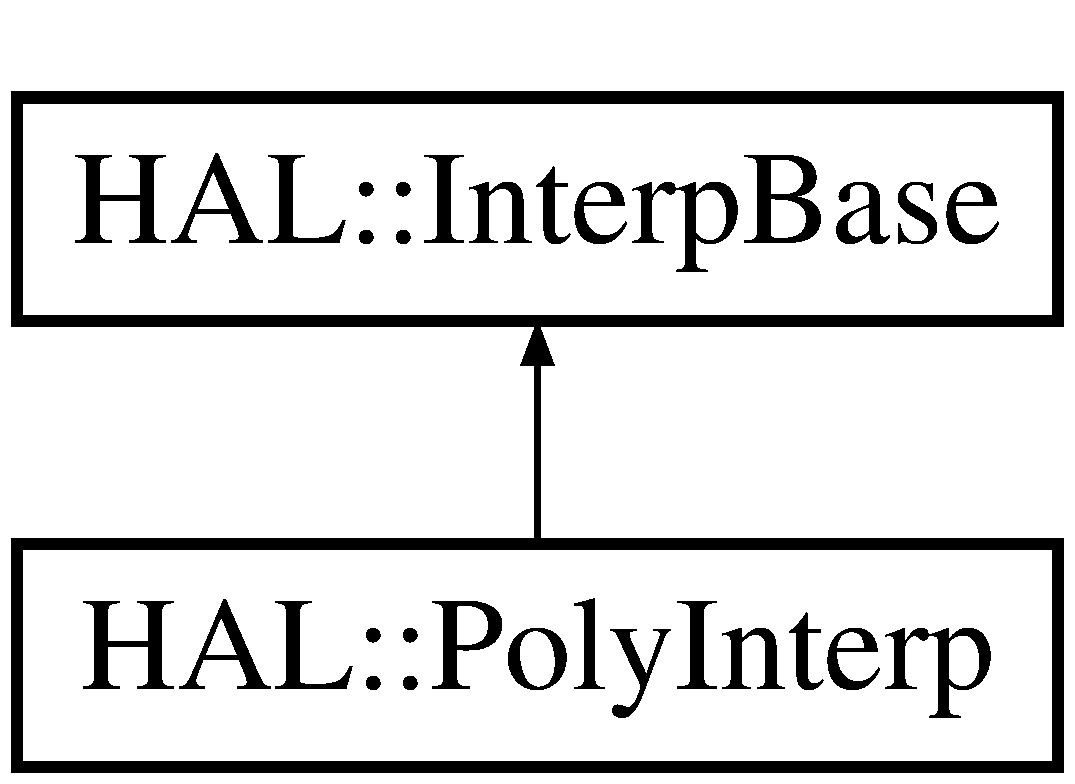
\includegraphics[height=2.000000cm]{class_h_a_l_1_1_interp_base}
\end{center}
\end{figure}
\subsection*{Public Member Functions}
\begin{DoxyCompactItemize}
\item 
\hypertarget{class_h_a_l_1_1_interp_base_a7da5f00617f93f337e983e48faa339d7}{{\bfseries Interp\+Base} (Double\+\_\+t $\ast$x, Double\+\_\+t $\ast$y, Int\+\_\+t xs, Int\+\_\+t m)}\label{class_h_a_l_1_1_interp_base_a7da5f00617f93f337e983e48faa339d7}

\item 
\hypertarget{class_h_a_l_1_1_interp_base_a54d32cf70679d2eb8d1a39a0bd242b39}{Int\+\_\+t {\bfseries locate} (const Double\+\_\+t \&x)}\label{class_h_a_l_1_1_interp_base_a54d32cf70679d2eb8d1a39a0bd242b39}

\item 
\hypertarget{class_h_a_l_1_1_interp_base_ad1bccffef0b532774150b419dbdff5b3}{Int\+\_\+t {\bfseries hunt} (const Double\+\_\+t \&x)}\label{class_h_a_l_1_1_interp_base_ad1bccffef0b532774150b419dbdff5b3}

\item 
\hypertarget{class_h_a_l_1_1_interp_base_a7d86cc16a9c8ba0bf24e8137f9eb21b3}{Double\+\_\+t {\bfseries Interp} (const Double\+\_\+t \&x)}\label{class_h_a_l_1_1_interp_base_a7d86cc16a9c8ba0bf24e8137f9eb21b3}

\item 
\hypertarget{class_h_a_l_1_1_interp_base_a524cc9b36f0e36c8f69f5c77bc68de7b}{virtual Double\+\_\+t {\bfseries rawinterp} (const Int\+\_\+t \&jlo, const Double\+\_\+t \&x)=0}\label{class_h_a_l_1_1_interp_base_a524cc9b36f0e36c8f69f5c77bc68de7b}

\end{DoxyCompactItemize}
\subsection*{Public Attributes}
\begin{DoxyCompactItemize}
\item 
\hypertarget{class_h_a_l_1_1_interp_base_a70c78b7c0ba2fe8a5ac3091ebb70f1ae}{Int\+\_\+t {\bfseries n}}\label{class_h_a_l_1_1_interp_base_a70c78b7c0ba2fe8a5ac3091ebb70f1ae}

\item 
\hypertarget{class_h_a_l_1_1_interp_base_a8691b520d0856373d8763be3cf0a9082}{Int\+\_\+t {\bfseries mm}}\label{class_h_a_l_1_1_interp_base_a8691b520d0856373d8763be3cf0a9082}

\item 
\hypertarget{class_h_a_l_1_1_interp_base_acfe70f15b2295e6b2399c02802072c9c}{Int\+\_\+t {\bfseries cor}}\label{class_h_a_l_1_1_interp_base_acfe70f15b2295e6b2399c02802072c9c}

\item 
\hypertarget{class_h_a_l_1_1_interp_base_a76921f15cd1908cdbe5bcc6afeb1ecc4}{Int\+\_\+t {\bfseries jsav}}\label{class_h_a_l_1_1_interp_base_a76921f15cd1908cdbe5bcc6afeb1ecc4}

\item 
\hypertarget{class_h_a_l_1_1_interp_base_af433768e4c59a1209919246ecb991c86}{Int\+\_\+t {\bfseries dj}}\label{class_h_a_l_1_1_interp_base_af433768e4c59a1209919246ecb991c86}

\item 
\hypertarget{class_h_a_l_1_1_interp_base_acdfb5ae98e96886c9055f36d29ebd25e}{Double\+\_\+t $\ast$ {\bfseries xx}}\label{class_h_a_l_1_1_interp_base_acdfb5ae98e96886c9055f36d29ebd25e}

\item 
\hypertarget{class_h_a_l_1_1_interp_base_a49d9cd794e1c97a0ed3f3bab3a999b8b}{Double\+\_\+t $\ast$ {\bfseries yy}}\label{class_h_a_l_1_1_interp_base_a49d9cd794e1c97a0ed3f3bab3a999b8b}

\end{DoxyCompactItemize}


The documentation for this class was generated from the following file\+:\begin{DoxyCompactItemize}
\item 
/\+Users/jhetherly/src/\+H\+A\+L-\/\+R\+O\+O\+T/include/\+H\+A\+L/Interpolator.\+h\end{DoxyCompactItemize}

\hypertarget{class_h_a_l_1_1_algorithms_1_1_min_chi_squared_selection}{\section{H\+A\+L\+:\+:Algorithms\+:\+:Min\+Chi\+Squared\+Selection Class Reference}
\label{class_h_a_l_1_1_algorithms_1_1_min_chi_squared_selection}\index{H\+A\+L\+::\+Algorithms\+::\+Min\+Chi\+Squared\+Selection@{H\+A\+L\+::\+Algorithms\+::\+Min\+Chi\+Squared\+Selection}}
}


\hyperlink{class_h_a_l_1_1_algorithm}{Algorithm} that performs a chi-\/squared minimization.  




{\ttfamily \#include $<$Min\+Chi\+Squared\+Selection.\+h$>$}

Inheritance diagram for H\+A\+L\+:\+:Algorithms\+:\+:Min\+Chi\+Squared\+Selection\+:\begin{figure}[H]
\begin{center}
\leavevmode
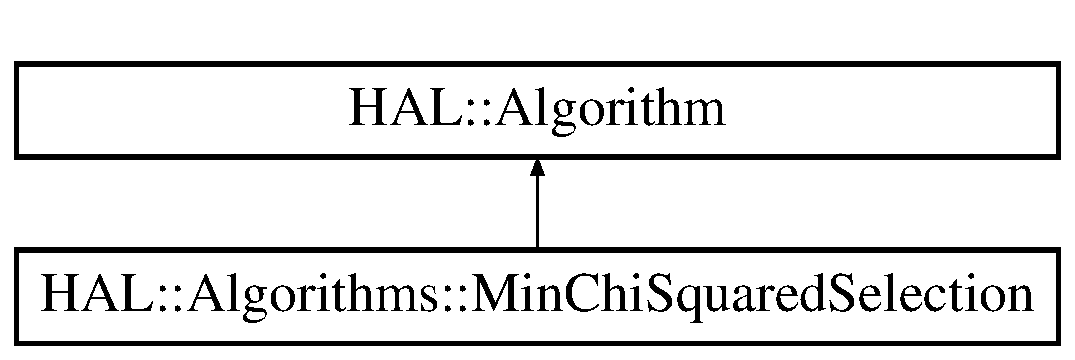
\includegraphics[height=2.000000cm]{class_h_a_l_1_1_algorithms_1_1_min_chi_squared_selection}
\end{center}
\end{figure}
\subsection*{Public Member Functions}
\begin{DoxyCompactItemize}
\item 
\hyperlink{class_h_a_l_1_1_algorithms_1_1_min_chi_squared_selection_a35bb157bbc031560febdbd377d94f429}{Min\+Chi\+Squared\+Selection} (T\+String name, T\+String title, long long nterms,...)
\begin{DoxyCompactList}\small\item\em Constructor. \end{DoxyCompactList}\end{DoxyCompactItemize}
\subsection*{Additional Inherited Members}


\subsection{Detailed Description}
\hyperlink{class_h_a_l_1_1_algorithm}{Algorithm} that performs a chi-\/squared minimization. 

This algorithm selects particles based on a chi-\/squared minimization. This algorithm properties are listed below. The particles from this algorithm are stored in many \hyperlink{class_h_a_l_1_1_generic_data}{Generic\+Data} object in the User\+Data under output names given to this algorithm's constructor.~\newline
~\newline
{\itshape Available Properties\+:} \begin{TabularC}{2}
\hline
\rowcolor{lightgray}\PBS\centering {\bf $ \Delta R $ }&\PBS\centering {\bf $ \Delta\phi $  }\\\cline{1-2}
\PBS\centering dr &\PBS\centering dphi \\\cline{1-2}
\end{TabularC}
{\bfseries Example\+:}~\newline
In your analysis file, do the following to select the jets within a $ \Delta R $ of 0.\+4 from the highest $ p_T $ jet\+:


\begin{DoxyCode}
\hyperlink{class_h_a_l_1_1_analysis}{HAL::Analysis} a(\textcolor{stringliteral}{"sample analysis"}, \textcolor{stringliteral}{""}, \textcolor{stringliteral}{"truth"});

a.AddAlgo(\textcolor{keyword}{new} \hyperlink{class_h_a_l_1_1_algorithms_1_1_import_particle}{HAL::Algorithms::ImportParticle}(\textcolor{stringliteral}{"jets"}, \textcolor{stringliteral}{"import basic jets"}));

\textcolor{comment}{//...}

a.AddAlgo(\textcolor{keyword}{new} \hyperlink{class_h_a_l_1_1_algorithms_1_1_particle_rank_selection}{HAL::Algorithms::ParticleRankSelection}(\textcolor{stringliteral}{"leading pt jet"}
      , \textcolor{stringliteral}{"find highest pt jet"}, 
                                                     \textcolor{stringliteral}{"jets"},
                                                     1, \textcolor{stringliteral}{"pt"}));

a.AddAlgo(\textcolor{keyword}{new} \hyperlink{class_h_a_l_1_1_algorithms_1_1_select_ref_particle}{HAL::Algorithms::SelectRefParticle}(\textcolor{stringliteral}{"jets close"}, \textcolor{stringliteral}{"filter on
       jets within deltaR of di-jet"}, 
                                                 \textcolor{stringliteral}{"leading pt jet"}, \textcolor{stringliteral}{"jets"},
                                                 0.4, \textcolor{stringliteral}{"dr"}));
\end{DoxyCode}
 

\subsection{Constructor \& Destructor Documentation}
\hypertarget{class_h_a_l_1_1_algorithms_1_1_min_chi_squared_selection_a35bb157bbc031560febdbd377d94f429}{\index{H\+A\+L\+::\+Algorithms\+::\+Min\+Chi\+Squared\+Selection@{H\+A\+L\+::\+Algorithms\+::\+Min\+Chi\+Squared\+Selection}!Min\+Chi\+Squared\+Selection@{Min\+Chi\+Squared\+Selection}}
\index{Min\+Chi\+Squared\+Selection@{Min\+Chi\+Squared\+Selection}!H\+A\+L\+::\+Algorithms\+::\+Min\+Chi\+Squared\+Selection@{H\+A\+L\+::\+Algorithms\+::\+Min\+Chi\+Squared\+Selection}}
\subsubsection[{Min\+Chi\+Squared\+Selection}]{\setlength{\rightskip}{0pt plus 5cm}H\+A\+L\+::\+Algorithms\+::\+Min\+Chi\+Squared\+Selection\+::\+Min\+Chi\+Squared\+Selection (
\begin{DoxyParamCaption}
\item[{T\+String}]{name, }
\item[{T\+String}]{title, }
\item[{long long}]{nterms, }
\item[{}]{...}
\end{DoxyParamCaption}
)}}\label{class_h_a_l_1_1_algorithms_1_1_min_chi_squared_selection_a35bb157bbc031560febdbd377d94f429}


Constructor. 

Initializes the algorithm. The variable length argument at the end should conform to the following rules\+:~\newline

\begin{DoxyItemize}
\item It should be given in sets of seven.
\item The first
\item The second
\item The third
\item The fourth
\item The fifth
\item The sixth
\item The seventh
\end{DoxyItemize}


\begin{DoxyParams}[1]{Parameters}
\mbox{\tt in}  & {\em name} & Name of the algorithm. This can be used as the input to other algorithms. \\
\hline
\mbox{\tt in}  & {\em title} & Description of the algorithm. Can be an empty string. \\
\hline
\mbox{\tt in}  & {\em nterms} & Number of cuts to make. \\
\hline
\mbox{\tt in}  & {\em ...} & Set of seven values per term as explained above. \\
\hline
\end{DoxyParams}
\begin{DoxySeeAlso}{See also}

\end{DoxySeeAlso}


The documentation for this class was generated from the following file\+:\begin{DoxyCompactItemize}
\item 
/\+Users/jhetherly/src/\+H\+A\+L-\/\+R\+O\+O\+T/include/\+H\+A\+L/\+Algorithms/\hyperlink{_min_chi_squared_selection_8h}{Min\+Chi\+Squared\+Selection.\+h}\end{DoxyCompactItemize}

\hypertarget{class_h_a_l_1_1_algorithms_1_1_monitor_algorithm}{\section{H\+A\+L\+:\+:Algorithms\+:\+:Monitor\+Algorithm Class Reference}
\label{class_h_a_l_1_1_algorithms_1_1_monitor_algorithm}\index{H\+A\+L\+::\+Algorithms\+::\+Monitor\+Algorithm@{H\+A\+L\+::\+Algorithms\+::\+Monitor\+Algorithm}}
}


Generic algorithm class that prints the content of an algorithm to a given ostream.  




{\ttfamily \#include $<$Monitor.\+h$>$}

Inheritance diagram for H\+A\+L\+:\+:Algorithms\+:\+:Monitor\+Algorithm\+:\begin{figure}[H]
\begin{center}
\leavevmode
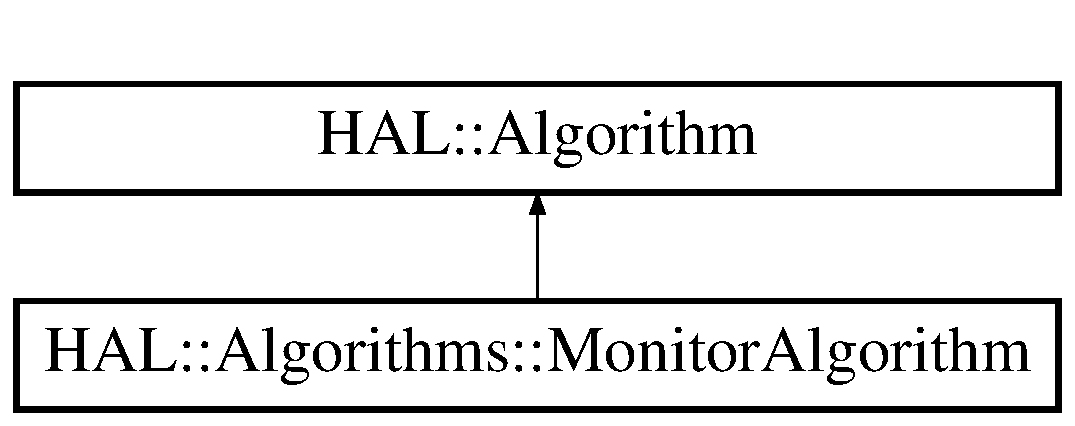
\includegraphics[height=2.000000cm]{class_h_a_l_1_1_algorithms_1_1_monitor_algorithm}
\end{center}
\end{figure}
\subsection*{Public Member Functions}
\begin{DoxyCompactItemize}
\item 
\hyperlink{class_h_a_l_1_1_algorithms_1_1_monitor_algorithm_ac37ea6c50b23dbb49b63d9fe551554a7}{Monitor\+Algorithm} (T\+String name, T\+String title, T\+String input, long long period=1, std\+::ostream \&os=std\+::cout)
\begin{DoxyCompactList}\small\item\em Constructor. \end{DoxyCompactList}\end{DoxyCompactItemize}
\subsection*{Protected Member Functions}
\begin{DoxyCompactItemize}
\item 
\hypertarget{class_h_a_l_1_1_algorithms_1_1_monitor_algorithm_ae1efc679e7dcbc8692a6b37dca0517c3}{virtual void {\bfseries Exec} (Option\+\_\+t $\ast$)}\label{class_h_a_l_1_1_algorithms_1_1_monitor_algorithm_ae1efc679e7dcbc8692a6b37dca0517c3}

\end{DoxyCompactItemize}
\subsection*{Additional Inherited Members}


\subsection{Detailed Description}
Generic algorithm class that prints the content of an algorithm to a given ostream. 

This algorithm is helpful in monitoring the particles produced or value stored by another generic algorithm. {\bfseries Example\+:}~\newline
In your analysis file, do the following to monitor the output of an algorithm\+:


\begin{DoxyCode}
\hyperlink{class_h_a_l_1_1_analysis}{HAL::Analysis} a(\textcolor{stringliteral}{"sample analysis"}, \textcolor{stringliteral}{""}, \textcolor{stringliteral}{"truth"});

a.AddAlgo(\textcolor{keyword}{new} \hyperlink{class_h_a_l_1_1_algorithms_1_1_import_particle}{HAL::Algorithms::ImportParticle}(\textcolor{stringliteral}{"jets"}, \textcolor{stringliteral}{"import basic jet
       objects"}));

a.AddAlgo(\textcolor{keyword}{new} \hyperlink{class_h_a_l_1_1_algorithms_1_1_particle_rank_selection}{HAL::Algorithms::ParticleRankSelection}(\textcolor{stringliteral}{"leading pt jet"}
      , \textcolor{stringliteral}{"find highest pt jet"}, 
                                                     \textcolor{stringliteral}{"jets"},
                                                     1, \textcolor{stringliteral}{"pt"}));

a.AddAlgo(\textcolor{keyword}{new} \hyperlink{class_h_a_l_1_1_algorithms_1_1_monitor_algorithm}{HAL::Algorithms::MonitorAlgorithm}(\textcolor{stringliteral}{"leading jet monitor"}, \textcolor{stringliteral}{"
      look at the leading jet"}, 
                                                \textcolor{stringliteral}{"leading pt jet"}, 100));
\end{DoxyCode}
 

\subsection{Constructor \& Destructor Documentation}
\hypertarget{class_h_a_l_1_1_algorithms_1_1_monitor_algorithm_ac37ea6c50b23dbb49b63d9fe551554a7}{\index{H\+A\+L\+::\+Algorithms\+::\+Monitor\+Algorithm@{H\+A\+L\+::\+Algorithms\+::\+Monitor\+Algorithm}!Monitor\+Algorithm@{Monitor\+Algorithm}}
\index{Monitor\+Algorithm@{Monitor\+Algorithm}!H\+A\+L\+::\+Algorithms\+::\+Monitor\+Algorithm@{H\+A\+L\+::\+Algorithms\+::\+Monitor\+Algorithm}}
\subsubsection[{Monitor\+Algorithm}]{\setlength{\rightskip}{0pt plus 5cm}H\+A\+L\+::\+Algorithms\+::\+Monitor\+Algorithm\+::\+Monitor\+Algorithm (
\begin{DoxyParamCaption}
\item[{T\+String}]{name, }
\item[{T\+String}]{title, }
\item[{T\+String}]{input, }
\item[{long long}]{period = {\ttfamily 1}, }
\item[{std\+::ostream \&}]{os = {\ttfamily std\+:\+:cout}}
\end{DoxyParamCaption}
)\hspace{0.3cm}{\ttfamily [inline]}}}\label{class_h_a_l_1_1_algorithms_1_1_monitor_algorithm_ac37ea6c50b23dbb49b63d9fe551554a7}


Constructor. 

Initializes the algorithm. 
\begin{DoxyParams}[1]{Parameters}
\mbox{\tt in}  & {\em name} & Name of the algorithm. This can be used as the input to other algorithms. \\
\hline
\mbox{\tt in}  & {\em title} & Description of the algorithm. Can be an empty string. \\
\hline
\mbox{\tt in}  & {\em input} & Name of algorithm to select from. \\
\hline
\mbox{\tt in}  & {\em period} & Sets the period of output. \\
\hline
\mbox{\tt in}  & {\em os} & Stream to pipe all output to. \\
\hline
\end{DoxyParams}


The documentation for this class was generated from the following file\+:\begin{DoxyCompactItemize}
\item 
/\+Users/jhetherly/src/\+H\+A\+L-\/\+R\+O\+O\+T/include/\+H\+A\+L/\+Algorithms/\hyperlink{_monitor_8h}{Monitor.\+h}\end{DoxyCompactItemize}

\hypertarget{class_h_a_l_1_1_algorithms_1_1_monitor_user_data}{\section{H\+A\+L\+:\+:Algorithms\+:\+:Monitor\+User\+Data Class Reference}
\label{class_h_a_l_1_1_algorithms_1_1_monitor_user_data}\index{H\+A\+L\+::\+Algorithms\+::\+Monitor\+User\+Data@{H\+A\+L\+::\+Algorithms\+::\+Monitor\+User\+Data}}
}
Inheritance diagram for H\+A\+L\+:\+:Algorithms\+:\+:Monitor\+User\+Data\+:\begin{figure}[H]
\begin{center}
\leavevmode
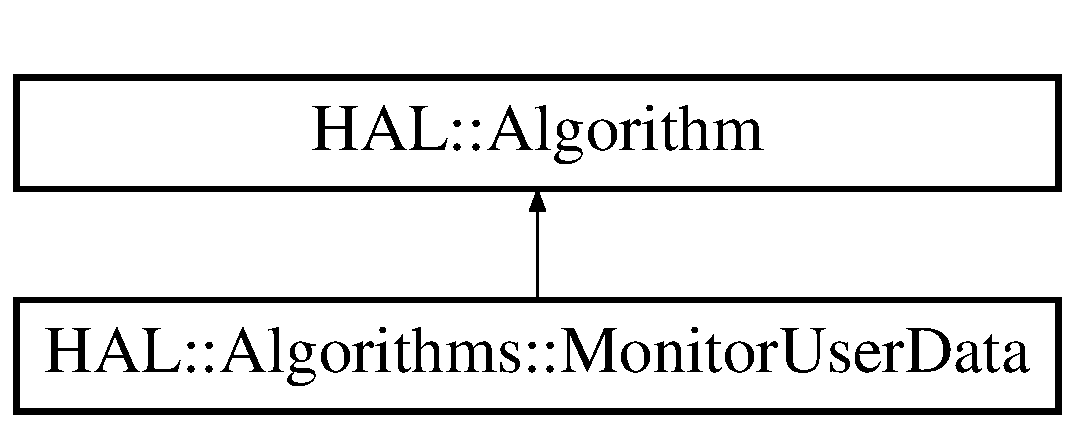
\includegraphics[height=2.000000cm]{class_h_a_l_1_1_algorithms_1_1_monitor_user_data}
\end{center}
\end{figure}
\subsection*{Public Member Functions}
\begin{DoxyCompactItemize}
\item 
\hypertarget{class_h_a_l_1_1_algorithms_1_1_monitor_user_data_acd4eeebf53037457c4b0e2095934a723}{{\bfseries Monitor\+User\+Data} (T\+String name, T\+String title, std\+::ostream \&os=std\+::cout)}\label{class_h_a_l_1_1_algorithms_1_1_monitor_user_data_acd4eeebf53037457c4b0e2095934a723}

\end{DoxyCompactItemize}
\subsection*{Protected Member Functions}
\begin{DoxyCompactItemize}
\item 
virtual void \hyperlink{class_h_a_l_1_1_algorithms_1_1_monitor_user_data_aea4229dea8ffbd7edfa8a4108e72205c}{Exec} (Option\+\_\+t $\ast$)
\begin{DoxyCompactList}\small\item\em Hook into the T\+Selector\+::\+Process method. \end{DoxyCompactList}\end{DoxyCompactItemize}
\subsection*{Additional Inherited Members}


\subsection{Member Function Documentation}
\hypertarget{class_h_a_l_1_1_algorithms_1_1_monitor_user_data_aea4229dea8ffbd7edfa8a4108e72205c}{\index{H\+A\+L\+::\+Algorithms\+::\+Monitor\+User\+Data@{H\+A\+L\+::\+Algorithms\+::\+Monitor\+User\+Data}!Exec@{Exec}}
\index{Exec@{Exec}!H\+A\+L\+::\+Algorithms\+::\+Monitor\+User\+Data@{H\+A\+L\+::\+Algorithms\+::\+Monitor\+User\+Data}}
\subsubsection[{Exec}]{\setlength{\rightskip}{0pt plus 5cm}virtual void H\+A\+L\+::\+Algorithms\+::\+Monitor\+User\+Data\+::\+Exec (
\begin{DoxyParamCaption}
\item[{Option\+\_\+t $\ast$}]{}
\end{DoxyParamCaption}
)\hspace{0.3cm}{\ttfamily [protected]}, {\ttfamily [virtual]}}}\label{class_h_a_l_1_1_algorithms_1_1_monitor_user_data_aea4229dea8ffbd7edfa8a4108e72205c}


Hook into the T\+Selector\+::\+Process method. 

This method allows the algorithm operate at the first part of the 'Process' stage of processing a T\+Tree. This where most of the logic of an algorithm will likely be contained. 
\begin{DoxyParams}[1]{Parameters}
\mbox{\tt in}  & {\em option} & Option string passed to all algorithms from the Analysis\+::\+Process call \\
\hline
\end{DoxyParams}


Reimplemented from \hyperlink{class_h_a_l_1_1_algorithm_a438c5c54698aa014b660474d08703bc2}{H\+A\+L\+::\+Algorithm}.



The documentation for this class was generated from the following file\+:\begin{DoxyCompactItemize}
\item 
/\+Users/jhetherly/src/\+H\+A\+L-\/\+R\+O\+O\+T/include/\+H\+A\+L/\+Algorithms/\hyperlink{_monitor_8h}{Monitor.\+h}\end{DoxyCompactItemize}

\hypertarget{class_h_a_l_1_1_algorithms_1_1_particle_rank_selection}{\section{H\+A\+L\+:\+:Algorithms\+:\+:Particle\+Rank\+Selection Class Reference}
\label{class_h_a_l_1_1_algorithms_1_1_particle_rank_selection}\index{H\+A\+L\+::\+Algorithms\+::\+Particle\+Rank\+Selection@{H\+A\+L\+::\+Algorithms\+::\+Particle\+Rank\+Selection}}
}


\hyperlink{class_h_a_l_1_1_algorithm}{Algorithm} that selects the particle with the highest or lowest property.  




{\ttfamily \#include $<$Particle\+Rank\+Selection.\+h$>$}

Inheritance diagram for H\+A\+L\+:\+:Algorithms\+:\+:Particle\+Rank\+Selection\+:\begin{figure}[H]
\begin{center}
\leavevmode
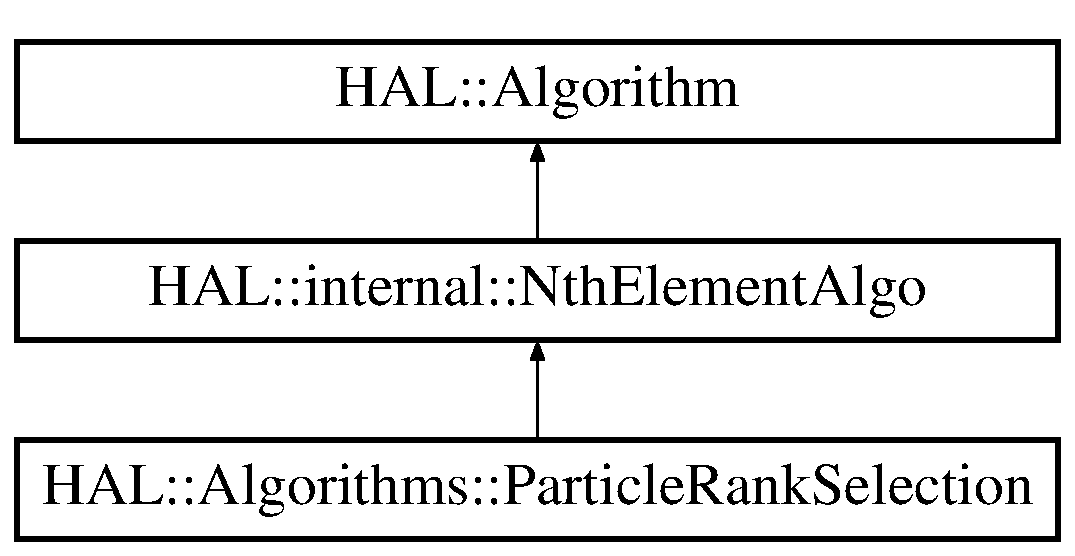
\includegraphics[height=3.000000cm]{class_h_a_l_1_1_algorithms_1_1_particle_rank_selection}
\end{center}
\end{figure}
\subsection*{Public Member Functions}
\begin{DoxyCompactItemize}
\item 
\hyperlink{class_h_a_l_1_1_algorithms_1_1_particle_rank_selection_acbba84c85f7090200eda0d2a0bd9c677}{Particle\+Rank\+Selection} (T\+String name, T\+String title, T\+String input, unsigned rank, T\+String property, T\+String end=\char`\"{}high\char`\"{})
\begin{DoxyCompactList}\small\item\em Constructor. \end{DoxyCompactList}\item 
\hypertarget{class_h_a_l_1_1_algorithms_1_1_particle_rank_selection_acce9ba5e039ebd2040b5f7172586e5b1}{virtual T\+String {\bfseries Sort\+Tag} ()}\label{class_h_a_l_1_1_algorithms_1_1_particle_rank_selection_acce9ba5e039ebd2040b5f7172586e5b1}

\item 
\hypertarget{class_h_a_l_1_1_algorithms_1_1_particle_rank_selection_ac1e2275f72f43fd1e80fdbdefbfe9aaf}{virtual bool {\bfseries operator()} (\hyperlink{class_h_a_l_1_1_generic_particle}{Particle\+Ptr}, \hyperlink{class_h_a_l_1_1_generic_particle}{Particle\+Ptr})}\label{class_h_a_l_1_1_algorithms_1_1_particle_rank_selection_ac1e2275f72f43fd1e80fdbdefbfe9aaf}

\item 
\hypertarget{class_h_a_l_1_1_algorithms_1_1_particle_rank_selection_a0519f017f9142ce0d484b3e99f70aa19}{virtual void {\bfseries Sort} (Particle\+Ptrs \&)}\label{class_h_a_l_1_1_algorithms_1_1_particle_rank_selection_a0519f017f9142ce0d484b3e99f70aa19}

\end{DoxyCompactItemize}
\subsection*{Protected Attributes}
\begin{DoxyCompactItemize}
\item 
\hypertarget{class_h_a_l_1_1_algorithms_1_1_particle_rank_selection_a57e25ecd8df075abefc0513d3fd4f35d}{bool {\bfseries f\+Pt}}\label{class_h_a_l_1_1_algorithms_1_1_particle_rank_selection_a57e25ecd8df075abefc0513d3fd4f35d}

\item 
\hypertarget{class_h_a_l_1_1_algorithms_1_1_particle_rank_selection_a9a058d0591d0af0117902b3afbe1f3a1}{bool {\bfseries f\+M}}\label{class_h_a_l_1_1_algorithms_1_1_particle_rank_selection_a9a058d0591d0af0117902b3afbe1f3a1}

\item 
\hypertarget{class_h_a_l_1_1_algorithms_1_1_particle_rank_selection_a47f5390942d104168c66f2db36de5be7}{bool {\bfseries f\+E}}\label{class_h_a_l_1_1_algorithms_1_1_particle_rank_selection_a47f5390942d104168c66f2db36de5be7}

\item 
\hypertarget{class_h_a_l_1_1_algorithms_1_1_particle_rank_selection_a61ee40fd1634b4c781d28c2cdd0cd794}{bool {\bfseries f\+Et}}\label{class_h_a_l_1_1_algorithms_1_1_particle_rank_selection_a61ee40fd1634b4c781d28c2cdd0cd794}

\item 
\hypertarget{class_h_a_l_1_1_algorithms_1_1_particle_rank_selection_aca51ef5461c379d4e0ac859c9206f574}{bool {\bfseries f\+P3}}\label{class_h_a_l_1_1_algorithms_1_1_particle_rank_selection_aca51ef5461c379d4e0ac859c9206f574}

\item 
\hypertarget{class_h_a_l_1_1_algorithms_1_1_particle_rank_selection_a14c9adc724ebf5f7b3fc22f123ea3298}{bool {\bfseries f\+High}}\label{class_h_a_l_1_1_algorithms_1_1_particle_rank_selection_a14c9adc724ebf5f7b3fc22f123ea3298}

\item 
\hypertarget{class_h_a_l_1_1_algorithms_1_1_particle_rank_selection_a701d83445ff240dae44927141eb4c7be}{bool {\bfseries f\+Low}}\label{class_h_a_l_1_1_algorithms_1_1_particle_rank_selection_a701d83445ff240dae44927141eb4c7be}

\item 
\hypertarget{class_h_a_l_1_1_algorithms_1_1_particle_rank_selection_aea4217b70b01d2f4b3d0f0566ea48c89}{T\+String {\bfseries f\+T\+L\+V\+Property}}\label{class_h_a_l_1_1_algorithms_1_1_particle_rank_selection_aea4217b70b01d2f4b3d0f0566ea48c89}

\item 
\hypertarget{class_h_a_l_1_1_algorithms_1_1_particle_rank_selection_a9bdf92cec167ae6f9a42cf951117efe3}{T\+String {\bfseries f\+End}}\label{class_h_a_l_1_1_algorithms_1_1_particle_rank_selection_a9bdf92cec167ae6f9a42cf951117efe3}

\end{DoxyCompactItemize}


\subsection{Detailed Description}
\hyperlink{class_h_a_l_1_1_algorithm}{Algorithm} that selects the particle with the highest or lowest property. 

This algorithm selects the particle with highest or lowest property. The list of available properties is given below. A property is input as a string to the constructor of this algorithm. The particle from this algorithm is stored in a \hyperlink{class_h_a_l_1_1_generic_data}{Generic\+Data} object in the User\+Data under the algorithm's name.~\newline
~\newline
{\itshape Available Properties\+:} \begin{TabularC}{5}
\hline
\rowcolor{lightgray}\PBS\centering {\bf $ p_T $ }&\PBS\centering {\bf $ E_T $ }&\PBS\centering {\bf Mass }&\PBS\centering {\bf Energy }&\PBS\centering {\bf $ \left|\overrightarrow{p}\right| $  }\\\cline{1-5}
\PBS\centering p\+T &\PBS\centering e\+T &\PBS\centering m &\PBS\centering e &\PBS\centering p3 \\\cline{1-5}
\end{TabularC}
{\bfseries Example\+:}~\newline
In your analysis file, do the following to select the highest $ p_T $ muon\+:


\begin{DoxyCode}
\hyperlink{class_h_a_l_1_1_analysis}{HAL::Analysis} a(\textcolor{stringliteral}{"sample analysis"}, \textcolor{stringliteral}{""}, \textcolor{stringliteral}{"truth"});

a.AddAlgo(\textcolor{keyword}{new} \hyperlink{class_h_a_l_1_1_algorithms_1_1_import_particle}{HAL::Algorithms::ImportParticle}(\textcolor{stringliteral}{"muons"}, \textcolor{stringliteral}{"import basic muons"})
      );

\textcolor{comment}{//...}

a.AddAlgo(\textcolor{keyword}{new} \hyperlink{class_h_a_l_1_1_algorithms_1_1_particle_rank_selection}{HAL::Algorithms::ParticleRankSelection}(\textcolor{stringliteral}{"highest pT muon
      "}, \textcolor{stringliteral}{"find highest pT muon"}, 
                                                     \textcolor{stringliteral}{"muons"}, 1, \textcolor{stringliteral}{"pT"}, \textcolor{stringliteral}{"high"}));
\end{DoxyCode}
 

\subsection{Constructor \& Destructor Documentation}
\hypertarget{class_h_a_l_1_1_algorithms_1_1_particle_rank_selection_acbba84c85f7090200eda0d2a0bd9c677}{\index{H\+A\+L\+::\+Algorithms\+::\+Particle\+Rank\+Selection@{H\+A\+L\+::\+Algorithms\+::\+Particle\+Rank\+Selection}!Particle\+Rank\+Selection@{Particle\+Rank\+Selection}}
\index{Particle\+Rank\+Selection@{Particle\+Rank\+Selection}!H\+A\+L\+::\+Algorithms\+::\+Particle\+Rank\+Selection@{H\+A\+L\+::\+Algorithms\+::\+Particle\+Rank\+Selection}}
\subsubsection[{Particle\+Rank\+Selection}]{\setlength{\rightskip}{0pt plus 5cm}H\+A\+L\+::\+Algorithms\+::\+Particle\+Rank\+Selection\+::\+Particle\+Rank\+Selection (
\begin{DoxyParamCaption}
\item[{T\+String}]{name, }
\item[{T\+String}]{title, }
\item[{T\+String}]{input, }
\item[{unsigned}]{rank, }
\item[{T\+String}]{property, }
\item[{T\+String}]{end = {\ttfamily \char`\"{}high\char`\"{}}}
\end{DoxyParamCaption}
)}}\label{class_h_a_l_1_1_algorithms_1_1_particle_rank_selection_acbba84c85f7090200eda0d2a0bd9c677}


Constructor. 

Initializes the algorithm 
\begin{DoxyParams}[1]{Parameters}
\mbox{\tt in}  & {\em name} & Name of the algorithm. This can be used as the input to other algorithms. \\
\hline
\mbox{\tt in}  & {\em title} & Description of the algorithm. Can be an empty string. \\
\hline
\mbox{\tt in}  & {\em input} & Name of algorithm to select from. \\
\hline
\mbox{\tt in}  & {\em rank} & Rank of particle. \\
\hline
\mbox{\tt in}  & {\em property} & Property to rank particle by. \\
\hline
\mbox{\tt in}  & {\em end} & Either \char`\"{}high\char`\"{} for highest rank property or \char`\"{}low\char`\"{} for lowest rank property. \\
\hline
\end{DoxyParams}
\begin{DoxySeeAlso}{See also}
\hyperlink{class_h_a_l_1_1_algorithms_1_1_import_particle}{Import\+Particle}, \hyperlink{class_h_a_l_1_1_algorithms_1_1_select_particle}{Select\+Particle} 
\end{DoxySeeAlso}


The documentation for this class was generated from the following file\+:\begin{DoxyCompactItemize}
\item 
/\+Users/jhetherly/src/\+H\+A\+L-\/\+R\+O\+O\+T/include/\+H\+A\+L/\+Algorithms/\hyperlink{_particle_rank_selection_8h}{Particle\+Rank\+Selection.\+h}\end{DoxyCompactItemize}

\hypertarget{class_h_a_l_1_1_poly2_d_interp}{\section{H\+A\+L\+:\+:Poly2\+D\+Interp Class Reference}
\label{class_h_a_l_1_1_poly2_d_interp}\index{H\+A\+L\+::\+Poly2\+D\+Interp@{H\+A\+L\+::\+Poly2\+D\+Interp}}
}
\subsection*{Public Member Functions}
\begin{DoxyCompactItemize}
\item 
\hypertarget{class_h_a_l_1_1_poly2_d_interp_a2e06fafe80eb98739813a67a1f5b5f89}{{\bfseries Poly2\+D\+Interp} (Double\+\_\+t $\ast$x1\+\_\+values, Double\+\_\+t $\ast$x2\+\_\+values, Int\+\_\+t x1\+\_\+size, Int\+\_\+t x2\+\_\+size, Double\+\_\+t $\ast$$\ast$y\+\_\+matrix, Int\+\_\+t x1\+\_\+order, Int\+\_\+t x2\+\_\+order)}\label{class_h_a_l_1_1_poly2_d_interp_a2e06fafe80eb98739813a67a1f5b5f89}

\item 
\hypertarget{class_h_a_l_1_1_poly2_d_interp_aaeda2c3c4e09d48611973dcd95940756}{Double\+\_\+t {\bfseries Interp} (const Double\+\_\+t \&x1\+\_\+value, const Double\+\_\+t \&x2\+\_\+value)}\label{class_h_a_l_1_1_poly2_d_interp_aaeda2c3c4e09d48611973dcd95940756}

\item 
\hypertarget{class_h_a_l_1_1_poly2_d_interp_a3488ef8691d670a5f2170a9ebead44d7}{Double\+\_\+t {\bfseries Get\+X1\+Error} ()}\label{class_h_a_l_1_1_poly2_d_interp_a3488ef8691d670a5f2170a9ebead44d7}

\item 
\hypertarget{class_h_a_l_1_1_poly2_d_interp_a9d7ab5e66ee29fe41187d39086152dfe}{Double\+\_\+t {\bfseries Get\+X2\+Error} ()}\label{class_h_a_l_1_1_poly2_d_interp_a9d7ab5e66ee29fe41187d39086152dfe}

\end{DoxyCompactItemize}
\subsection*{Public Attributes}
\begin{DoxyCompactItemize}
\item 
\hypertarget{class_h_a_l_1_1_poly2_d_interp_af07844f91abbfa62348292ae16a90fdc}{Double\+\_\+t $\ast$$\ast$ {\bfseries y}}\label{class_h_a_l_1_1_poly2_d_interp_af07844f91abbfa62348292ae16a90fdc}

\end{DoxyCompactItemize}


The documentation for this class was generated from the following file\+:\begin{DoxyCompactItemize}
\item 
/\+Users/jhetherly/src/root\+\_\+\+H\+A\+L/include/\+H\+A\+L/Interpolator.\+h\end{DoxyCompactItemize}

\hypertarget{class_h_a_l_1_1_poly_interp}{\section{H\+A\+L\+:\+:Poly\+Interp Class Reference}
\label{class_h_a_l_1_1_poly_interp}\index{H\+A\+L\+::\+Poly\+Interp@{H\+A\+L\+::\+Poly\+Interp}}
}
Inheritance diagram for H\+A\+L\+:\+:Poly\+Interp\+:\begin{figure}[H]
\begin{center}
\leavevmode
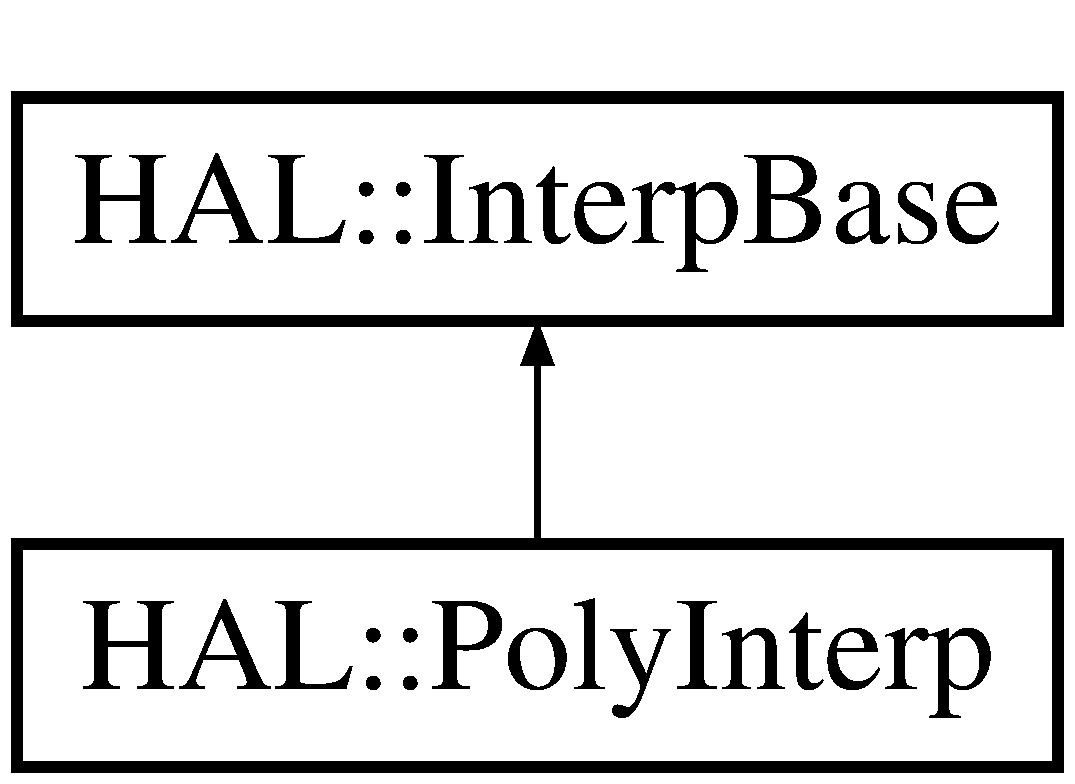
\includegraphics[height=2.000000cm]{class_h_a_l_1_1_poly_interp}
\end{center}
\end{figure}
\subsection*{Public Member Functions}
\begin{DoxyCompactItemize}
\item 
\hypertarget{class_h_a_l_1_1_poly_interp_af44f92e27052c066755a5beae2dc7b1b}{{\bfseries Poly\+Interp} (Double\+\_\+t $\ast$x\+\_\+values, Double\+\_\+t $\ast$y\+\_\+values, Int\+\_\+t size, Int\+\_\+t order)}\label{class_h_a_l_1_1_poly_interp_af44f92e27052c066755a5beae2dc7b1b}

\item 
\hypertarget{class_h_a_l_1_1_poly_interp_a1d87892f07ecdacaf6467a63371f044e}{Double\+\_\+t {\bfseries Get\+Error} ()}\label{class_h_a_l_1_1_poly_interp_a1d87892f07ecdacaf6467a63371f044e}

\end{DoxyCompactItemize}
\subsection*{Friends}
\begin{DoxyCompactItemize}
\item 
\hypertarget{class_h_a_l_1_1_poly_interp_a1d517ab352221a0d0a7fbfc8698724d7}{class {\bfseries Poly2\+D\+Interp}}\label{class_h_a_l_1_1_poly_interp_a1d517ab352221a0d0a7fbfc8698724d7}

\end{DoxyCompactItemize}
\subsection*{Additional Inherited Members}


The documentation for this class was generated from the following file\+:\begin{DoxyCompactItemize}
\item 
/\+Users/jhetherly/src/\+H\+A\+L-\/\+R\+O\+O\+T/include/\+H\+A\+L/Interpolator.\+h\end{DoxyCompactItemize}

\hypertarget{class_h_a_l_1_1_python_algorithm}{\section{H\+A\+L\+:\+:Python\+Algorithm Class Reference}
\label{class_h_a_l_1_1_python_algorithm}\index{H\+A\+L\+::\+Python\+Algorithm@{H\+A\+L\+::\+Python\+Algorithm}}
}
Inheritance diagram for H\+A\+L\+:\+:Python\+Algorithm\+:\begin{figure}[H]
\begin{center}
\leavevmode
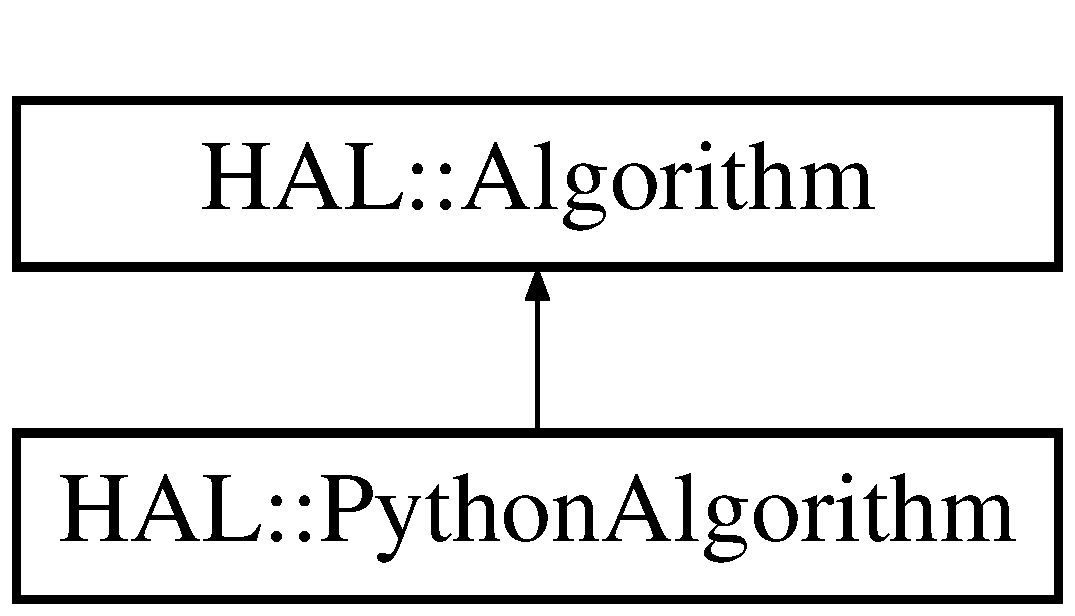
\includegraphics[height=2.000000cm]{class_h_a_l_1_1_python_algorithm}
\end{center}
\end{figure}
\subsection*{Public Member Functions}
\begin{DoxyCompactItemize}
\item 
\hypertarget{class_h_a_l_1_1_python_algorithm_a91ca9d7b2a002013b5dd27951aca3678}{{\bfseries Python\+Algorithm} (T\+String name=\char`\"{}\char`\"{}, T\+String title=\char`\"{}\char`\"{}, T\+String Py\+Path=\char`\"{}\char`\"{}, T\+String Py\+File=\char`\"{}\char`\"{}, T\+String Py\+Class=\char`\"{}\char`\"{}, Py\+Object $\ast$self=0)}\label{class_h_a_l_1_1_python_algorithm_a91ca9d7b2a002013b5dd27951aca3678}

\item 
virtual void \hyperlink{class_h_a_l_1_1_python_algorithm_a951c827d0f926b5096f7e59accc1e007}{Init} (Option\+\_\+t $\ast$options=\char`\"{}\char`\"{})
\begin{DoxyCompactList}\small\item\em Hook into the T\+Selector\+::\+Init method. \end{DoxyCompactList}\item 
virtual void \hyperlink{class_h_a_l_1_1_python_algorithm_a64a70202dd5da390ab6654a7e33c5976}{Exec} (Option\+\_\+t $\ast$options=\char`\"{}\char`\"{})
\begin{DoxyCompactList}\small\item\em Hook into the T\+Selector\+::\+Process method. \end{DoxyCompactList}\item 
virtual void \hyperlink{class_h_a_l_1_1_python_algorithm_aac72e398eadd979cf62617fe2fbe1a01}{Clear} (Option\+\_\+t $\ast$options=\char`\"{}\char`\"{})
\begin{DoxyCompactList}\small\item\em Hook into the T\+Selector\+::\+Process method. \end{DoxyCompactList}\end{DoxyCompactItemize}
\subsection*{Additional Inherited Members}


\subsection{Member Function Documentation}
\hypertarget{class_h_a_l_1_1_python_algorithm_aac72e398eadd979cf62617fe2fbe1a01}{\index{H\+A\+L\+::\+Python\+Algorithm@{H\+A\+L\+::\+Python\+Algorithm}!Clear@{Clear}}
\index{Clear@{Clear}!H\+A\+L\+::\+Python\+Algorithm@{H\+A\+L\+::\+Python\+Algorithm}}
\subsubsection[{Clear}]{\setlength{\rightskip}{0pt plus 5cm}virtual void H\+A\+L\+::\+Python\+Algorithm\+::\+Clear (
\begin{DoxyParamCaption}
\item[{Option\+\_\+t $\ast$}]{ = {\ttfamily \char`\"{}\char`\"{}}}
\end{DoxyParamCaption}
)\hspace{0.3cm}{\ttfamily [virtual]}}}\label{class_h_a_l_1_1_python_algorithm_aac72e398eadd979cf62617fe2fbe1a01}


Hook into the T\+Selector\+::\+Process method. 

This method allows the algorithm operate at the second part of the 'Process' stage of processing a T\+Tree. This is meant for any per-\/event memory management. 
\begin{DoxyParams}[1]{Parameters}
\mbox{\tt in}  & {\em option} & Option string passed to all algorithms from the Analysis\+::\+Process call \\
\hline
\end{DoxyParams}


Reimplemented from \hyperlink{class_h_a_l_1_1_algorithm_a2a26a5549e92efaa968763ac51e6758a}{H\+A\+L\+::\+Algorithm}.

\hypertarget{class_h_a_l_1_1_python_algorithm_a64a70202dd5da390ab6654a7e33c5976}{\index{H\+A\+L\+::\+Python\+Algorithm@{H\+A\+L\+::\+Python\+Algorithm}!Exec@{Exec}}
\index{Exec@{Exec}!H\+A\+L\+::\+Python\+Algorithm@{H\+A\+L\+::\+Python\+Algorithm}}
\subsubsection[{Exec}]{\setlength{\rightskip}{0pt plus 5cm}virtual void H\+A\+L\+::\+Python\+Algorithm\+::\+Exec (
\begin{DoxyParamCaption}
\item[{Option\+\_\+t $\ast$}]{ = {\ttfamily \char`\"{}\char`\"{}}}
\end{DoxyParamCaption}
)\hspace{0.3cm}{\ttfamily [virtual]}}}\label{class_h_a_l_1_1_python_algorithm_a64a70202dd5da390ab6654a7e33c5976}


Hook into the T\+Selector\+::\+Process method. 

This method allows the algorithm operate at the first part of the 'Process' stage of processing a T\+Tree. This where most of the logic of an algorithm will likely be contained. 
\begin{DoxyParams}[1]{Parameters}
\mbox{\tt in}  & {\em option} & Option string passed to all algorithms from the Analysis\+::\+Process call \\
\hline
\end{DoxyParams}


Reimplemented from \hyperlink{class_h_a_l_1_1_algorithm_a438c5c54698aa014b660474d08703bc2}{H\+A\+L\+::\+Algorithm}.

\hypertarget{class_h_a_l_1_1_python_algorithm_a951c827d0f926b5096f7e59accc1e007}{\index{H\+A\+L\+::\+Python\+Algorithm@{H\+A\+L\+::\+Python\+Algorithm}!Init@{Init}}
\index{Init@{Init}!H\+A\+L\+::\+Python\+Algorithm@{H\+A\+L\+::\+Python\+Algorithm}}
\subsubsection[{Init}]{\setlength{\rightskip}{0pt plus 5cm}virtual void H\+A\+L\+::\+Python\+Algorithm\+::\+Init (
\begin{DoxyParamCaption}
\item[{Option\+\_\+t $\ast$}]{ = {\ttfamily \char`\"{}\char`\"{}}}
\end{DoxyParamCaption}
)\hspace{0.3cm}{\ttfamily [virtual]}}}\label{class_h_a_l_1_1_python_algorithm_a951c827d0f926b5096f7e59accc1e007}


Hook into the T\+Selector\+::\+Init method. 

This method allows the algorithm operate at the 'Init' stage of processing a T\+Tree. This method is called when a new T\+Tree is being prepared for processing. 
\begin{DoxyParams}[1]{Parameters}
\mbox{\tt in}  & {\em option} & Option string passed to all algorithms from the Analysis\+::\+Process call \\
\hline
\end{DoxyParams}


Reimplemented from \hyperlink{class_h_a_l_1_1_algorithm_abe2da2ce6a2d3ccfb492d8afd1d07331}{H\+A\+L\+::\+Algorithm}.



The documentation for this class was generated from the following file\+:\begin{DoxyCompactItemize}
\item 
/\+Users/jhetherly/src/\+H\+A\+L-\/\+R\+O\+O\+T/include/\+H\+A\+L/\hyperlink{_python_algorithm_8h}{Python\+Algorithm.\+h}\end{DoxyCompactItemize}

\hypertarget{class_h_a_l_1_1_algorithms_1_1_select_particle}{\section{H\+A\+L\+:\+:Algorithms\+:\+:Select\+Particle Class Reference}
\label{class_h_a_l_1_1_algorithms_1_1_select_particle}\index{H\+A\+L\+::\+Algorithms\+::\+Select\+Particle@{H\+A\+L\+::\+Algorithms\+::\+Select\+Particle}}
}


Generic algorithm class that selects particles with specified properties.  




{\ttfamily \#include $<$Algorithms.\+h$>$}

Inheritance diagram for H\+A\+L\+:\+:Algorithms\+:\+:Select\+Particle\+:\begin{figure}[H]
\begin{center}
\leavevmode
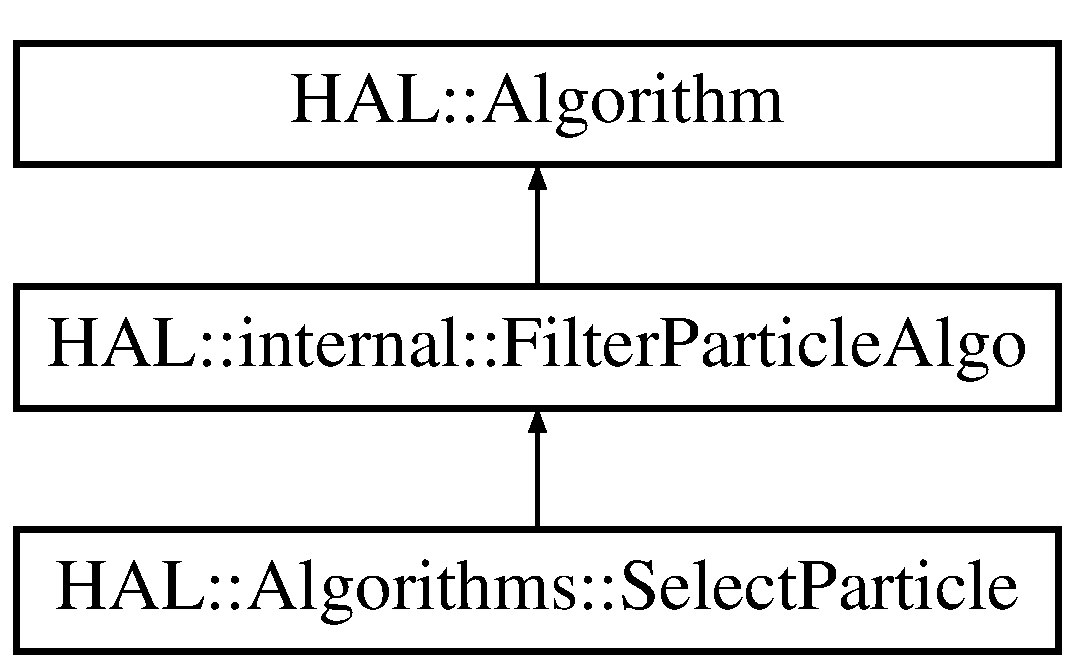
\includegraphics[height=3.000000cm]{class_h_a_l_1_1_algorithms_1_1_select_particle}
\end{center}
\end{figure}
\subsection*{Public Member Functions}
\begin{DoxyCompactItemize}
\item 
\hyperlink{class_h_a_l_1_1_algorithms_1_1_select_particle_a54e0c4f2c30c5dadd99c92c2d74ed37c}{Select\+Particle} (T\+String name, T\+String title, T\+String input, T\+String property, T\+String logic, double value)
\begin{DoxyCompactList}\small\item\em Constructor. \end{DoxyCompactList}\item 
\hyperlink{class_h_a_l_1_1_algorithms_1_1_select_particle_a66727ef056247051056804562276ff84}{Select\+Particle} (T\+String name, T\+String title, T\+String input, T\+String property, T\+String inclusion, double low, double high)
\begin{DoxyCompactList}\small\item\em Constructor. \end{DoxyCompactList}\item 
\hyperlink{class_h_a_l_1_1_algorithms_1_1_select_particle_a0eaa8644614c2d1d2db3b79e5c189a9a}{Select\+Particle} (T\+String name, T\+String title, T\+String input, T\+String property, int length,...)
\begin{DoxyCompactList}\small\item\em Constructor. \end{DoxyCompactList}\end{DoxyCompactItemize}
\subsection*{Protected Member Functions}
\begin{DoxyCompactItemize}
\item 
\hypertarget{class_h_a_l_1_1_algorithms_1_1_select_particle_af19a208179b5c2da43bdd010ec7355cd}{virtual bool {\bfseries Filter\+Predicate} (\hyperlink{class_h_a_l_1_1_generic_particle}{H\+A\+L\+::\+Particle\+Ptr})}\label{class_h_a_l_1_1_algorithms_1_1_select_particle_af19a208179b5c2da43bdd010ec7355cd}

\end{DoxyCompactItemize}


\subsection{Detailed Description}
Generic algorithm class that selects particles with specified properties. 

This algorithm selects particles relative to a specified property. This algorithm can select particles by a simple relationship, windowed between two values, or a list of values of a specified property. How the selection occurs is determined by the constructor used to initialize the algorithm. The list of available properties and relationships are given below. Properties and relationships are input as strings to the constructor of this algorithm. The particle from this algorithm is stored in a \hyperlink{class_h_a_l_1_1_generic_data}{Generic\+Data} object in the User\+Data under the algorithm's name.~\newline
~\newline
{\itshape Available Properties\+:} \begin{TabularC}{10}
\hline
\rowcolor{lightgray}\PBS\centering {\bf $ p_T $ }&\PBS\centering {\bf $ E_T $ }&\PBS\centering {\bf Mass }&\PBS\centering {\bf Energy }&\PBS\centering {\bf $ \left|\overrightarrow{p}\right| $ }&\PBS\centering {\bf $ \eta $ }&\PBS\centering {\bf $ \phi $ }&\PBS\centering {\bf I\+D }&\PBS\centering {\bf Charge }&\PBS\centering {\bf Custom Attribute  }\\\cline{1-10}
\PBS\centering p\+T &\PBS\centering e\+T &\PBS\centering m &\PBS\centering e &\PBS\centering p3 &\PBS\centering eta &\PBS\centering phi &\PBS\centering id &\PBS\centering charge &\PBS\centering $<$attribute$>$ \\\cline{1-10}
\end{TabularC}
{\itshape Available Logical Relationships\+:} \begin{TabularC}{6}
\hline
\rowcolor{lightgray}\PBS\centering {\bf Equal }&\PBS\centering {\bf Not Equal }&\PBS\centering {\bf Greater Than }&\PBS\centering {\bf Greater Than or Equal To }&\PBS\centering {\bf Less Than }&\PBS\centering {\bf Less Than or Equal To  }\\\cline{1-6}
\PBS\centering == &\PBS\centering != &\PBS\centering $>$ &\PBS\centering $>$= &\PBS\centering $<$ &\PBS\centering $<$= \\\cline{1-6}
\end{TabularC}
{\itshape Note\+:} = may also be used in place of ==.~\newline
~\newline
{\bfseries Examples\+:}~\newline
In your analysis file, do the following to select the muons with $ p_T $ greater than or equal to 50\+Ge\+V\+:


\begin{DoxyCode}
\hyperlink{class_h_a_l_1_1_analysis}{HAL::Analysis} a(\textcolor{stringliteral}{"sample analysis"}, \textcolor{stringliteral}{""}, \textcolor{stringliteral}{"truth"});

a.AddAlgo(\textcolor{keyword}{new} \hyperlink{class_h_a_l_1_1_algorithms_1_1_import_particle}{HAL::Algorithms::ImportParticle}(\textcolor{stringliteral}{"muons"}, \textcolor{stringliteral}{"import basic muons"})
      );

\textcolor{comment}{//...}

a.AddAlgo(\textcolor{keyword}{new} \hyperlink{class_h_a_l_1_1_algorithms_1_1_select_particle}{HAL::Algorithms::SelectParticle}(\textcolor{stringliteral}{"muons pT"}, \textcolor{stringliteral}{"select muons with
       pt >= 50GeV"}, 
                                              \textcolor{stringliteral}{"muons"},
                                              \textcolor{stringliteral}{"pt"}, \textcolor{stringliteral}{">="}, 50000));
\end{DoxyCode}
 To select the muons within an $ \eta $ value between -\/2.\+0 and 2.\+0 but not between -\/0.\+5 and 0.\+5\+:


\begin{DoxyCode}
\hyperlink{class_h_a_l_1_1_analysis}{HAL::Analysis} a(\textcolor{stringliteral}{"sample analysis"}, \textcolor{stringliteral}{""}, \textcolor{stringliteral}{"truth"});

a.AddAlgo(\textcolor{keyword}{new} \hyperlink{class_h_a_l_1_1_algorithms_1_1_import_particle}{HAL::Algorithms::ImportParticle}(\textcolor{stringliteral}{"muons"}, \textcolor{stringliteral}{"import basic muons"})
      );

\textcolor{comment}{//...}

a.AddAlgo(\textcolor{keyword}{new} \hyperlink{class_h_a_l_1_1_algorithms_1_1_select_particle}{HAL::Algorithms::SelectParticle}(\textcolor{stringliteral}{"muons |eta| <= 2.0"}, \textcolor{stringliteral}{"select
       muons with |eta| <= 2.0"}, 
                                              \textcolor{stringliteral}{"muons"},
                                              \textcolor{stringliteral}{"eta"}, \textcolor{stringliteral}{"inclusive"}, -2.0, 2.0));
a.AddAlgo(\textcolor{keyword}{new} \hyperlink{class_h_a_l_1_1_algorithms_1_1_select_particle}{HAL::Algorithms::SelectParticle}(\textcolor{stringliteral}{"muons eta"}, \textcolor{stringliteral}{"select muons
       with |eta| >= 0.5"}, 
                                              \textcolor{stringliteral}{"muons |eta| <= 2.0"},
                                              \textcolor{stringliteral}{"eta"}, \textcolor{stringliteral}{"exclusive"}, -0.5, 0.5));
\end{DoxyCode}
 To select the Monte Carlo particles with P\+D\+G I\+D's of neutrinos\+:


\begin{DoxyCode}
\hyperlink{class_h_a_l_1_1_analysis}{HAL::Analysis} a(\textcolor{stringliteral}{"sample analysis"}, \textcolor{stringliteral}{""}, \textcolor{stringliteral}{"truth"});

a.AddAlgo(\textcolor{keyword}{new} \hyperlink{class_h_a_l_1_1_algorithms_1_1_import_particle}{HAL::Algorithms::ImportParticle}(\textcolor{stringliteral}{"mc"}, \textcolor{stringliteral}{"import basic Monte
       Carlo particles"}));

\textcolor{comment}{//...}

a.AddAlgo(\textcolor{keyword}{new} \hyperlink{class_h_a_l_1_1_algorithms_1_1_select_particle}{HAL::Algorithms::SelectParticle}(\textcolor{stringliteral}{"mc\_neutrinos"}, \textcolor{stringliteral}{"filter on mc
       id to get neutrinos"}, 
                                              \textcolor{stringliteral}{"mc"},
                                              \textcolor{stringliteral}{"id"}, 6,
                                              -16, -14, -12, 12, 14, 16));
\end{DoxyCode}
 

\subsection{Constructor \& Destructor Documentation}
\hypertarget{class_h_a_l_1_1_algorithms_1_1_select_particle_a54e0c4f2c30c5dadd99c92c2d74ed37c}{\index{H\+A\+L\+::\+Algorithms\+::\+Select\+Particle@{H\+A\+L\+::\+Algorithms\+::\+Select\+Particle}!Select\+Particle@{Select\+Particle}}
\index{Select\+Particle@{Select\+Particle}!H\+A\+L\+::\+Algorithms\+::\+Select\+Particle@{H\+A\+L\+::\+Algorithms\+::\+Select\+Particle}}
\subsubsection[{Select\+Particle}]{\setlength{\rightskip}{0pt plus 5cm}H\+A\+L\+::\+Algorithms\+::\+Select\+Particle\+::\+Select\+Particle (
\begin{DoxyParamCaption}
\item[{T\+String}]{name, }
\item[{T\+String}]{title, }
\item[{T\+String}]{input, }
\item[{T\+String}]{property, }
\item[{T\+String}]{logic, }
\item[{double}]{value}
\end{DoxyParamCaption}
)}}\label{class_h_a_l_1_1_algorithms_1_1_select_particle_a54e0c4f2c30c5dadd99c92c2d74ed37c}


Constructor. 

Initializes the algorithm for simple relational selection 
\begin{DoxyParams}[1]{Parameters}
\mbox{\tt in}  & {\em name} & Name of the algorithm. This can be used as the input to other algorithms. \\
\hline
\mbox{\tt in}  & {\em title} & Description of the algorithm. Can be an empty string. \\
\hline
\mbox{\tt in}  & {\em input} & Name of algorithm to select from. \\
\hline
\mbox{\tt in}  & {\em property} & Property by which to select particles. \\
\hline
\mbox{\tt in}  & {\em logic} & How to select the particles. \\
\hline
\mbox{\tt in}  & {\em value} & Value of property. \\
\hline
\end{DoxyParams}
\begin{DoxySeeAlso}{See also}
\hyperlink{class_h_a_l_1_1_algorithms_1_1_import_particle}{Import\+Particle}, \hyperlink{class_h_a_l_1_1_algorithms_1_1_particle_rank_selection}{Particle\+Rank\+Selection} 
\end{DoxySeeAlso}
\hypertarget{class_h_a_l_1_1_algorithms_1_1_select_particle_a66727ef056247051056804562276ff84}{\index{H\+A\+L\+::\+Algorithms\+::\+Select\+Particle@{H\+A\+L\+::\+Algorithms\+::\+Select\+Particle}!Select\+Particle@{Select\+Particle}}
\index{Select\+Particle@{Select\+Particle}!H\+A\+L\+::\+Algorithms\+::\+Select\+Particle@{H\+A\+L\+::\+Algorithms\+::\+Select\+Particle}}
\subsubsection[{Select\+Particle}]{\setlength{\rightskip}{0pt plus 5cm}H\+A\+L\+::\+Algorithms\+::\+Select\+Particle\+::\+Select\+Particle (
\begin{DoxyParamCaption}
\item[{T\+String}]{name, }
\item[{T\+String}]{title, }
\item[{T\+String}]{input, }
\item[{T\+String}]{property, }
\item[{T\+String}]{inclusion, }
\item[{double}]{low, }
\item[{double}]{high}
\end{DoxyParamCaption}
)}}\label{class_h_a_l_1_1_algorithms_1_1_select_particle_a66727ef056247051056804562276ff84}


Constructor. 

Initializes the algorithm for a window selection 
\begin{DoxyParams}[1]{Parameters}
\mbox{\tt in}  & {\em name} & Name of the algorithm. This can be used as the input to other algorithms. \\
\hline
\mbox{\tt in}  & {\em title} & Description of the algorithm. Can be an empty string. \\
\hline
\mbox{\tt in}  & {\em input} & Name of algorithm to select from. \\
\hline
\mbox{\tt in}  & {\em property} & Property by which to select particles. \\
\hline
\mbox{\tt in}  & {\em inclusion} & How to select the particles. Either inclusive (or in) or exclusive (or out). \\
\hline
\mbox{\tt in}  & {\em low} & Lower value of property. \\
\hline
\mbox{\tt in}  & {\em high} & Higher value of property. \\
\hline
\end{DoxyParams}
\begin{DoxySeeAlso}{See also}
\hyperlink{class_h_a_l_1_1_algorithms_1_1_import_particle}{Import\+Particle}, \hyperlink{class_h_a_l_1_1_algorithms_1_1_particle_rank_selection}{Particle\+Rank\+Selection} 
\end{DoxySeeAlso}
\hypertarget{class_h_a_l_1_1_algorithms_1_1_select_particle_a0eaa8644614c2d1d2db3b79e5c189a9a}{\index{H\+A\+L\+::\+Algorithms\+::\+Select\+Particle@{H\+A\+L\+::\+Algorithms\+::\+Select\+Particle}!Select\+Particle@{Select\+Particle}}
\index{Select\+Particle@{Select\+Particle}!H\+A\+L\+::\+Algorithms\+::\+Select\+Particle@{H\+A\+L\+::\+Algorithms\+::\+Select\+Particle}}
\subsubsection[{Select\+Particle}]{\setlength{\rightskip}{0pt plus 5cm}H\+A\+L\+::\+Algorithms\+::\+Select\+Particle\+::\+Select\+Particle (
\begin{DoxyParamCaption}
\item[{T\+String}]{name, }
\item[{T\+String}]{title, }
\item[{T\+String}]{input, }
\item[{T\+String}]{property, }
\item[{int}]{length, }
\item[{}]{...}
\end{DoxyParamCaption}
)}}\label{class_h_a_l_1_1_algorithms_1_1_select_particle_a0eaa8644614c2d1d2db3b79e5c189a9a}


Constructor. 

Initializes the algorithm for specific values selection 
\begin{DoxyParams}[1]{Parameters}
\mbox{\tt in}  & {\em name} & Name of the algorithm. This can be used as the input to other algorithms. \\
\hline
\mbox{\tt in}  & {\em title} & Description of the algorithm. Can be an empty string. \\
\hline
\mbox{\tt in}  & {\em input} & Name of algorithm to select from. \\
\hline
\mbox{\tt in}  & {\em property} & Property by which to select particles. \\
\hline
\mbox{\tt in}  & {\em length} & Number of values to compare against. \\
\hline
\mbox{\tt in}  & {\em ...} & Comma separated list of values. If property is id use integer values, otherwise use decimal values. \\
\hline
\end{DoxyParams}
\begin{DoxySeeAlso}{See also}
\hyperlink{class_h_a_l_1_1_algorithms_1_1_import_particle}{Import\+Particle}, \hyperlink{class_h_a_l_1_1_algorithms_1_1_particle_rank_selection}{Particle\+Rank\+Selection} 
\end{DoxySeeAlso}


The documentation for this class was generated from the following file\+:\begin{DoxyCompactItemize}
\item 
/\+Users/jhetherly/src/root\+\_\+\+H\+A\+L/include/\+H\+A\+L/\hyperlink{_algorithms_8h}{Algorithms.\+h}\end{DoxyCompactItemize}

\hypertarget{class_h_a_l_1_1_algorithms_1_1_select_ref_particle}{\section{H\-A\-L\-:\-:Algorithms\-:\-:Select\-Ref\-Particle Class Reference}
\label{class_h_a_l_1_1_algorithms_1_1_select_ref_particle}\index{H\-A\-L\-::\-Algorithms\-::\-Select\-Ref\-Particle@{H\-A\-L\-::\-Algorithms\-::\-Select\-Ref\-Particle}}
}


Generic algorithm class that selects particles with respect to a reference particle.  




{\ttfamily \#include $<$Algorithms.\-h$>$}

Inheritance diagram for H\-A\-L\-:\-:Algorithms\-:\-:Select\-Ref\-Particle\-:\begin{figure}[H]
\begin{center}
\leavevmode
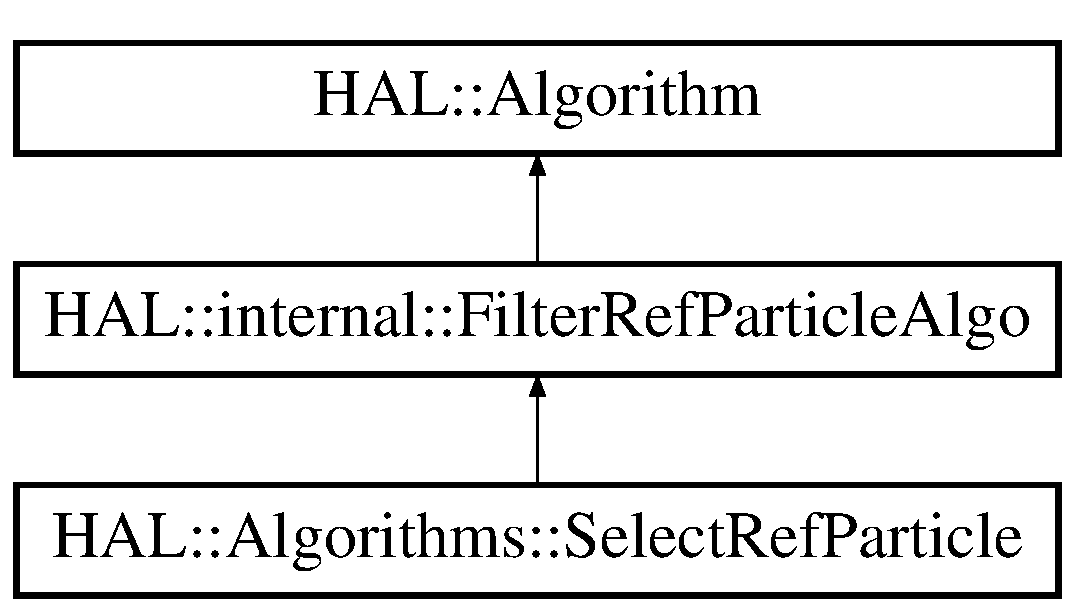
\includegraphics[height=3.000000cm]{class_h_a_l_1_1_algorithms_1_1_select_ref_particle}
\end{center}
\end{figure}
\subsection*{Public Member Functions}
\begin{DoxyCompactItemize}
\item 
\hyperlink{class_h_a_l_1_1_algorithms_1_1_select_ref_particle_af0c5f5e66e54f7bc102e32148867892e}{Select\-Ref\-Particle} (T\-String name, T\-String title, T\-String reference, T\-String input, double value, T\-String property=\char`\"{}dr\char`\"{}, T\-String inclusion=\char`\"{}inclusive\char`\"{})
\begin{DoxyCompactList}\small\item\em Constructor. \end{DoxyCompactList}\item 
\hyperlink{class_h_a_l_1_1_algorithms_1_1_select_ref_particle_a68f9c3c857223c9a84b73e1569cdecaf}{Select\-Ref\-Particle} (T\-String name, T\-String title, T\-String reference, T\-String input, double low, double high, T\-String property=\char`\"{}dr\char`\"{}, T\-String inclusion=\char`\"{}inclusive\char`\"{})
\begin{DoxyCompactList}\small\item\em Constructor. \end{DoxyCompactList}\end{DoxyCompactItemize}
\subsection*{Protected Member Functions}
\begin{DoxyCompactItemize}
\item 
\hypertarget{class_h_a_l_1_1_algorithms_1_1_select_ref_particle_a04fa4b96a01e34c5ee0bb8782eb51b00}{virtual bool {\bfseries Filter\-Predicate} (\hyperlink{class_h_a_l_1_1_generic_particle}{H\-A\-L\-::\-Particle\-Ptr}, \hyperlink{class_h_a_l_1_1_generic_particle}{H\-A\-L\-::\-Particle\-Ptr})}\label{class_h_a_l_1_1_algorithms_1_1_select_ref_particle_a04fa4b96a01e34c5ee0bb8782eb51b00}

\end{DoxyCompactItemize}
\subsection*{Additional Inherited Members}


\subsection{Detailed Description}
Generic algorithm class that selects particles with respect to a reference particle. 

This algorithm selects particles relative to a reference particle. This algorithm makes sure to not compare the same particle to itself. An inclusive, exclusive, or windowed selection is determined by the constructor used to initialize the algorithm. The properties are listed below. The particle from this algorithm is stored in a \hyperlink{class_h_a_l_1_1_generic_data}{Generic\-Data} object in the User\-Data under the algorithm's name.\par
\par
 {\itshape Available Properties\-:} \begin{TabularC}{2}
\hline
\rowcolor{lightgray}\PBS\centering {\bf $ \Delta R $ }&\PBS\centering {\bf $ \Delta\phi $ }\\\cline{1-2}
\PBS\centering dr &\PBS\centering dphi \\\cline{1-2}
\end{TabularC}
{\bfseries Example\-:}\par
 In your analysis file, do the following to select the jets within a $ \Delta R $ of 0.\-4 from the highest $ p_T $ jet\-:


\begin{DoxyCode}
\hyperlink{class_h_a_l_1_1_analysis}{HAL::Analysis} a(\textcolor{stringliteral}{"sample analysis"}, \textcolor{stringliteral}{""}, \textcolor{stringliteral}{"truth"});

a.AddAlgo(\textcolor{keyword}{new} \hyperlink{class_h_a_l_1_1_algorithms_1_1_import_particle}{HAL::Algorithms::ImportParticle}(\textcolor{stringliteral}{"jets"}, \textcolor{stringliteral}{"import basic jets"}));

\textcolor{comment}{//...}

a.AddAlgo(\textcolor{keyword}{new} \hyperlink{class_h_a_l_1_1_algorithms_1_1_particle_rank_selection}{HAL::Algorithms::ParticleRankSelection}(\textcolor{stringliteral}{"leading pt jet"}
      , \textcolor{stringliteral}{"find highest pt jet"}, 
                                                     \textcolor{stringliteral}{"jets"},
                                                     1, \textcolor{stringliteral}{"pt"}));

a.AddAlgo(\textcolor{keyword}{new} \hyperlink{class_h_a_l_1_1_algorithms_1_1_select_ref_particle}{HAL::Algorithms::SelectRefParticle}(\textcolor{stringliteral}{"jets close"}, \textcolor{stringliteral}{"filter on
       jets within deltaR of di-jet"}, 
                                                 \textcolor{stringliteral}{"leading pt jet"}, \textcolor{stringliteral}{"jets"},
                                                 0.4, \textcolor{stringliteral}{"dr"}));
\end{DoxyCode}
 

\subsection{Constructor \& Destructor Documentation}
\hypertarget{class_h_a_l_1_1_algorithms_1_1_select_ref_particle_af0c5f5e66e54f7bc102e32148867892e}{\index{H\-A\-L\-::\-Algorithms\-::\-Select\-Ref\-Particle@{H\-A\-L\-::\-Algorithms\-::\-Select\-Ref\-Particle}!Select\-Ref\-Particle@{Select\-Ref\-Particle}}
\index{Select\-Ref\-Particle@{Select\-Ref\-Particle}!HAL::Algorithms::SelectRefParticle@{H\-A\-L\-::\-Algorithms\-::\-Select\-Ref\-Particle}}
\subsubsection[{Select\-Ref\-Particle}]{\setlength{\rightskip}{0pt plus 5cm}H\-A\-L\-::\-Algorithms\-::\-Select\-Ref\-Particle\-::\-Select\-Ref\-Particle (
\begin{DoxyParamCaption}
\item[{T\-String}]{name, }
\item[{T\-String}]{title, }
\item[{T\-String}]{reference, }
\item[{T\-String}]{input, }
\item[{double}]{value, }
\item[{T\-String}]{property = {\ttfamily \char`\"{}dr\char`\"{}}, }
\item[{T\-String}]{inclusion = {\ttfamily \char`\"{}inclusive\char`\"{}}}
\end{DoxyParamCaption}
)}}\label{class_h_a_l_1_1_algorithms_1_1_select_ref_particle_af0c5f5e66e54f7bc102e32148867892e}


Constructor. 

Initializes the algorithm for a simple selection 
\begin{DoxyParams}[1]{Parameters}
\mbox{\tt in}  & {\em name} & Name of the algorithm. This can be used as the input to other algorithms. \\
\hline
\mbox{\tt in}  & {\em title} & Description of the algorithm. Can be an empty string. \\
\hline
\mbox{\tt in}  & {\em reference} & Name of algorithm the reference particle. \\
\hline
\mbox{\tt in}  & {\em input} & Name of algorithm to select from. \\
\hline
\mbox{\tt in}  & {\em value} & Value of property \\
\hline
\mbox{\tt in}  & {\em property} & Property by which to select particles. \\
\hline
\mbox{\tt in}  & {\em inclusion} & How to select the particles. Either inclusive (or in) or exclusive (or out). \\
\hline
\end{DoxyParams}
\begin{DoxySeeAlso}{See Also}
\hyperlink{class_h_a_l_1_1_algorithms_1_1_import_particle}{Import\-Particle}, \hyperlink{class_h_a_l_1_1_algorithms_1_1_particle_rank_selection}{Particle\-Rank\-Selection} 
\end{DoxySeeAlso}
\hypertarget{class_h_a_l_1_1_algorithms_1_1_select_ref_particle_a68f9c3c857223c9a84b73e1569cdecaf}{\index{H\-A\-L\-::\-Algorithms\-::\-Select\-Ref\-Particle@{H\-A\-L\-::\-Algorithms\-::\-Select\-Ref\-Particle}!Select\-Ref\-Particle@{Select\-Ref\-Particle}}
\index{Select\-Ref\-Particle@{Select\-Ref\-Particle}!HAL::Algorithms::SelectRefParticle@{H\-A\-L\-::\-Algorithms\-::\-Select\-Ref\-Particle}}
\subsubsection[{Select\-Ref\-Particle}]{\setlength{\rightskip}{0pt plus 5cm}H\-A\-L\-::\-Algorithms\-::\-Select\-Ref\-Particle\-::\-Select\-Ref\-Particle (
\begin{DoxyParamCaption}
\item[{T\-String}]{name, }
\item[{T\-String}]{title, }
\item[{T\-String}]{reference, }
\item[{T\-String}]{input, }
\item[{double}]{low, }
\item[{double}]{high, }
\item[{T\-String}]{property = {\ttfamily \char`\"{}dr\char`\"{}}, }
\item[{T\-String}]{inclusion = {\ttfamily \char`\"{}inclusive\char`\"{}}}
\end{DoxyParamCaption}
)}}\label{class_h_a_l_1_1_algorithms_1_1_select_ref_particle_a68f9c3c857223c9a84b73e1569cdecaf}


Constructor. 

Initializes the algorithm for a window selection 
\begin{DoxyParams}[1]{Parameters}
\mbox{\tt in}  & {\em name} & Name of the algorithm. This can be used as the input to other algorithms. \\
\hline
\mbox{\tt in}  & {\em title} & Description of the algorithm. Can be an empty string. \\
\hline
\mbox{\tt in}  & {\em reference} & Name of algorithm the reference particle. \\
\hline
\mbox{\tt in}  & {\em input} & Name of algorithm to select from. \\
\hline
\mbox{\tt in}  & {\em low} & Lower value of property. \\
\hline
\mbox{\tt in}  & {\em high} & Higher value of property. \\
\hline
\mbox{\tt in}  & {\em property} & Property by which to select particles. \\
\hline
\mbox{\tt in}  & {\em inclusion} & How to select the particles. Either inclusive (or in) or exclusive (or out). \\
\hline
\end{DoxyParams}
\begin{DoxySeeAlso}{See Also}
\hyperlink{class_h_a_l_1_1_algorithms_1_1_import_particle}{Import\-Particle}, \hyperlink{class_h_a_l_1_1_algorithms_1_1_particle_rank_selection}{Particle\-Rank\-Selection} 
\end{DoxySeeAlso}


The documentation for this class was generated from the following file\-:\begin{DoxyCompactItemize}
\item 
/\-Users/jhetherly/src/root\-\_\-\-H\-A\-L/include/\-H\-A\-L/\hyperlink{_algorithms_8h}{Algorithms.\-h}\end{DoxyCompactItemize}

\hypertarget{class_h_a_l_1_1_algorithms_1_1_store_particle}{\section{H\+A\+L\+:\+:Algorithms\+:\+:Store\+Particle Class Reference}
\label{class_h_a_l_1_1_algorithms_1_1_store_particle}\index{H\+A\+L\+::\+Algorithms\+::\+Store\+Particle@{H\+A\+L\+::\+Algorithms\+::\+Store\+Particle}}
}


\hyperlink{class_h_a_l_1_1_algorithm}{Algorithm} that stores the properties of particles to a T\+Tree.  




{\ttfamily \#include $<$Store\+Particle.\+h$>$}

Inheritance diagram for H\+A\+L\+:\+:Algorithms\+:\+:Store\+Particle\+:\begin{figure}[H]
\begin{center}
\leavevmode
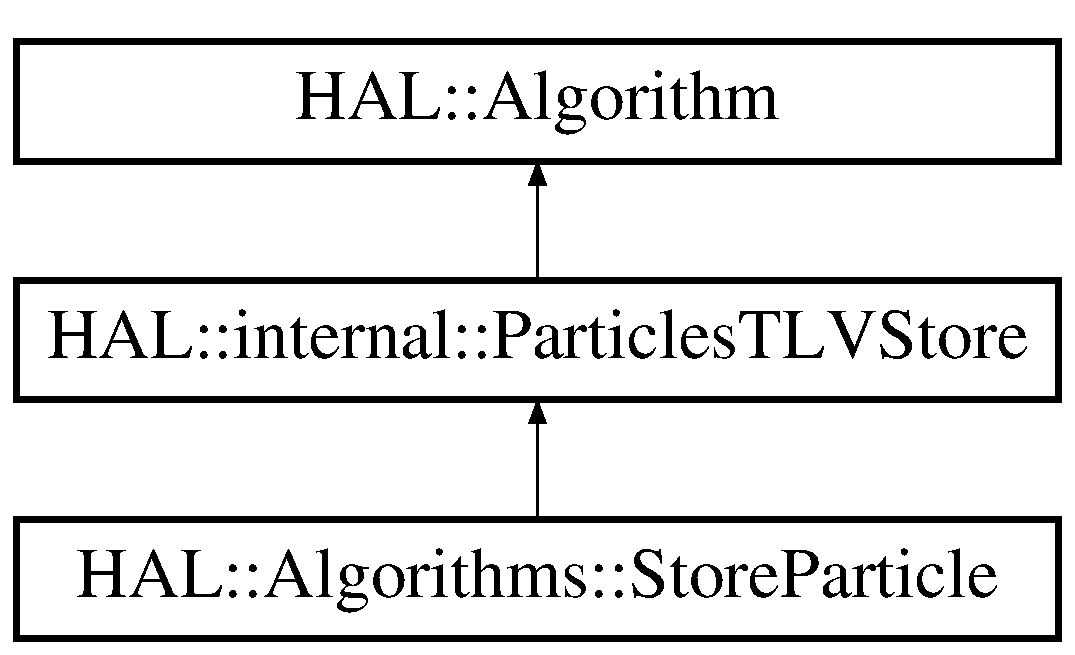
\includegraphics[height=3.000000cm]{class_h_a_l_1_1_algorithms_1_1_store_particle}
\end{center}
\end{figure}
\subsection*{Public Member Functions}
\begin{DoxyCompactItemize}
\item 
\hyperlink{class_h_a_l_1_1_algorithms_1_1_store_particle_a160a46b43875d8968e865fc2335380f3}{Store\+Particle} (T\+String name, T\+String title, T\+String input, T\+String property, T\+String bname, T\+String tname=\char`\"{}\char`\"{})
\begin{DoxyCompactList}\small\item\em Constructor. \end{DoxyCompactList}\end{DoxyCompactItemize}
\subsection*{Protected Member Functions}
\begin{DoxyCompactItemize}
\item 
virtual void \hyperlink{class_h_a_l_1_1_algorithms_1_1_store_particle_af2e287e256a0d7803c68a62bbb254302}{Init} (Option\+\_\+t $\ast$)
\begin{DoxyCompactList}\small\item\em Hook into the T\+Selector\+::\+Init method. \end{DoxyCompactList}\item 
\hypertarget{class_h_a_l_1_1_algorithms_1_1_store_particle_acf9039e1285e48324c378295cf4cea3b}{virtual void {\bfseries Store\+Value} (\hyperlink{class_h_a_l_1_1_analysis_tree_writer}{H\+A\+L\+::\+Analysis\+Tree\+Writer} $\ast$, long long, \hyperlink{class_h_a_l_1_1_generic_particle}{H\+A\+L\+::\+Particle\+Ptr})}\label{class_h_a_l_1_1_algorithms_1_1_store_particle_acf9039e1285e48324c378295cf4cea3b}

\end{DoxyCompactItemize}


\subsection{Detailed Description}
\hyperlink{class_h_a_l_1_1_algorithm}{Algorithm} that stores the properties of particles to a T\+Tree. 

This algorithm stores particles or specific parts of particles in a specified T\+Tree. The user needs only supply a branch name, property, and a tree name (optional). If the \char`\"{}all\char`\"{} property is given, the branch name given will act as the base for all other properties, i.\+e. if branch name is \char`\"{}jets\char`\"{}, the branches written will be \char`\"{}jets\+\_\+pt\char`\"{}, \char`\"{}jets\+\_\+eta\char`\"{}, etc. {\itshape Available Properties\+:} \begin{TabularC}{11}
\hline
\rowcolor{lightgray}\PBS\centering {\bf $ p_T $ }&\PBS\centering {\bf $ E_T $ }&\PBS\centering {\bf Mass }&\PBS\centering {\bf Energy }&\PBS\centering {\bf $ \left|\overrightarrow{p}\right| $ }&\PBS\centering {\bf $ \eta $ }&\PBS\centering {\bf $ \phi $ }&\PBS\centering {\bf I\+D }&\PBS\centering {\bf Charge }&\PBS\centering {\bf Full Particle }&\PBS\centering {\bf All Attributes  }\\\cline{1-11}
\PBS\centering p\+T &\PBS\centering e\+T &\PBS\centering m &\PBS\centering e &\PBS\centering p3 &\PBS\centering eta &\PBS\centering phi &\PBS\centering id &\PBS\centering charge &\PBS\centering all &\PBS\centering attributes \\\cline{1-11}
\end{TabularC}
{\bfseries Example\+:}~\newline
In your analysis file, do the following to store jet particles\+:


\begin{DoxyCode}
\hyperlink{class_h_a_l_1_1_analysis}{HAL::Analysis} a(\textcolor{stringliteral}{"sample analysis"}, \textcolor{stringliteral}{""}, \textcolor{stringliteral}{"truth"});

a.AddAlgo(\textcolor{keyword}{new} \hyperlink{class_h_a_l_1_1_algorithms_1_1_import_particle}{HAL::Algorithms::ImportParticle}(\textcolor{stringliteral}{"basic jets"}, \textcolor{stringliteral}{"import basic
       jet objects"}));

a.AddAlgo(\textcolor{keyword}{new} \hyperlink{class_h_a_l_1_1_algorithms_1_1_store_particle}{HAL::Algorithms::StoreParticle}(\textcolor{stringliteral}{"store jets"}, \textcolor{stringliteral}{"store jets"}, 
                                             \textcolor{stringliteral}{"basic jets"}, \textcolor{stringliteral}{"all"}, \textcolor{stringliteral}{"jets"}));
\end{DoxyCode}
 

\subsection{Constructor \& Destructor Documentation}
\hypertarget{class_h_a_l_1_1_algorithms_1_1_store_particle_a160a46b43875d8968e865fc2335380f3}{\index{H\+A\+L\+::\+Algorithms\+::\+Store\+Particle@{H\+A\+L\+::\+Algorithms\+::\+Store\+Particle}!Store\+Particle@{Store\+Particle}}
\index{Store\+Particle@{Store\+Particle}!H\+A\+L\+::\+Algorithms\+::\+Store\+Particle@{H\+A\+L\+::\+Algorithms\+::\+Store\+Particle}}
\subsubsection[{Store\+Particle}]{\setlength{\rightskip}{0pt plus 5cm}H\+A\+L\+::\+Algorithms\+::\+Store\+Particle\+::\+Store\+Particle (
\begin{DoxyParamCaption}
\item[{T\+String}]{name, }
\item[{T\+String}]{title, }
\item[{T\+String}]{input, }
\item[{T\+String}]{property, }
\item[{T\+String}]{bname, }
\item[{T\+String}]{tname = {\ttfamily \char`\"{}\char`\"{}}}
\end{DoxyParamCaption}
)}}\label{class_h_a_l_1_1_algorithms_1_1_store_particle_a160a46b43875d8968e865fc2335380f3}


Constructor. 

Initializes the algorithm. 
\begin{DoxyParams}[1]{Parameters}
\mbox{\tt in}  & {\em name} & Name of the algorithm. This can be used as the input to other algorithms. \\
\hline
\mbox{\tt in}  & {\em title} & Description of the algorithm. Can be an empty string. \\
\hline
\mbox{\tt in}  & {\em input} & Name of algorithm to store. \\
\hline
\mbox{\tt in}  & {\em property} & Property to store. \\
\hline
\mbox{\tt in}  & {\em bname} & Branch to store as. \\
\hline
\mbox{\tt in}  & {\em tname} & Tree to store in. \\
\hline
\end{DoxyParams}


\subsection{Member Function Documentation}
\hypertarget{class_h_a_l_1_1_algorithms_1_1_store_particle_af2e287e256a0d7803c68a62bbb254302}{\index{H\+A\+L\+::\+Algorithms\+::\+Store\+Particle@{H\+A\+L\+::\+Algorithms\+::\+Store\+Particle}!Init@{Init}}
\index{Init@{Init}!H\+A\+L\+::\+Algorithms\+::\+Store\+Particle@{H\+A\+L\+::\+Algorithms\+::\+Store\+Particle}}
\subsubsection[{Init}]{\setlength{\rightskip}{0pt plus 5cm}virtual void H\+A\+L\+::\+Algorithms\+::\+Store\+Particle\+::\+Init (
\begin{DoxyParamCaption}
\item[{Option\+\_\+t $\ast$}]{}
\end{DoxyParamCaption}
)\hspace{0.3cm}{\ttfamily [protected]}, {\ttfamily [virtual]}}}\label{class_h_a_l_1_1_algorithms_1_1_store_particle_af2e287e256a0d7803c68a62bbb254302}


Hook into the T\+Selector\+::\+Init method. 

This method allows the algorithm operate at the 'Init' stage of processing a T\+Tree. This method is called when a new T\+Tree is being prepared for processing. 
\begin{DoxyParams}[1]{Parameters}
\mbox{\tt in}  & {\em option} & Option string passed to all algorithms from the Analysis\+::\+Process call \\
\hline
\end{DoxyParams}


Reimplemented from \hyperlink{class_h_a_l_1_1_algorithm_abe2da2ce6a2d3ccfb492d8afd1d07331}{H\+A\+L\+::\+Algorithm}.



The documentation for this class was generated from the following file\+:\begin{DoxyCompactItemize}
\item 
/\+Users/jhetherly/src/\+H\+A\+L-\/\+R\+O\+O\+T/include/\+H\+A\+L/\+Algorithms/\hyperlink{_store_particle_8h}{Store\+Particle.\+h}\end{DoxyCompactItemize}

\hypertarget{class_h_a_l_1_1_algorithms_1_1_vec_add_reco}{\section{H\+A\+L\+:\+:Algorithms\+:\+:Vec\+Add\+Reco Class Reference}
\label{class_h_a_l_1_1_algorithms_1_1_vec_add_reco}\index{H\+A\+L\+::\+Algorithms\+::\+Vec\+Add\+Reco@{H\+A\+L\+::\+Algorithms\+::\+Vec\+Add\+Reco}}
}


Generic algorithm class that combines tuples of particles from any number of alogrithms.  




{\ttfamily \#include $<$Vec\+Add\+Reco.\+h$>$}

Inheritance diagram for H\+A\+L\+:\+:Algorithms\+:\+:Vec\+Add\+Reco\+:\begin{figure}[H]
\begin{center}
\leavevmode
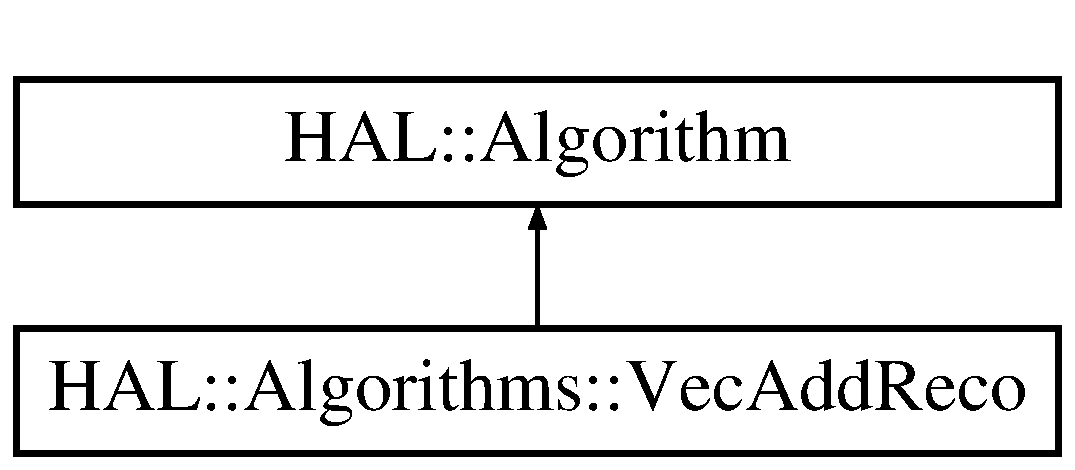
\includegraphics[height=2.000000cm]{class_h_a_l_1_1_algorithms_1_1_vec_add_reco}
\end{center}
\end{figure}
\subsection*{Public Member Functions}
\begin{DoxyCompactItemize}
\item 
\hyperlink{class_h_a_l_1_1_algorithms_1_1_vec_add_reco_a50faa627aa37f90ac35eccb3f24fb851}{Vec\+Add\+Reco} (T\+String name, T\+String title, long long length,...)
\begin{DoxyCompactList}\small\item\em Constructor. \end{DoxyCompactList}\end{DoxyCompactItemize}
\subsection*{Protected Member Functions}
\begin{DoxyCompactItemize}
\item 
\hypertarget{class_h_a_l_1_1_algorithms_1_1_vec_add_reco_a63f7458fec37ae553418b15a375dafa0}{virtual void {\bfseries Exec} (Option\+\_\+t $\ast$)}\label{class_h_a_l_1_1_algorithms_1_1_vec_add_reco_a63f7458fec37ae553418b15a375dafa0}

\item 
\hypertarget{class_h_a_l_1_1_algorithms_1_1_vec_add_reco_afcf9f83e8165c1cbd7a193ab8f9c8445}{virtual void {\bfseries Clear} (Option\+\_\+t $\ast$)}\label{class_h_a_l_1_1_algorithms_1_1_vec_add_reco_afcf9f83e8165c1cbd7a193ab8f9c8445}

\end{DoxyCompactItemize}
\subsection*{Additional Inherited Members}


\subsection{Detailed Description}
Generic algorithm class that combines tuples of particles from any number of alogrithms. 

This algorithm builds particles from the vector addition of other particles from an arbitrary number of other algorithms. Special care is taken to only add unique vectors (parents are also checked). Also, the tuples will be made up of as many particles as there are input algorithms (i.\+e. \char`\"{}length\char`\"{}). This algorithm may return no particles if no unique combination can be found. The particles from this algorithm are stored in a \hyperlink{class_h_a_l_1_1_generic_data}{Generic\+Data} object in the User\+Data under the algorithm's name.~\newline
~\newline
{\bfseries Example\+:}~\newline
In your analysis file, do the following for the vector addition of two muons\+:


\begin{DoxyCode}
\hyperlink{class_h_a_l_1_1_analysis}{HAL::Analysis} a(\textcolor{stringliteral}{"sample analysis"}, \textcolor{stringliteral}{""}, \textcolor{stringliteral}{"truth"});

a.AddAlgo(\textcolor{keyword}{new} \hyperlink{class_h_a_l_1_1_algorithms_1_1_import_particle}{HAL::Algorithms::ImportParticle}(\textcolor{stringliteral}{"muons"}, \textcolor{stringliteral}{"import basic muons"})
      );

\textcolor{comment}{//...}

a.AddAlgo(\textcolor{keyword}{new} \hyperlink{class_h_a_l_1_1_algorithms_1_1_vec_add_reco}{HAL::Algorithms::VecAddReco}(\textcolor{stringliteral}{"di-muons"}, \textcolor{stringliteral}{"combine muons pairwise"}, 
                                          2,
                                          \textcolor{stringliteral}{"muons"}, \textcolor{stringliteral}{"muons"}));
\end{DoxyCode}
 

\subsection{Constructor \& Destructor Documentation}
\hypertarget{class_h_a_l_1_1_algorithms_1_1_vec_add_reco_a50faa627aa37f90ac35eccb3f24fb851}{\index{H\+A\+L\+::\+Algorithms\+::\+Vec\+Add\+Reco@{H\+A\+L\+::\+Algorithms\+::\+Vec\+Add\+Reco}!Vec\+Add\+Reco@{Vec\+Add\+Reco}}
\index{Vec\+Add\+Reco@{Vec\+Add\+Reco}!H\+A\+L\+::\+Algorithms\+::\+Vec\+Add\+Reco@{H\+A\+L\+::\+Algorithms\+::\+Vec\+Add\+Reco}}
\subsubsection[{Vec\+Add\+Reco}]{\setlength{\rightskip}{0pt plus 5cm}H\+A\+L\+::\+Algorithms\+::\+Vec\+Add\+Reco\+::\+Vec\+Add\+Reco (
\begin{DoxyParamCaption}
\item[{T\+String}]{name, }
\item[{T\+String}]{title, }
\item[{long long}]{length, }
\item[{}]{...}
\end{DoxyParamCaption}
)}}\label{class_h_a_l_1_1_algorithms_1_1_vec_add_reco_a50faa627aa37f90ac35eccb3f24fb851}


Constructor. 

Initializes the algorithm 
\begin{DoxyParams}[1]{Parameters}
\mbox{\tt in}  & {\em name} & Name of the algorithm. This can be used as the input to other algorithms. \\
\hline
\mbox{\tt in}  & {\em title} & Description of the algorithm. Can be an empty string. \\
\hline
\mbox{\tt in}  & {\em length} & Number of algorithms to combine. \\
\hline
\mbox{\tt in}  & {\em ...} & Comma separated list of string literals representing the algorithms to combine. \\
\hline
\end{DoxyParams}
\begin{DoxySeeAlso}{See also}
\hyperlink{class_h_a_l_1_1_algorithms_1_1_import_particle}{Import\+Particle} 
\end{DoxySeeAlso}


The documentation for this class was generated from the following file\+:\begin{DoxyCompactItemize}
\item 
/\+Users/jhetherly/src/\+H\+A\+L-\/\+R\+O\+O\+T/include/\+H\+A\+L/\+Algorithms/\hyperlink{_vec_add_reco_8h}{Vec\+Add\+Reco.\+h}\end{DoxyCompactItemize}

\chapter{File Documentation}
\hypertarget{_attach_attribute_8h}{\section{/\+Users/jhetherly/src/\+H\+A\+L-\/\+R\+O\+O\+T/include/\+H\+A\+L/\+Algorithms/\+Attach\+Attribute.h File Reference}
\label{_attach_attribute_8h}\index{/\+Users/jhetherly/src/\+H\+A\+L-\/\+R\+O\+O\+T/include/\+H\+A\+L/\+Algorithms/\+Attach\+Attribute.\+h@{/\+Users/jhetherly/src/\+H\+A\+L-\/\+R\+O\+O\+T/include/\+H\+A\+L/\+Algorithms/\+Attach\+Attribute.\+h}}
}
{\ttfamily \#include $<$T\+Random3.\+h$>$}\\*
{\ttfamily \#include $<$T\+Named.\+h$>$}\\*
{\ttfamily \#include $<$T\+String.\+h$>$}\\*
{\ttfamily \#include $<$T\+Lorentz\+Vector.\+h$>$}\\*
{\ttfamily \#include $<$T\+Math.\+h$>$}\\*
{\ttfamily \#include $<$cstdarg$>$}\\*
{\ttfamily \#include $<$string$>$}\\*
{\ttfamily \#include $<$deque$>$}\\*
{\ttfamily \#include $<$vector$>$}\\*
{\ttfamily \#include $<$map$>$}\\*
{\ttfamily \#include $<$set$>$}\\*
{\ttfamily \#include $<$algorithm$>$}\\*
{\ttfamily \#include $<$iostream$>$}\\*
{\ttfamily \#include $<$H\+A\+L/\+Common.\+h$>$}\\*
{\ttfamily \#include $<$H\+A\+L/\+Exceptions.\+h$>$}\\*
{\ttfamily \#include $<$H\+A\+L/\+Analysis\+Utils.\+h$>$}\\*
{\ttfamily \#include $<$H\+A\+L/\+Algorithm.\+h$>$}\\*
{\ttfamily \#include $<$H\+A\+L/\+Cut\+Algorithm.\+h$>$}\\*
{\ttfamily \#include $<$H\+A\+L/\+Analysis\+Data.\+h$>$}\\*
{\ttfamily \#include $<$H\+A\+L/\+Analysis\+Tree\+Reader.\+h$>$}\\*
{\ttfamily \#include $<$H\+A\+L/\+Analysis\+Tree\+Writer.\+h$>$}\\*
{\ttfamily \#include $<$H\+A\+L/\+Generic\+Particle.\+h$>$}\\*
{\ttfamily \#include $<$H\+A\+L/\+Generic\+Data.\+h$>$}\\*
\subsection*{Classes}
\begin{DoxyCompactItemize}
\item 
class \hyperlink{class_h_a_l_1_1_algorithms_1_1_attach_attribute}{H\+A\+L\+::\+Algorithms\+::\+Attach\+Attribute}
\begin{DoxyCompactList}\small\item\em \hyperlink{class_h_a_l_1_1_algorithm}{Algorithm} that attaches a decimal value to an existing set of particles. \end{DoxyCompactList}\end{DoxyCompactItemize}
\subsection*{Namespaces}
\begin{DoxyCompactItemize}
\item 
 \hyperlink{namespace_h_a_l}{H\+A\+L}
\end{DoxyCompactItemize}


\subsection{Detailed Description}
\begin{DoxyAuthor}{Author}
Jeff Hetherly \href{mailto:jhetherly@smu.edu}{\tt jhetherly@smu.\+edu}
\end{DoxyAuthor}
\hypertarget{_python_algorithm_8h_LICENSE}{}\subsection{L\+I\+C\+E\+N\+S\+E}\label{_python_algorithm_8h_LICENSE}
\hypertarget{_python_algorithm_8h_Description}{}\subsection{Description}\label{_python_algorithm_8h_Description}
These classes are part of the generic algorithm framework. They do common tasks in H.\+E.\+P. analysis and aid in fast development of an analysis. Only importing and reconstruction algorithms will create particles; the others algorithms just suffle pointers to particles around. 
\hypertarget{_cut_8h}{\section{/\+Users/jhetherly/src/\+H\+A\+L-\/\+R\+O\+O\+T/include/\+H\+A\+L/\+Algorithms/\+Cut.h File Reference}
\label{_cut_8h}\index{/\+Users/jhetherly/src/\+H\+A\+L-\/\+R\+O\+O\+T/include/\+H\+A\+L/\+Algorithms/\+Cut.\+h@{/\+Users/jhetherly/src/\+H\+A\+L-\/\+R\+O\+O\+T/include/\+H\+A\+L/\+Algorithms/\+Cut.\+h}}
}
{\ttfamily \#include $<$T\+Random3.\+h$>$}\\*
{\ttfamily \#include $<$T\+Named.\+h$>$}\\*
{\ttfamily \#include $<$T\+String.\+h$>$}\\*
{\ttfamily \#include $<$T\+Lorentz\+Vector.\+h$>$}\\*
{\ttfamily \#include $<$T\+Math.\+h$>$}\\*
{\ttfamily \#include $<$cstdarg$>$}\\*
{\ttfamily \#include $<$string$>$}\\*
{\ttfamily \#include $<$deque$>$}\\*
{\ttfamily \#include $<$vector$>$}\\*
{\ttfamily \#include $<$map$>$}\\*
{\ttfamily \#include $<$set$>$}\\*
{\ttfamily \#include $<$algorithm$>$}\\*
{\ttfamily \#include $<$iostream$>$}\\*
{\ttfamily \#include $<$H\+A\+L/\+Common.\+h$>$}\\*
{\ttfamily \#include $<$H\+A\+L/\+Exceptions.\+h$>$}\\*
{\ttfamily \#include $<$H\+A\+L/\+Analysis\+Utils.\+h$>$}\\*
{\ttfamily \#include $<$H\+A\+L/\+Algorithm.\+h$>$}\\*
{\ttfamily \#include $<$H\+A\+L/\+Cut\+Algorithm.\+h$>$}\\*
{\ttfamily \#include $<$H\+A\+L/\+Analysis\+Data.\+h$>$}\\*
{\ttfamily \#include $<$H\+A\+L/\+Analysis\+Tree\+Reader.\+h$>$}\\*
{\ttfamily \#include $<$H\+A\+L/\+Analysis\+Tree\+Writer.\+h$>$}\\*
{\ttfamily \#include $<$H\+A\+L/\+Generic\+Particle.\+h$>$}\\*
{\ttfamily \#include $<$H\+A\+L/\+Generic\+Data.\+h$>$}\\*
\subsection*{Classes}
\begin{DoxyCompactItemize}
\item 
class \hyperlink{class_h_a_l_1_1_algorithms_1_1_empty_cut}{H\+A\+L\+::\+Algorithms\+::\+Empty\+Cut}
\begin{DoxyCompactList}\small\item\em Generic algorithm class that serves as a baseline algorithm for any subsequent \hyperlink{class_h_a_l_1_1_algorithms_1_1_cut}{Cut} algorithms. \end{DoxyCompactList}\item 
class \hyperlink{class_h_a_l_1_1_algorithms_1_1_cut}{H\+A\+L\+::\+Algorithms\+::\+Cut}
\begin{DoxyCompactList}\small\item\em Generic algorithm class that cuts on particle multiplicity, bool, integer, counting, and decimal values. \end{DoxyCompactList}\end{DoxyCompactItemize}
\subsection*{Namespaces}
\begin{DoxyCompactItemize}
\item 
 \hyperlink{namespace_h_a_l}{H\+A\+L}
\end{DoxyCompactItemize}


\subsection{Detailed Description}
\begin{DoxyAuthor}{Author}
Jeff Hetherly \href{mailto:jhetherly@smu.edu}{\tt jhetherly@smu.\+edu}
\end{DoxyAuthor}
\hypertarget{_python_algorithm_8h_LICENSE}{}\subsection{L\+I\+C\+E\+N\+S\+E}\label{_python_algorithm_8h_LICENSE}
\hypertarget{_python_algorithm_8h_Description}{}\subsection{Description}\label{_python_algorithm_8h_Description}
These classes are part of the generic algorithm framework. They do common tasks in H.\+E.\+P. analysis and aid in fast development of an analysis. Only importing and reconstruction algorithms will create particles; the others algorithms just suffle pointers to particles around. 
\hypertarget{_import_particle_8h}{\section{/\+Users/jhetherly/src/\+H\+A\+L-\/\+R\+O\+O\+T/include/\+H\+A\+L/\+Algorithms/\+Import\+Particle.h File Reference}
\label{_import_particle_8h}\index{/\+Users/jhetherly/src/\+H\+A\+L-\/\+R\+O\+O\+T/include/\+H\+A\+L/\+Algorithms/\+Import\+Particle.\+h@{/\+Users/jhetherly/src/\+H\+A\+L-\/\+R\+O\+O\+T/include/\+H\+A\+L/\+Algorithms/\+Import\+Particle.\+h}}
}
{\ttfamily \#include $<$T\+Random3.\+h$>$}\\*
{\ttfamily \#include $<$T\+Named.\+h$>$}\\*
{\ttfamily \#include $<$T\+String.\+h$>$}\\*
{\ttfamily \#include $<$T\+Lorentz\+Vector.\+h$>$}\\*
{\ttfamily \#include $<$T\+Math.\+h$>$}\\*
{\ttfamily \#include $<$cstdarg$>$}\\*
{\ttfamily \#include $<$string$>$}\\*
{\ttfamily \#include $<$deque$>$}\\*
{\ttfamily \#include $<$vector$>$}\\*
{\ttfamily \#include $<$map$>$}\\*
{\ttfamily \#include $<$set$>$}\\*
{\ttfamily \#include $<$algorithm$>$}\\*
{\ttfamily \#include $<$iostream$>$}\\*
{\ttfamily \#include $<$H\+A\+L/\+Common.\+h$>$}\\*
{\ttfamily \#include $<$H\+A\+L/\+Exceptions.\+h$>$}\\*
{\ttfamily \#include $<$H\+A\+L/\+Analysis\+Utils.\+h$>$}\\*
{\ttfamily \#include $<$H\+A\+L/\+Algorithm.\+h$>$}\\*
{\ttfamily \#include $<$H\+A\+L/\+Cut\+Algorithm.\+h$>$}\\*
{\ttfamily \#include $<$H\+A\+L/\+Analysis\+Data.\+h$>$}\\*
{\ttfamily \#include $<$H\+A\+L/\+Analysis\+Tree\+Reader.\+h$>$}\\*
{\ttfamily \#include $<$H\+A\+L/\+Analysis\+Tree\+Writer.\+h$>$}\\*
{\ttfamily \#include $<$H\+A\+L/\+Generic\+Particle.\+h$>$}\\*
{\ttfamily \#include $<$H\+A\+L/\+Generic\+Data.\+h$>$}\\*
\subsection*{Classes}
\begin{DoxyCompactItemize}
\item 
class \hyperlink{class_h_a_l_1_1_algorithms_1_1_import_particle}{H\+A\+L\+::\+Algorithms\+::\+Import\+Particle}
\begin{DoxyCompactList}\small\item\em \hyperlink{class_h_a_l_1_1_algorithm}{Algorithm} that builds particles from information in a T\+Tree. \end{DoxyCompactList}\end{DoxyCompactItemize}
\subsection*{Namespaces}
\begin{DoxyCompactItemize}
\item 
 \hyperlink{namespace_h_a_l}{H\+A\+L}
\end{DoxyCompactItemize}


\subsection{Detailed Description}
\begin{DoxyAuthor}{Author}
Jeff Hetherly \href{mailto:jhetherly@smu.edu}{\tt jhetherly@smu.\+edu}
\end{DoxyAuthor}
\hypertarget{_python_algorithm_8h_LICENSE}{}\subsection{L\+I\+C\+E\+N\+S\+E}\label{_python_algorithm_8h_LICENSE}
\hypertarget{_python_algorithm_8h_Description}{}\subsection{Description}\label{_python_algorithm_8h_Description}
These classes are part of the generic algorithm framework. They do common tasks in H.\+E.\+P. analysis and aid in fast development of an analysis. Only importing and reconstruction algorithms will create particles; the others algorithms just suffle pointers to particles around. 
\hypertarget{_import_value_8h}{\section{/\+Users/jhetherly/src/\+H\+A\+L-\/\+R\+O\+O\+T/include/\+H\+A\+L/\+Algorithms/\+Import\+Value.h File Reference}
\label{_import_value_8h}\index{/\+Users/jhetherly/src/\+H\+A\+L-\/\+R\+O\+O\+T/include/\+H\+A\+L/\+Algorithms/\+Import\+Value.\+h@{/\+Users/jhetherly/src/\+H\+A\+L-\/\+R\+O\+O\+T/include/\+H\+A\+L/\+Algorithms/\+Import\+Value.\+h}}
}
{\ttfamily \#include $<$T\+String.\+h$>$}\\*
{\ttfamily \#include $<$iostream$>$}\\*
{\ttfamily \#include $<$H\+A\+L/\+Common.\+h$>$}\\*
{\ttfamily \#include $<$H\+A\+L/\+Exceptions.\+h$>$}\\*
{\ttfamily \#include $<$H\+A\+L/\+Algorithm.\+h$>$}\\*
{\ttfamily \#include $<$H\+A\+L/\+Analysis\+Data.\+h$>$}\\*
{\ttfamily \#include $<$H\+A\+L/\+Analysis\+Tree\+Reader.\+h$>$}\\*
{\ttfamily \#include $<$H\+A\+L/\+Generic\+Data.\+h$>$}\\*
\subsection*{Classes}
\begin{DoxyCompactItemize}
\item 
class \hyperlink{class_h_a_l_1_1_algorithms_1_1_import_bool_value}{H\+A\+L\+::\+Algorithms\+::\+Import\+Bool\+Value$<$ Value\+Getter $>$}
\begin{DoxyCompactList}\small\item\em \hyperlink{class_h_a_l_1_1_algorithm}{Algorithm} that stores a boolean value from information in a T\+Tree. \end{DoxyCompactList}\item 
class \hyperlink{class_h_a_l_1_1_algorithms_1_1_import_integer_value}{H\+A\+L\+::\+Algorithms\+::\+Import\+Integer\+Value$<$ Value\+Getter $>$}
\begin{DoxyCompactList}\small\item\em \hyperlink{class_h_a_l_1_1_algorithm}{Algorithm} that stores an integer value from information in a T\+Tree. \end{DoxyCompactList}\item 
class \hyperlink{class_h_a_l_1_1_algorithms_1_1_import_counting_value}{H\+A\+L\+::\+Algorithms\+::\+Import\+Counting\+Value$<$ Value\+Getter $>$}
\begin{DoxyCompactList}\small\item\em \hyperlink{class_h_a_l_1_1_algorithm}{Algorithm} that stores a counting value from information in a T\+Tree. \end{DoxyCompactList}\item 
class \hyperlink{class_h_a_l_1_1_algorithms_1_1_import_decimal_value}{H\+A\+L\+::\+Algorithms\+::\+Import\+Decimal\+Value$<$ Value\+Getter $>$}
\begin{DoxyCompactList}\small\item\em \hyperlink{class_h_a_l_1_1_algorithm}{Algorithm} that stores a decimal value from information in a T\+Tree. \end{DoxyCompactList}\end{DoxyCompactItemize}
\subsection*{Namespaces}
\begin{DoxyCompactItemize}
\item 
 \hyperlink{namespace_h_a_l}{H\+A\+L}
\end{DoxyCompactItemize}


\subsection{Detailed Description}
\begin{DoxyAuthor}{Author}
Jeff Hetherly \href{mailto:jhetherly@smu.edu}{\tt jhetherly@smu.\+edu}
\end{DoxyAuthor}
\hypertarget{_python_algorithm_8h_LICENSE}{}\subsection{L\+I\+C\+E\+N\+S\+E}\label{_python_algorithm_8h_LICENSE}
\hypertarget{_python_algorithm_8h_Description}{}\subsection{Description}\label{_python_algorithm_8h_Description}
These classes are part of the generic algorithm framework. They do common tasks in H.\+E.\+P. analysis and aid in fast development of an analysis. Only importing and reconstruction algorithms will create particles; the others algorithms just suffle pointers to particles around. 
\hypertarget{_min_chi_squared_selection_8h}{\section{/\+Users/jhetherly/src/\+H\+A\+L-\/\+R\+O\+O\+T/include/\+H\+A\+L/\+Algorithms/\+Min\+Chi\+Squared\+Selection.h File Reference}
\label{_min_chi_squared_selection_8h}\index{/\+Users/jhetherly/src/\+H\+A\+L-\/\+R\+O\+O\+T/include/\+H\+A\+L/\+Algorithms/\+Min\+Chi\+Squared\+Selection.\+h@{/\+Users/jhetherly/src/\+H\+A\+L-\/\+R\+O\+O\+T/include/\+H\+A\+L/\+Algorithms/\+Min\+Chi\+Squared\+Selection.\+h}}
}
{\ttfamily \#include $<$T\+Random3.\+h$>$}\\*
{\ttfamily \#include $<$T\+Named.\+h$>$}\\*
{\ttfamily \#include $<$T\+String.\+h$>$}\\*
{\ttfamily \#include $<$T\+Lorentz\+Vector.\+h$>$}\\*
{\ttfamily \#include $<$T\+Math.\+h$>$}\\*
{\ttfamily \#include $<$cstdarg$>$}\\*
{\ttfamily \#include $<$string$>$}\\*
{\ttfamily \#include $<$deque$>$}\\*
{\ttfamily \#include $<$vector$>$}\\*
{\ttfamily \#include $<$map$>$}\\*
{\ttfamily \#include $<$set$>$}\\*
{\ttfamily \#include $<$algorithm$>$}\\*
{\ttfamily \#include $<$iostream$>$}\\*
{\ttfamily \#include $<$H\+A\+L/\+Common.\+h$>$}\\*
{\ttfamily \#include $<$H\+A\+L/\+Exceptions.\+h$>$}\\*
{\ttfamily \#include $<$H\+A\+L/\+Analysis\+Utils.\+h$>$}\\*
{\ttfamily \#include $<$H\+A\+L/\+Algorithm.\+h$>$}\\*
{\ttfamily \#include $<$H\+A\+L/\+Cut\+Algorithm.\+h$>$}\\*
{\ttfamily \#include $<$H\+A\+L/\+Analysis\+Data.\+h$>$}\\*
{\ttfamily \#include $<$H\+A\+L/\+Analysis\+Tree\+Reader.\+h$>$}\\*
{\ttfamily \#include $<$H\+A\+L/\+Analysis\+Tree\+Writer.\+h$>$}\\*
{\ttfamily \#include $<$H\+A\+L/\+Generic\+Particle.\+h$>$}\\*
{\ttfamily \#include $<$H\+A\+L/\+Generic\+Data.\+h$>$}\\*
\subsection*{Classes}
\begin{DoxyCompactItemize}
\item 
class \hyperlink{class_h_a_l_1_1_algorithms_1_1_min_chi_squared_selection}{H\+A\+L\+::\+Algorithms\+::\+Min\+Chi\+Squared\+Selection}
\begin{DoxyCompactList}\small\item\em \hyperlink{class_h_a_l_1_1_algorithm}{Algorithm} that performs a chi-\/squared minimization. \end{DoxyCompactList}\end{DoxyCompactItemize}
\subsection*{Namespaces}
\begin{DoxyCompactItemize}
\item 
 \hyperlink{namespace_h_a_l}{H\+A\+L}
\end{DoxyCompactItemize}


\subsection{Detailed Description}
\begin{DoxyAuthor}{Author}
Jeff Hetherly \href{mailto:jhetherly@smu.edu}{\tt jhetherly@smu.\+edu}
\end{DoxyAuthor}
\hypertarget{_python_algorithm_8h_LICENSE}{}\subsection{L\+I\+C\+E\+N\+S\+E}\label{_python_algorithm_8h_LICENSE}
\hypertarget{_python_algorithm_8h_Description}{}\subsection{Description}\label{_python_algorithm_8h_Description}
These classes are part of the generic algorithm framework. They do common tasks in H.\+E.\+P. analysis and aid in fast development of an analysis. Only importing and reconstruction algorithms will create particles; the others algorithms just suffle pointers to particles around. 
\hypertarget{_monitor_8h}{\section{/\+Users/jhetherly/src/\+H\+A\+L-\/\+R\+O\+O\+T/include/\+H\+A\+L/\+Algorithms/\+Monitor.h File Reference}
\label{_monitor_8h}\index{/\+Users/jhetherly/src/\+H\+A\+L-\/\+R\+O\+O\+T/include/\+H\+A\+L/\+Algorithms/\+Monitor.\+h@{/\+Users/jhetherly/src/\+H\+A\+L-\/\+R\+O\+O\+T/include/\+H\+A\+L/\+Algorithms/\+Monitor.\+h}}
}
{\ttfamily \#include $<$T\+Random3.\+h$>$}\\*
{\ttfamily \#include $<$T\+Named.\+h$>$}\\*
{\ttfamily \#include $<$T\+String.\+h$>$}\\*
{\ttfamily \#include $<$T\+Lorentz\+Vector.\+h$>$}\\*
{\ttfamily \#include $<$T\+Math.\+h$>$}\\*
{\ttfamily \#include $<$cstdarg$>$}\\*
{\ttfamily \#include $<$string$>$}\\*
{\ttfamily \#include $<$deque$>$}\\*
{\ttfamily \#include $<$vector$>$}\\*
{\ttfamily \#include $<$map$>$}\\*
{\ttfamily \#include $<$set$>$}\\*
{\ttfamily \#include $<$algorithm$>$}\\*
{\ttfamily \#include $<$iostream$>$}\\*
{\ttfamily \#include $<$H\+A\+L/\+Common.\+h$>$}\\*
{\ttfamily \#include $<$H\+A\+L/\+Exceptions.\+h$>$}\\*
{\ttfamily \#include $<$H\+A\+L/\+Analysis\+Utils.\+h$>$}\\*
{\ttfamily \#include $<$H\+A\+L/\+Algorithm.\+h$>$}\\*
{\ttfamily \#include $<$H\+A\+L/\+Cut\+Algorithm.\+h$>$}\\*
{\ttfamily \#include $<$H\+A\+L/\+Analysis\+Data.\+h$>$}\\*
{\ttfamily \#include $<$H\+A\+L/\+Analysis\+Tree\+Reader.\+h$>$}\\*
{\ttfamily \#include $<$H\+A\+L/\+Analysis\+Tree\+Writer.\+h$>$}\\*
{\ttfamily \#include $<$H\+A\+L/\+Generic\+Particle.\+h$>$}\\*
{\ttfamily \#include $<$H\+A\+L/\+Generic\+Data.\+h$>$}\\*
\subsection*{Classes}
\begin{DoxyCompactItemize}
\item 
class \hyperlink{class_h_a_l_1_1_algorithms_1_1_monitor_algorithm}{H\+A\+L\+::\+Algorithms\+::\+Monitor\+Algorithm}
\begin{DoxyCompactList}\small\item\em \hyperlink{class_h_a_l_1_1_algorithm}{Algorithm} that prints the content of an algorithm to a given ostream. \end{DoxyCompactList}\item 
class \hyperlink{class_h_a_l_1_1_algorithms_1_1_monitor_user_data}{H\+A\+L\+::\+Algorithms\+::\+Monitor\+User\+Data}
\end{DoxyCompactItemize}
\subsection*{Namespaces}
\begin{DoxyCompactItemize}
\item 
 \hyperlink{namespace_h_a_l}{H\+A\+L}
\end{DoxyCompactItemize}


\subsection{Detailed Description}
\begin{DoxyAuthor}{Author}
Jeff Hetherly \href{mailto:jhetherly@smu.edu}{\tt jhetherly@smu.\+edu}
\end{DoxyAuthor}
\hypertarget{_python_algorithm_8h_LICENSE}{}\subsection{L\+I\+C\+E\+N\+S\+E}\label{_python_algorithm_8h_LICENSE}
\hypertarget{_python_algorithm_8h_Description}{}\subsection{Description}\label{_python_algorithm_8h_Description}
These classes are part of the generic algorithm framework. They do common tasks in H.\+E.\+P. analysis and aid in fast development of an analysis. Only importing and reconstruction algorithms will create particles; the others algorithms just suffle pointers to particles around. 
\hypertarget{_particle_rank_selection_8h}{\section{/\+Users/jhetherly/src/\+H\+A\+L-\/\+R\+O\+O\+T/include/\+H\+A\+L/\+Algorithms/\+Particle\+Rank\+Selection.h File Reference}
\label{_particle_rank_selection_8h}\index{/\+Users/jhetherly/src/\+H\+A\+L-\/\+R\+O\+O\+T/include/\+H\+A\+L/\+Algorithms/\+Particle\+Rank\+Selection.\+h@{/\+Users/jhetherly/src/\+H\+A\+L-\/\+R\+O\+O\+T/include/\+H\+A\+L/\+Algorithms/\+Particle\+Rank\+Selection.\+h}}
}
{\ttfamily \#include $<$T\+Random3.\+h$>$}\\*
{\ttfamily \#include $<$T\+Named.\+h$>$}\\*
{\ttfamily \#include $<$T\+String.\+h$>$}\\*
{\ttfamily \#include $<$T\+Lorentz\+Vector.\+h$>$}\\*
{\ttfamily \#include $<$T\+Math.\+h$>$}\\*
{\ttfamily \#include $<$cstdarg$>$}\\*
{\ttfamily \#include $<$string$>$}\\*
{\ttfamily \#include $<$deque$>$}\\*
{\ttfamily \#include $<$vector$>$}\\*
{\ttfamily \#include $<$map$>$}\\*
{\ttfamily \#include $<$set$>$}\\*
{\ttfamily \#include $<$algorithm$>$}\\*
{\ttfamily \#include $<$iostream$>$}\\*
{\ttfamily \#include $<$H\+A\+L/\+Common.\+h$>$}\\*
{\ttfamily \#include $<$H\+A\+L/\+Exceptions.\+h$>$}\\*
{\ttfamily \#include $<$H\+A\+L/\+Analysis\+Utils.\+h$>$}\\*
{\ttfamily \#include $<$H\+A\+L/\+Algorithm.\+h$>$}\\*
{\ttfamily \#include $<$H\+A\+L/\+Cut\+Algorithm.\+h$>$}\\*
{\ttfamily \#include $<$H\+A\+L/\+Analysis\+Data.\+h$>$}\\*
{\ttfamily \#include $<$H\+A\+L/\+Analysis\+Tree\+Reader.\+h$>$}\\*
{\ttfamily \#include $<$H\+A\+L/\+Analysis\+Tree\+Writer.\+h$>$}\\*
{\ttfamily \#include $<$H\+A\+L/\+Generic\+Particle.\+h$>$}\\*
{\ttfamily \#include $<$H\+A\+L/\+Generic\+Data.\+h$>$}\\*
\subsection*{Classes}
\begin{DoxyCompactItemize}
\item 
class \hyperlink{class_h_a_l_1_1_algorithms_1_1_particle_rank_selection}{H\+A\+L\+::\+Algorithms\+::\+Particle\+Rank\+Selection}
\begin{DoxyCompactList}\small\item\em \hyperlink{class_h_a_l_1_1_algorithm}{Algorithm} that selects the particle with the highest or lowest property. \end{DoxyCompactList}\end{DoxyCompactItemize}
\subsection*{Namespaces}
\begin{DoxyCompactItemize}
\item 
 \hyperlink{namespace_h_a_l}{H\+A\+L}
\end{DoxyCompactItemize}


\subsection{Detailed Description}
\begin{DoxyAuthor}{Author}
Jeff Hetherly \href{mailto:jhetherly@smu.edu}{\tt jhetherly@smu.\+edu} 
\end{DoxyAuthor}
\begin{DoxyVersion}{Version}
0.\+0.\+26
\end{DoxyVersion}
\hypertarget{_python_algorithm_8h_LICENSE}{}\subsection{L\+I\+C\+E\+N\+S\+E}\label{_python_algorithm_8h_LICENSE}
\hypertarget{_python_algorithm_8h_Description}{}\subsection{Description}\label{_python_algorithm_8h_Description}
These classes are part of the generic algorithm framework. They do common tasks in H.\+E.\+P. analysis and aid in fast development of an analysis. Only importing and reconstruction algorithms will create particles; the others algorithms just suffle pointers to particles around. 
\hypertarget{_select_lineage_8h}{\section{/\+Users/jhetherly/src/\+H\+A\+L-\/\+R\+O\+O\+T/include/\+H\+A\+L/\+Algorithms/\+Select\+Lineage.h File Reference}
\label{_select_lineage_8h}\index{/\+Users/jhetherly/src/\+H\+A\+L-\/\+R\+O\+O\+T/include/\+H\+A\+L/\+Algorithms/\+Select\+Lineage.\+h@{/\+Users/jhetherly/src/\+H\+A\+L-\/\+R\+O\+O\+T/include/\+H\+A\+L/\+Algorithms/\+Select\+Lineage.\+h}}
}
{\ttfamily \#include $<$T\+Random3.\+h$>$}\\*
{\ttfamily \#include $<$T\+Named.\+h$>$}\\*
{\ttfamily \#include $<$T\+String.\+h$>$}\\*
{\ttfamily \#include $<$T\+Lorentz\+Vector.\+h$>$}\\*
{\ttfamily \#include $<$T\+Math.\+h$>$}\\*
{\ttfamily \#include $<$cstdarg$>$}\\*
{\ttfamily \#include $<$string$>$}\\*
{\ttfamily \#include $<$deque$>$}\\*
{\ttfamily \#include $<$vector$>$}\\*
{\ttfamily \#include $<$map$>$}\\*
{\ttfamily \#include $<$set$>$}\\*
{\ttfamily \#include $<$algorithm$>$}\\*
{\ttfamily \#include $<$iostream$>$}\\*
{\ttfamily \#include $<$H\+A\+L/\+Common.\+h$>$}\\*
{\ttfamily \#include $<$H\+A\+L/\+Exceptions.\+h$>$}\\*
{\ttfamily \#include $<$H\+A\+L/\+Analysis\+Utils.\+h$>$}\\*
{\ttfamily \#include $<$H\+A\+L/\+Algorithm.\+h$>$}\\*
{\ttfamily \#include $<$H\+A\+L/\+Cut\+Algorithm.\+h$>$}\\*
{\ttfamily \#include $<$H\+A\+L/\+Analysis\+Data.\+h$>$}\\*
{\ttfamily \#include $<$H\+A\+L/\+Analysis\+Tree\+Reader.\+h$>$}\\*
{\ttfamily \#include $<$H\+A\+L/\+Analysis\+Tree\+Writer.\+h$>$}\\*
{\ttfamily \#include $<$H\+A\+L/\+Generic\+Particle.\+h$>$}\\*
{\ttfamily \#include $<$H\+A\+L/\+Generic\+Data.\+h$>$}\\*
\subsection*{Namespaces}
\begin{DoxyCompactItemize}
\item 
 \hyperlink{namespace_h_a_l}{H\+A\+L}
\end{DoxyCompactItemize}


\subsection{Detailed Description}
\begin{DoxyAuthor}{Author}
Jeff Hetherly \href{mailto:jhetherly@smu.edu}{\tt jhetherly@smu.\+edu}
\end{DoxyAuthor}
\hypertarget{_python_algorithm_8h_LICENSE}{}\subsection{L\+I\+C\+E\+N\+S\+E}\label{_python_algorithm_8h_LICENSE}
\hypertarget{_python_algorithm_8h_Description}{}\subsection{Description}\label{_python_algorithm_8h_Description}
These classes are part of the generic algorithm framework. They do common tasks in H.\+E.\+P. analysis and aid in fast development of an analysis. Only importing and reconstruction algorithms will create particles; the others algorithms just suffle pointers to particles around. 
\hypertarget{_select_particle_8h}{\section{/\+Users/jhetherly/src/\+H\+A\+L-\/\+R\+O\+O\+T/include/\+H\+A\+L/\+Algorithms/\+Select\+Particle.h File Reference}
\label{_select_particle_8h}\index{/\+Users/jhetherly/src/\+H\+A\+L-\/\+R\+O\+O\+T/include/\+H\+A\+L/\+Algorithms/\+Select\+Particle.\+h@{/\+Users/jhetherly/src/\+H\+A\+L-\/\+R\+O\+O\+T/include/\+H\+A\+L/\+Algorithms/\+Select\+Particle.\+h}}
}
{\ttfamily \#include $<$T\+Random3.\+h$>$}\\*
{\ttfamily \#include $<$T\+Named.\+h$>$}\\*
{\ttfamily \#include $<$T\+String.\+h$>$}\\*
{\ttfamily \#include $<$T\+Lorentz\+Vector.\+h$>$}\\*
{\ttfamily \#include $<$T\+Math.\+h$>$}\\*
{\ttfamily \#include $<$cstdarg$>$}\\*
{\ttfamily \#include $<$string$>$}\\*
{\ttfamily \#include $<$deque$>$}\\*
{\ttfamily \#include $<$vector$>$}\\*
{\ttfamily \#include $<$map$>$}\\*
{\ttfamily \#include $<$set$>$}\\*
{\ttfamily \#include $<$algorithm$>$}\\*
{\ttfamily \#include $<$iostream$>$}\\*
{\ttfamily \#include $<$H\+A\+L/\+Common.\+h$>$}\\*
{\ttfamily \#include $<$H\+A\+L/\+Exceptions.\+h$>$}\\*
{\ttfamily \#include $<$H\+A\+L/\+Analysis\+Utils.\+h$>$}\\*
{\ttfamily \#include $<$H\+A\+L/\+Algorithm.\+h$>$}\\*
{\ttfamily \#include $<$H\+A\+L/\+Cut\+Algorithm.\+h$>$}\\*
{\ttfamily \#include $<$H\+A\+L/\+Analysis\+Data.\+h$>$}\\*
{\ttfamily \#include $<$H\+A\+L/\+Analysis\+Tree\+Reader.\+h$>$}\\*
{\ttfamily \#include $<$H\+A\+L/\+Analysis\+Tree\+Writer.\+h$>$}\\*
{\ttfamily \#include $<$H\+A\+L/\+Generic\+Particle.\+h$>$}\\*
{\ttfamily \#include $<$H\+A\+L/\+Generic\+Data.\+h$>$}\\*
\subsection*{Classes}
\begin{DoxyCompactItemize}
\item 
class \hyperlink{class_h_a_l_1_1_algorithms_1_1_select_particle}{H\+A\+L\+::\+Algorithms\+::\+Select\+Particle}
\begin{DoxyCompactList}\small\item\em \hyperlink{class_h_a_l_1_1_algorithm}{Algorithm} that selects particles with specified properties. \end{DoxyCompactList}\end{DoxyCompactItemize}
\subsection*{Namespaces}
\begin{DoxyCompactItemize}
\item 
 \hyperlink{namespace_h_a_l}{H\+A\+L}
\end{DoxyCompactItemize}


\subsection{Detailed Description}
\begin{DoxyAuthor}{Author}
Jeff Hetherly \href{mailto:jhetherly@smu.edu}{\tt jhetherly@smu.\+edu}
\end{DoxyAuthor}
\hypertarget{_python_algorithm_8h_LICENSE}{}\subsection{L\+I\+C\+E\+N\+S\+E}\label{_python_algorithm_8h_LICENSE}
\hypertarget{_python_algorithm_8h_Description}{}\subsection{Description}\label{_python_algorithm_8h_Description}
These classes are part of the generic algorithm framework. They do common tasks in H.\+E.\+P. analysis and aid in fast development of an analysis. Only importing and reconstruction algorithms will create particles; the others algorithms just suffle pointers to particles around. 
\hypertarget{_select_ref_particle_8h}{\section{/\+Users/jhetherly/src/\+H\+A\+L-\/\+R\+O\+O\+T/include/\+H\+A\+L/\+Algorithms/\+Select\+Ref\+Particle.h File Reference}
\label{_select_ref_particle_8h}\index{/\+Users/jhetherly/src/\+H\+A\+L-\/\+R\+O\+O\+T/include/\+H\+A\+L/\+Algorithms/\+Select\+Ref\+Particle.\+h@{/\+Users/jhetherly/src/\+H\+A\+L-\/\+R\+O\+O\+T/include/\+H\+A\+L/\+Algorithms/\+Select\+Ref\+Particle.\+h}}
}
{\ttfamily \#include $<$T\+Random3.\+h$>$}\\*
{\ttfamily \#include $<$T\+Named.\+h$>$}\\*
{\ttfamily \#include $<$T\+String.\+h$>$}\\*
{\ttfamily \#include $<$T\+Lorentz\+Vector.\+h$>$}\\*
{\ttfamily \#include $<$T\+Math.\+h$>$}\\*
{\ttfamily \#include $<$cstdarg$>$}\\*
{\ttfamily \#include $<$string$>$}\\*
{\ttfamily \#include $<$deque$>$}\\*
{\ttfamily \#include $<$vector$>$}\\*
{\ttfamily \#include $<$map$>$}\\*
{\ttfamily \#include $<$set$>$}\\*
{\ttfamily \#include $<$algorithm$>$}\\*
{\ttfamily \#include $<$iostream$>$}\\*
{\ttfamily \#include $<$H\+A\+L/\+Common.\+h$>$}\\*
{\ttfamily \#include $<$H\+A\+L/\+Exceptions.\+h$>$}\\*
{\ttfamily \#include $<$H\+A\+L/\+Analysis\+Utils.\+h$>$}\\*
{\ttfamily \#include $<$H\+A\+L/\+Algorithm.\+h$>$}\\*
{\ttfamily \#include $<$H\+A\+L/\+Cut\+Algorithm.\+h$>$}\\*
{\ttfamily \#include $<$H\+A\+L/\+Analysis\+Data.\+h$>$}\\*
{\ttfamily \#include $<$H\+A\+L/\+Analysis\+Tree\+Reader.\+h$>$}\\*
{\ttfamily \#include $<$H\+A\+L/\+Analysis\+Tree\+Writer.\+h$>$}\\*
{\ttfamily \#include $<$H\+A\+L/\+Generic\+Particle.\+h$>$}\\*
{\ttfamily \#include $<$H\+A\+L/\+Generic\+Data.\+h$>$}\\*
\subsection*{Classes}
\begin{DoxyCompactItemize}
\item 
class \hyperlink{class_h_a_l_1_1_algorithms_1_1_select_ref_particle}{H\+A\+L\+::\+Algorithms\+::\+Select\+Ref\+Particle}
\begin{DoxyCompactList}\small\item\em \hyperlink{class_h_a_l_1_1_algorithm}{Algorithm} that selects particles with respect to a set of reference particles. \end{DoxyCompactList}\end{DoxyCompactItemize}
\subsection*{Namespaces}
\begin{DoxyCompactItemize}
\item 
 \hyperlink{namespace_h_a_l}{H\+A\+L}
\end{DoxyCompactItemize}


\subsection{Detailed Description}
\begin{DoxyAuthor}{Author}
Jeff Hetherly \href{mailto:jhetherly@smu.edu}{\tt jhetherly@smu.\+edu} 
\end{DoxyAuthor}
\begin{DoxyVersion}{Version}
0.\+0.\+26
\end{DoxyVersion}
\hypertarget{_python_algorithm_8h_LICENSE}{}\subsection{L\+I\+C\+E\+N\+S\+E}\label{_python_algorithm_8h_LICENSE}
\hypertarget{_python_algorithm_8h_Description}{}\subsection{Description}\label{_python_algorithm_8h_Description}
These classes are part of the generic algorithm framework. They do common tasks in H.\+E.\+P. analysis and aid in fast development of an analysis. Only importing and reconstruction algorithms will create particles; the others algorithms just suffle pointers to particles around. 
\hypertarget{_store_particle_8h}{\section{/\+Users/jhetherly/src/\+H\+A\+L-\/\+R\+O\+O\+T/include/\+H\+A\+L/\+Algorithms/\+Store\+Particle.h File Reference}
\label{_store_particle_8h}\index{/\+Users/jhetherly/src/\+H\+A\+L-\/\+R\+O\+O\+T/include/\+H\+A\+L/\+Algorithms/\+Store\+Particle.\+h@{/\+Users/jhetherly/src/\+H\+A\+L-\/\+R\+O\+O\+T/include/\+H\+A\+L/\+Algorithms/\+Store\+Particle.\+h}}
}
{\ttfamily \#include $<$T\+Random3.\+h$>$}\\*
{\ttfamily \#include $<$T\+Named.\+h$>$}\\*
{\ttfamily \#include $<$T\+String.\+h$>$}\\*
{\ttfamily \#include $<$T\+Lorentz\+Vector.\+h$>$}\\*
{\ttfamily \#include $<$T\+Math.\+h$>$}\\*
{\ttfamily \#include $<$cstdarg$>$}\\*
{\ttfamily \#include $<$string$>$}\\*
{\ttfamily \#include $<$deque$>$}\\*
{\ttfamily \#include $<$vector$>$}\\*
{\ttfamily \#include $<$map$>$}\\*
{\ttfamily \#include $<$set$>$}\\*
{\ttfamily \#include $<$algorithm$>$}\\*
{\ttfamily \#include $<$iostream$>$}\\*
{\ttfamily \#include $<$H\+A\+L/\+Common.\+h$>$}\\*
{\ttfamily \#include $<$H\+A\+L/\+Exceptions.\+h$>$}\\*
{\ttfamily \#include $<$H\+A\+L/\+Analysis\+Utils.\+h$>$}\\*
{\ttfamily \#include $<$H\+A\+L/\+Algorithm.\+h$>$}\\*
{\ttfamily \#include $<$H\+A\+L/\+Cut\+Algorithm.\+h$>$}\\*
{\ttfamily \#include $<$H\+A\+L/\+Analysis\+Data.\+h$>$}\\*
{\ttfamily \#include $<$H\+A\+L/\+Analysis\+Tree\+Reader.\+h$>$}\\*
{\ttfamily \#include $<$H\+A\+L/\+Analysis\+Tree\+Writer.\+h$>$}\\*
{\ttfamily \#include $<$H\+A\+L/\+Generic\+Particle.\+h$>$}\\*
{\ttfamily \#include $<$H\+A\+L/\+Generic\+Data.\+h$>$}\\*
\subsection*{Classes}
\begin{DoxyCompactItemize}
\item 
class \hyperlink{class_h_a_l_1_1_algorithms_1_1_store_particle}{H\+A\+L\+::\+Algorithms\+::\+Store\+Particle}
\begin{DoxyCompactList}\small\item\em Generic algorithm class that stores the properties of particles to a T\+Tree. \end{DoxyCompactList}\end{DoxyCompactItemize}
\subsection*{Namespaces}
\begin{DoxyCompactItemize}
\item 
 \hyperlink{namespace_h_a_l}{H\+A\+L}
\end{DoxyCompactItemize}


\subsection{Detailed Description}
\begin{DoxyAuthor}{Author}
Jeff Hetherly \href{mailto:jhetherly@smu.edu}{\tt jhetherly@smu.\+edu}
\end{DoxyAuthor}
\hypertarget{_python_algorithm_8h_LICENSE}{}\subsection{L\+I\+C\+E\+N\+S\+E}\label{_python_algorithm_8h_LICENSE}
\hypertarget{_python_algorithm_8h_Description}{}\subsection{Description}\label{_python_algorithm_8h_Description}
These classes are part of the generic algorithm framework. They do common tasks in H.\+E.\+P. analysis and aid in fast development of an analysis. Only importing and reconstruction algorithms will create particles; the others algorithms just suffle pointers to particles around. 
\hypertarget{_vec_add_reco_8h}{\section{/\+Users/jhetherly/src/\+H\+A\+L-\/\+R\+O\+O\+T/include/\+H\+A\+L/\+Algorithms/\+Vec\+Add\+Reco.h File Reference}
\label{_vec_add_reco_8h}\index{/\+Users/jhetherly/src/\+H\+A\+L-\/\+R\+O\+O\+T/include/\+H\+A\+L/\+Algorithms/\+Vec\+Add\+Reco.\+h@{/\+Users/jhetherly/src/\+H\+A\+L-\/\+R\+O\+O\+T/include/\+H\+A\+L/\+Algorithms/\+Vec\+Add\+Reco.\+h}}
}
{\ttfamily \#include $<$T\+Random3.\+h$>$}\\*
{\ttfamily \#include $<$T\+Named.\+h$>$}\\*
{\ttfamily \#include $<$T\+String.\+h$>$}\\*
{\ttfamily \#include $<$T\+Lorentz\+Vector.\+h$>$}\\*
{\ttfamily \#include $<$T\+Math.\+h$>$}\\*
{\ttfamily \#include $<$cstdarg$>$}\\*
{\ttfamily \#include $<$string$>$}\\*
{\ttfamily \#include $<$deque$>$}\\*
{\ttfamily \#include $<$vector$>$}\\*
{\ttfamily \#include $<$map$>$}\\*
{\ttfamily \#include $<$set$>$}\\*
{\ttfamily \#include $<$algorithm$>$}\\*
{\ttfamily \#include $<$iostream$>$}\\*
{\ttfamily \#include $<$H\+A\+L/\+Common.\+h$>$}\\*
{\ttfamily \#include $<$H\+A\+L/\+Exceptions.\+h$>$}\\*
{\ttfamily \#include $<$H\+A\+L/\+Analysis\+Utils.\+h$>$}\\*
{\ttfamily \#include $<$H\+A\+L/\+Algorithm.\+h$>$}\\*
{\ttfamily \#include $<$H\+A\+L/\+Cut\+Algorithm.\+h$>$}\\*
{\ttfamily \#include $<$H\+A\+L/\+Analysis\+Data.\+h$>$}\\*
{\ttfamily \#include $<$H\+A\+L/\+Analysis\+Tree\+Reader.\+h$>$}\\*
{\ttfamily \#include $<$H\+A\+L/\+Analysis\+Tree\+Writer.\+h$>$}\\*
{\ttfamily \#include $<$H\+A\+L/\+Generic\+Particle.\+h$>$}\\*
{\ttfamily \#include $<$H\+A\+L/\+Generic\+Data.\+h$>$}\\*
\subsection*{Classes}
\begin{DoxyCompactItemize}
\item 
class \hyperlink{class_h_a_l_1_1_algorithms_1_1_vec_add_reco}{H\+A\+L\+::\+Algorithms\+::\+Vec\+Add\+Reco}
\begin{DoxyCompactList}\small\item\em \hyperlink{class_h_a_l_1_1_algorithm}{Algorithm} that combines tuples of particles from any number of alogrithms. \end{DoxyCompactList}\end{DoxyCompactItemize}
\subsection*{Namespaces}
\begin{DoxyCompactItemize}
\item 
 \hyperlink{namespace_h_a_l}{H\+A\+L}
\end{DoxyCompactItemize}


\subsection{Detailed Description}
\begin{DoxyAuthor}{Author}
Jeff Hetherly \href{mailto:jhetherly@smu.edu}{\tt jhetherly@smu.\+edu}
\end{DoxyAuthor}
\hypertarget{_python_algorithm_8h_LICENSE}{}\subsection{L\+I\+C\+E\+N\+S\+E}\label{_python_algorithm_8h_LICENSE}
\hypertarget{_python_algorithm_8h_Description}{}\subsection{Description}\label{_python_algorithm_8h_Description}
These classes are part of the generic algorithm framework. They do common tasks in H.\+E.\+P. analysis and aid in fast development of an analysis. Only importing and reconstruction algorithms will create particles; the others algorithms just suffle pointers to particles around. 
\hypertarget{_python_algorithm_8h}{\section{/\+Users/jhetherly/src/root\+\_\+\+H\+A\+L/include/\+H\+A\+L/\+Python\+Algorithm.h File Reference}
\label{_python_algorithm_8h}\index{/\+Users/jhetherly/src/root\+\_\+\+H\+A\+L/include/\+H\+A\+L/\+Python\+Algorithm.\+h@{/\+Users/jhetherly/src/root\+\_\+\+H\+A\+L/include/\+H\+A\+L/\+Python\+Algorithm.\+h}}
}
{\ttfamily \#include $<$T\+String.\+h$>$}\\*
{\ttfamily \#include $<$H\+A\+L/\+Common.\+h$>$}\\*
{\ttfamily \#include $<$H\+A\+L/\+Exceptions.\+h$>$}\\*
{\ttfamily \#include $<$H\+A\+L/\+Algorithm.\+h$>$}\\*
\subsection*{Classes}
\begin{DoxyCompactItemize}
\item 
class \hyperlink{class_h_a_l_1_1_python_algorithm}{H\+A\+L\+::\+Python\+Algorithm}
\end{DoxyCompactItemize}
\subsection*{Namespaces}
\begin{DoxyCompactItemize}
\item 
 \hyperlink{namespace_h_a_l}{H\+A\+L}
\end{DoxyCompactItemize}
\subsection*{Typedefs}
\begin{DoxyCompactItemize}
\item 
\hypertarget{_python_algorithm_8h_ae19630c1f4ca6d5236b30719d9140013}{typedef \+\_\+object {\bfseries Py\+Object}}\label{_python_algorithm_8h_ae19630c1f4ca6d5236b30719d9140013}

\end{DoxyCompactItemize}


\subsection{Detailed Description}
\begin{DoxyAuthor}{Author}
Jeff Hetherly \href{mailto:jhetherly@smu.edu}{\tt jhetherly@smu.\+edu} 
\end{DoxyAuthor}
\begin{DoxyVersion}{Version}
0.\+0.\+26
\end{DoxyVersion}
\hypertarget{_python_algorithm_8h_LICENSE}{}\subsection{L\+I\+C\+E\+N\+S\+E}\label{_python_algorithm_8h_LICENSE}
\hypertarget{_python_algorithm_8h_Description}{}\subsection{Description}\label{_python_algorithm_8h_Description}
This class is designed to interface between algorithms written in python to be called and shared data with C++. 
%--- End generated contents ---

% Index
\newpage
\phantomsection
\addcontentsline{toc}{chapter}{Index}
\printindex

\end{document}
